%%%%%%%%%%%%%%%%%%%%%%%%%%%%%%%%%%%%%%%%%
%
% Copyright Daniel Gr\"unbaum 2021
% This work is licensed under a Creative Commons ‘Attribution-NonCommercial-ShareAlike 4.0 International’ license.
%
%%%%%%%%%%%%%%%%%%%%%%%%%%%%%%%%%%%%%%%%%

%----------------------------------------------------------------------------------------
%	PACKAGES AND OTHER DOCUMENT CONFIGURATIONS
%----------------------------------------------------------------------------------------

\documentclass[
	a4paper, % Page size
	fontsize=10pt, % Base font size
	twoside=false, % Use different layouts for even and odd pages (in particular, if twoside=true, the margin column will be always on the outside)
	%open=any, % If twoside=true, uncomment this to force new chapters to start on any page, not only on right (odd) pages
	%chapterprefix=true, % Uncomment to use the word "Chapter" before chapter numbers everywhere they appear
	%chapterentrydots=true, % Uncomment to output dots from the chapter name to the page number in the table of contents
	numbers=noenddot, % Comment to output dots after chapter numbers; the most common values for this option are: enddot, noenddot and auto (see the KOMAScript documentation for an in-depth explanation)
	%draft=true, % If uncommented, rulers will be added in the header and footer
	%overfullrule=true, % If uncommented, overly long lines will be marked by a black box; useful for correcting spacing problems
]{kaobook}

\setcounter{tocdepth}{3}
\setcounter{secnumdepth}{2}

% Choose the language
\usepackage[english]{babel} % Load characters and hyphenation
\usepackage[english=british]{csquotes}	% English quotes

\usepackage{hyperref}
%\usepackage[colorlinks,bookmarksopen]{hyperref}
\usepackage{rotating}
\usepackage{outlines}
\usepackage{graphicx}
%\usepackage{float}
%\usepackage{tabularx}

% Infrastructure for labeling in margin tables for materials, as per
% https://tex.stackexchange.com/questions/356815/reference-table-row-in-latex
\usepackage{array}
\newcounter{rowcntr}[table]
\renewcommand{\therowcntr}{\thetable.\arabic{rowcntr}}

% A new columntype to apply automatic stepping
\newcolumntype{N}{>{\refstepcounter{rowcntr}\therowcntr}c}

% Reset the rowcntr counter at each new tabular
\AtBeginEnvironment{tabular}{\setcounter{rowcntr}{0}}

% Create a counter for Milestones
% Note this is redefined and reset in the Milestones chapter
% to give appropriate numbering
\newcounter{mscntr}[chapter]
\renewcommand{\themscntr}{\thechapter.\arabic{mscntr}}
% A command to increment and print the milestone number, with
% smart handling of the following space.
\newcommand{\showmscntr}{\stepcounter{mscntr}\themscntr\xspace}

\usepackage{enumitem}

% package for circuit schematics within LaTeX
\usepackage[EFvoltages]{circuitikz}

% Packages for Creative Commons license graphics
%\usepackage{xcolor}
%\usepackage[framemethod=tikz]{mdframed}
%\definecolor{cccolor}{rgb}{.67,.7,.67}
\usepackage[type={CC},modifier={by-nc-sa},version={4.0},]{doclicense}

%\usepackage{minted}
%\usepackage{verbatim}
%\usepackage{pythontex}
%\usepackage{listings,textcomp}

\usepackage[firstpage]{draftwatermark}
%\usepackage[firstpageonly,text=DRAFT\\COPY]{draftwatermark}


% Load the bibliography package
\usepackage{kaobiblio}
\addbibresource{IntroSensors.bib} % Bibliography file

% Load mathematical packages for theorems and related environments
\usepackage[framed=true]{kaotheorems}

% Load package defining kaobook section labels and other utilities
\usepackage{kaorefs}

% Infrastructure to selectively load sections (e.g. Milestones) from a common tex file
\usepackage{catchfilebetweentags} % load the package
%\newcommand{\loadFigure}[1]{ % define command to load figures
%   \ExecuteMetaData[figures.tex]{#1} % call the package macro to load chunk from file
%}

\usepackage{scrhack}


\newcommand{\loadMilestone}[1]{ % define command to load milestones
	\ExecuteMetaData[Chapters/Milestones.tex]{#1} % call the package macro to load chunk from file
}
\newcommand{\loadCode}[1]{ % define command to load milestones
	\ExecuteMetaData[Codes/CodeCollection.tex]{#1} % call the package macro to load chunk from file
}

% Define command to place graphics into HOW-TO titles
\DeclareRobustCommand{\howto}{%
	\begingroup\normalfont
	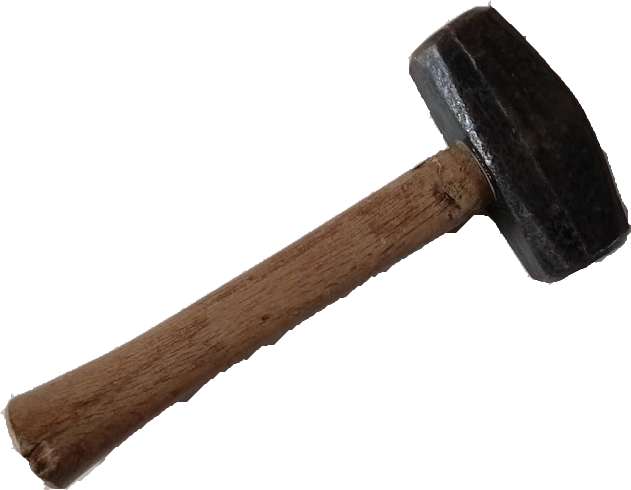
\includegraphics[height=2 \fontcharht\font`\B]{Images/hammer2crop3.png}%
	\, \textbf{\textit{HOW-TO}:}
	\endgroup
}

% This is needed for the lstset hack to preserve indentation spaces
%\usepackage[T1]{fontenc}%required

\graphicspath{{Images/}{./}} % Paths in which to look for images

\makeindex[columns=3, title=Alphabetical Index, intoc] % Make LaTeX produce the files required to compile the index

\makeglossaries % Make LaTeX produce the files required to compile the glossary

\makenomenclature % Make LaTeX produce the files required to compile the nomenclature

%----------------------------------------------------------------------------------------

\begin{document}
% Shortcuts are now centralized in their own tex file:
% Some shortcuts...
\def\BLAH{\textbf{BLAH}\xspace} % A shortcut standardizing formatting for the placeholder, BLAH
\def\non{\nonumber}
\def\python{\texttt{Python}\xspace}
\def\scipy{\htmladdnormallink{SciPy\xspace}{https://www.scipy.org/scipylib/index.html}}
\def\DS3231{\texttt{DS3231}\xspace}
\def\esp8266{\texttt{ESP8266}\xspace}
\def\MCP9808{\texttt{MCP9808}\xspace}
\def\ntp{\texttt{NTP}\xspace}
\def\rtc{\texttt{RTC}\xspace}
\def\rtcs{\texttt{RTC}s\xspace}
\def\i2c{\texttt{I2C}\xspace}
\def\gpio{\texttt{GPIO}\xspace}
\def\gpios{\texttt{GPIO}s\xspace}
\def\uart{\texttt{UART}\xspace}
\def\spi{\texttt{SPI}\xspace}
\def\adc{\texttt{ADC}\xspace}
\def\adcs{\texttt{ADC}s\xspace}
\def\matplotlib{\htmladdnormallink{matplotlib\xspace}{https://matplotlib.org}}
%\def\MScolor{ForestGreen}
\def\SNcolor{ForestGreen!25!White}
\def\MScolor{BurntOrange!25!White}
\def\Micropython{\htmladdnormallink{MicroPython\xspace}{https://http://micropython.org/}\xspace}
\def\mpfshell{\texttt{mpfshell}\xspace}  % A shortcut standardizing formatting for mpfshell
\def\thonny{\texttt{thonny}\xspace}  % A shortcut standardizing formatting for thonny
\def\webrepl{\texttt{webrepl}\xspace}  % A shortcut standardizing formatting for webrepl
\def\MFW{5cm}  % A shortcut standardizing Margin Figure Width
\def\MFWn{4cm}  % A shortcut standardizing "narrow" Margin Figure Width



%----------------------------------------------------------------------------------------
%	BOOK INFORMATION
%----------------------------------------------------------------------------------------

\titlehead{Introduction to Environmental Sensors}
% \subject{Subject}

%\title[Template for the {\normalfont\texttt{kaobook}} Class]{Template for the {\normalfont\texttt{kaobook}} Class}
\title[Foundations of Environmental Sensing]{Foundations of Environmental Sensing}
\subtitle{A practical introduction to making and using environmental sensors}

\author[DG]{Daniel Gr\"unbaum}

%\date{\today}

\publishers{Daniel Gr\"unbaum and \htmladdnormallink{www.publicsensors.org}{www.publicsensors.org}}

%----------------------------------------------------------------------------------------

\frontmatter % Denotes the start of the pre-document content
%----------------------------------------------------------------------------------------
%	OPENING PAGE
%----------------------------------------------------------------------------------------

% \makeatletter
% \extratitle{
% 	% In the title page, the title is vspaced by 9.5\baselineskip
% 	\vspace*{9\baselineskip}
% 	\vspace*{\parskip}
% 	\begin{center}
% 		% In the title page, \huge is set after the komafont for title
% 		\usekomafont{title}\huge\@title
% 	\end{center}
% }
% \makeatother

%----------------------------------------------------------------------------------------
%	COPYRIGHT PAGE
%----------------------------------------------------------------------------------------

\makeatletter
\uppertitleback{\@titlehead} % Header

\lowertitleback{
	%This book is released under a to-be-determined Creative Commons license. In the meantime \dots \\
	\textbf{Copyright: Daniel Gr\"unbaum, 2021.}
	\doclicenseThis

	\medskip

	\textbf{Colophon} \\
	This document was typeset with the help of \href{https://sourceforge.net/projects/koma-script/}{\KOMAScript} and \href{ttps://www.latex-project.org/}{\LaTeX} using the \href{https://github.com/fmarotta/kaobook/}{kaobook} class.

	\medskip

	\textbf{Publisher} \\

	First printed in November 2020 by \@publishers
}
\makeatother

%----------------------------------------------------------------------------------------
%	DEDICATION
%----------------------------------------------------------------------------------------


%\dedication{
%	The harmony of the world is made manifest in Form and Number, and the heart and soul and all the poetry of Natural Philosophy are embodied in the concept of mathematical beauty.\\
%	\flushright -- D'Arcy Wentworth Thompson
%}

%----------------------------------------------------------------------------------------
%	OUTPUT TITLE PAGE AND PREVIOUS
%----------------------------------------------------------------------------------------

% Note that \maketitle outputs the pages before here

% If twoside=false, \uppertitleback and \lowertitleback are not printed
% To overcome this issue, we set twoside=semi just before printing the title pages, and set it back to false just after the title pages
\KOMAoptions{twoside=semi}
\maketitle
\KOMAoptions{twoside=false}

%----------------------------------------------------------------------------------------
%	PREFACE
%----------------------------------------------------------------------------------------
%\setchapterstyle{kao}
%\setchapterpreamble[u]{\margintoc}
\chapter*{Preface}
\addcontentsline{toc}{chapter}{Preface} % Add the preface to the table of contents as a chapter
\labch{preface}

%\blindtext
% Adopted for first draft from Foundations of Ocean Sensing proposal, with minimal edits.
Biological, physical, chemical and geological processes in the oceans, rivers, lakes, soils and the atmosphere determine environmental conditions across our planet. 
These processes shape the past, present and future states of natural ecosystems, and the human societies that exist within them. 
Environmental sensing instrumentation is the primary means we have to measure current conditions, to infer past conditions, and to understand the mechanisms driving environmental change to make predictions about future conditions. 

Historically, at least in modern times, most environmental data have been collected by professional scientists using instruments that were specialized and costly --- and, therefore, sparse in number and accessible to very few people.
The data from these instruments are invaluable for addressing some kinds of scientific questions. 
But they are too limited to address many others, including some short-term, spatially-localized environmental variations that can have dramatic impacts on human communities and natural habitats.

Technological innovations in sensors, microcontrollers and microcomputers, power systems and data telemetry have dramatically opened access to devices that quantify and upload or store environmental data, and sharply reduced their cost.
Given current trends in governmental research funding and priorities, networks of low cost instruments deployed by students, stakeholders and other members of the public are the most promising way to quantify the present states of natural systems and the ways in which they are changing. 

Inspiration can be taken from \htmladdnormallink{WunderMap}{https://www.wunderground.com/wundermap}, an online display of real-time meteorological conditions synthesized from many thousands of personal weather stations voluntarily deployed by interested members of the public. 
By way of contrast, it's useful to compare the number of stations and the frequency of data uploads in Wundermap's crowd-sourced sensor network to the professional assets and data available from the Northwest Association of Networked Ocean Observing Systems (\htmladdnormallink{NANOOS}{http://nvs.nanoos.org/Explorer}). 
For example, where I live in the vicinity of Puget Sound, NANOOS currently displays a handful of assets, while Wundermap displays hundreds, perhaps thousands, of personal weather stations. 
So many, in fact, that you have to zoom in closely to see them all --- there are too many to display at larger scales!

Data from these sources are not equivalent.
NANOOS data are from professionally calibrated, deployed and maintained instruments, and are professionally curated, archived and stored to according exacting protocols. 
These data are intended, for example, to document decades-long processes of change in the oceans and atmosphere. 
These measurements are very sensitive to small errors in sensor calibration, and to degradation or drift in sensor readings that make comparisons across years and decades difficult.
Data from personal weather stations do not in general meet similar standards. 

On the other hand, data from modern personal weather stations typically attain impressive accuracy and precision.
These stations provide levels of redundancy, spatial and temporal resolution, and (perhaps) motivation for local communities to follow and understand environmental changes, that are orders of magnitude beyond professional scientific sensing networks. 
This comparison suggests that if members of the public had the option to acquire low cost but effective instruments to monitor habitats like shorelines, rivers, lakes, forests, etc., many of them would. 
Furthermore, the data from those instruments would be genuinely useful.

The purpose of this book is to empower readers to build and deploy inexpensive, effective environmental sensing instruments; to preserve, curate and disseminate the resulting data; and, to use those data to make scientifically informed and accurate inferences about environmental conditions and mechanisms of change. 
%\color{blue}
This book takes an experiential learning approach to convey foundational knowledge of the methods used to observe environmental characteristics -- what sensors measure, why they work, what are the requirements to use them properly, and what insights can be gained from the resulting data.
%\color{black}
Readers will also gain skills in hands-on fabrication methods, debugging and problem-solving, statistics, 

All methods of collecting environmental measurements in the environment have strengths and limitations, that impact how we design experimental observations and interpret the resulting data. 
In many cases, we cannot directly measure the environmental characteristics in which we are most interested. 
In these cases, we must use data that inform us about those characteristics indirectly, interpreting our data using models or statistical analyses. 
To effectively present the foundations of environmental sensing, this book has dual emphases on conceptual understanding and 
hands-on skills.

\subsubsection{How to use this book}
This book is a distillation and augmentation of activities and curricular materials developed for a junior-level undergraduate course in geosciences technology.
That course was designed to build on concepts and analytical skills developed in previous courses, and to prepare students to pursue upper level classes in geosciences and related fields.
Learning goals included enhanced understanding of the strengths and weaknesses of existing and future observation techniques, and practical experience and skills in building, calibrating and designing protocols using sensors for scientific purposes. 
The original activities and materials have been rewritten to be more self-contained, with more explanation and additional references to minimize reliance on assumed knowledge.

We have taught sensor-building to middle school students, to graduate students, and at all levels in between. 
We've found that, more than a specific age group, success with the activities in this book depends on a balance of engagement by students and a learning environment that supports exploration, collaboration, persistence, and occasional technical assistance.
Our goal in writing this book is to provide a roadmap and technical advice to teachers and mentors of classes and clubs for students of all ages.
With patience, and information readily available on the Internet, a highly motivated student (or, better, a collaborative group of highly motivated students) can build and use environmental sensors with little or no support from teachers or mentors.
Students working without support from teachers or mentors, however, might consider first working through tutorials in \htmladdnormallink{publicsensors.org}{https://publicsensors.org/} (or the Spanish-language equivalent, \htmladdnormallink{sensorespublicos.org}{https://sensorespublicos.org/}) before moving on to the more advanced activities and concepts in this book.

Development and use of instruments in scientific settings almost invariably requires a combination of both individual effort and collaborative work. 
The activities this book, in our experience, are far more successful when approached as an opportunity to enhance students' skills and experience in appropriately and effectively combining individual contributions with teamwork to obtain the most productive scientific outcomes. 
To be even more explicit: 
A ``MakerSpace'' atmosphere of collaborative, fun, low-stakes problem-solving transforms the inevitable troubling-shooting frustrations into creative, thought-provoking, edifying and empowering experiences.

The book is divided into three Parts:
\begin{itemize}
	\item \textsc{\textbf{Introduction}}, which introduces readers to basic skills for building circuits and communicating with microcontrollers;
	\item \textsc{\textbf{Working with environmental sensors}}, which explores the function and usage of analog and digital sensor technologies, and telemetry of resulting data; and
	\item \textsc{\textbf{Practical skills in environmental sensing}}, which covers methods of producing sensor packages that are compact and robust enough to function as practical field instruments.
\end{itemize}
Each Part comprises several chapters, which present brief background on a particular subject area, followed by guidance through a sequence of activities described in separate sections and subsections. 
Many of the activities, especially those appearing early in chapters, are cumulative --- these are helpful or essential for activities later in the book.
There is nonetheless considerable latitude for skipping activities or making them optional, especially those appearing later in chapters.
The \textbf{Skills and tools} section of the Appendix may be useful in selecting a coherent and practical subset of chapters and activities for a specific teaching situation.

Each activity is distinguished by a \howto icon, and concluded by a \textbf{Milestone} highlighted in a yellow textbox. 
\textbf{Milestone}s are specific thresholds or results, which students and their mentors can use to assess whether the key skills and experiences motivating the activity have been realized. 
To provide an overview, all the \textbf{Milestone}s are compiled in the Appendix.

Each chapter includes a list of required parts; these are also compiled (with URLs) in the Appendix.
Python scripts for running microcontrollers and for data analysis are presented both as formatted code and, more suitable for copying and pasting, as links in margin notes to online plaintext copies.
Graphics in margin notes are clickable, linked to full-sized high resolution online versions.
Additional suggestions and advice for students are highlighted in blue textboxes.
Brief explanations giving context for how and why sensors, circuits and codes work the ways they do are presented in green margin notes.

\subsubsection{How to contribute}
If you're interested in contributing corrections, new activities, or reports of using this book in formal or informal teaching settings, we'd like to hear from you! 
Please register at the forum on \htmladdnormallink{publicsensors.org}{https://publicsensors.org/} or \htmladdnormallink{sensorespublicos.org}{https://sensorespublicos.org/} and share your thoughts with us.

%
%Students who finish the course will be able to:
%\begin{enumerate}
%	\item Visualize, analyze and present data from oceanographic sensors
%	\item Design and construct simple sensors using microcontrollers (e.g. arduinos) and off-the-shelf electronic components  
%	\item Implement appropriate calibration and data archiving schemes for oceanographic sensors 
%	\item Critically assess oceanographic sensor performance, including stability, accuracy \& precision
%	\item Understand how key sensors function, and how sensor data directly or indirectly reflect key oceanographic mechanisms
%	\item Collaborate effectively in small groups or teams to design, construct and apply oceanographic sensors
%	\item Document and present methods, data and analysis effectively according to accepted scientific practice and standards
%\end{enumerate}
%



 % Preface now comes after table of contents

%----------------------------------------------------------------------------------------
%	TABLE OF CONTENTS & LIST OF FIGURES/TABLES
%----------------------------------------------------------------------------------------

\begingroup % Local scope for the following commands

% Define the style for the TOC, LOF, and LOT
%\setstretch{1} % Uncomment to modify line spacing in the ToC
%\hypersetup{linkcolor=blue} % Uncomment to set the colour of links in the ToC
\setlength{\textheight}{23cm} % Manually adjust the height of the ToC pages

% Turn on compatibility mode for the etoc package
\etocstandarddisplaystyle % "toc display" as if etoc was not loaded
\etocstandardlines % "toc lines as if etoc was not loaded

\tableofcontents % Output the table of contents

\listoffigures % Output the list of figures

%\let\cleardoublepage\bigskip
%\let\clearpage\bigskip

\listoftables % Output the list of tables

\lstlistoflistings % Output the list of listings

% Comment both of the following lines to have the LOF and the LOT on different pages
%\let\cleardoublepage\bigskip
%\let\clearpage\bigskip


\endgroup

%----------------------------------------------------------------------------------------
%	MAIN BODY
%----------------------------------------------------------------------------------------

\mainmatter % Denotes the start of the main document content, resets page numbering and uses arabic numbers
\setchapterstyle{kao} % Choose the default chapter heading style

\lstset{numbers=none}  % Formatting in listings: set to have no line numbers, so copy/paste works for python code
%\lstset{columns=flexible}
\lstset{keepspaces=true}
%\lstset{showspaces=true}
%\lstset{columns=fullflexible}
%\lstset{
%	upquote=true,
%	columns=fullflexible,
%	literate={*}{{\char42}}1
%	{-}{{\char45}}1
%}

\setchapterstyle{kao}
%\setchapterpreamble[u]{\margintoc}
\chapter*{Preface}
\addcontentsline{toc}{chapter}{Preface} % Add the preface to the table of contents as a chapter
\labch{preface}

%\blindtext
% Adopted for first draft from Foundations of Ocean Sensing proposal, with minimal edits.
Biological, physical, chemical and geological processes in the oceans, rivers, lakes, soils and the atmosphere determine environmental conditions across our planet. 
These processes shape the past, present and future states of natural ecosystems, and the human societies that exist within them. 
Environmental sensing instrumentation is the primary means we have to measure current conditions, to infer past conditions, and to understand the mechanisms driving environmental change to make predictions about future conditions. 

Historically, at least in modern times, most environmental data have been collected by professional scientists using instruments that were specialized and costly --- and, therefore, sparse in number and accessible to very few people.
The data from these instruments are invaluable for addressing some kinds of scientific questions. 
But they are too limited to address many others, including some short-term, spatially-localized environmental variations that can have dramatic impacts on human communities and natural habitats.

Technological innovations in sensors, microcontrollers and microcomputers, power systems and data telemetry have dramatically opened access to devices that quantify and upload or store environmental data, and sharply reduced their cost.
Given current trends in governmental research funding and priorities, networks of low cost instruments deployed by students, stakeholders and other members of the public are the most promising way to quantify the present states of natural systems and the ways in which they are changing. 

Inspiration can be taken from \htmladdnormallink{WunderMap}{https://www.wunderground.com/wundermap}, an online display of real-time meteorological conditions synthesized from many thousands of personal weather stations voluntarily deployed by interested members of the public. 
By way of contrast, it's useful to compare the number of stations and the frequency of data uploads in Wundermap's crowd-sourced sensor network to the professional assets and data available from the Northwest Association of Networked Ocean Observing Systems (\htmladdnormallink{NANOOS}{http://nvs.nanoos.org/Explorer}). 
For example, where I live in the vicinity of Puget Sound, NANOOS currently displays a handful of assets, while Wundermap displays hundreds, perhaps thousands, of personal weather stations. 
So many, in fact, that you have to zoom in closely to see them all --- there are too many to display at larger scales!

Data from these sources are not equivalent.
NANOOS data are from professionally calibrated, deployed and maintained instruments, and are professionally curated, archived and stored to according exacting protocols. 
These data are intended, for example, to document decades-long processes of change in the oceans and atmosphere. 
These measurements are very sensitive to small errors in sensor calibration, and to degradation or drift in sensor readings that make comparisons across years and decades difficult.
Data from personal weather stations do not in general meet similar standards. 

On the other hand, data from modern personal weather stations typically attain impressive accuracy and precision.
These stations provide levels of redundancy, spatial and temporal resolution, and (perhaps) motivation for local communities to follow and understand environmental changes, that are orders of magnitude beyond professional scientific sensing networks. 
This comparison suggests that if members of the public had the option to acquire low cost but effective instruments to monitor habitats like shorelines, rivers, lakes, forests, etc., many of them would. 
Furthermore, the data from those instruments would be genuinely useful.

The purpose of this book is to empower readers to build and deploy inexpensive, effective environmental sensing instruments; to preserve, curate and disseminate the resulting data; and, to use those data to make scientifically informed and accurate inferences about environmental conditions and mechanisms of change. 
%\color{blue}
This book takes an experiential learning approach to convey foundational knowledge of the methods used to observe environmental characteristics -- what sensors measure, why they work, what are the requirements to use them properly, and what insights can be gained from the resulting data.
%\color{black}
Readers will also gain skills in hands-on fabrication methods, debugging and problem-solving, statistics, 

All methods of collecting environmental measurements in the environment have strengths and limitations, that impact how we design experimental observations and interpret the resulting data. 
In many cases, we cannot directly measure the environmental characteristics in which we are most interested. 
In these cases, we must use data that inform us about those characteristics indirectly, interpreting our data using models or statistical analyses. 
To effectively present the foundations of environmental sensing, this book has dual emphases on conceptual understanding and 
hands-on skills.

\subsubsection{How to use this book}
This book is a distillation and augmentation of activities and curricular materials developed for a junior-level undergraduate course in geosciences technology.
That course was designed to build on concepts and analytical skills developed in previous courses, and to prepare students to pursue upper level classes in geosciences and related fields.
Learning goals included enhanced understanding of the strengths and weaknesses of existing and future observation techniques, and practical experience and skills in building, calibrating and designing protocols using sensors for scientific purposes. 
The original activities and materials have been rewritten to be more self-contained, with more explanation and additional references to minimize reliance on assumed knowledge.

We have taught sensor-building to middle school students, to graduate students, and at all levels in between. 
We've found that, more than a specific age group, success with the activities in this book depends on a balance of engagement by students and a learning environment that supports exploration, collaboration, persistence, and occasional technical assistance.
Our goal in writing this book is to provide a roadmap and technical advice to teachers and mentors of classes and clubs for students of all ages.
With patience, and information readily available on the Internet, a highly motivated student (or, better, a collaborative group of highly motivated students) can build and use environmental sensors with little or no support from teachers or mentors.
Students working without support from teachers or mentors, however, might consider first working through tutorials in \htmladdnormallink{publicsensors.org}{https://publicsensors.org/} (or the Spanish-language equivalent, \htmladdnormallink{sensorespublicos.org}{https://sensorespublicos.org/}) before moving on to the more advanced activities and concepts in this book.

Development and use of instruments in scientific settings almost invariably requires a combination of both individual effort and collaborative work. 
The activities this book, in our experience, are far more successful when approached as an opportunity to enhance students' skills and experience in appropriately and effectively combining individual contributions with teamwork to obtain the most productive scientific outcomes. 
To be even more explicit: 
A ``MakerSpace'' atmosphere of collaborative, fun, low-stakes problem-solving transforms the inevitable troubling-shooting frustrations into creative, thought-provoking, edifying and empowering experiences.

The book is divided into three Parts:
\begin{itemize}
	\item \textsc{\textbf{Introduction}}, which introduces readers to basic skills for building circuits and communicating with microcontrollers;
	\item \textsc{\textbf{Working with environmental sensors}}, which explores the function and usage of analog and digital sensor technologies, and telemetry of resulting data; and
	\item \textsc{\textbf{Practical skills in environmental sensing}}, which covers methods of producing sensor packages that are compact and robust enough to function as practical field instruments.
\end{itemize}
Each Part comprises several chapters, which present brief background on a particular subject area, followed by guidance through a sequence of activities described in separate sections and subsections. 
Many of the activities, especially those appearing early in chapters, are cumulative --- these are helpful or essential for activities later in the book.
There is nonetheless considerable latitude for skipping activities or making them optional, especially those appearing later in chapters.
The \textbf{Skills and tools} section of the Appendix may be useful in selecting a coherent and practical subset of chapters and activities for a specific teaching situation.

Each activity is distinguished by a \howto icon, and concluded by a \textbf{Milestone} highlighted in a yellow textbox. 
\textbf{Milestone}s are specific thresholds or results, which students and their mentors can use to assess whether the key skills and experiences motivating the activity have been realized. 
To provide an overview, all the \textbf{Milestone}s are compiled in the Appendix.

Each chapter includes a list of required parts; these are also compiled (with URLs) in the Appendix.
Python scripts for running microcontrollers and for data analysis are presented both as formatted code and, more suitable for copying and pasting, as links in margin notes to online plaintext copies.
Graphics in margin notes are clickable, linked to full-sized high resolution online versions.
Additional suggestions and advice for students are highlighted in blue textboxes.
Brief explanations giving context for how and why sensors, circuits and codes work the ways they do are presented in green margin notes.

\subsubsection{How to contribute}
If you're interested in contributing corrections, new activities, or reports of using this book in formal or informal teaching settings, we'd like to hear from you! 
Please register at the forum on \htmladdnormallink{publicsensors.org}{https://publicsensors.org/} or \htmladdnormallink{sensorespublicos.org}{https://sensorespublicos.org/} and share your thoughts with us.

%
%Students who finish the course will be able to:
%\begin{enumerate}
%	\item Visualize, analyze and present data from oceanographic sensors
%	\item Design and construct simple sensors using microcontrollers (e.g. arduinos) and off-the-shelf electronic components  
%	\item Implement appropriate calibration and data archiving schemes for oceanographic sensors 
%	\item Critically assess oceanographic sensor performance, including stability, accuracy \& precision
%	\item Understand how key sensors function, and how sensor data directly or indirectly reflect key oceanographic mechanisms
%	\item Collaborate effectively in small groups or teams to design, construct and apply oceanographic sensors
%	\item Document and present methods, data and analysis effectively according to accepted scientific practice and standards
%\end{enumerate}
%





\pagelayout{wide} % No margins
\addpart{Introduction}
\pagelayout{margin} % Restore margins

\setchapterstyle{kao}
\setchapterpreamble[u]{\margintoc}
\chapter{Communicating with your microcontroller}
\labch{connect}

The purpose of this book is to provide you with the necessary skills and experience to design, build and use instruments to measure environmental conditions.
The ``brain'' of these instruments is a \emph{microcontroller}.
A microcontroller is a device with a processing unit that can run codes and other instructions, and external connections (called \emph{pins}) to transmit electrical inputs and outputs.
The microcontroller is what enables your instrument to receive information from sensors, monitor and regulate its power supply, and communicate for receiving instructions and telemetering data.
Learning to communicate with and control a microcontroller is the first step in building and using environmental sensing instruments.

\subsubsection{Types of microcontrollers and single board Computers}

Microcontrollers vary by overall size, power requirements, capabilities to input and output different kinds of electrical signals, onboard communication hardware like WiFi or USB, and the types of code or instructions they accept.
They are distinct from \emph{single board computers} such as Raspberry Pis in that they generally do not incude a robust operating system or the ability to easiy send video directly to a monitor.
While they are relatively constrained in terms of memory and processor power, microntrollers have the ability to boot and/or wake quickly, reliably perform a pre-defined action such as reading a sensor and/or enabling another device, and then entering a low-power sleep mode until the next action is required.

Microcontroller chips are usually grouped with other components such as power management circuitry, external memory, USB connectors, power and/or reset switches, LEDs, crystal oscillators (used to track time), sensors, and, for those with wireless capabilities, external antennas.
These are usually arranged on a small circuitboard known as a \emph{breakout board} that provides access to the input/output pins on the chip.
A given microcontroller chip may be incorporated into hundreds or thousands of different breakout boards, each of which has slighty different capabilities.
For example a microcontroller board intended to run a small speaker embedded in toy will look very different from one intended to run a robot.
The speaker-based board may just require breaking out just one or two output pins, while the robot controller would require a large number of input/output pins as well as specialized motor control circuitry.

Systems that use microcontrollers to read a signal from a sensor and then record it to a storage device are referred to as dataloggers.
Dataloggers have been around for many decades, and commerical models have been optimized for low power use and durability.
For many environmental sensing projects, particularly those using sensors with analog voltage or current outputs, a commerical datalogger is an excellent option.
However, commercial dataloggers may not be compatible with digital sensors that require two-way communication to trigger a measurement, and they often cost much more than microcontroller boards.
Furthermore, many modern microcontrollers can also be programmed to communicate wirelessly, opening many new applications for environmental monitoring.
This textbook focuses on using low-cost microcontrollers as datalogging systems for use with both digital and analog sensors.

\subsubsection{Choosing a microcontroller language}
Choosing a microcontroller board that is suitable for a given project can be daunting.
Even within a given microcontroller family, there are many choices to make with respect to both hardware and software.
Until the early 2010s, programming microcontrollers required a specialized set of hardware and software tools.
However, with the release of the Arduino development environment, it became possible to program a variety of microcontrollers using a single framework.
When developing code for an Arduino, the program must be developed using the C programming language.
The human-readable code is then compiled and flashed to the chip, where  it automatically runs when the chip is powered up.
This process results in high performance, low latency programs. Perhaps for this reason, Ardino remains one of the most popular open-source microcontroller development frameworks.
Hoowever, because there is no easy way to interrupt an Arduino program and check the state of variables, debugging can be challenging.

This textbook focuses on microprocessors that use instructions written in \htmladdnormallink{MicroPython}{https://micropython.org/}, a subset of the \htmladdnormallink{Python}{https://www.python.org} programming language.
MicroPython is a recent invention, and a great improvement for learning about, building and using environmental sensors.
Because MicroPython-based microcontrollers are automatically interactive
\sidenote[][3cm]{\begin{kaobox}[backgroundcolor=\SNcolor,frametitlebackgroundcolor=\SNcolor,frametitle=MicroPython is \texttt{REPL}-ent!]Like Python, MicroPython runs in an interactive session.
	This session goes by the  technical-sounding name \textbf{REPL}, which stands for ``Read-Evaluate-Print-Loop''.
%	, or \emph{REPL}.
	Despite this name, REPL is a very intuitive interface.
	REPL simply means that, in a MicroPython (or Python) session, you type commands, which are then executed, and the results are displayed.
\end{kaobox}}
, they are good platforms for learning to develop and debug codes to collect data from environmental sensors. MicroPython comes in two main flavors--the standard, officially supported MicroPython release, and CircuitPython, a project supported primarily by AdaFruit, a supplier of open source electronics.  CircuitPython is based on MicroPython, but many of the libraries use slightly differnt syntax. In this textbook, all programs are based on MicroPthon, but it is relatively straightforward to convert CircuitPython code to MicroPython. For advanced users, this can be helpful becuse it opens the door to using the relatively large number of sensor device drivers that are available in CircuiPython.

Python itself is a powerful and easy to learn language for scientific computing on desktops and laptops.
If you already know some Python, you can apply that knowledge to working with MicroPython-based microcontrollers.
If you're new to Python, then by learning MicroPython you will simultaneously learn how to use Python for many other tasks.
%In fact, m
Many of the exercises in this book combine acquiring data from sensors using a microcontroller, and analyzing or plotting those data on a computer, using the same Python coding language.

%\marginnote[3cm]{Note that Python is currently undergoing a transition, from an older version (Python 2.7) to newer Python 3 versions.
%These are mostly similar, but differ in some details such as the syntax of print commands. Because MicroPython is based on Python 3, and because older versions of Python will soon no longer be supported, the codes and instructions in this book will use Python 3.}
%In most cases, Python 2.7 users will need to make only minor adjustments.
\begin{kaobox}[frametitle=Once and future Python]
	Note that Python is currently undergoing a transition, from an older version (Python 2.7) to newer Python 3 versions.
	These are mostly similar, but differ in some details such as the syntax of print commands. Because MicroPython is based on Python 3, and because older versions of Python will soon no longer be supported, the codes and instructions in this book will use Python 3.
\end{kaobox}


\begin{table}[h]%[2cm]
	\caption[\refch{connect} materials]{\textbf{Materials you'll need\dots}
%	\caption[	\textbf{\refch{connect} blah Materials you'll need\dots}
		See Table \ref{tab:materials} for additional information.}%]

		\labtab{materials_connections}
\begin{center}
			\raggedright
		%\begin{tabular}{ c c c c }
		\begin{tabular}{ c r c}
			\hline
			Sections & item & link \\
			\hline
			\multirow{3}{4em}{\refsec{connections}}
			& breadboard & \ref{mat:bb} \\
			& ESP8266 ``Feather'' & \ref{mat:mc} \\
			& micro-USB cable & \ref{mat:usb_cbl} \\
			\hline
			\multirow{1}{4em}{\refsec{WiFi_connect}}
			& WiFi router & \ref{mat:router} \\
			& WiFi USB dongle & \ref{mat:dongle} \\
			\hline
		\end{tabular}

\end{center}

\end{table}



%\section{Meet your microcontroller}
%\labsec{microcontrollers}

\subsubsection{Meet your microcontroller}
%\subsubsection{How to use this book}


For examples in this book, we will use microntroller breakout boards that comply with Adafruit's Feather form factor.
Feather-based boards incorporate a microncontroller on a somewhat standardized breakout board layout, with pins that have unique functions always (or at least usually located on a particular part of the baord.  The standardized layout allows projects built around one microcontroller to be used with another microcontroller later. This provides a modest amount of "future-proofing" for the textbook. For example, in the textbook have been tested with one of the least-expensive of the Feather boards--the Feather HUZZAH ESP8266 microcontroller.
This is a small, low-cost board with built-in WiFi that uses relatively little power.
The core ESP8266 microcontroller was originally intended to be placed in ``smart'' lightbulbs.
\sidenote[][*-7]{\begin{kaobox}[backgroundcolor=\SNcolor,frametitlebackgroundcolor=\SNcolor,frametitle=Lighten up!]See \htmladdnormallink{Tinnkerman's light bulb hacks}{https://tinkerman.cat/post/yet-another-wifi-light-bulb/} for some fun examples in which the ESP8266 microcontroller is reprogrammed in place within a smart light bulb.
Very large scale production for this purpose has made this microcontroller inexpensive, which also makes it a good choice for putting in sensors in often-harsh environments.\end{kaobox}}
Many of the characteristics designed for its intended purpose also make it suitable for environmental sensing instruments. However, soon after the release of the ESP8266 microcontroller, the manufacturer, a Chinese company known as Espressif, released a newer, somewhat similar chip known as the ESP32 that has several advantages over the ESP8266. Adafruit and other manufacturers have incorporated various version of the ESP32 into the Feather-compatible breakout boards, so all the activities originally developed for the ESP8266 should work relativelys seamlessly with the ESP32. 

Note that the exercises in this book can be successfully completed using other microcontrollers, including those mounted on boards that do not comply with the Feather form factor.
We focus here on the Feather ESP8266 because it's one of the microcontrollers officially supported by \htmladdnormallink{MicroPython}{https://http://micropython.org/}, because Adafruit provides good documentation and support for it, and because it's likely to be available for some time into the future.
The other officially supported microcontroller, Adafruit's HUZZAH ESP8266 Breakout Board, is slightly smaller and cheaper, but requires a special cable for communications rather than a generic microUSB cable.
Other manufacturers also make microcontroller boards based on the ESP8266.
Many of these will work in essentially the same way for exercises in this book.
Boards using other processors also can work.
These alternative microcontrollers may require modifying details in the MicroPython codes, such which connections are used for electrical inputs and outputs.
The \htmladdnormallink{MicroPython}{https://http://micropython.org/} website is the best reference if you are considering using alternative microprocessor boards for the activities in this book.

\begin{marginfigure}[2cm]
	\begin{center}
		\htmladdnormallink{\includegraphics[width=\MFW]{Images/ESP8266feather_top.png}}{https://publicsensors.org/IntroSensors/Images/ESP8266feather_top.png}
		\caption[ESP8266 feather microcontroller]{A ESP8266 Feather microcontroller.}
		\labfig{margin_esp8266}
	\end{center}
\end{marginfigure}

A close-up view of the ESP8266 Feather (\reffig{margin_esp8266}) shows the key features we will use to create functional environmental sensors.
\marginnote[-3.5cm]{
	The documents \htmladdnormallink{adafruit-feather-huzzah-esp8266.pdf}{https://cdn-learn.adafruit.com/downloads/pdf/adafruit-feather-huzzah-esp8266.pdf} and \htmladdnormallink{adafruit-huzzah-esp8266-breakout.pdf}{https://cdn-learn.adafruit.com/downloads/pdf/adafruit-huzzah-esp8266-breakout.pdf} are the best overall resources for information about the Adafruit Huzzah Feather and Breakout versions of the ESP8266 microcontroller.
	Please download the document for your microcontroller for future reference about specifications, pin definitions, voltage tolerances, \etc
}
The core microcontroller is the rectangular component near the bottom.
The zigzag line below it is a built-in WiFi antenna.
At the top is a connector for a microUSB cable, used to communicate with the Feather.
Plugging a USB cable into this connector and into your computer automatically supplies power to the microcontroller.
It also automatically supplies a connection for communicating with the microcontroller.% -- see \refsec{usb_connect} for instructions on how to use USB to communicate with your microcontroller.

Below and to the left of the USB connector is a button, labelled ``\texttt{RST}''.
This is a reset button, used occasionally to halt a run-away code or reboot a malfunctioning microcontroller (normally we will do this via software, so we rarely need to use the \texttt{RST} button).
At the four corners are holes for mounting screws.
Along the right and left edges are soldered ``pins'', %which are spaced to fit into a breadboard, and
which have different capabilities to transmit electrical signals to and from the microcontroller.
These pins have labels alongside (sometimes a little above or below) that identify the pin, so it can be referred to in MicroPython codes.
We will explain how to use these pins in \refch{first_exercises}.

\begin{kaobox}[frametitle=A flash of insight]
	In these exercises, we assume that your microcontroller already has the basic software needed to run MicroPython. This basic software is called ``firmware'', which must be ``flashed'' onto a microcontroller. The instructions for flashing MicroPython firmware onto your microcontroller are given at the \htmladdnormallink{Getting started with MicroPython}{http://docs.micropython.org/en/latest/esp8266/tutorial/intro.html\#intro} tutorial. If your microcontroller doesn't yet have its firmware, follow the instructions in that tutorial to get ready for the activities in this book.
\end{kaobox}



%\begin{marginfigure}[0cm]
%	\includegraphics{Images/breadboard_ESP8266feather.jpg}
%	\caption[ESP8266 feather microcontroller on breadboard]{Breadboard with ESP8266 feather.}
%	\labfig{margin_breadboard_esp8266}
%\end{marginfigure}

%%
%%\begin{lstlisting}
%%	\begin{marginfigure}
%%		\includegraphics{Images/IMG_20181205_082817686.jpg}
%%		\caption[ESP8266 feather microcontroller on breadboard, too]{Breadboard with ESP8266 feather, again.}
%%		\labfig{esp8266brd}
%%	\end{marginfigure}
%%\end{lstlisting}
%

\section{Establishing communications}
\labsec{connections}

Our starting point for building and using environmental instruments is learning how to communicate with microcontrollers from your desktop or laptop computer.
The ESP8266 Feather (and many other microcontrollers) have two primary modes of communication: USB and WiFi.
Some microcontrollers have additional communication modes, such as BlueTooth, LoRa or other wireless protocols.
However, USB and WiFi are the most common, standardized and useful communication modes for microcontrollers, so in this book we focus on these two modes.

In general, either USB or WiFi mode alone can be sufficient for building and using environmental sensors.
However, it is often very helpful to have both options.
For example, WiFi connections can be very useful when working with microcontrollers in environmental sensing instruments, which are often deployed inside waterproof housings that make it impossible to connect a cable.
On the other hand, when generating and debugging codes to run these instruments, it is frequently necessary to reboot the microcontroller.
This breaks the WiFi connection, so that the REPL session (and usually the WiFi connection itself) must be re-initiated.
In this case a USB connection, which remains active through the reboot, may be more convenient.

To work efficiently and effectively with microcontrollers, we require two essential communication functions:
\begin{enumerate}
	\item We need to issue commands and see output during a REPL session; and,
	\item We need to transfer files, such as MicroPython codes and environmental data, on and off the microcontroller's flash memory.
\end{enumerate}
Both these functions can be accomplished using either USB or WiFi.

Below, we describe two alternative approaches for communicating with  ESP8266 microcontrollers running MicroPython. Both are free, and can be implemented on most desktop and laptop computers.
\begin{itemize}
	\item Google's Chrome browser, with extensions enabling communications via USB and WiFi.
	\item \mpfshell, a command line utility (that is, a small Python script that works within a simple terminal window).
\end{itemize}
Of the two, the Chrome browser approach has the advantages that it is very easy to install on most computers, and it looks and acts very much the same across Windows, Mac OS, Chromebooks and linux computers.
However, the Chrome browser interface is slower and in some ways less capable.
Also, the only browser-based method currently available to transfer files to/from the microcontroller is through WiFi (using WebREPL, described below).

\mpfshell can both support a REPL session and transfer files, over either USB or WiFi.
The \mpfshell approach requires that Python be installed on your computer, if it is not already
(Mac OS and linux machines have Python pre-installed, but many Windows users must install it, and \mpfshell is not available for Chromebooks).
While this installation may require some extra effort, working with microcontrollers through \mpfshell is so much more effective that we recommend you take this approach whenever possible.


%\marginnote[0cm]{
\begin{kaobox}[frametitle=As you get started \dots]
One of the challenges in working with microcontrollers is that the first step -- establishing communications -- is often the fussiest part of the entire process.
That is because, while the microcontrollers are relatively standardized, the computers we use to communicate with them have highly variable and frequently changing hardware and software.
These variations may results in differences in drivers, ports and communications software between.
\emph{It's important to approach this first step patiently and systematically, and to be prepared to ask for help from experienced people in person or online.}
In addition to the instructions in this chapter, tutorials for setting up and troubleshooting USB and WiFi connections can be found at the \htmladdnormallink{MicroPython}{https://micropython.org/} website and many other resources online.
\end{kaobox}
%}


\section{Connecting to your microcontroller via USB}
We will first take you through the steps necessary to connect to your microcontroller using USB. In \refsec{WiFi_connect}, we will use this USB connection to set up your microcontroller for WiFi connections.

\subsection{Installing the driver for USB connections}
If your laptop runs Windows, OS X (Mac) or Chrome OS, you may need to install a driver to enable your computer to connect with serial USB converter on your ESP8266 Feather microcontroller (this is not needed on linux machines).
The driver is available at \htmladdnormallink{this link}{https://www.silabs.com/products/mcu/Pages/USBtoUARTBridgeVCPDrivers.aspx}.
%\todo{This link is now broken.}

Computers with older operating systems may require an older version of the driver.
If you install the newest one and still cannot connect to the microcontroller, try installing the next older one.
Note that you must \emph{uninstall} the existing driver version \emph{before} installing a different version.
Instructions are included in the downloaded package files, and on the download website.

\subsection{USB connections via the Chrome browser}
If you will use the Chrome browser for your microcontroller work, you can install it from Google's \htmladdnormallink{download page}{https://www.google.com/chrome/}.
For USB connections, you need to install an extension called \textbf{BeagleTerm}.
From a Chrome browser window, navigate to  \htmladdnormallink{this link}{https://chrome.google.com/webstore/detail/beagle-term/gkdofhllgfohlddimiiildbgoggdpoea?hl=en}, and use the button at the upper right to install it.
BeagleTerm will now appear in your list of \htmladdnormallink{Apps}{chrome://apps/}.

\begin{marginfigure}[-18cm]
	\begin{center}
		\htmladdnormallink{\includegraphics[width=\MFW]{Images/BeagleTermConnect.png}}{https://publicsensors.org/IntroSensors/Images/BeagleTermConnect.png}
		\htmladdnormallink{\includegraphics[width=\MFW]{Images/BeagleTerm.png}}{https://publicsensors.org/IntroSensors/Images/BeagleTerm.png}
%		\includegraphics[width=5cm]{Images/BeagleTermConnect.png}
		\caption[Connection via BeagleTerm.]{BeagleTerm browser windows. Upper screenshot: The connection prompt with settings. Most of these default into the correct values. The Com port setting, in this case \texttt{ttyUSB0}, is the most likely one you may need to change. Lower screenshot: After connecting, press \texttt{return} on your keyboard to start a REPL session.}
		\labfig{BeagleTermConnect}
	\end{center}
\end{marginfigure}

\subsubsection{\howto{} Connect to your microcontroller via BeagleTerm}
\begin{enumerate}
	\item \textbf{Plug a USB cable into your computer and your microcontroller (before you launch BeagleTerm)}.
	\item \textbf{Launch the BeagleTerm app.}

	Usually the default parameters are correct, if the USB cable is already connected to both the computer and microcontroller when the app launches (\reffig{BeagleTermConnect}).
	\item \textbf{Click ``Connect'' and press ``Enter'' a couple times on your keyboard.}

	You should now see a ``\verb|>>>|'' Python prompt, meaning you are connected and ready to work with your microcontroller.
\end{enumerate}
If this does not work, the culprit is usually the ``Com port'' setting.
Use the menu to try the available ports until you find the right one.

%Note that there is currently no way (other than copying and pasting) to transfer files between your computer and microcontroller via a USB cable.

\subsection{USB connections via \mpfshell}
\mpfshell is a Python-based file explorer and serial communications package.
We have found \mpfshell to be the most convenient utility for communication with ESP8266-based microcontrollers, because it includes both key communications functions.
Users can rapidly switch between interactive REPL sessions and file transfers, with a few keystrokes.
\mpfshell also works over both USB and WiFi.

%\subsubsection{To install \mpfshell:}
\subsubsection{\howto Install \mpfshell}

Instructions for installing and using \mpfshell are at \htmladdnormallink{this link}{https://github.com/wendlers/mpfshell}.
\mpfshell requires that Python be installed on your computer, preferably the most recent version (currently 3.5.9).
Machines running OS X or linux have Python pre-installed.
See links at \htmladdnormallink{Python}{https://www.python.org/downloads/windows/} and \htmladdnormallink{mpfshell}{https://gist.github.com/hardye/657385210c5d613e69cb5ba95e8c57a7} for instructions on installing Python and \mpfshell on Windows machines.
\begin{kaobox}[frametitle=Using \mpfshell in \htmladdnormallink{Integrated Development Environments}{https://en.wikipedia.org/wiki/Integrated_development_environment}  (\texttt{IDE}s)]
	\mpfshell generally works when installed and used within a \python \texttt{IDE} such as \htmladdnormallink{Enthought Canopy}{https://assets.enthought.com/downloads/}.
	\python \texttt{IDE}s can have advantages in generating and debugging code.
	However, in some cases, we have found that functions such as copying and pasting text in \texttt{REPL} sessions have been more limited within an \texttt{IDE} session than when running Python within a simple terminal.
	When possible, therefore, we recommend running \mpfshell from a simple terminal, even if you like to edit code from within an \texttt{IDE}.
\end{kaobox}

With Python3 installed, the \texttt{pip3} utility makes it straightforward to install \mpfshell and a few other Python packages it requires on Mac OS and linux computers:
\begin{enumerate}
	\item \textbf{Open a terminal window.}
	\item \textbf{Install the latest version of \mpfshell and the packages it requires.}

	On Mac OS and linux machines, use a terminal window to issue the command\sidenote[][*-8]{\begin{kaobox}[backgroundcolor=\SNcolor,frametitlebackgroundcolor=\SNcolor,frametitle=Follow the script!]In this book, we will use this format to indicate commands to be entered into a terminal window, code to be entered typed into a REPL session on your microcontroller, or lines to be put into a file to be run on your microcontroller or laptop.\end{kaobox}}
\begin{lstlisting}[language=bash]
pip3 install --upgrade --user mpfshell
\end{lstlisting}
		Note that your computer needs to be connected to the Internet to access the necessary software repositories.

		\smallskip
		On Windows machines, go to \htmladdnormallink{this link}{https://github.com/wendlers/mpfshell} and download the
		 \lstinline{mpfshell-master.zip} file using the green ``\texttt{Clone or download}'' button.
		Move this folder and unzip it in a directory of your choosing.
		Open \lstinline{Command Prompt} and navigate into the \texttt{mpfshell-master} folder within that folder.
		(To navigate through directories, type \lstinline{cd directoryname} to move into a directory called ‘directoryname’ and \lstinline{cd ..} to move out of one.)

		Then, execute the following commands in order:
\begin{lstlisting}[language=bash]
pip install -r requirements.txt
python setup.py install
\end{lstlisting}
		You should now be setup to work with \mpfshell.

		See links at \htmladdnormallink{Python}{https://www.python.org/downloads/windows/} and \htmladdnormallink{mpfshell}{https://gist.github.com/hardye/657385210c5d613e69cb5ba95e8c57a7} for further information.
\end{enumerate}

\subsubsection{\howto Connect to your microcontroller via \mpfshell:}

\begin{enumerate}
\item \textbf{Plug a USB cable into your computer and your microcontroller} (before you launch \mpfshell).
\item \textbf{Determine the correct port number.}

	On Windows computers, check the \texttt{COM} port number of your microcontroller by opening \texttt{Device Manager} and looking under the ``\texttt{Ports}'' drop down menu.

	\smallskip
	On Mac OS and linux computers, use a terminal window to issue the command
\begin{lstlisting}[language=bash]
ls -lht | head -n 30
\end{lstlisting}
%	\todo{Need instructions how to determine the com port on Windows, analogous to  on linux, Macs?}
	The output from this command is a list of the most recent ``devices'' attached to the computer.
	If you recently plugged in your microcontroller, its port name should be something like \texttt{ttyUSB0} at or near the top of this list.
	\item \textbf{Launch \mpfshell}:
	%\todo{Is being a member of the dialout group necessary to make this work without sudo?}
\begin{lstlisting}[language=bash]
mpfshell
\end{lstlisting}
	You should now see a prompt like ``\verb|mpfs [/]>|''.
	This prompt means you are in ``file transfer mode''.
	\item \textbf{Open a connection to the microcontroller, using the port name from Step 2}:
\begin{lstlisting}[language=bash]
open ttyUSB0
\end{lstlisting}
	You should get a response like ``\texttt{Connected to esp8266}''.

	\smallskip
	On some linux and Mac OS computers, a user must be a member of the \texttt{dialout} group to access devices like microcontrollers via USB.
	If you have difficulty connecting, use the command
\begin{lstlisting}[language=bash]
sudo adduser username dialout
\end{lstlisting}
	with your username substitued for \texttt{username}, to add yourself to this group.
	The \texttt{sudo} means the command should be executed as an administrator (``superuser'') so it will request a password from a qualified user.
	You may need to log off your computer and back in for this change to take effect.

\item You can now use simple commands to: \begin{itemize}
	\item \textbf{List the files} on your microcontroller (\texttt{ls}) or in your laptop's directory (\texttt{lls});
	\item \textbf{Upload a file} \textit{from} your laptop \textit{to} your microcontroller: \texttt{put blah.py}, where \texttt{blah.py} is one of the files listed by the \texttt{lls} command; or,
	\item \textbf{Download a file} \textit{from} your microcontroller \textit{to} your laptop: \texttt{get blah2.py}, where \texttt{blah2.py} is one of the files listed by the \texttt{ls} command.
\end{itemize}
Many other commands are available in \mpfshell.
You can learn about them by executing
\begin{lstlisting}[language=bash]
help
\end{lstlisting}
 or looking on the \htmladdnormallink{mpfshell github site}{https://github.com/wendlers/mpfshell}.
\item \textbf{Switch into the REPL session with the command:}
\begin{lstlisting}[language=bash]
repl
\end{lstlisting}
You should now see a ``\verb|>>>|'' Python prompt, meaning you are connected and ready to work with your microcontroller.

\item \textbf{Switch back into file transfer mode:}
When you switch into \texttt{REPL}, \mpfshell gives you a message just above the first Python prompt similar to
\begin{lstlisting}[language=bash]
*** Exit REPL with Ctrl+] ***
\end{lstlisting}
This tells you the command to switch out of the REPL session and back into file transfer mode. In this example, it's pressing the \verb|Ctrl| and \verb|]| keys on your keyboard simultaneously, but in some installations it's a different combination of keys.

\smallskip
You can switch back and forth between REPL and file transfer mode as many times as you want, as you edit your code, upload and execute it on your microcontroller, download data, \etc

\end{enumerate}
\loadMilestone{mlst:ov} % load milestone with tags id: mlst:ov}
\loadMilestone{mlst:01} % load milestone with tags id: mlst:01



\section{Connecting to your microcontroller via WiFi}
\labsec{WiFi_connect}
Your first use of the USB REPL connection will be to set up connections by WiFi.
You will then have both options as you work through other activities in this book.

\subsection{WiFi Access Points and Stations}
First, a bit of background: Your ESP8266 has two modes for its WiFi connections:
\begin{itemize}
	\item In \emph{Access Point} mode, abbreviated \texttt{AP}, your microcontroller accepts logins directly from other machines such as your laptop or desktop.
	This mode is useful, among other reasons, because when you set its name and password they do not change until you explicitly change them.
	This means that when you change locations or work in areas lacking Internet access, you can still connect with your microcontroller.

	\item In \emph{Station} mode, abbreviated \texttt{STA}, your microcontroller logs onto another, pre-existing \texttt{AP}, such your home or classroom WiFi router.
	This mode is useful, among other reasons, because it enables your microcontroller to transmit data to and from the Internet.
	However, if you change locations, previously available \texttt{AP}s will no longer be present.

	\smallskip
	If your only connection to your microcontroller is via its STA mode connection to an unavailable AP, this can lead to a conundrum in which you cannot connect to your microcontroller to give it login information to a new AP.
	For this reason, \texttt{STA} mode is usually used in conjunction with another method of connecting, such as USB or the microcontroller's own \texttt{AP} mode.

\end{itemize}

One consideration in thinking about \texttt{AP} \textit{vs}. \texttt{STA} mode for your microcontroller work is that many computer use WiFi as their primary connection to the Internet.
If your computer (like most) has only one built-in WiFi transceiver, then using it to connect to your microcontroller in \texttt{AP} mode makes it unavailable to connect to the Internet (and vice versa).
Several strategies are available to work around this problem:
If your microcontroller and your computer both connect to the same external Access Point (e.g. your home or classroom router) then you can simultaneously connect to both your microcontroller and the Internet over WiFi (but you will need to reset the router connection if you move to another location).
You can set up your microcontroller to initiate both \texttt{AP} and \texttt{STA} modes, and connect to whichever is most convenient at a given time.
On most computers, plugging in an inexpensive WiFi USB dongle (\ref{mat:dongle}) means your computer can have two WiFi connections simultaneously, connecting to both the microcontroller's \texttt{AP} and the local router.
Finally, in some situations, plugging the computer to the Internet through an ethernet cable is possible, freeing up the WiFi transceiver to connect to the microcontroller's \texttt{AP}.

\subsubsection{\howto Configure and connect to your microcontroller as an Access Point}
Your ESP8266 is by default configured as an \emph{Access Point}.
That means that it could serve as host for WiFi connections from your laptop or desktop, without making any changes.

However, by default, MicroPython sets your SSID (the name of the \texttt{AP} station, which appears as an entry in your computer's WiFi settings) to be of the format
\begin{lstlisting}[language=bash]
MicroPython-xxx
\end{lstlisting}
\verb|xxx| is different for every individual ESP8266, but if multiple microcontrollers are present these are still very similar and easily confused SSID's.
Furthermore, when they come from the factory, the default \texttt{AP}'s all have the same password (note the capital ``N''):
\begin{lstlisting}[language=bash]
micropythoN
\end{lstlisting}
That means it's easy to accidentally (or purposely) login onto the wrong microcontroller.
Not good!

To set up clearer and more secure \texttt{AP} settings:
\begin{enumerate}
	\item \textbf{Connect to your microcontroller over your USB cable, and start a REPL session.}
	\item \textbf{Query the AP status with the commands:}
\begin{lstlisting}[language=Python]
import network
ap = network.WLAN(network.AP_IF)
ap.config("essid")
\end{lstlisting}
	The output from this command is your microcontroller's original SSID.

	\item \textbf{Reset the parameters of your microcontroller's \texttt{AP} with the commands:}
\begin{lstlisting}[language=Python]
ap.config(essid="dannyESP8266", authmode=network.AUTH_WPA_WPA2_PSK, password="HakDeg?Om9")
ap.active(True)
\end{lstlisting}
	Here, the \texttt{AP} is set to have \verb|dannyESP8266| as its SSID, to have \texttt{WPA/WPA2} encryption, and to have the password ``\verb|HakDeg?Om9|''.
	Then, the \texttt{active} parameter is set to \lstinline|True|, meaning the Access Point is turned on.

	Try it with your microcontroller, with a SSID that you can easily recognize as your own, and a hard to guess password.
	%, hopefully with a password that is harder to guess than I used in this example.
	The password must be at least 8 characters long.	\sidenote[][*-4]{\begin{kaobox}[backgroundcolor=\SNcolor,frametitlebackgroundcolor=\SNcolor,frametitle=Pass the word!]The best passwords are easy to remember and hard to guess. One way to get good passwords is with a utility called \texttt{apg}. \texttt{apg} generates random passwords that are gibberish, so they're hard to guess, but pronounceable, so they're easy to remember by sound.  It is available for both \htmladdnormallink{Windows}{https://sourceforge.net/projects/apg-for-windows/} and \htmladdnormallink{Macs and linux}{https://help.ubuntu.com/community/StrongPasswords}.\end{kaobox}}


	\item \textbf{Write the SSID and password down, and put them somewhere safe.}

	\item \textbf{Log onto your microcontroller's \texttt{AP} from your computer, using the new SSID and password.}

	After a short interval, your microcontroller's configuration should appear in your computer's WiFi settings.
	Select your microprocessor's AP, and enter the password.

	When your computer successfully connects, you are ready to interact with your microcontroller over WiFi using WebREPL or \mpfshell as described below.
\end{enumerate}

Use
\begin{lstlisting}[language=Python]
ap.active(False)
\end{lstlisting}
%when you're ready to turn the AP off.
if you decide you no longer want your microcontroller's Access Point to be available.

\subsubsection{\howto Configure and connect to your microcontroller in Station mode}
\labsec{wifi_sta}
To connect your ESP8266 to the Internet the WiFi router available in your home or classroom, you need to configure your microcontroller's STA mode with that router's login information.
Let's suppose the WiFi router available in your workspace has the SSID ``\texttt{SchoolSSID}'' and the password ``\texttt{top secret!}''.
\begin{enumerate}
	\item \textbf{Connect your computer to the ``\texttt{SchoolSSID}'' WiFi AP, using the password ``\texttt{top secret!}''.}
	\item \textbf{Connect to your microcontroller over your USB cable, and start a REPL session.}
	\item \textbf{Create and set the configuration for a \texttt{STA} networking object, with the commands:}
\begin{lstlisting}[language=Python]
import network # Not necessary if you already did it in (A)
wlan = network.WLAN(network.STA_IF)
wlan.active(True)         # activate the interface
wlan.connect("SchoolSSID", "top secret!")
\end{lstlisting}
	\item \textbf{Find the IP number assigned by the router to your microcontroller, with the command:}
\begin{lstlisting}[language=Python]
wlan.ifconfig()
\end{lstlisting}
	The result will be a group of numbers enclosed in parentheses (a Python ``tuple'') similar to
\begin{lstlisting}[language=Python]
("192.168.0.9","255.255.255.0","192.168.0.1","192.168.0.1")
\end{lstlisting}
	In this output, the first entry is your ESP8266’s IP address (this is the one you care about).
	The others are the router’s network mask, gateway and DNS server addresses.
\end{enumerate}
When your microcontroller and your computer are both successfully logged onto the same Access Point, you are ready to interact with your microcontroller over WiFi using WebREPL or \mpfshell as described below.

Use
\begin{lstlisting}[language=Python]
wlan.active(False)
\end{lstlisting}
%when you're ready to turn the AP off.
if you decide you no longer want your microcontroller to try to log onto this Access Point (e.g., if you have changed location).
\sidenote{\begin{kaobox}[backgroundcolor=\SNcolor,frametitlebackgroundcolor=\SNcolor,frametitle=Stop debugging me!] A foible of the ESP8266 is that it repeatedly puts out debugging messages if it fails to connect to an Access Point when Station mode is active.
This does not interfere with interpretation of commands you send to the microcontroller, but is visually distracting.
There are two easy ways to stop this unhelpful output:
\begin{itemize}
	\item Set the \lstinline{wlan} object to inactive, with \lstinline{wlan.active(False)}; or,
	\item Turn off all debugging messages with \lstinline{import esp} and then \lstinline{esp.osdebug(None)}.
\end{itemize}
\end{kaobox}}
%	\begin{lstlisting}[language=Python]
%	\end{lstlisting}
%}
%\end{itemize}

%\marginnote[0cm]{
\begin{kaobox}[frametitle=WiFi special powers]
	One of the best features of the ESP8266 is that it's built-in WiFi can operate in both Access Point and Station mode simultaneously.
	That is, you do not have to stop the connection in AP mode to initiate a connection in station mode, or \textit{vice versa}.

	Having these two types of connections at the same time can be very useful.
	For example, if you move your microcontroller from school to home, your classroom's Access Point is no longer available.
	To connect to your home Access Point, you can log directly onto your ESP8266 using its own AP mode SSID.
	Using that connection, you can repeat the steps above, with the name and password of your home Access Point, to reconnect to the Internet.
\end{kaobox}
%}

\loadMilestone{mlst:01a} % load milestone with tags id: mlst:01a


\subsection{WiFi connections using \texttt{WebREPL} in a browser}
\texttt{WebREPL} is a way for you to use a browser window to log onto your microcontroller, when it has an active WiFi interface (either in Access Point or Station mode).
\begin{marginfigure}[0cm]
	\begin{center}
		\htmladdnormallink{\includegraphics[width=\MFW]{Images/WebREPLupload2.png}}{https://publicsensors.org/IntroSensors/Images/WebREPLupload2.png}
		\caption[A WebREPL session with upload.]{An active WebREPL session, showing the login prompt (main terminal frame) and a file upload (right side panel.}
		\labfig{WebREPL_upload}
	\end{center}
\end{marginfigure}
\texttt{WebREPL} can do both of the essential elements of communicating with microcontrollers, via a wireless connection:
It provides access to REPL, and makes it very easy to upload and download files between your laptop and the ESP8266 (\reffig{WebREPL_upload}).

%Note: Your microcontroller has to be connected via wifi for WebREPL to work, either with your laptop logged onto an Access Point created by the microcontroller, or with both your laptop and microcontroller logged onto another Access Point.

WebREPL is a free download from this	 \htmladdnormallink{link}{https://github.com/micropython/webrepl}. \sidenote[][*6]{\begin{kaobox}[backgroundcolor=\SNcolor,frametitlebackgroundcolor=\SNcolor,frametitle=Locally sourced\dots]\texttt{WebREPL} is available to use online, without installing it.
\emph{However, you will most likely want to have it actually installed directly on your computer.}
That is because, unless you have multiple internet connections available on your computer, you can’t use the online WebREPL when you connect directly to your ESP8266 as an Access Point.
You can, however, use the online \texttt{WebREPL} if your laptop and microcontroller are both logged onto another Access Point.
We recommend installing \texttt{WebREPL} on your computer because in the upcoming activities you will likely have your microcontroller connected as a station and as an access point at various times.\end{kaobox}}

An easy way to install the WebREPL archive on your machine is downloading the \htmladdnormallink{zipped package}{https://github.com/micropython/webrepl/archive/master.zip}.
Some useful introductory information on using WebREPL is provided by Adafruit
\htmladdnormallink{here}{https://learn.adafruit.com/micropython-basics-esp8266-webrepl/access-webrepl},
\htmladdnormallink{here}{https://learn.adafruit.com/micropython-basics-esp8266-webrepl/overview} and
\htmladdnormallink{here}{https://learn.adafruit.com/micropython-basics-esp8266-webrepl/send-and-get-files}.
%\begin{verbatim}
%https://learn.adafruit.com/micropython-basics-esp8266-webrepl/access-webrepl
%https://learn.adafruit.com/micropython-basics-esp8266-webrepl/overview
%https://learn.adafruit.com/micropython-basics-esp8266-webrepl/send-and-get-files
%\end{verbatim}


\subsubsection{\howto Launch WebREPL on your computer}
\begin{enumerate}
	\item  \textbf{Open the file \texttt{webrepl.html} in the \texttt{webrepl} directory}
	This is the directory that you unzipped from the archive you downloaded from \texttt{github}.
	WebREPL should work equally well in Chrome, Firefox, Chromium, Opera and other browsers.
	You should see a window like \reffig{WebREPL_upload} appear in your browser.

	\item \textbf{If necessary, enter your microcontroller's IP number in the text box at the upper left}.

	The text box at the upper left has an address that looks like
\begin{lstlisting}[language=bash]
ws://192.168.4.1:8266
\end{lstlisting}
	This has three parts:
	\begin{itemize}
		\item The first item, \verb|ws|, stands for \texttt{websocket}, the format for connecting.

		DON'T CHANGE THIS!

		\item The last item, \verb|8266|, is the port number over which to connect.

		DON'T CHANGE THIS EITHER!

		\item The middle item, \verb|192.168.4.1|, is the IP number for your microcontroller.

		There are two cases here:
	\begin{itemize}
		\item \textbf{If you are connecting to your microcontroller using its own \texttt{AP} mode, then you don't have to change anything.} The default, \verb|192.168.4.1|, is already correct.

		\item \textbf{If you are connecting to your microcontroller using its \texttt{STA} mode with a router, you will likely need to change the IP number in this box to reflect the IP assigned by the router to your ESP8266.} This is the first entry in the result of the \texttt{wlan.ifconfig()} command above.

		If you need to change the IP number, be careful not to accidentally change either of the other two items.
		If you do happen to change them, you can easily recover the defaults by pressing the reload button on your browser window.
	\end{itemize}
	\end{itemize}


	\item \textbf{Click “Connect” and enter your password after the prompt.}

	You should see the new connection reflected in a \verb|>>>| python prompt.

\end{enumerate}

%Summary: 1) Open webrepl.html in a browser; 2) Enter IP number in text box; 3) Click Connect \& enter password

%\marginnote[0cm]{
\begin{kaobox}[frametitle=Making sure \texttt{webrepl} is active on your microcontroller \dots]
\texttt{WebREPL} has two parts:
One is the web page that you open on your laptop.
The other is a Python script called \texttt{webrepl} (note the lower case!) that runs on your microcontroller.
\texttt{webrepl} must be activated for you to connect through \texttt{WebREPL}.

There are a couple of important details in making sure that \texttt{webrepl} is activated on your microcontroller:
\begin{itemize}
\item \textbf{The first time you want to connect via \texttt{WebREPL}, you need to initialize \texttt{webrepl} (set a password, \etc) by using your USB connection to issue the command}
\begin{lstlisting}[language=Python]
import webrepl_setup
\end{lstlisting}
Three things then happen:
\begin{itemize}
	\item The microcontroller will ask whether you want to ``enable'' \texttt{webrepl} (automatically start it each time the microcontroller reboots). Enter \texttt{E} to enable.
	\item The microcontroller will prompt you for a password, which you need to enter twice.
	\item The microcontroller will ask whether to reboot, which is necessary to implement your new settings (Enter \texttt{y}, for yes).
\end{itemize}
When you have finished these three steps, \texttt{webrepl} is set to start by default with the password you set when you reboot the microcontroller.

\item \textbf{If you are connected to your microcontroller via USB, sometimes \texttt{webrepl} does not run even if you set it to. In that case, you need to use your USB connection to execute the commands}
\begin{lstlisting}[language=Python]
import webrepl
webrepl.start()
\end{lstlisting}
to manually start \texttt{webrepl}. Your microcontroller will then be available to connect via the WebREPL browser window.
\end{itemize}
\end{kaobox}
%}

%\subsubsection{\howto Up- and download files over WiFi with \texttt{WebREPL}}
\texttt{WebREPL} makes it easy to transfer files from your laptop to your microcontroller and \textit{vice versa}:

\subsubsection{\howto Upload a file to your microcontroller using \texttt{WebREPL}}
\begin{enumerate}
	\item \textbf{Click on the \texttt{Browse} button at the upper right of the \texttt{WebREPL} window, under the \texttt{Send a file} prompt} (\reffig{WebREPL_upload}).
	\item \textbf{Navigate to and select the file you want to transfer} (in this example, a file called \texttt{servo.py}).
	\item \textbf{Click the \texttt{Send to device} button.}

	The textbox at the bottom of the right side panel will now report the file sent and the number of bytes uploaded.
\end{enumerate}


\subsubsection{\howto Download a file from your microcontroller using \texttt{WebREPL}}
\begin{enumerate}
	\item \textbf{List the files on the microcontroller with the \Micropython commands:}
\begin{lstlisting}[language=Python]
import os
os.listdir()
\end{lstlisting}

	\item \textbf{\textbf{Enter the name of the file to download in the textbox under the \texttt{Get a file} prompt}} (\reffig{WebREPL_download}).


	\item \textbf{Click the \texttt{Get from device} button.}
	\item \texttt{WebREPL} will download the file, report its name and size in the text box, and prompt you to save or open the file on your laptop.
	\end{enumerate}

\begin{marginfigure}[0cm]
	\begin{center}
		\htmladdnormallink{\includegraphics[width=\MFW]{Images/WebREPLdownload.png}}{https://publicsensors.org/IntroSensors/Images/WebREPLdownload.png}
		\caption[A WebREPL session with download.]{An active WebREPL session, showing the commands to list the files on the microcontroller (main terminal frame), a file download (right side panel, and a prompt for how to save or open the file.}
		\labfig{WebREPL_download}
	\end{center}
\end{marginfigure}


%\subsubsection{WiFi connections via \texttt{Secure Shell} in Chrome}
%When your microcontroller is not connected by a USB cable to your laptop, you will connect to it over WiFi.
%If \mpfshell is installed on your  machine, it is likely the best option to connect to your microcontroller over WiFi (see the \htmladdnormallink{mpfshell github site}{https://gist.github.com/hardye/657385210c5d613e69cb5ba95e8c57a7} for instructions on how to connect to a microcontroller via WiFi).
%\texttt{WebREPL} is also a good alternative, but for \texttt{WebREPL} to work it must be enabled on your microcontroller.
%If it is not enabled, and if you prefer a browser-based communication method, you can use an alternative like \htmladdnormallink{Secure Shell}{https://chrome.google.com/webstore/detail/secure-shell/pnhechapfaindjhompbnflcldabbghjo?hl=en} instead.
%
%(including logging onto your microcontroller to enable WebREPL).
%
%in some ways nicer to use than Secure Shell
%
%For this you will need a different app than you used for serial communication – you will need a terminal interface through which you can remotely log onto your microcontroller, to issue commands and obtain sensor readings.
% is an app that provides this capability.
%
%
%
%In many cases you will be able to use WebREPL instead of Secure Shell -- it also enables you to log onto your microcontroller.
%

\subsection{WiFi connections using \mpfshell}
\mpfshell is as useful for connecting to your ESP8266 remotely over WiFi as it is for connecting directly via USB.

\subsubsection{\howto Connect with your microcontroller using \mpfshell over WiFi}
\begin{enumerate}
	\item \textbf{Make sure \texttt{webrepl} is enabled (see instructions above for \texttt{WebREPL} if you're not sure).}
	\item \textbf{In a terminal window, launch \mpfshell:}
\begin{lstlisting}[language=Python]
mpfshell
\end{lstlisting}
	\item \textbf{Open the connection over WiFi with}
\begin{lstlisting}[language=Python]
open ws:192.168.4.1
\end{lstlisting}

	In this command, the number \texttt{192.168.4.1} is the microcontroller's IP number.
	If the microcontroller's \texttt{AP} is activated and your laptop is connected to it, this IP number is correct.

	If you are connecting via a router, then you need to replace this number with the IP assigned to your microcontroller (see the \texttt{wlan.ifconfig()} command in the instructions for WebREPL).

	\item \textbf{At the prompt, enter your \texttt{webrepl} password.}

	You should then see the \verb|mpfs [/]>| prompt showing that you have successfully connected through \mpfshell.
\end{enumerate}

All the \mpfshell file transfer and REPL capabilities work the same over WiFi as when connected via USB.

\loadMilestone{mlst:01b} % load milestone with tags id: mlst:01b


\section{Computing on your microcontroller using \Micropython libraries}
\labsec{mp_libs}
The great utility of \Micropython is that it makes programming and interacting with environmental sensors quick and effective.
An additional feature is that \Micropython contains many useful libraries that you can use ``out of the box'', without any external hardware.
A good source for examples and advice on using \Micropython is the \htmladdnormallink{Micropython forum}{https://forum.micropython.org/viewforum.php?f=16&sid=3b047a13be25c6522d788bfb036217a6}.
To conclude this first chapter on communicating with your microcontroller, you will implement two examples from this forum that illustrate how to generate random numbers, and how to encrypt a string of characters.
You will then anticipate later chapters in which you will telemeter environmental data over publicly available websites, by implementing a basic form of data verification.

\subsection{Generating random numbers and strings}
\labsec{rnd}
Random numbers and strings are useful for a variety of purposes in scientific data analysis and modeling.
Later in this section, we will use randomized strings to make environmental data transmissions easier to verify.
Micropython has a built-in utility, \lstinline{getrandbits} in the \lstinline{urandom} library, to generate random bits.
These random bits can then be converted into random numbers and strings. Here's how to do it:

\subsubsection{\howto Generate random numbers and strings}
A post on the \htmladdnormallink{Micropython forum}{https://forum.micropython.org/viewtopic.php?t=6158} provides an easy-to-use function that converts random bits bits into random integers in a user-supplied range.
\begin{enumerate}
	\item \textbf{To generate random integers, download} the \lstinline{random_int.py} \textbf{python script by clicking on the link in the margin. Then, use the \lstinline{<ctrl>-e/<ctrl>-d} technique to paste the following commands into a \texttt{REPL} session:}
	\lstinputlisting[language=Python,label=random_int,caption={\htmladdnormallink{\texttt{random\textunderscore int.py}}{https://github.com/publicsensors/IntroSensors/blob/main/Codes/random_int.py}: A Micropython script demonstrating generation of random integers within a specified range.}]{Codes/random_int.py}

	This code defines a function, \lstinline{randint}, that returns a single random integer between the input parameters \texttt{min} and \texttt{max} (including \texttt{min} and \texttt{max}).

	Try generating a list of random integers with a command like
\begin{lstlisting}[language=Python]
print([randint(0,999) for i in range(45)])
\end{lstlisting}
	Were you successful in generating random integers?

	\item \textbf{Generate random strings by random selections from a list of characters.}

	First, define a string containing the list of characters from which to select.
	As an example, we'll use the 26 lower case letters in the English alphabet:
\begin{lstlisting}[language=Python]
char_list=['a','b','c','d','e','f','g','h','i','j',\
           'k','l','m','n','o','p','q','r','s','t',\
           'u','v','w','x','y','z']
\end{lstlisting}
	Now, use these commands to generate a random sequence of the characters in \lstinline{char_list} that is \lstinline{str_len} letters long:
\begin{lstlisting}[language=Python]
str_len=20
rnd_str=''.join([char_list[randint(0,len(char_list)-1)] for i in range(str_len)])
print(rnd_str)
\end{lstlisting}
	In these commands, \lstinline{randint(0,len(char_list)-1)} randomly chooses the index of a character in \lstinline{char_list}.
	After this is repeated \lstinline{str_len} times to form a list of characters, the list is joined into a single string.

	Repeat these commands several times with different character lists and \lstinline{str_len} values to demonstrate that you are successfully generating random strings.

\end{enumerate}
\loadMilestone{mlst:01c} % load milestone with tags id: mlst:01c


\subsection{Encryption of character strings}
\labsec{encrypt}
\Micropython comes equipped with a basic encryption library called \lstinline{ucryptolib}.
This library is modeled after the larger  Python library \lstinline{cryptolib}, but is more limited so that it can run on microprocessors rather than full sized computers.
The encryption methods used in this library are not safe enough to be used for truly sensitive information -- with effort, they can be decrypted by an expert hacker.
Furthermore, the ``key'' to reading the data is stored on the microcontroller, so someone with physical access to the instrument could easily decrypt messages.
However, in most of our applications it's not worth anyone's trouble to decrypt environmental sensor data -- and in any case, it's not usually a secret.
The more important issue for us is being able to know that a message appearing to contain data from our sensor is genuine.
For this purpose, it's sufficient to include an encrypted password or token that an unauthorized sender is unlikely to know.

\subsubsection{\howto Encrypt and decrypt messages on your microcontroller}
With this relatively low standard of encryption in mind, let's demonstrate a basic use of \lstinline{ucryptolib} posted on the Micropython forum by \htmladdnormallink{@jimmo}{https://forum.micropython.org/viewtopic.php?t=6726}.
\begin{enumerate}
	\item \textbf{To encrypt strings, download} the \lstinline{encrypt_demo.py} \textbf{python script, and use the \lstinline{<ctrl>-e/<ctrl>-d} technique to paste the following commands into a \texttt{REPL} session:}
\lstinputlisting[language=Python,label=encrypt_demo,caption={\htmladdnormallink{\texttt{encrypt\textunderscore demo.py}}{https://github.com/publicsensors/IntroSensors/blob/main/Codes/encrypt_demo.py}: A Micropython script demonstrating simple encryption of short strings.}]{Codes/encrypt_demo.py}

	In this example,the string \texttt{input plaintext} is first placed into the variable \lstinline{data}.
	The string is then converted to bytes, and stored as the variable \lstinline{data_bytes}.

	\smallskip
	For this encryption method, the input string must be packaged in ``blocks'' of 16 bytes.
	This means that long messages must be split into shorter messages of 16 or fewer bytes, and that shorter messages must be ``padded'' by tacking on additional bytes to meet the length requirement.
	This is done in the example above by the modification of \lstinline{data_bytes} into \lstinline{data_bytes16}.
	The modified characters from the original string are then encrypted using the \lstinline{encrypt} function from \lstinline{ucryptolib}.

	\smallskip
	These steps are then repeated for the second string, \texttt{input pl}.

	The output from these commands should be
\begin{lstlisting}[language=Python]
msg1 =  b'\xfe!F\x87?\xdb\x19\x18\xcdM\x83\x9b\xaa\x02\xa9\x04'
msg2 =  b"[\x9df\xa3\xa0\xa5'\xa5v\xc1\xfeNI\xa9\x96\x03"
\end{lstlisting}
	These messages could be conveyed in a public venue, and without knowing or guessing the key (not very hard in this example) it would be difficult --- but not impossible --- for an eavesdropper to extract the original strings.

	\item \textbf{To decrypt strings, download} the \lstinline{decrypt_demo.py} \textbf{python script, and use the \lstinline{<ctrl>-e/<ctrl>-d} technique to paste the following commands into a \texttt{REPL} session:}
\lstinputlisting[language=Python,label=decrypt_demo,caption={\htmladdnormallink{\texttt{decrypt\textunderscore demo.py}}{https://github.com/publicsensors/IntroSensors/blob/main/Codes/decrypt_demo.py}: A Micropython script demonstrating simple decryption of short strings.}]{Codes/decrypt_demo.py}

	In this command sequence, the key is used to decrypt \lstinline{msg1} and  \lstinline{msg1} into the bytes from which they were generated.
	Those bytes are then converted back to strings, and the ``padding'' characters \lstinline{\x00} are removed (``stripped'')).

	The output from the decryption commands should be
\begin{lstlisting}[language=Python]
data1= input plaintext
data2= input pl
\end{lstlisting}
	which successfully recovers the original messages.

	\item \textbf{Try it with your own key and messages, taking care to split messages longer than 16 characters into shorter ones.}

	Assuming that \lstinline{\x00} was not part of the original messages, your own key should enable you to encrypt and decrypt your messages.
	If you want to include \lstinline{\x00} in your messages, you can substitute a different character as padding that does not appear in your messages.
\end{enumerate}


\subsection{Encrypted authentication of data messages}
In most uses of environmental sensors, the acquired data is not a major security concern.
That is, if we post e.g. a temperature reading to a publicly accessible website, there is usually little harm done.
Ideally, the data are relevant and well enough presented that they are helpful to other readers.
However, there is a concern if posting data makes it too easy for a viewer to mimic true data uploads by simply copying and pasting corrupted versions of past posts.
The form of encryption from \refsec{encrypt}, even though it is not unbreakable, is in general sufficient to provide a means of verifying that data uploads are genuine.

Let's consider a data message of the form
\begin{lstlisting}[language=Python]
Instrument1,Sensor3,watertemp,NorthLakeWashingtonWA,3711,2020-3-19 1:20:17,7.6875
\end{lstlisting}
from an environmental sensor similar to one you will build in later chapters of this book.
In this message, \lstinline{Intrument1} is a label for a particular \texttt{instrument}, i.e., a microcontroller that may have attached a variety of sensors.
\lstinline{Sensor3} indicates the particular sensor from which the reported datum was measured.
\lstinline{watertemp} indicates that water temperature is the environmental characteristic being measured.
\lstinline{NorthLakeWashingtonWA} is a geographical reference readable and specific enough to potentially make the data useful to others.

The actual data, in the part of the message that reads \lstinline{3711,2020-3-19 1:20:17,7.6875}, are the sample number (here, the 3711\textit{th} sample), the date/time stamp, and the temperature reading ($7.6875^\circ$).
Local residents, fishermen, limnologists and many others might find real-time reporting of water temperature from North Lake Washington to be of interest.
This is particularly true if the data from this sensor can be easily put in context with other data such as air temperature, insolation, wind speed and direction, data from elsewhere on Lake Washington, \etc

The key issue is to insure that data from another source that accidentally or intentionally look very similar to this line of data do not mistakenly get accepted into the database for this instrument.

Suppose we take a non-repeating part of this message and encrypt it, together with a \htmladdnormallink{``salt''}{https://en.wikipedia.org/wiki/Salt_(cryptography)}.
In cryptography, a salt is a string of random characters that make encrypted information like passwords harder to guess.
In our case, the sample number is always incremented after a sample, so no two samples will have the same number.
This means that even if the salt and environmental data don't change, the encrypted block will be different for every message.

We will include both the encrypted and plaintext versions of the message in the data line.
Then, any reader who can see the message can get access to the data.
However, only those with the encryption key -- us, because we placed the key on the instrument -- can decrypt the encrypted part of the message.

When we receive a message purporting to come from our instrument, we can decrypt the encrypted part of the message.
If the encrypted sample number matches the reported sample number, the message must have come from our instrument.

An eavesdropper could then resend a data message, combining our encrypted block with bogus data.
However, if that message contains a previously used sample number, we know it is bogus because we have already received data for that sample number.
If the message contains a different sample number, the encrypted and plaintext version won't match and we again know it is bogus.


\subsubsection{\howto Verify a data message}
This is a simple implementation of this message verification strategy:
\begin{enumerate}
	\item \textbf{To augment a message using encryption for verification, download} the \lstinline{encrypt_msg.py} \textbf{python script, and use the \lstinline{<ctrl>-e/<ctrl>-d} technique to paste the following commands into a \texttt{REPL} session:}
	\lstinputlisting[language=Python,label=encrypt_msg,caption={\htmladdnormallink{\texttt{encrypt\textunderscore msg.py}}{https://github.com/publicsensors/IntroSensors/blob/main/Codes/encrypt_msg.py}: A Micropython script demonstrating a simple strategy for augmenting a data message using encryption for verification.}]{Codes/encrypt_msg.py}

	In this example, both the key and the salt are strings of random letters, generated as in \refsec{rnd}.
	The key is 16 characters long (as required by the encryption algorithm), and the salt is 10 characters long so that when the sample number is added the total number of characters will not exceed 16 (we do not expect to take more than 999,999 samples!).

	In a real application, this code would be executed by the microcontroller in an instrument in the field.
	The output, in this example, is the augmented data message
\begin{lstlisting}[language=Python]
Instrument1,Sensor3,watertemp,NorthLakeWashingtonWA,3711,2020-3-19 1:20:17,7.6875,b'$\\xd8\\xd8\\xa5\\x93D\\xd1\\xb3\\xd9=\\xa8$x\\xf6n\\xce'
\end{lstlisting}
	where the rightmost entry in quotes is the encrypted block.

	\item \textbf{To verify the message using decryption, download} the \lstinline{decrypt_msg.py} \textbf{python script, and use the \lstinline{<ctrl>-e/<ctrl>-d} technique to paste the following commands into a \texttt{REPL} session:}
\lstinputlisting[language=Python,label=decrypt_msg,caption={\htmladdnormallink{\texttt{decrypt\textunderscore msg.py}}{https://github.com/publicsensors/IntroSensors/blob/main/Codes/decrypt_msg.py}: A Micropython script demonstrating decryption of an augmented data message for verification.}]{Codes/decrypt_msg.py}

	In a real application, this code would be executed on the receiving machine.
	In this demonstration, you can run it from within the \texttt{REPL} session on your microcontroller or in a Python session on your computer.

	\smallskip
	This code begins by finding the rightmost comma, and using it to separate the original message from the encrypted block.
	It then converts that block from a string back to bytes, and uses the key to decrypt it.
	This is the key verification step, because only the sender and receiver know the key.

	\smallskip
	The code then strips away the padding, and removes the salt by extracting only the digits.
	The string of digits is converted back to an integer.
	If that integer agrees with the sample number in the data, the originator of this message must have had the encryption key, and therefore be legitimate.

	\smallskip
	Note that, like most authentication schemes, this assumes that the key has not been shared and is not easy to guess.
	Furthermore, it assumes that the sample numbers are used only once, and that subsequent data lines reusing a sample number are ignored.
	Otherwise, a reader without the key could just copy both the sample number and the encrypted block, to generate a bogus but apparently verifiable data message.

\end{enumerate}

\setchapterstyle{kao}
\setchapterpreamble[u]{\margintoc}
\chapter{Circuit-building with MicroPython on the ESP8266 microcontroller}
%\chapter{First exercises with MicroPython on the ESP8266 microcontroller}
\labch{first_exercises}
This chapter covers a few concepts and skills you will need to work productively with microcontrollers. After some background, these are presented in the form of three exercises, in which you will learn: 
\begin{enumerate}
	\item How to connect your microcontroller to a platform called a \texttt{breadboard}, and how to use the microcontroller/breadboard combination to quickly assemble and troubleshoot circuits;
	\item How to use a microcontroller's electrical connections, called \texttt{General Purpose Input/Output} (\texttt{GPIO}) pins, to turn LEDs and other small devices on and off, and to respond to inputs like pressing a button; and,
	\item How to use a switch called a \texttt{relay} to turn on and off larger devices, that require too much current or voltage for your microcontroller to control directly.
\end{enumerate}

\vspace{2cm}
\begin{table}[h]
	\caption[\refch{first_exercises} materials]{\textbf{Materials you'll need\dots} 		
		See Table \ref{tab:materials} for additional information.}
	\labtab{materials_1st_exercises}
\begin{center}
		\raggedright
	%\begin{tabular}{ c c c c }
	\begin{tabular}{ c r c}
		\hline
		Sections & item & link \\
		\hline
		\multirow{3}{4em}{\refsec{breadboards}} 
		%\multirow{2}{4em}{\vrefsec{breadboards}} 
		& breadboard & \ref{mat:bb} \\
		& ESP8266 ``Feather'' & \ref{mat:mc} \\
		& micro-USB cable & \ref{mat:usb_cbl} \\
		\hline
		\multirow{3}{4em}{\refsec{circuits}}  
		%\multirow{3}{4em}{\vrefsec{circuits}}  
		& male-male jumpers & \ref{mat:jmp_mm} \\ 
		& pliers & \ref{mat:plr} \\ 
		& resistors & \ref{mat:rsts} \\ 
		\hline
	\end{tabular}

\end{center}\end{table}
%\begin{margintable}[2.cm]
%	\caption[\refch{first_exercises} materials]{\textbf{Materials you'll need\dots} 
%		
%		See Table \ref{tab:materials} for additional information.}
%	\labtab{materials_1st_exercises}
%	\raggedright
%	%\begin{tabular}{ c c c c }
%	\begin{tabular}{ c r c}
%		\hline
%		Sections & item & link \\
%		\hline
%		\multirow{3}{4em}{\refsec{breadboards}} 
%		%\multirow{2}{4em}{\vrefsec{breadboards}} 
%		& breadboard & \ref{mat:bb} \\
%		& ESP8266 ``Feather'' & \ref{mat:mc} \\
%		& micro-USB cable & \ref{mat:usb_cbl} \\
%		\hline
%		\multirow{3}{4em}{\refsec{circuits}}  
%		%\multirow{3}{4em}{\vrefsec{circuits}}  
%		& male-male jumpers & \ref{mat:jmp_mm} \\ 
%		& pliers & \ref{mat:plr} \\ 
%		& resistors & \ref{mat:rsts} \\ 
%		\hline
%	\end{tabular}
%\end{margintable}


\section{Assembling circuits with microcontrollers and breadboards}
\labsec{breadboards}
For the purposes of this book, a \emph{circuit} is simply an assembly of wires and other electrical components intended to perform a useful task. 
Circuits need not be complicated --- a circuit consisting of only a battery, a wire, a switch and a light bulb is enough to make a flashlight, which can be very useful! 

Like this example, most circuits share a few common features, such as:
\begin{itemize}
	 \item A power source (or connections to attach one);
	 \item One or more components to regulate power, such as switches or resistors; and,
	 \item One or more components that convert electrical signals into physical effects (such as emitting light or turning a motor) or, alternatively, convert physical parameters into electrical signals (such as temperature or light sensors). 
\end{itemize}

In general, complicated circuits are built out of combinations of simpler ``sub-circuits''. Sub-circuits are parts of the overall circuit, that each have an identifiable and testable function. 
This \emph{modular} circuit design means that, if you start with simple circuits and understand them individually before they go into a complex circuit, the end result is easier to understand than if you contemplate an entire complex assembly at once. 
This sub-circuit based design is helpful for trouble-shooting as well.
%\sidenote[][*-12]{
	\begin{kaobox}[frametitle=Divide and conquer!]
		The key tactic of testing and debugging circuits is ``divide and conquer'': 
		If a complex circuit doesn't work (they usually don't, at first) try to divide it into two or more smaller, simpler sub-circuits.
		Then you can more easily assess which of these sub-circuits is causing the problem. 
		Often this has to be done multiple times, dividing a circuit into smaller and smaller parts until a problem is evident in one or more of them. 
		Having fixed the sub-circuit, work the other way by gradually reassembling larger subsets of components. 
		At the end of this process, the entire circuit will function as intended!
	\end{kaobox}
%}

For example, later in this Chapter, you will assemble a circuit enabling your microcontroller to ``snooze'' (slowly brighten and dim) an LED, in response to pressing a button. 
This circuit will comprise three  simpler sub-circuits, each responsible for a different task. 
One sub-circuit will distribute power to where it's needed in the circuit. 
Another will enable your microcontroller to detect when you press a button. 
The third will enable your microcontroller to turn power on and off to an LED. 
Because each of these sub-circuits has an identifiable, relatively simple function, each can be assembled and tested independently of the other sub-circuits. 
When all of these sub-circuits are working correctly, they will be linked together to form the complete circuit. 
This circuit will combine all the sub-circuits' functions to perform the intended task: suppling power to an LED regulated by the microcontroller in response to your pressing a button. 

Most of the exercises in this book will involve building, testing, troubleshooting and fixing one or more circuits. 
Initially this may feel unfamiliar.
After you have assembled your first few circuits, though, it will quickly come to feel much easier and more intuitive.

\subsection{Breadboard basics}
\begin{marginfigure}[-10.cm]
	\begin{center}
		\htmladdnormallink{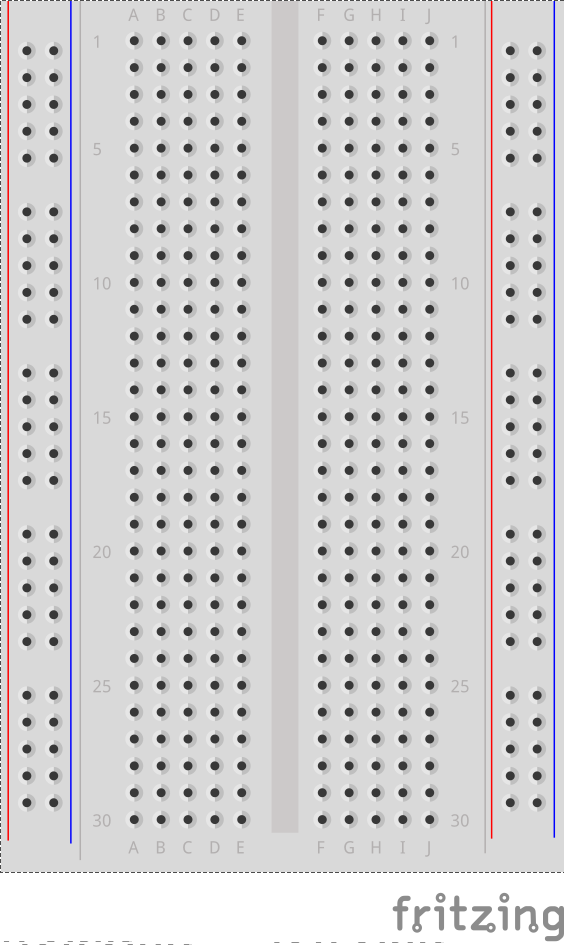
\includegraphics[width=\MFWn]{Fritzing/breadboard_bare.png}}{https://publicsensors.org/IntroSensors/Fritzing/breadboard_bare.png}
		\htmladdnormallink{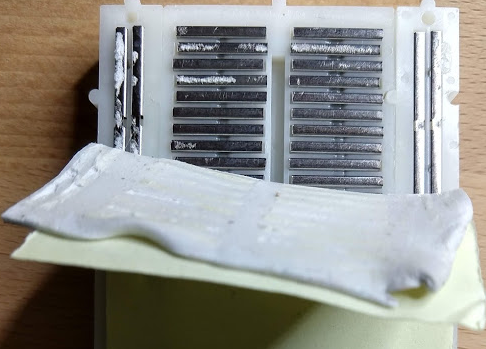
\includegraphics[width=\MFWn]{Images/breadboard_back1_crop.png}	}{https://publicsensors.org/IntroSensors/Images/breadboard_back1_crop.png}
		\caption[Breadboard front/back]{Breadboard front view, and back view with wires partly exposed.}
		\labfig{margin_breadboard}
	\end{center}
\end{marginfigure}
In the world of electronics, a \emph{breadboard} is a plastic or ceramic plate containing a large number of holes. 
Within the breadboard are hidden internal wires, connected in special patterns (\reffig{margin_breadboard}). 
When a wire is inserted into a breadboard hole, it makes an electrical connection with the hidden wires beneath, and is thereby connected to a specific set of other holes. %, \reffig{marginbb_schematic}). %\cref{margin_breadboard,marginbb_schematic}.  
The geometry of these holes and hidden wires is designed to make assembling and modifying circuits simple and fast, and to make it easy to understand connections among components. 

\emph{Prototyping} is the overall process of designing, assembling, correcting and enhancing new circuits. 
In prototyping, it is common (and usually harmless) to make small mistakes. 
Also, prototyping often involves some guesswork and iteration about \emph{layout} (e.g., which components should go next to which, to make wiring as compact and simple as possible).
The holes in breadboards are shaped so that wires (often called \emph{jumpers}\sidenote[][*-4]{\begin{kaobox}[backgroundcolor=\SNcolor,frametitlebackgroundcolor=\SNcolor,frametitle=Wire we using jumpers?]
	To make electrical connections on a breadboard, we use wires called ``jumpers''. 
	Jumpers are mostly covered with insulation, to avoid accidental connections (``short circuits''). 
	However, the last few millimeters on both ends are \emph{stripped} (the insulation is removed) so that they fit into the breadboard. 
	You can buy jumpers in several different forms, or make them yourself out of thin solid core wire. 
	In our lab, we have lots of old ethernet cable, with 8 strands of wire that is perfect for making jumpers. 
	Store-bought jumpers seem much more expensive than they ought to be, so we encourage you to make your own whenever possible.\end{kaobox}}) can be easily inserted and removed from them.
When you find a mistake or want to change the circuit design, it is straightforward to add wires, or to pull existing wires out of their present holes and move them into new holes.
Breadboards are useful, among other reasons, because they help make this process of circuit prototyping more straightforward and efficient
%\sidenote[][*-0]{
%	For sensors intended to function in the environment, sometimes it is sufficient to use a circuit built on a breadboard. 
%	Other times, however, circuits must be made as small as possible (e.g. to fit into a waterproof housing), resistant to vibrations, etc.
%	In these cases, it may helpful to use soldered connections on a \htmladdnormallink{``stripboard''}{https://en.wikipedia.org/wiki/Stripboard} or a Printed Circuit Board (PCB). 
%	This is usually done after a fully functional prototype is developed on a breadboard.
%	For instructions on how to make your own PCBs, see \refch{PCB_design}.
%}
%\begin{marginfigure}[-0.cm]
%	\begin{center}
%			\htmladdnormallink{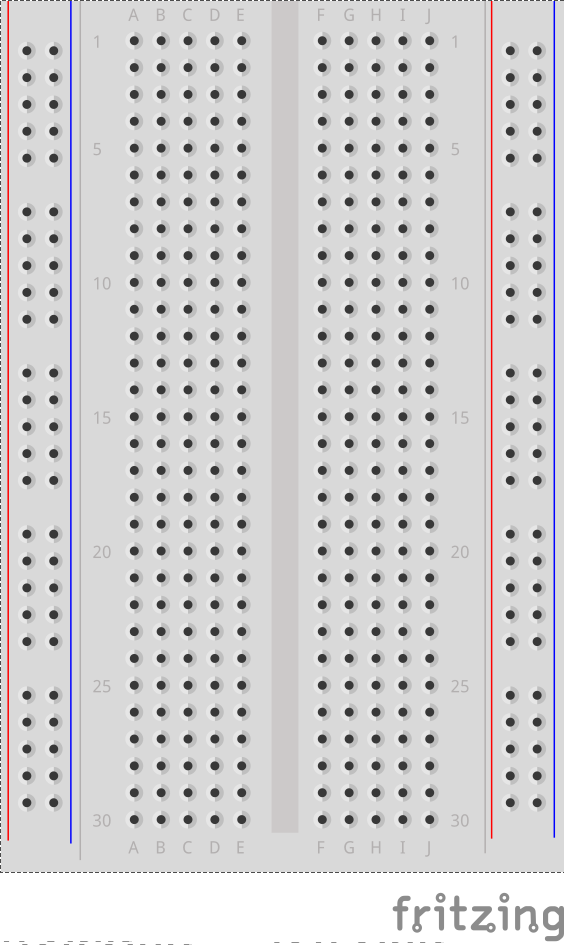
\includegraphics[width=\MFWn]{Fritzing/breadboard_bare.png}}{https://publicsensors.org/IntroSensors/Fritzing/breadboard_bare.png}
%			\htmladdnormallink{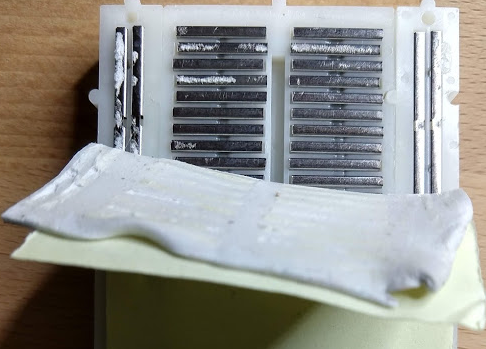
\includegraphics[width=\MFWn]{Images/breadboard_back1_crop.png}	}{https://publicsensors.org/IntroSensors/Images/breadboard_back1_crop.png}
%		\caption[Breadboard front/back]{Breadboard front view, and back view with wires (partly) exposed.}
%		\labfig{margin_breadboard}
%	\end{center}
%\end{marginfigure}

%In comparison to tweaking a circuit that is soldered together, working with breadboards is much faster and easier! 
%After a little experience, it will become almost automatic to follow connections on a breadboard to tell how a circuit is laid out and what it does. 

The holes on breadboards are laid out in \emph{rows} and \emph{columns}. 
The interior section of a typical breadboard has two rectangular blocks of holes, with five holes in each row on each side of a ``gutter''. 
In these interior sections, the five holes within one row on either side of the gutter are connected by a hidden wire. 
However, holes in one row are not connected to holes in other rows. 
Furthermore, holes on one side of the gutter are not connected to the holes on the other side (\reffig{marginbb_schematic}).

The breadboard's hidden connections mean that any set of wires inserted into holes in the same row on the same side of the gutter are connected. 
On the other hand, any wires inserted into holes in different rows, or in the same row but on opposite sides of the gutter, are \emph{insulated} from each other (not connected). 
This straightforward geometry simplifies makes it easy to understand the layout of an existing circuit, or to build a new one. 
 
Alongside the interior blocks of holes, most breadboards have paired columns of holes. 
Unlike the interior holes, these exterior sets of holes are connected in columns but not in rows. 
These exterior columns of holes, sometimes called \emph{rails}, are usually reserved for purposes such as supplying power to components distributed across the breadboard. 

\begin{marginfigure}[-4 cm]
	\begin{center}
		\htmladdnormallink{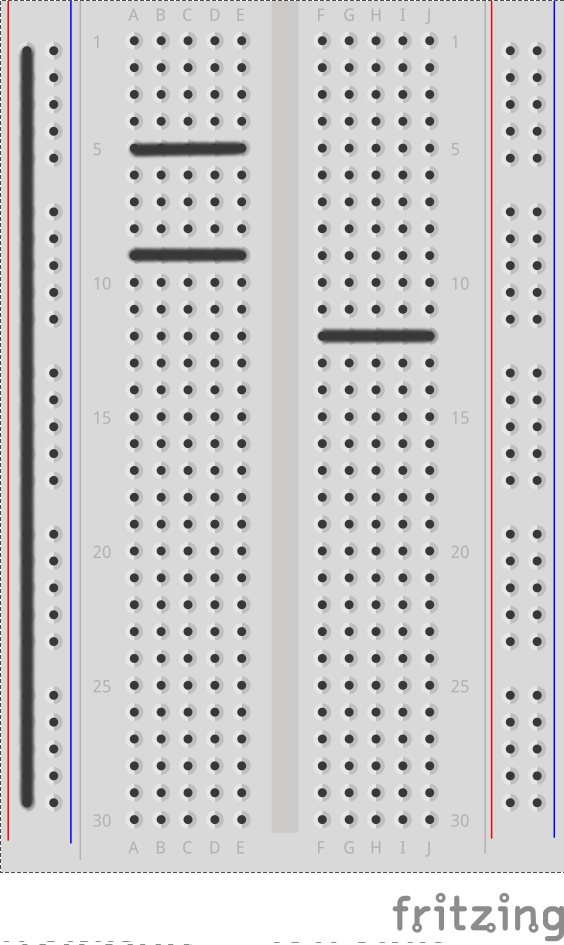
\includegraphics[width=\MFW]{Fritzing/breadboard_connections.png}}{https://publicsensors.org/IntroSensors/Fritzing/breadboard_connections.png}
		\caption[Breadboard connections schematic]{An illustration of the connections provided by hidden wires in a typical breadboard. The five holes in each interior row are connected, as indicated by the horizontal black lines. The gray vertical line is the ``gutter'' --- holes on opposite sides of the gutter are \underline{not} connected. Holes are also connected in exterior columns (called ``rails''), indicated here by the vertical black line.}
		\labfig{marginbb_schematic}
	\end{center}
\end{marginfigure}

One of the rails on each side is often marked with a ``+'' or a red line (\reffig{marginbb_schematic}). 
This column is usually attached to the positive terminal of a battery or power supply.
The corresponding rail might be marked with a ``-'' or a blue line.
This column is usually attached to the negative or \emph{ground} terminal. 
These rails make it possible to supply power and ground connections to components anywhere on the breadboard, using only very short wire connections that are visually neat and have minimal crossings. 
Circuits laid out with short, neat connections are usually easier to assemble and troubleshoot than equivalent circuits laid out with long loopy or crisscrossing wires.

Breadboards come in a wide range of different sizes and shapes, suitable for different kinds of projects. 
Smaller breadboards may have only a few rows, and may lack power and ground rails. 
Larger breadboards may be composed of several subunits, each of which has independent interior sections and rails.  
Despite differences in size, however, the same basic geometry of hidden wires connecting interior rows and (if present) exterior columns applies to all of these breadboard configurations.

%\section{Meet your microcontroller}
%\labsec{microcontrollers}
%Now it's time to start working with your microcontroller. 
%To begin with, a little background about microcontrollers: 
%A \emph{microcontroller} is a device with a processing unit that can run codes and other instructions, and with external connections (called \emph{pins}) to transmit electrical inputs and outputs. 
%There exist many types of microprocessors, which vary by overall size, power requirements, capabilities to input and output different kinds of electrical signals, onboard communication hardware like WiFi or USB connectors, and the types of code or instructions they accept. 
%
%This textbook focuses on microprocessors that use instructions written in \htmladdnormallink{MicroPython}{https://micropython.org/}, a subset of the \htmladdnormallink{Python}{https://www.python.org} programming language.
%MicroPython is a recent invention, and a great improvement for learning about, building and using environmental sensors.
%Because MicroPython-based microcontrollers are automatically interactive
%\sidenote[][*-6]{Like Python, MicroPython runs in an interactive session. 
%	This session goes by the  technical-sounding name ``Read-Evaluate-Print-Loop'', or \emph{REPL}. Despite this name, REPL is a very intuitive interface. 
%	REPL simply means that, in a MicroPython (or Python) session, you type commands, which are then executed, and the results are then displayed.
%}
%, they are good platforms to develop and debug codes to collect data from environmental sensors.  
%Python itself is a powerful and easy to learn language for scientific computing on desktops and laptops. If you already know some Python, you can apply that knowledge to working with MicroPython-based microcontrollers. If you're new to Python, then by learning MicroPython you will simultaneously learn how to use Python for many other tasks. In fact, many of the exercises in this book combine acquiring data from sensors, and analyzing or plotting those data on a computer, using the same coding language!
%  
%\subsubsection{Adafruit's Feather HUZZAH ESP8266 microcontroller}
%
%\begin{marginfigure}[-18cm]
%	\begin{center}
%			\includegraphics[height=6cm]{Images/ESP8266feather_top.png}
%		\caption[ESP8266 feather microcontroller]{A ESP8266 Feather microcontroller.}
%		\labfig{margin_esp8266}
%	\end{center}
%\end{marginfigure}
%
%For examples in this book, we will use Adafruit's Feather HUZZAH ESP8266 microcontroller. 
%It is small, has built-in wifi, uses relatively little power, and is low cost for its capabilities. 
%The core ESP8266 microcontroller was originally intended to be placed in ``smart'' lightbulbs.\sidenote[][*+8]{See e.g. \htmladdnormallink{Tinnkerman's light bulb hacks}{https://tinkerman.cat/post/yet-another-wifi-light-bulb/} for some fun examples in which the ESP8266 microcontroller is reprogrammed in place within a smart light bulb.}
%Very large scale production for this purpose has made this microcontroller inexpensive, which also makes it a good choice for putting sensors in often-harsh environments.
%
%Note that the exercises in this book can be successfully completed using other microcontrollers. 
%We focus here on the Feather ESP8266 because it is one of the microcontrollers officially supported by \htmladdnormallink{MicroPython}{https://http://micropython.org/}, and because Adafruit provides good documentation and support for it.
%Other manufacturers also make microcontroller boards based on the ESP8266. 
%Many of these will work in essentially the same way. 
%Boards using other processors also can work, but may require modifying details such as pin numbers. 
%The \htmladdnormallink{MicroPython}{https://http://micropython.org/} website is the best reference if you are considering using alternative microprocessor boards for the activities in this book.
%
%
%A close-up view of the ESP8266 Feather (\reffig{margin_esp8266}) shows the key features we will use to create functional environmental sensors.
%\marginnote[-0cm]{
%	The documents \htmladdnormallink{adafruit-huzzah-esp8266-breakout.pdf}{https://cdn-learn.adafruit.com/downloads/pdf/adafruit-huzzah-esp8266-breakout.pdf} and  \htmladdnormallink{adafruit-feather-huzzah-esp8266.pdf}{https://cdn-learn.adafruit.com/downloads/pdf/adafruit-feather-huzzah-esp8266.pdf} are the best overall resources for information about the Adafruit Huzzah Breakout and Feather versions of the ESP8266 microcontroller. 
%	Please download the document for your microcontroller for future reference about specifications, pin definitions, voltage tolerances, etc.
%}
%The core microcontroller is the rectangular component near the bottom.
%The zigzag line below it is a built-in WiFi antenna. 
%At the top is a connector for a microUSB cable, used to communicate with the Feather. 
%Plugging a USB cable into this connector and into your computer automatically supplies power to the microcontroller. 
%It also automatically supplies a connection for communicating with the microcontroller -- see \refch{connect} for instructions on how to use USB to communicate with your microcontroller.
%
%Below and to the left of the USB connector is a button, labelled ``\texttt{RST}''. 
%This is a reset button, used occasionally to halt a run-away code or reboot a hung or malfunctioning microcontroller (normally we will do this via software, so we rarely need to use the \texttt{RST} button).
%At the four corners are holes for mounting screws. 
%Along the right and left edges are soldered pins, which are spaced to fit into a breadboard, and which have different capabilities to transmit electrical signals to and from the microcontroller. 
%These pins have labels alongside (sometimes a little above or below) that identify the pin. 
%We will learn more about how to use these pins in the next section. 


%
%\begin{lstlisting}
%	\begin{marginfigure}
%		\includegraphics{Images/IMG_20181205_082817686.jpg}
%		\caption[ESP8266 feather microcontroller on breadboard, too]{Breadboard with ESP8266 feather, again.}
%		\labfig{esp8266brd}
%	\end{marginfigure}
%\end{lstlisting}

%\sidenote[][*-0]{
%\begin{kaobox}[frametitle=Beyond breaboarding \dots]
\begin{kaobox}[frametitle=Board with circuit design \dots]
	For sensors intended to function in the environment, sometimes it is sufficient to use a circuit built on a breadboard. 
	Other times, however, circuits must be made as small as possible (e.g. to fit into a waterproof housing), be resistant to vibrations, etc.
	In these cases, it may helpful to use soldered connections on a \htmladdnormallink{``stripboard''}{https://en.wikipedia.org/wiki/Stripboard} or a Printed Circuit Board (PCB). 
	This is usually done after a fully functional prototype is developed on a breadboard.
	For instructions on how to make your own PCBs, see \refch{PCB_design}.
\end{kaobox}%}

\subsection{Using General Purpose Input/Output (GPIO) pins}
Microcontrollers are useful because they are able to transmit and receive electrical signals to and from other devices.
These signals are passed through connections called \texttt{General Purpose Input/Output} pins, usually abbreviated as \texttt{GPIOs}.  

Before we say anything else about GPIOs, we'll say this: 

\color{red} \textbf{GPIOs on the ESP8266 have a voltage limit of \texttt{3.3 volts}! Be careful not to attach a GPIO to a voltage higher than \texttt{3.3 V} --- it can destroy your microcontroller!} \color{black}

Other important things to know about GPIOs on the ESP8266 are:
\begin{itemize}
	\item[$\bullet$] Pins labeled with numbers (0, 2, 4, 5, 12, 13, 14, 15 and 16) are GPIOs.
	\item[$\bullet$] GPIOs can be set by software commands to work as either \emph{input} or \emph{output} pins (but not both simultaneously).
	 \begin{itemize}
		\item[$\circ$] In output mode, a GPIO is set by the microcontroller to take on a specific voltage. 
		\item[$\circ$] Output mode is typically used when the microcontroller needs to \underline{send} a signal.
		\item[$\circ$] In input mode, a GPIO is set by the microcontroller to detect the voltage supplied to the pin by another component. 
		\item[$\circ$] Input mode is typically used when the microcontroller needs to \underline{receive} a signal.
	\end{itemize}
	\item[$\bullet$] These GPIOs are \emph{digital}. This means that these pins can only take one of two values:
	 \begin{itemize}
	 	\item[$\circ$] 1, or ``high'', corresponding to a voltage $> 1.5$ \texttt{volts}\sidenote[][*0]{\begin{kaobox}[backgroundcolor=\SNcolor,frametitlebackgroundcolor=\SNcolor,frametitle=What's your limit?]Note that the \texttt{1.5 volt} threshold applies to the ESP8266, and to many other microcontrollers. 
	 		Some have different thresholds, though, so if you're using a different microcontroller it's a good idea to check.\end{kaobox}}; or,
	 	\item[$\circ$] 0, or ``low'', corresponding to a voltage $le 1.5$ \texttt{volts}.
	\end{itemize}
	\item There is one other pin on the ESP8266, labeled \texttt{ADC} (for Analog to Digital Conversion), that can measure any voltage between 0  and 1 \texttt{volts}. \refch{circuits_intro} explains how to use the \texttt{ADC} pin to measure battery level, get readings from analog environmental sensors, \etc
%	this threshold is )\texttt{GND} or 0 volts; or, 
%	 	, above a specific threshold (for the ESP8266, this threshold is ); or,	 
\end{itemize} 
With this background, it's time to learn what GPIOs can do by building some simple circuits!

\subsubsection{GPIOs as outputs}
Your first activity with your microcontroller will be to use GPIO pins as \emph{outputs}. 
This means that you will use MicroPython commands to set the on/off state of specific pins. 
Using GPIOs in their other mode, as \emph{inputs}, will come in the next section.

The ESP8266 Feather has two built-in LEDs, that are connected inside the microcontroller board to two of the GPIO pins. 
\begin{itemize}
	\item[$\circ$] Pin 0 is connected to a red LED. 
	\item[$\circ$] Pin 2 is connected to a blue LED.
\end{itemize}
Because these LEDs are already present without need for external connections, and because they make visible the state of the pins they connect with, they make a good starting point for learning to use GPIOs.

\subsubsection{\howto Turn on/off the on-board LEDs}
To control the red LED, you will use the \lstinline{Pin} method from Micropython’s \lstinline{machine} package.
\begin{marginfigure}[-2cm]
	\htmladdnormallink{\includegraphics[width=\MFW]{Images/breadboard_ESP8266feather.jpg}}{https://publicsensors.org/IntroSensors/Images/breadboard_ESP8266feather.jpg}
	\caption[ESP8266 feather microcontroller on breadboard]{Breadboard with ESP8266 feather.}
	\labfig{margin_breadboard_esp8266}
\end{marginfigure}

%\sidenote{
%	In this section, we assume you have already established communications with your microcontroller. 
%	If you have not yet done that, please see %\refpart{conns} %
%	\refch{connect} %\refch{usb_connect} and \refch{wifi_connect} 
%	for instructions before proceeding.}
\begin{enumerate}
	\item \textbf{Mount your microcontroller on a breadboard and connect a USB cable, as shown in \reffig{margin_breadboard_esp8266}.} 
	
	\begin{itemize}
		\item[$\circ$] Note that the USB connector is facing upwards, off the board, to make it easy to reach. 
		\item[$\circ$] The first row of pins projecting below the board are inserted into the breadboard in the top row of breadboard holes. 
		
		This is to leave as many rows below the ESP8266 as possible accessible for circuit-building. 
	
		\item[$\circ$] The microcontroller fits onto the breadboard either with one open column of holes on the left and two on the right, or with two on the left and one on the right. 
		
		\smallskip
		For this set of exercises, either position is OK.
	\end{itemize} 
%is mounted on a On your ESP8266, each of the numbered pins inserting into your breadboard is a GPIO. Each of these is available for transmitting and receiving signals, although some of these pins also have other functions.

	\item \textbf{Open a \texttt{REPL} session}
	
	\item \textbf{Import the \texttt{Pin} class}:%\sidenote[][*-0]{In this book, we will use this format to indicate code to be entered typed into a REPL session on your microcontroller, or to be put into a file to be run on your microcontroller or laptop.}:
\begin{lstlisting}[language=Python]
from machine import Pin 
\end{lstlisting}	

	\item \textbf{Create a \texttt{Pin} object pointing to \texttt{GPIO 0}, setting that pin into output mode}:
\begin{lstlisting}[language=Python]
pin0 = Pin(0, Pin.OUT) 
\end{lstlisting}	
	
	\begin{itemize}
		\item[$\circ$] In this Python statement, \texttt{pin0} is the name of the object to be created. 
		This name could in general be almost anything, but it's a good idea to make names as informative as possible. 
		In this case, ``pin'' will remind us that it's a \texttt{Pin} object, and the ``0'' reminds us that it points to \texttt{GPIO 0}.
	
%	\smallskip
	
	\item[$\circ$] Inside the call to the \texttt{Pin} method, the \texttt{0} indicates the object will be attached to \texttt{GPIO 0}, and \texttt{Pin.OUT} sets that GPIO into output mode.
	\end{itemize}
 
	\item \textbf{Use the \texttt{pin0} object to query or set the state of this pin, by entering the follows commands}:
\begin{lstlisting}[language=Python]
pin0.value()  # returns the present state of GPIO 0
pin0.value(1) # sets state of GPIO 0 to 1, or ``on''
pin0.value()  # returns the present state of GPIO 0
pin0.value(0) # sets state of GPIO 0 to 0, or ``off''
pin0.value() # returns the present state of GPIO 0
\end{lstlisting}
	Note that \texttt{pin0.value(1)} causes \texttt{GPIO 0} to be set at \texttt{3.3 volts}.
	\texttt{pin0.value(0)} causes GPIO 0 to be set at \texttt{0 volts}.
	Which of these corresponds to the red LED turning on? Is that what you expected? 
	
	\item \textbf{Control pin state with } \lstinline{on} \textbf{and} \lstinline{off}.
	The pin object also allows you to use \lstinline{pin0.on()} and \lstinline{pin0.off()} to set the state of a GPIO in output mode. 
	Try this and verify that you can toggle the LED on and off.
	Keep in mind, though, that this notation can be confusing. 
	For example, in some circuits, invoking \lstinline{pin0.on()} turns an attached device  off, and \textit{vice versa}. 
	To avoid ambiguity, we usually stick with the \lstinline{pin0.value()} method when using GPIOs.
	
	\item \textbf{Repeat the steps above, but this time create an object pointing to \texttt{GPIO 2}.}
	
	\emph{Things to think about \dots}
	\begin{itemize}
		\item What is an informative name for this new object? 
		\item What is the behavior of the microcontroller when you execute these commands?
	\end{itemize}
\end{enumerate}

%%\begin{kaobox}[frametitle=Milestones Overview]
%%	\begin{itemize}
%%		\item 
%\marginnote[-5cm]{
%		\loadMilestone{mlst:ov} % load milestone with tags id: mlst:ov}%	\end{itemize}
%}%\end{kaobox}
%
%%{\color{orange} \rule{\linewidth}{0.5mm} }
%%\begin{kaobox}[frametitle=Using GPIOs as outputs]
%%	\begin{itemize}
%%		\item[$\Box$] 
%\marginnote[0cm]{
%		\loadMilestone{mlst:02a} % load milestone with tags id: mlst:02
%}%	\end{itemize}
%%\end{kaobox}
%%{\color{orange} \rule{\linewidth}{0.5mm} }


\loadMilestone{mlst:02a} % load milestone with tags id: mlst:02

%\marginnote[0cm]{
	\begin{kaobox}[frametitle=Some MicroPython shortcuts...] \label{copy_paste}
	Micropython has shortcuts that can save you lots of typing. 
	\begin{itemize}
	\item[$\bullet$] Hitting the up arrow ($\uparrow$) parses through previous commands so you can edit and re-execute them.
	\item[$\bullet$] To paste in a block of formatted python code (e.g. from a python editor on your laptop), type 
\begin{lstlisting}[language=Python]
<ctrl>-e
[pasted python code]
<ctrl>-d
\end{lstlisting}
	As an example, copy the code you used to control the red LED, and paste it into an editor on your laptop. 
	Now, use the \texttt{<ctrl>-e}/\texttt{<ctrl>-d} sequence to paste this code to the ESP8266. 
	The pasted code will be executed when you type the \texttt{<ctrl>-d}.

	\item  \texttt{<ctrl>-d} by itself (that is, not preceeded by \texttt{<ctrl>-e}) reboots the ESP8266! 
	This causes the Micropython session to “forget” all the previous commands and clear all its memory. 
	In Python, it is not possible to import a library twice. 
	So, if you need to re-import a corrected or modified code, rebooting in this way may be necessary. 
	\end{itemize}
	\end{kaobox}
%}

\section{Creating circuits on a breadboard}
\labsec{circuits}
Now you're ready to use your microcontroller/breadboard combination to experiment with some circuits. 
If you've never used a breadboard, or if it’s been awhile since you did, a good way to start is to create a circuit that ``snoozes'' an external LED by making it gradually get brighter and dimmer.
In this section, we will follow a typical prototyping process by laying out this circuit in the form of several sub-circuits. 
We'll assemble each of these sub-circuits in turn, testing and (if necessary) debugging each before proceeding to the next. 
When they are working correctly, we'll integrate them into the emerging circuit to give it new capabilities.  

\subsection{Distributing power across the breadboard}
The first sub-circuit we'll construct will connect the positive and negative rails, so that power and ground connections are easily accessible from all parts of the breadboard.
\begin{marginfigure}[-0cm]
	\begin{center}
		\htmladdnormallink{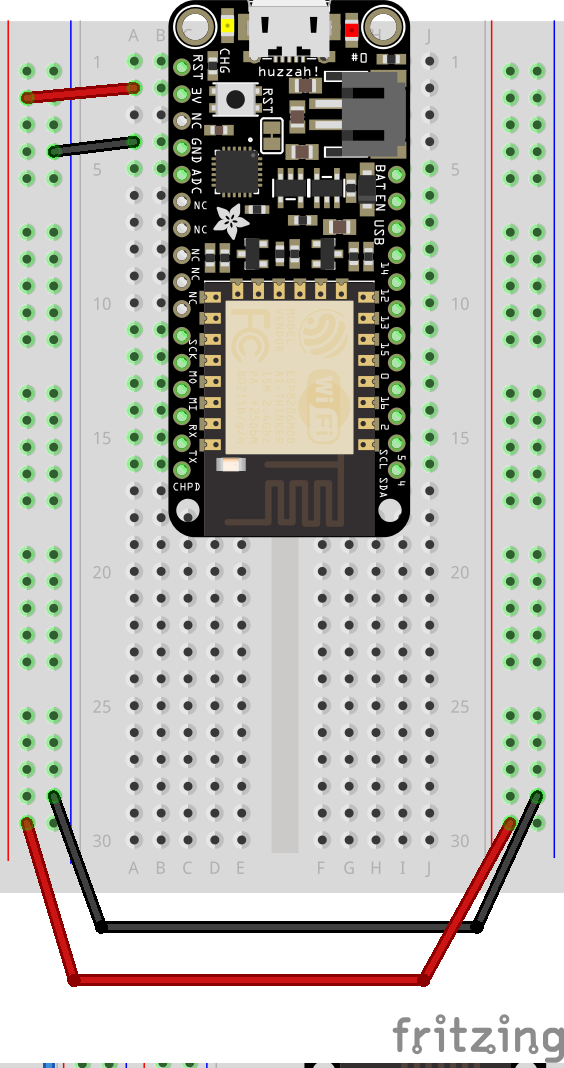
\includegraphics[width=\MFW]{Fritzing/feather_rails.png}}{https://publicsensors.org/IntroSensors/Fritzing/feather_rails.png}
		\caption[Power/ground rails connection schematic]{Typical layout for connecting power and ground rails to a Feather microcontroller.}
		\labfig{feather_rails}
	\end{center}
\end{marginfigure}

\subsubsection{\howto Construct a power distribution sub-circuit}
\begin{enumerate}
	\item \textbf{Disconnect your ESP8266 from the USB cable}.
	
	It is usually wise to turn off power to the microcontroller while you assemble circuits. 
	Otherwise, misplacing a jumper, or even briefly brushing it against the microcontroller or another component, can cause a short circuit and permanently damage your microcontroller! 
 	
 	Because the USB cable automatically supplies power, the only way to turn off power to the microcontroller is to disconnect the USB cable.
	When you're done assembling the circuit, check that the connections are as you intended before connecting again to USB power.  
	
	\item \textbf{Use a jumper to connect the \texttt{GND} pin on the ESP8266 to the negative (blue) rail}.
	
	To complete this step, note the pin labeled \texttt{GND} (for ``ground'', or \texttt{0 volts}) on the upper left side of the Feather in \reffig{margin_esp8266}. 
	One end of the jumper should be inserted into an open hole in the same row as the \texttt{GND} pin. 
	The other end should be inserted somewhere in the exterior column of holes immediately to the left (see \reffig{feather_rails}).
	
	\item \textbf{Use a longer jumper to connect the bottom hole in the left side negative rail to the bottom hole on the right side negative (blue) rail}. 
	
	Your jumpers should now look something like the black lines in \reffig{margin_breadboard_esp8266}. 
	In this configuration, any wire inserted into the negative rail on either side will be automatically connected to ground (\texttt{0 volts)}.
	
	\item \textbf{Connect the pin marked \texttt{3V} on the ESP8266 to the positive (red) power rail.}
	
	The \texttt{3V} pin, on the upper left side of the Feather, supplies a constant 3.3 volts from a voltage regulator (there is not enough room on the board to write the second decimal place!).	
%	The \texttt{USB} pin, located on the upper right side of the microcontroller, is connected internally to the USB power supply. 
%	USB power is always supplied at \texttt{+5 volts}. 
%	Use another jumper to connect an empty hole in the same row as the \texttt{USB} pin to any hole in the right side positive rail.
	
	\item \textbf{Use a longer jumper to connect the bottom hole in the left side positive rail to the bottom hole on the right side positive rail}. 
	
	Now, any wire inserted into the positive rail on either side will be automatically connected to \texttt{3.3 volts}.
	
	%The power rails are the two outermost sets of pins, arranged in columns running the length of the breadboard. These make electrical power easily available to devices connected to the power rails.
	\item \textbf{Check your circuit}.

	Make sure that, in the circuit you assembled: the left positive rail is connected to the \texttt{3V} pin, the right positive rail is connected to the left positive rail, the left negative rail is connected to the \texttt{GND} pin, and the right negative rail is connected to the left negative rail.
	
	\emph{Confirm that at no point does a jumper connect the positive part of the circuit directly to a negative part of the circuit.}

	\item \textbf{Plug your USB cable back into the microcontroller}.
	
	Use a multimeter to test your circuit, making sure it works correctly. 
	An easy way to do this is to use insert one end of a male-male jumper into one of the positive rails. 
	Insert one end of \textbf{another} male-male jumper into one of the negative rails. 
	Now, use the multimeter to test the voltage difference between the free ends of the two jumpers.
	\sidenote[][*-4]{\begin{kaobox}[backgroundcolor=\SNcolor,frametitlebackgroundcolor=\SNcolor,frametitle=CAREFUL!]Make sure not to connect the positive and negative rails directly together --- for example by brushing the leads of the multimeter to each other while they are touching the rails. This would cause a short circuit that could damage your microcontroller!\end{kaobox}}
	
\end{enumerate}
\loadMilestone{mlst:02b} % load milestone with tags id: mlst:02b

\subsection{GPIO as inputs: Responding to button pushes}
One of the most useful things a GPIO does is let you control your microcontroller through external devices like switches. 
For example, in an environmental sensor, you might want to turn sampling on and off with a button switch, have nearby motion trigger a camera, or count rotations of a propeller to measure wind speed. All of these involve using GPIOs as inputs. 

As a first step, you will assemble a sub-circuit enabling the microcontroller to respond to button presses
\sidenote[][*-12]{\begin{kaobox}[backgroundcolor=\SNcolor,frametitlebackgroundcolor=\SNcolor,frametitle=Button it up!]
	The type of switch used in this circuit is called a \emph{momentary} switch. 
	``Momentary'' means the switch will connect two pins while the button is being pressed, and immediately disconnect them when the button is released. 
	Many other types of switches are available for different functions. 
	For example, some switches \emph{toggle}: they form a connection when a button is pressed, and don't disconnect until the next time the button is pressed. Other types of switches are turned off by light, magnetic fields, or electrical signals instead of buttons.
\end{kaobox}}. A typical sub-circuit enabling a microcontroller to respond to button pushes is illustrated in \reffig{feather_switch}. 
This sub-circuit will require a button switch and two jumpers, and a few lines of code. 
When this sub-circuit works properly, you'll incorporate it into the other components of the circuit so that a button push starts and stops LED snoozing. 

Some button switches have two pins. 
With these switches, the two pins should go into different rows on the breadboard.
Pressing the button then forms an electrical connection between those two rows.

Like many other button switches, the switch in this illustration one has four pins. 
This is mostly for mechanical support, to keep the pins from breaking or pulling out too easily.
Two pairs of these pins are connected to each other, so there are really just two independent sets of pins that are connected and disconnected by button presses.

Notice that the pins are not equally spaced. 
The different spacing is to help you orient the button correctly.
 
On two opposite edges, pins are spaced to span over \emph{three} holes on a breadboard. 
We will call these the \emph{wide} sides.
On this type of button, the wide side pins are permanently connected to each other, inside the switch. \sidenote[][*-10]{\begin{kaobox}[backgroundcolor=\SNcolor,frametitlebackgroundcolor=\SNcolor,frametitle=This turns me on!]
	Sometimes it's hard to tell which orientation a 4-pin button should be plugged into a breadboard. In most breadboard layouts, a button's wide side pins are placed in the same row on the same side of the gutter as in \reffig{feather_switch}. 
	Occasionally, though, the wide side pins are placed on opposite sides of the gutter, in which case they act as a jumper connecting adjacent rows across the gutter. 
	In this configuration, pressing the button connects all four breadboard rows (two on each side of the gutter)!\end{kaobox}}

On the perpendicular edges, pins are spaced to span over \emph{two} holes on a breadboard. 
We will call these the \emph{narrow} sides.
The narrow side pins are insulated from each other, unless the button is pushed. 
While the button is being held down, a connection is made across the narrow sides.
When the button is released, the narrow side pins are again insulated from each other.

\subsubsection{\howto Assemble a button switch sub-circuit}
\begin{enumerate}
	\item  \textbf{Check your button with a multimeter, to find out which pins are connected when the button is in its pressed and unpressed state. }
	
	Most multimeters have a setting for measuring resistance, often marked by a $\Omega$ symbol. 
	This can be used for testing which pins on a button are connected to each other: 
	An ``open line'' (no connection) is indicated by a \texttt{OL}; a closed connection is indicated by a resistance at or near \texttt{0}. 
	Some multimeters also have a setting specifically for measuring \texttt{continuity}, and can trigger a beeping or buzzing sound when a connection is made. 
	
	\smallskip
	The easiest way to test a button is to insert it into a breadboard, and insert two male-male jumpers into the rows in line with the pins. 
	Then, use the multimeter to test continuity between the open ends of the two jumpers.  
	If the button is in the right orientation, the jumpers will be connected when the botton is pressed, but not when the button is released.
	
	\item  \textbf{Connect your button to the breadboard.}

	As shown in \reffig{feather_switch}, make sure the wide sides are aligned with a row. 
	As usual, the exact rows in which the button is placed are not critical. 
	However, it's a good idea to place the button reasonably close to the bottom of the microcontroller, so there is enough room to assemble other sub-circuits.
	
	\begin{marginfigure}[-5cm]
		\begin{center}
			\htmladdnormallink{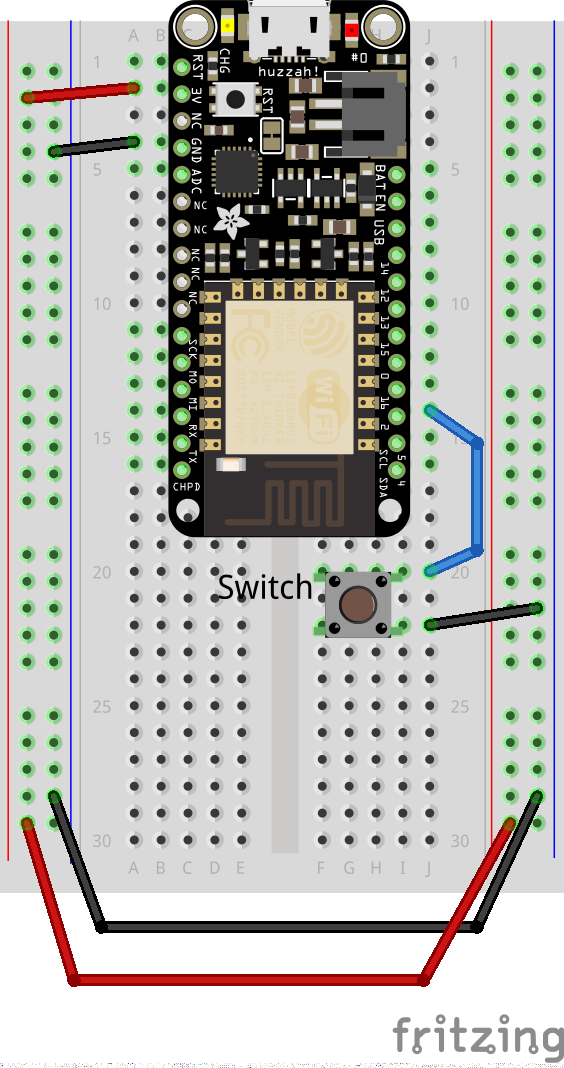
\includegraphics[width=\MFW]{Fritzing/feather_switch.png}}{https://publicsensors.org/IntroSensors/Fritzing/feather_switch.png}
			\caption[Button connections schematic]{An illustration of the layout for connecting a button switch to an input GPIO on the Feather. 
				Notice the orientation of the button: 
				For this kind of button, the more widely spaced pins orient along rows, and the more narrowly spaced pins orient along columns. 
				For other types of buttons, the exact placement may vary a bit.}
			\labfig{feather_switch}
		\end{center}
	\end{marginfigure}

	\item  \textbf{Jumper one wide side pin pair to the negative rail.}
	
	Because all the holes in the negative rail are connected to each other, any of them will work for our purposes. This means we're free to choose a hole that makes our sub-circuit compact and neat, and out of the way of other sub-circuits. 

	\item  \textbf{Jumper the other wide side pin pair to \texttt{Pin 2}.}
	
	Any of the numbered pins can act as input GPIOs. By choosing \texttt{Pin 2}, we will be able to see the effect of our button via the on-board red LED.
	
%\end{enumerate}
%That's it for the hardware. 

%Now we need to import the Pin method, define \texttt{GPIO 2} as an input pin, and test whether our button sub-circuit works as intended:
	\item \textbf{Import the Pin method, and define \texttt{GPIO 2} as an input pin.}
\begin{lstlisting}[language=Python]
from machine import Pin 
pin2 = Pin(2, Pin.IN,pull=Pin.PULL_UP) 
\end{lstlisting}	
	In the call to the \texttt{Pin} method, the \texttt{pull=Pin.PULL\_UP} tells the microcontroller that its default value should be ``high'' (\texttt{3.3V}). When the button is pressed, \texttt{GPIO 2} is connected (through the switch and negative rail) to \texttt{GND} (\texttt{0V}). This changes \texttt{GPIO 2} from ``high'' to ``low''.

%\begin{itemize}
	\item \textbf{Test the sub-circuit.}
	
	When you press the button, you should see a change in the state of the blue LED indicating \texttt{GPIO 2} changed from ``high'' to ``low''. 
	When you release the button, it should revert to its default state. 
	
	You can directly query the state of \texttt{GPIO 2} with the command
\begin{lstlisting}[language=Python]
pin2.value() 
\end{lstlisting}	
	Try it, to confirm that \texttt{GPIO 2} turns from value 1 (\texttt{3.3V}) to value 0 (\texttt{0V}) while you press the button, and reverts to value 1 when you release it.
	
\end{enumerate}
Does this happen? 
If so, congratulations, you've made a functional button input! 
If not, examine each of the component placements on the breadboard, and each line of MicroPython code you executed. 
When you find the difference between what you did and what you meant to do, the sub-circuit will be fixed.
\loadMilestone{mlst:02c} % load milestone with tags id: mlst:02c

\subsection{Acting reflexively: GPIO \texttt{interrupts} and \texttt{handlers}}
Now that you have a button that conveys a signal to your microcontroller, how can you use it to perform a useful function? 
One approach would be to have a code that continually checks whether a button is being pressed or not. 
However, this wastes a lot of processing power, and besides is cumbersome to incorporate into environmental sensor codes.

Like most modern microcontrollers, \texttt{ESP8266}s can be programmed to have ``reflexes'', which cause them to automatically perform a task when a specific GPIO changes between its ``high'' and ``low'' states. 
These reflexes are called \emph{interrupts}, because (with some exceptions) they can be triggered even when the microcontroller is busy running a MicroPython script to perform another task. 

There are two steps to defining a GPIO \texttt{interrupt}:
\begin{enumerate}
	\item Instruct the microcontroller what you want to happen as a response when a GPIO shifts from ``high'' to ``low'', or from ``low'' to ``high'' (these can have different responses). 
	These instructions takes the form of a Python method, called a \emph{handler}. 
	
	\item Program one of the GPIOs to execute that \texttt{handler} when its state changes.

\end{enumerate}
These steps are best explained with an example. 

\subsubsection{\howto Program an interrupt responding to button presses}
Suppose we would like to set up our microcontroller so that, when we press the button, it \emph{toggles} the red LED (that is, it alternately switches \texttt{Pin 0} on and off). \verb|button_interrupt.py| is an example of code giving this behavior using our button sub-circuit:
\begin{enumerate}
	\item \textbf{Download the} \lstinline{button_interrupt.py} \textbf{python script, and copy it onto your microcontroller.}
	\lstinputlisting[language=Python,label=ButtonInterrupt,caption={\htmladdnormallink{\texttt{button\textunderscore interrupt.py}}{https://github.com/publicsensors/IntroSensors/blob/main/Codes/button_interrupt.py}: A Micropython script to toggle the state of GPIO 2 when GPIO 0 changes state.}]{Codes/button_interrupt.py}
	In this code, \lstinline{togglePin0} is the ``handler'' -- it is the function that will get called when the interrupt is triggered. 
	The ``irq'' in the \lstinline{pin2.irq} command stands for ``interrupt request'' -- this is the command that tells the microcontroller to execute the handler function in response to a change in the state of \lstinline{pin2}. 
	
	\item \textbf{In a \texttt{REPL} session, import the module:}
\begin{lstlisting}[language=Python]
import buttonInterrupt
\end{lstlisting}	
	Now, in addition to the direct action of the button (changing the state of the blue LED), it also triggers an \texttt{interrupt} that changes the state of the red LED.
	\item \textbf{Optionally, replace the} \lstinline{pin2.irq} \textbf{command by uncommenting one of the alternatives below it.}
		
	\texttt{GPIO} \texttt{interrupts} respond to pin state transitions high$\rightarrow$low as different types of events from low$\rightarrow$high transitions.
	In coding an \texttt{interrupt}, you can specify responses to either or both of these transitions.
	
	\smallskip
	The code gives three alternative versions of the \lstinline{pin2.irq} command.
	The first version tells the microcontroller to execute \lstinline{togglePin0} only when \lstinline{pin2.value()} ``falls'' -- that is, goes high $\rightarrow$ low. 
	The second version, which is commented out in the example, tells the microcontroller to execute \lstinline{togglePin0} only when \lstinline{pin2.value()} ``rises'' -- that is, goes low $\rightarrow$ high. 
	The third version, which is also commented out in the example, tells the microcontroller to execute \lstinline{togglePin0} when \lstinline{pin2.value()} changes, either rising or falling.
	In different environmental sensing applications, different choices among these behaviors might be the most useful. 

	\smallskip
	How does your circuit behave if you use \lstinline{trigger=Pin.IRQ_FALLING|Pin.IRQ_RISING} to define your \texttt{interrupt}, so it responds to both high$\rightarrow$low and low$\rightarrow$high state changes?
\end{enumerate}
\loadMilestone{mlst:02d} % load milestone with tags id: mlst:02b



\subsection{Controlling external devices using your microcontroller.}
Now that you have some familiarity with \texttt{GPIO}s, and have the power distribution sub-circuit set up on your breadboard, you are ready to build a sub-circuit to power and control an external LED. 
Because this sub-circuit is a little more complex, we will construct it in parts --- ``sub-sub-circuits'' --- that are simpler to assemble, test, and if necessary debug.
There are three of these parts: powering an external LED; installing a relay to control the LED; and, programming an interrupt to switch the relay on and off.
\subsubsection{\howto Power an external LED}
\labsec{ext_led}
We'll begin by wiring an LED into the existing components on your breadboard. 
\reffig{feather_switch_LED} illustrates the layout of the sub-circuit you're about to build.
As usual, there is some flexibility about exactly which hole and which row a wire is placed. 
However, it's a good idea to look over \reffig{feather_switch_relay_LED} to see where additional components will be placed, and to leave space for those.
Placing components similarly to \reffig{feather_switch_LED} is one way to do that. 
\begin{marginfigure}[-8cm]
	\begin{center}
		\htmladdnormallink{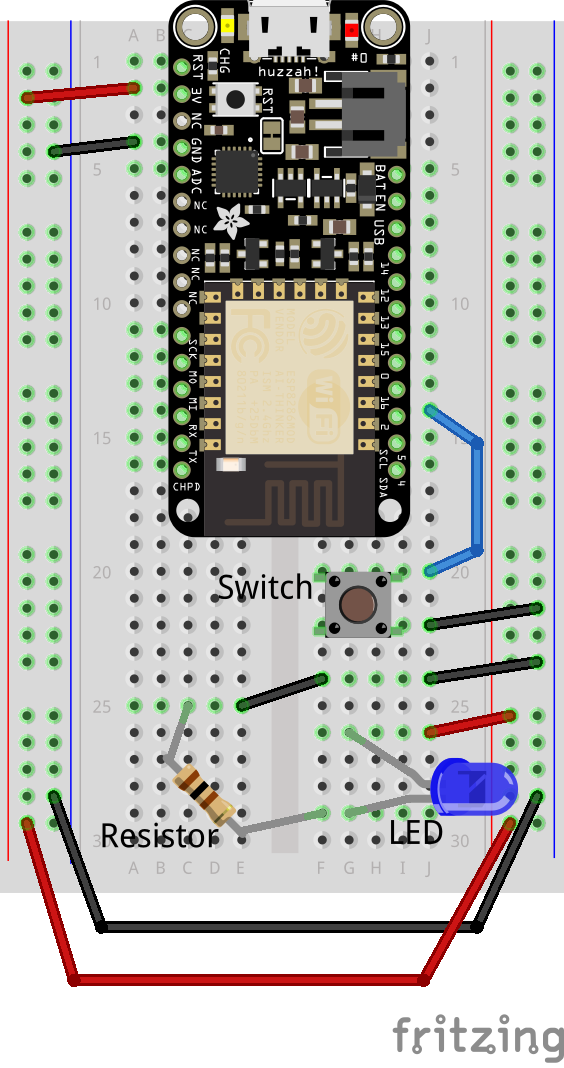
\includegraphics[width=\MFW]{Fritzing/feather_switch_LED.png}}{https://publicsensors.org/IntroSensors/Fritzing/feather_switch_LED.png}
		\caption[External LED layout]{An illustration of the layout for an external LED. }
		\labfig{feather_switch_LED}
	\end{center}
\end{marginfigure}


\begin{enumerate}
	\item \textbf{Connect a jumper from the negative rail on the right side of the breadboard, to the rightmost hole in a row slightly below the button.}
	\item \textbf{Connect a jumper from the leftmost hole in this row, across the gutter to one row lower.}
	
	This jumper placement will make it easy to substitute a relay for the jumper later on. 
	\item \textbf{Using a 100 Ohm resistor\sidenote[][*-3]{
			\begin{kaobox}[backgroundcolor=\SNcolor,frametitlebackgroundcolor=\SNcolor,frametitle=Pi\`ece de r\'esistance]
				Depending on which type of LED you use, you may need to modify the value of this resistor. 
				In \refch{circuits_intro}, you will learn how to calculate appropriate resistor values if you use a different type of LED than the one suggested here (though many types are close enough to work with the suggested resistor). 
				In the meantime, you can use an online   \htmladdnormallink{LED Resistor Calculator}{http://www.ohmslawcalculator.com/led-resistor-calculator} to figure out which resistor you need.
			\end{kaobox}
		}: Connect one wire to the left end of that jumper, and the other end into a row somewhere on the right side of the gutter.} 
	
	It does not matter which end of the resistor you start with, because resistors function the same way in either direction. 
	The exact row you connect to on the right side of the gutter also doesn't matter --- you are free to use any row as long as it is empty, and it's reasonably convenient to connect with jumpers to the other components in the circuit. 
	If you are unsure, pick a row and see how it works. 
	If connections later seem awkward or confusing, it's easy to move components to different rows to make the circuit smaller and neater.
	
	
	
	\item \textbf{Connect your LED into your circuit.}
	
	On your LED, notice that the two wires are of different lengths. The longer wire on an LED is always the positive side, and the shorter wire is the negative side. Connect the negative (shorter) LED wire to another hole in the same row as the resistor. Now connect the positive (longer) wire on the LED to an empty row. 
	
	\item \textbf{Connect the row with the positive wire from the LED to any hole in the positive (red) power rail.}
	
	\item \textbf{Check your circuit}.
	
	Confirm that, in the circuit you assembled: the LED is electrically connected on its positive terminal to 3.3 \texttt{volts} from the ESP8266; and, on its negative side, the LED is connected to the resistor, which in turn is connected to GND.
	
	\item \textbf{Plug your USB cable back into the microcontroller}.
\end{enumerate}
Does the LED light up? If so --- congratulations, you’ve made a working circuit! 
If not, check carefully that each of the connections was exactly what you intended, and that the positive and negative wires on the LED are in the appropriate holes. 
It’s easy to make small mistakes, but usually also easy to correct them!
\loadMilestone{mlst:02e} % load milestone with tags id: mlst:02e


\subsubsection{\howto Switch the LED with a relay}

Having built a circuit to power an external LED, you are now ready to enhance that circuit to enable your ESP8266 to control the LED.
To accomplish this, you will create a circuit using a \emph{relay}.

A relay is a switch that is controlled by an electrical signal. 
Relays help overcome a basic limitation of microcontrollers: they can supply only low levels of voltage and current. 
How, then, can a microcontroller control a device that requires large voltages or currents?
By switching on and off an external power supply (which may be high voltage or current), relays enable your ESP8266 to control external devices, even ones that require far more current or voltage than the microcontroller can supply directly.

The relay in the circuit you build in this example will control only a small device (an LED).
However, the same circuit configuration with a larger power supply and more robust relay could be used to control large equipment like winches, pumps, light banks, \etc that use large amounts of current or high voltages. 


\begin{marginfigure}[-0cm]
	\begin{center}
		\htmladdnormallink{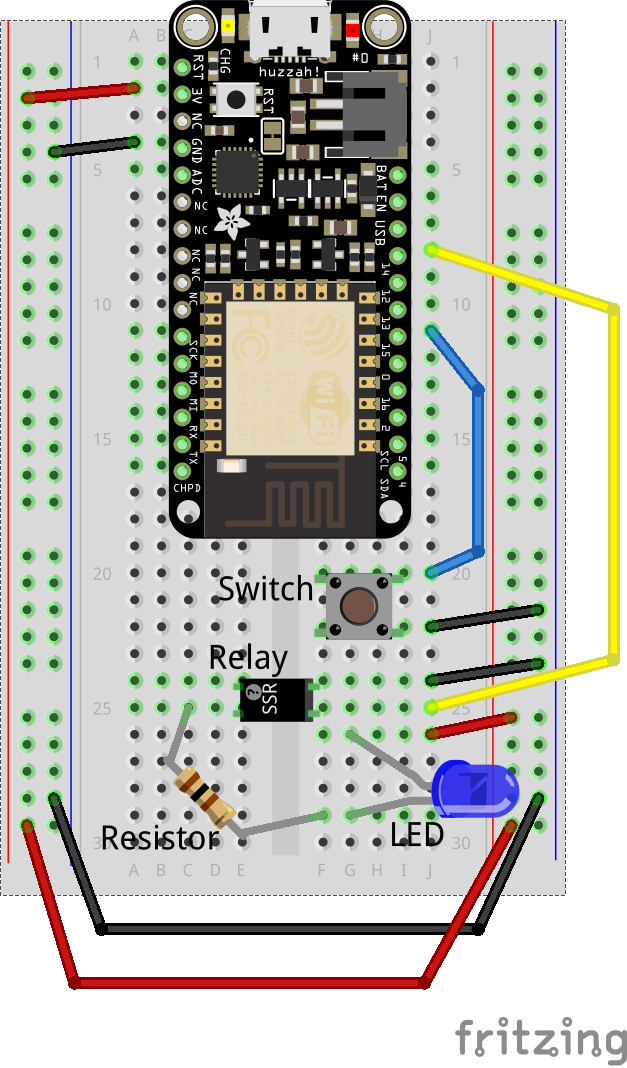
\includegraphics[width=\MFW]{Fritzing/feather_switch_relay_LED.png}}{https://publicsensors.org/IntroSensors/Fritzing/feather_switch_relay_LED.png}
		\caption[Button/external LED layout]{An example of layout for the relay-LED sub-circuit. }
		\labfig{feather_switch_relay_LED}
	\end{center}
\end{marginfigure}

%The figure is: \reffig{feather_switch_relay_LED}

%\begin{marginfigure}[5cm]
%	\includegraphics{Images/LEDrelay_circuitESP8266feather.jpg}
%	\caption[ESP8266 LED relay circuit]{A circuit in which an ESP8266 Feather microcontroller switches an LED using a relay.}
%	\labfig{margin_LEDrelay_esp8266}
%\end{marginfigure}

As you build your circuit, refer to \reffig{feather_switch_relay_LED} %\reffig{margin_LEDrelay_esp8266}
 for guidance:

\begin{enumerate}
	\item \textbf{Disconnect your ESP8266 from the USB cable}.

	\item \textbf{Remove the jumper spanning across the gutter}. 
	
	\item \textbf{In its place, insert a relay into your breadboard, as shown in the illustration}.
	Make sure that: 
	\begin{itemize}
		\item[$\circ$] The relay spans across the ``gutter''; and
		\item[$\circ$] The relay is oriented so that the writing is rightside up (with the tops of letters closest to the ESP8266).
		
		\smallskip
		This may be easier with the aid of a magnifying glass. Note the pins are different on the two sides of the relay, making it easier to tell which side is which.
	\end{itemize}
	
	\item \textbf{Connect the upper right pin on the relay to the negative (blue) power rail.}
	
	\item \textbf{Connect the lower right pin on the relay to the hole next to pin 14 on the ESP8266.} 
	
	This is the GPIO pin you will use to control the relay (note the pin is a little above the label).
	
%	\item \textbf{Connect one wire of a 100 Ohm resistor to the upper left pin on the relay. Put the other end into a row somewhere below the relay (again, it does not matter exactly which one).}
%	
%	\item \textbf{Put the negative (short) wire of your LED into another hole in the same row as the resistor, on the same side of the gutter.}
%	
%	\item \textbf{Now, connect the positive (long) wire on the LED to the positive (red) power rail.}

	\item \textbf{Check your circuit.}	
	
	In particular, make sure that, on the left side of the gutter, the resistor is connected to the left side of the relay.

	\item \textbf{Plug your USB cable back into the microcontroller}.
\end{enumerate}

That’s it for the hardware! Now we need to do the software:

\begin{enumerate}[resume]
	\item \textbf{Initialize GPIO 14 as you did for pins 0 and 2 before, and toggle its value:}
\begin{lstlisting}[language=Python]
from machine import Pin
p14 = Pin(14, Pin.OUT)
p14.value()
p14.value(1)
p14.value()
p14.value(0)
\end{lstlisting}
\end{enumerate}
Did the GPIO control the external LED? If so – well done, you’ve used a relay to control a device! 
If not, look things over and see if you can find a flaw in the assembly of your circuit or the Python commands to control it.
\loadMilestone{mlst:02f} % load milestone with tags id: mlst:02f

\subsection{Fine control using Pulse Width Modulation}
The GPIO pins on your ESP8266 (and many other microcontrollers) can output only two values --- high (\texttt{3.3V}) and low (\texttt{0V}). 
That's great for devices that need to be fully on or fully off. 
However, in many cases it’s useful to have an intermediate -- ``partway on''. 
One way to approach this is known as \htmladdnormallink{Pulse Width Modulation}{https://en.wikipedia.org/wiki/Pulse-width_modulation} (\texttt{PWM}). 
In \texttt{PWM}, the GPIO output is switched between ``on'' and ``off'' states very quickly (e.g. 1000 times per second), but the total fraction of time spend in the ``on'' state is varied gradually between 0 and 1. 
In some uses, this works as a close approximation to being able to continuously adjust pin voltages between on and off.

Let’s test what this does with our LED circuit. 
This test does not require any hardware modifications. 
We just need to redefine GPIO 14 in the code, to be a \texttt{PWM} pin instead of a simple digital output pin.

\subsubsection{\howto Snoozing an external LED}
%To keep things simple, do a soft reboot by typing \texttt{<ctrl>-d}. 
\begin{enumerate}
	\item \textbf{Create a PWM object attached to \texttt{GPIO 14}, and test it to make sure it regulates the LED:}
	\begin{lstlisting}[language=Python]
	from machine import Pin, PWM  # import the necessary modules
	pwm14 = PWM(Pin(14))      # create PWM object for GPIO 14
	pwm14.freq()             # get current frequency
	pwm14.freq(1000)         # set frequency
	pwm14.duty()             # get current duty cycle
	pwm14.duty(400)          # set duty cycle
	\end{lstlisting}
	Did the intensity of the LED change? 
	If so, you've succeeded!
	If not, check the code and the wiring to see where the mistake is.
	\smallskip
	Try changing the \texttt{PWM} parameters to make the LED brighter and fainter: 
	\begin{lstlisting}[language=Python]
	pwm14.duty(700)  # set a higher duty cycle
	pwm14.duty(100)  # set a lower duty cycle
	\end{lstlisting}
	\item \textbf{Using the \texttt{<ctrl>-e}/\texttt{<ctrl>-d} technique (or by downloading for the link), copy and execute the following code on your microcontroller:}
	\lstinputlisting[language=Python,label=SnoozeLED,caption={\htmladdnormallink{\texttt{snoozeLED.py}}{https://github.com/publicsensors/IntroSensors/blob/main/Codes/snoozeLED.py}: A Micropython script to ``snooze'' an LED regulated by \texttt{GPIO 14}, using Pulse Width Modulation.}]{Codes/snoozeLED.py}
	
	This code defines a method that automatically changes the \texttt{duty} parameter to cycle between brighter and fainter LED settings. 
	To execute it, use:
	\begin{lstlisting}[language=Python]
	snooze_led(pin=14)
	\end{lstlisting}
\end{enumerate}
If your LED is now “snoozing” (gradually getting brighter and dimmer) then you’ve successfully implemented Pulse Width Modulation control through your relay.
\begin{enumerate}[resume]
	\item \textbf{Try different choices of the parameters \texttt{freq}, \texttt{delta}, \texttt{delay} and \texttt{verbose}, e.g.} 
	\begin{lstlisting}[language=Python]
	snooze_led(pin=14,delay=300,verbose=True)
	\end{lstlisting}
	Setting \lstinline{verbose=True} gives a printout of the current \texttt{PWM} settings for each cycle.
\end{enumerate}

Note that, as is, this code will run indefinitely until it is interrupted. 
To stop it, enter \texttt{<ctrl>-c} (which halts any running code in Python). 
%\sidenote[][*6]{
	\begin{kaobox}[frametitle=Asleep at the switch!]
		How does this code use a pin that can only take on/off values and make it appear to ``snooze'' by continuously varying LED brightness? 
		After importing necessary modules (lines 1-2), the code defines Pin 14 as a Pulse Width Modulation object, with ``frequency'' set to 1000. 
		This means the pin will alternate between \texttt{0 volts} and \texttt{3.3 volts} at 1000 Hz (1000 times per second). 
		The ``duty'' is initially set to 200. 
		This means that the pin will be in the ``on'' state for 200/1023 of the time (duty of 0 is fully off, and duty of 1023 is fully on). 
		Our eyes cannot resolve fluctuations that happen 1000 times per second, so we see the LED as if it were partially on.
		The code defines a loop (at the \texttt{while} command), in which the duty parameter is incremented by \texttt{delta} (=50). 
		The duty increases each pass through the loop, so the LED appears brighter. 
		However, when duty=1000, delta is reset to -50, so that duty decreases each pass through the loop and the LED gets dimmer. 
		When duty reaches 0, delta is rest to 50, so duty increases again. 
		This alternation between increasing and decreasing duty, in combination with the relay's control over power to the LED, is what gives the ``snoozing'' behavior in the LED's brightness. 
	\end{kaobox}
%}

%As an extra challenge, you could add code to make the code run for a specific length of time, and then stop by itself. 
%If you take up this challenge, you may find it useful to discontinue the PWM, with
%\begin{lstlisting}[language=Python]
%pwm14.deinit()           # turn off PWM on the pin
%\end{lstlisting}
%at the end of your code.

%\section{Milestones}

%\begin{kaobox}[frametitle=Milestone 1]
%%	\begin{itemize}
%%		\item 
%		\loadMilestone{mlst:02} % load milestone with tags id: mlst:02
%%	\end{itemize}
%\end{kaobox}
\loadMilestone{mlst:02} % load milestone with tags id: mlst:02

%\todo{Add section using switch as an input to GPIO (e.g. to start and stop snoozing)?}
%\todo{Have notation to indicate advanced or optional sections?}
%\todo{Have indications of prerequisite earlier sections for later sections?}
%\todo{Convert all script to methods that can be rerun without importing?}
\todo{Recalculate resistor value for 3V3 instead of VUSB power}
%\todo{``We'' vs. ``you''.}
\todo{Set up a coding exercise, to use an interrupt derived from \texttt{button\_interrupt.py} to launch and halt execution of a modified version of \texttt{snoozeLED.py}.}


\setchapterstyle{kao}
\setchapterpreamble[u]{\margintoc}
\chapter{Keeping track of time: Accuracy and precision in Real Time Clocks}
\labch{time_keeping}

For taking sensor readings to measure environmental conditions, and for many other uses of microcontrollers, it’s often important to have a reliable measure of time. 
In some cases, the sensor data are themselves based on elapsed time.
For example, wind speed is often calculated from the time elapsed during rotations of the propeller on an anemometer. 
The period of ocean waves may be calculated from the elapsed time between peaks and troughs. 
More generally, even if a sensor reading does not depend directly on elapsed time, it is likely to be far more useful if it is combined with a timestamp recording when it was taken. 
This places it in the context of previous and subsequent readings, concurrent readings by other sensors, position within the track of a moving ship, and so on.


In this chapter, you will set up and assess three ways of determining time with your \texttt{ESP8266}:
\begin{enumerate}
	\item Using the on-board \texttt{Real Time Clock} (often abbreviated as \rtc). 
	Like most modern microcontrollers, the ESP8266 has a built-in \rtc, which a measurement of the current time available through MicroPython. 
	These are very convenient to use, but vary widely in their reliability.

	\item Using an \rtc mounted on an external circuit board, called a \DS3231, that communicates with your microcontroller via a digital protocol called \i2c.

	\item From the Internet, using a utility called \texttt{Network Time Protocol} (\ntp). 
	This utility is the way your desktop and laptop update their internal clocks to maintain accuracy. 
	Your microcontroller can do the same thing!
\end{enumerate}
Each of these time-keeping methods has an important role to play in environmental sensing. 
We will explore the advantages and disadvantages of each method partly in this chapter, and in more depth during construction and deployment of field instruments for environmental monitoring in \refch{instr_constr}.

\begin{table}[h]
	\caption[\refch{time_keeping} materials]{\textbf{Materials you'll need\dots} 
		
		See Table \ref{tab:materials} for additional information.}
	\labtab{materials_time_keeping}
	\begin{center}
		\raggedright
		%\begin{tabular}{ c c c c } 
		\begin{tabular}{ c r c}
			\hline
			Sections & item & link \\
			\hline
			\multirow{2}{4em}{\refsec{set_read_time}} 
			& breadboard & \ref{mat:bb} \\
			& ESP8266 ``Feather'' & \ref{mat:mc} \\
			& micro-USB cable & \ref{mat:usb_cbl} \\
			%		\hline
			%		\multirow{3}{4em}{\vrefsec{circuits}}  
			& male-male jumpers & \ref{mat:jmp_mm} \\ 
			& pliers & \ref{mat:plr} \\ 
			& DS3231 RTC & \ref{mat:RTC} \\ 
			\hline
		\end{tabular}
		
\end{center}\end{table}

\section{Accuracy and precision}
\labsec{acc_prec}
A key idea in this chapter is that no time-keeping device is perfect. 
All have at least \textit{some} errors. 
To choose the best method of keeping time, and to know how far off our references to time are likely to be, we need metrics to measure the errors associated with each method. 

The most important metrics for quantifying errors in time-keeping %(as well as in other sensors) 
are  \textbf{accuracy} and \textbf{precision}. 
In everyday language, we might use these terms more or less interchangeably.
In science, however, they have quite different meanings:

``Accuracy'' refers to a systematic \emph{bias} in measurements.
For example, we say a clock runs ``fast'' if it consistently reports more time having passed than the true time.
The clock runs ``slow'' if it consistently reports less time having passed than the true time.
Both of these errors reflect lack of accuracy -- this clock is, on average, \emph{biased} towards under- or over-estimating the true passage of time.

Under some circumstances, we might be able to increase accuracy with a \textbf{calibration}.
A calibration is a quantitative relationship between a measurement and a true physical parameter (in this case, time).

For example, if we know a clock runs fast by two minutes per day, we might calibrate that clock by calculating the ratio of the number of seconds in a day (60 seconds per hour $\times$ 60 minutes per hour $\times$ 24 hours per day) to the number of seconds reported by the clock (60 seconds per hour $\times$ 60 minutes per hour $\times$ 24 hours per day + 2 $\times$ 60):
\[ 
\frac{60 \times 60 \times 24}{60 \times 60 \times 24 + 2 \times 60 } = \frac{86400}{86520} = 0.99861
 \]
This calibration tells us that if we multiply the clock's measure of elapsed time by the factor 0.99861, we compensate for its biased tendency to run fast.
This adjusted time will be much more accurate than the clock's nominal time reading.

``Precision'' refers to the \emph{scatter} in a large number measurements of the same physical quantity. 
For example, if we use a stopwatch to repeatedly time an event that we know to take exactly one hour, one measurement might be 3595 seconds, the next might be 3605 seconds, and so on. 
These deviations among measurements (in this case, a difference of 10 seconds between successive measurements) represent lack of precision. 

Because these errors are random, or at least unpredictable, we cannot devise a calibration to mitigate them. 
However, under some circumstances, we might be able to take an average or median of many measurements. 
If so, the precision of this average or median is often much better than the precision of a single measurement.

It's important to recognize that accuracy and precision reflect distinct characteristics of a dataset. 
A set of measurements can be accurate but not precise, precise but not accurate, both precise and accurate, or both inaccurate and imprecise. 


\section{Setting and reading time on the ESP8266}
\labsec{set_read_time}
The exercises in this chapter have two parts. 
In this, the first part, you will set up and test the hardware and software needed to use the three methods of time-keeping. 
In the second part, you will assess the relative accuracy and precision of the on-board and external RTCs, relative to NTP (Internet) based time-keeping.

\subsection{The On-Board RTC}
Your ESP8266 microcontroller arrives from the factory with a clock already built into it and accessible through MicroPython codes. 
We will refer to this clock as the \emph{on-board RTC}, to distinguish it from other sources of time like external devices or the Internet.
Because the on-board RTC is already present on your microcontroller, it can be accessed without any additional hardware --- we need only execute a few Python commands. 

\subsubsection{\howto Read and set the on-board RTC}
To use the on-board RTC:
\begin{enumerate}
	\item \textbf{Import the \rtc method from the machine module and create an instance of the RTC class}:
	\begin{lstlisting}[language=Python]
	from machine import RTC
	rtc = RTC() 
	\end{lstlisting}
	Here, \lstinline{rtc} is the variable name for an instance of the \rtc object.
	\item \textbf{Query} \lstinline{rtc} \textbf{to obtain a time reading from the on-board \rtc}:
	\begin{lstlisting}[language=Python]
	rtc.datetime() # get date and time
	\end{lstlisting}
	The format of the output from this command is a Python \htmladdnormallink{tuple}{https://docs.python.org/3.3/tutorial/datastructures.html\#tuples-and-sequences}: \texttt{(year, month, day, weekday, hour, minute, second, microsecond)}.
	
	Note that the on-board \rtc initially has a default time that has no bearing on the actual time.
	\sidenote[][*-22]{\begin{kaobox}[backgroundcolor=\SNcolor,frametitlebackgroundcolor=\SNcolor,frametitle=Wrinkles in time\dots]The onboard \rtc is turned off whenever the power is shut off to the ESP8266. That means if you unplug your ESP8266 from the USB cable (and if there is no battery to keep it powered up) the on-board \rtc will be reset to its default time.
	You must then reset it to have the correct time.
	However, if you reboot the microcontroller while keeping power on, the onboard \rtc stays on and preserves the current time. The onboard \rtc also preserves the current time when it goes into ``deepsleep'' to save energy.\end{kaobox}} 
	  
	\item \textbf{Set the current time on the on-board RTC with the command}
	\begin{lstlisting}[language=Python]
	rtc.datetime((2017, 8, 23, 1, 12, 48, 0, 0)) # set a specific date and time
	\end{lstlisting}
	In this example, the year is 2017, month is August (the 8th month), day is 23, weekday is 1, hour is 12, minute is 48, second is 0, and microsecond is 0. Try it (ideally with a more nearly correct time!) and check to make sure the time has been reset according to your command.
\end{enumerate}

Further information about using the on-board RTC can be found at Micropython.org's \htmladdnormallink{Quick Reference}{
http://docs.micropython.org/en/latest/esp8266/esp8266/quickref.html} and
\htmladdnormallink{Code Library}{http://docs.micropython.org/en/latest/esp8266/library/machine.RTC.html} documentation.

\subsection{Network Time Protocol (NTP)}
As you likely noticed in the previous step, it is difficult to set the on-board RTC from the command line with high accuracy. 
A more convenient and accurate way to set the clock is to use an online time source.
A human-readable example is the \htmladdnormallink{official time source}{https://www.time.gov/} for the U.S. government, operated by the National Institute of Standards and Technology (NIST).

For computers and microcontrollers, online time sources are easier to use with a machine-readable format called  
 \texttt{Network Time Protocol}, or \texttt{NTP}. 
An \texttt{NTP} server is an online portal using this protocol that enables a local machine to calculate the current time.  
Micropython has a built-in utility called \lstinline{ntptime} to automatically obtain the current time from an NTP server (the default is \texttt{pool.ntp.org}), if it is connected to the Internet via WiFi. 
\lstinline{ntptime} can also reset the on-board \rtc, to match the time from the NTP server. \todo{Create a box or hyperlink to the explanation of how NTP works.}
%We’ve provided a modified version of this utility, which can also be used in the next step to reset the external RTC.

%\marginnote{NOTE: 
	This part of the exercise assumes that your ESP8266 is connected via WiFi in \texttt{Station mode} to the Internet. If it is not, follow the instructions in \refsec{wifi_sta} to establish this WiFi connection, then continue with the exercise.
%} 

\subsubsection{\howto Obtain current time from the Internet}
To use an online NTP server to set the on-board \rtc to the current time:
\begin{enumerate}
	\item \textbf{Use} \lstinline{ntptime} \textbf{to get the current time from the NTP server with the commands}:
\begin{lstlisting}[language=Python]
import ntptime, utime
t=ntptime.time()
print('The result of ntptime.time() is: ',t)
print("Converted to human-readable time that's: ",utime.localtime(t))
\end{lstlisting}
	Note that the results of \lstinline{}
	\item \textbf{Set the time on the \texttt{ESP8266}’s internal RTC}:
\begin{lstlisting}[language=Python]
ntptime.settime()
\end{lstlisting}
	This command automatically retrieves the current time from the NTP server, and uses it to set time on the on-board RTC.
	\item \textbf{Query the on-board \rtc to verify the correct time has been set}:
\begin{lstlisting}[language=Python]
rtc.datetime() # get date and time
\end{lstlisting}
	You should see that the time has been set quite accurately to \texttt{Coordinated Universal Time} (\texttt{UTC}). 
\end{enumerate}


\subsection{DS3231 (external) RTC}
Our third method of keeping time is using an external RTC, known as a \DS3231.
The \DS3231 is an \rtc similar the ESP8266's \rtc, but with two important differences. 
One is that the \DS3231 has a coin cell battery.
This means that it keeps track of time, even when the microcontroller to which it's attached is powered down.
The other is that the \DS3231 is a specialized device, that performs only time-related functions. 
In \refsec{rel_acc}, we'll assess the accuracy and precision of this specialized time-keeping device compared to the ESP8266's onboard \rtc.

The \DS3231 interacts with a microcontroller using a \texttt{digital} protocol known as \i2c. 
The \i2c protocol is discussed in detail in \refch{telem_sens_coms}.
For now, the attribute of the \i2c interface we're most interested in is that it's very easy to set up. 
Connecting the \DS3231 external \rtc to your microcontroller requires just a few jumpers. 


\subsubsection{\howto Set up an external \rtc}




As you set up your circuit, refer to the example layout in \reffig{ds3231_breadboard}. 
Because there is only one component in this exercise, you have a lot of flexibility where to place your components and jumpers.
\begin{marginfigure}
	\begin{center}
		\htmladdnormallink{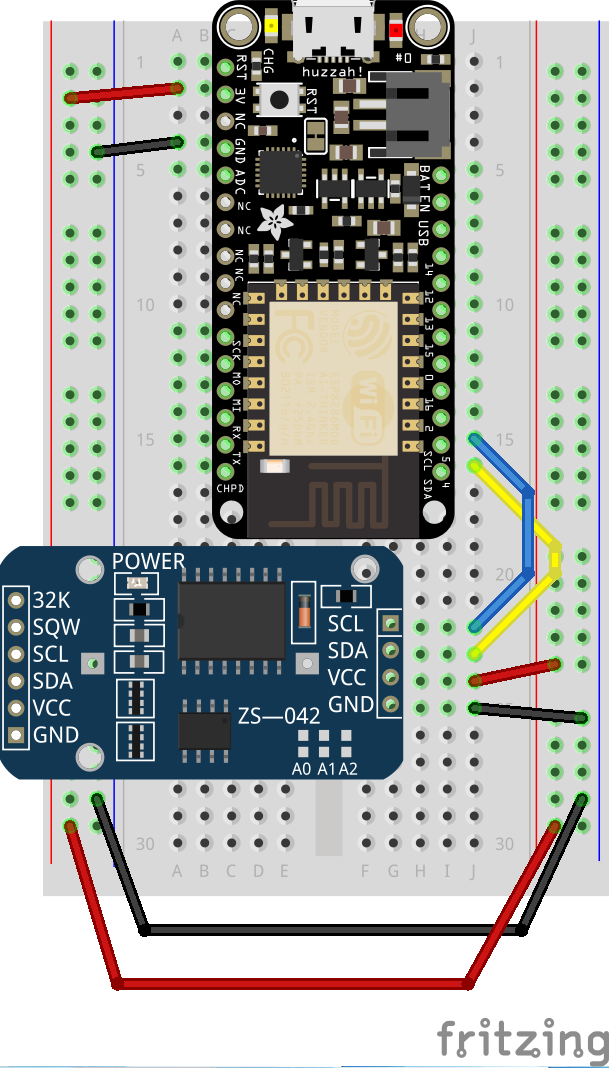
\includegraphics[width=\MFW]{Fritzing/feather_DS3231.png}}{https://publicsensors.org/IntroSensors/Fritzing/feather_DS3231.png}
		%\includegraphics[height=5cm]{Images/DS3231breadboard.jpg}
		\caption[DS3231 on breadboard]{An example of layout and wire connections for the DS3231 external Real Time Clock and ESP8266 microcontroller.}
		\labfig{ds3231_breadboard}
	\end{center}
\end{marginfigure}
\begin{enumerate}
	\item \textbf{Insert the coin cell battery into the battery holder (if it is not already in) with the positive (+) side out.}
	\item \textbf{Connect the GND and 3V pins on the ESP8266 to the GND and Vcc pins on the DS3231}. 
	
	You can do that directly with long jumpers, or (more neatly) using the positive and negative rails with short jumpers as in \reffig{ds3231_breadboard}.
	\item Connect the \texttt{SDA} (\#4) pin on the ESP8266 to the \texttt{SDA} pin on the \DS3231, and the  \texttt{SCL} (\#5) pin on the ESP8266 to \texttt{SCL} on the \DS3231.
	\item \textbf{Download the driver module provided by Adafruit called \htmladdnormallink{urtc.py}{https://github.com/adafruit/Adafruit-uRTC} for the \DS3231 \rtc.}
	
	Save it into a \texttt{Codes} directory on your computer.
	
	\item \textbf{Copy } \lstinline{urtc.py} \textbf{onto our microcontroller, using either the \texttt{WebREPL} or \mpfshell methods from \refch{connect}.}  
	\item %You are now ready to test your \DS3231 \rtc. 
	\textbf{Set up the \i2c connection to your \DS3231:}
\begin{lstlisting}[language=Python]
import urtc
from machine import I2C, Pin
i2c=I2C(scl=Pin(5),sda=Pin(4))
rtc3231=urtc.DS3231(i2c)
\end{lstlisting}
	\item Query the time from your \DS3231, with:
\begin{lstlisting}[language=Python]
rtc3231.datetime()  # print out current date/time tuple
datetime = rtc3231.datetime() 
print(datetime.year)          # Or, print out separate elements
print(datetime.month)         # of the date/time tuple
print(datetime.day)
print(datetime.weekday)
print(datetime.hour)
print(datetime.second)
\end{lstlisting}
\end{enumerate}

To set the time on the \DS3231 using the \ntp server, the easiest method is to use the following utility, called \texttt{SetTimeDS3231.py}:
\lstinputlisting[language=Python,label=SetTimeDS3231,caption={\htmladdnormallink{\texttt{SetTimeDS3231.py}}{https://publicsensors.org/IntroSensors/Codes/SetTimeDS3231.py}: A Micropython utility to set a \DS3231 \rtc to time from a Network Time Protocol (NTP) server.}]{Codes/SetTimeDS3231.py}
%\lstinputlisting[language=Python]{Codes/settimeDS3231.py}
\begin{enumerate}[resume]
	\item \textbf{Download} \lstinline{SetTimeDS3231.py}\textbf{, copy it onto your microcontroller, and execute:} 
\begin{lstlisting}[language=Python]
from SetTimeDS3231 import settimeDS3231
datetime = rtc3231.datetime()  # obtain and print the pre-existing time
print(datetime)                
settimeDS3231()                # set the DS3231 with NTP
datetime = rtc3231.datetime()  # obtain and print the
print(datetime)                # NTP-set time
\end{lstlisting}
	Try it and confirm that the time on the \DS3231 \rtc has been set correctly. 	
\end{enumerate}

You can also set your on-board \rtc from the \DS3231 by pasting (with \texttt{<ctrl>-e}/\texttt{<ctrl>-d} and executing the following two lines:
\begin{lstlisting}[language=Python]
tDS3231=rtc3231.datetime()
rtc.datetime((tDS3231.year,tDS3231.month,tDS3231.day,0,tDS3231.hour,tDS3231.minute,tDS3231.second,0))
\end{lstlisting}

More information about the \DS3231 \rtc can be found at \htmladdnormallink{http://micropython-urtc.readthedocs.io/en/latest/}{http://micropython-urtc.readthedocs.io/en/latest/}.

\loadMilestone{mlst:03} % load milestone with tags id: mlst:02


\section{Accuracy and precision of time-keeping on the ESP8266}
\labsec{rel_acc}
Now that your ESP8266 is set up to use all three methods to obtain the current time, we can consider how to use them most effectively for environmental sensing. 

Some considerations involve practical constraints. 
For example, in many field deployments of environmental sensors WiFi is either unavailable or available only intermittently, such as when a cell phone is used to create a temporary hotspot.
This constrains when \ntp is a viable option.
To save battery power, a microcontroller in an environmental sensor often puts itself to ``sleep'', waking up only briefly at preset intervals to take measurements.  
This wake-up function usually operates through the on-board \rtc, so this device must be used in at least some aspects of time-keeping. 

Other considerations involve the \emph{quality} of the temporal data from each of the three sources. % --- that is, their accuracy and precision. 
Because no time-keeping device is perfect, we expect that measurements of time intervals using any of these methods will result in a distribution of measured values, with varying deviations from the true values. 
The deviation of the center of this distribution from the true time corresponds to an \emph{accuracy} metric. 
The breadth of the distribution corresponds to a \emph{precision} metric. 
Together, accuracy and precision metrics enable us to anticipate how errors in time-keeping might accumulate during the deployment of an environmental sensor.

To decide how best to select among time-keeping methods for environmental sensing, we need to answer questions like: 
\begin{itemize}
	\item How big are the time-keeping errors for each method (that is, how accurate and precise are each of the methods)?
	\item Are particular \rtcs biased towards run fast or slow (that is, are some units ``defective'' so that they differ \emph{systematically} from the overall population of \rtcs)?
	\item Does the magnitude or direction of timekeeping error depend on environmental conditions (for example, do higher or lower temperatures affect time-keeping accuracy and precision)?  
\end{itemize}

To answer these questions objectively, we need two things:
\begin{itemize}
	\item A \emph{dataset} of simultaneous time measurements by different methods, that quantifies errors as relative differences in estimated time between methods; and,
	\item \emph{Statistical analysis} that enables us to visualize the error distributions, establish bounds for likely time-keeping deviations, and test hypotheses about performance of individual devices.
\end{itemize}
In this section, we will go step-by-step through the process of generating a dataset and analyzing it, to make inferences about time-keeping accuracy and precision. 
In addition to helping us devise a good strategy for tracking time for field sampling, these steps will be good preparation for generating and analyzing datasets from environmental sensors you will build and deploy in later chapters.


\subsection{Generating a dataset of time-keeping errors}
In generating data to characterize time-keeping, a few simplifications can greatly reduce the required effort. 
One of those is to consider only relative deviations among the on-board and \DS3231 \rtcs, compared to time from an \ntp server. 
This makes sense because \ntp servers are in general very accurate, and because we don't have an easily accessible alternative time source that is more accurate.
So, in effect, we will regard \ntp as giving the ``correct'' time.

Another simplification is to take time-keeping error samples over relatively short periods. 
On a deployment, an instrument might spend weeks or months without access to \ntp or any other means of correcting errors. 
Observing \rtcs over comparably long periods would give the most realistic assessment of time-keeping errors.
However, this is almost never practical during instrument design, assembly and testing.
We will therefore attempt to learn as much as possible using much shorter sampling periods.

\begin{kaobox}[frametitle=A download-able dataset of time-keeping errors]
	In a classroom setting with multiple microcontrollers and \rtcs (ideally 10 or more), generating your own dataset with the steps outlined below is the most informative strategy. 
	If you do not have access to a sufficient number of devices, or if you would like to focus on understanding the data analysis rather than acquiring new data, you can download an \htmladdnormallink{archived dataset}{https://publicsensors.org/IntroSensors/Codes/TimeDataExamples.zip} of time-keeping errors.
	This archive ``unzips'' to provide a directory called \lstinline{TimeData} containing 90 
	time-keeping error data files.
	You can use these files instead of your own dataset.
	
	\smallskip
	Alternatively, you can collect data for your own devices and compare them to the archived data. 
	However, to use the archived data in this way, you must use parameters for your data collection that are consistent with those use to generate the archive: 
	
	\lstinline{interval_sec=10*60, n_samples=12, n_replicates = 4}
%	\begin{lstlisting}[language=Python]
%	interval_sec=10*60
%	n_samples=12
%	n_replicates = 4
%	\end{lstlisting}
	
	As explained below, this corresponds to four replicates, each with 2-hour sequences of sampling at 10 minute intervals.
\end{kaobox}

\subsubsection{\howto Generate a time-keeping dataset}
To make generating a dataset easy, we’ve provided a Micropython function that automatically sets the on-board and \DS3231 \rtcs so that they initially agree with \texttt{NTP} time.
The function then records a sequence of time samples from each, and saves them to a data file.
This process is repeated a specified number of times, each time producing a new data file, to produce a replicated dataset. 

Follow these steps to generate your dataset:
\begin{enumerate}
	\item \textbf{Connect your microcontroller to \texttt{WiFi} in \texttt{STA} mode, so it can access the \texttt{NTP} server.}
	\item \textbf{Download the file} \todo{Include several passes through NTP connection because it's not always successful even if internet is available.} \htmladdnormallink{TimeCompare.py}{https://publicsensors.org/IntroSensors/Codes/TimeCompare.py}\textbf{ onto your computer, and use }\lstinline{mpfshell} \textbf{or} \lstinline{WebREPL} \textbf{to copy it onto your microcontroller.}
	\item \textbf{Initialize the on-board and external (\DS3231) \rtcs:}
\begin{lstlisting}[language=Python]
from machine import RTC
import urtc
from machine import I2C, Pin
from TimeCompare import time_compare
rtc_ = RTC()  # Initialize on-board RTC
i2c = I2C(scl=Pin(5), sda=Pin(4))  # Initialize DS3231 (external) RTC
rtc3231_=urtc.DS3231(i2c)
\end{lstlisting}
	Note the ``\textunderscore'' in some of the variable names. 
	This is to distinguish them from similar variable names in the Micropython function.
	\item \textbf{Define the sampling parameters, a modification of:}
\begin{lstlisting}[language=Python]
prefix_='danny'        # Filenames will start with this
interval_sec=10        #  Sampling interval, in seconds
#interval_sec=1*60     #  A format making it easy to specify intervals in minutes
#interval_sec=1*60*60  #  A format making it easy to specify intervals in hours
n_samples= 10      # Number of time intervals to sample
n_replicates = 3   # Number of times to replicate the sampling protocol
\end{lstlisting}
	The meaning of these parameters is:
	\begin{itemize}
		\item[$\circ$] \lstinline{prefix} is used to generate informative names for data files.
		
		\smallskip
		In this case, filenames will have the form \lstinline{danny_dda01900_568621029.txt} (starting with the prefix, \lstinline{danny}). 
		The prefix is followed by the unique ID of the microcontroller (\lstinline{dda01900}), then a timestamp (\lstinline{568621029}) recording when sampling starts, and finally a suffix (\lstinline{txt}) indicating the file type.
		
		\smallskip
		This convention gives filenames that are informative --- because of the prefix and microcontroller ID, they can be identified easily by both humans and machines.
		Also, because the timestamp does not repeat itself, no file can be accidentally overwritten by another file with the same name. 
		\item[$\circ$] \lstinline{interval_sec} is the parameter determining the length of intervals (in seconds) at which time samples should be taken.
		
		\smallskip
		This example illustrates two ``tricks'' that many Micropython users find helpful when collecting and analyzing data.
		\begin{itemize}
			\item[$\triangleright$] When sampling at longer intervals (e.g. 3.5 hours) to explicitly write \lstinline{3.5*60*60}. 
			This expression is much easier to understand at a glance than the same number multiplied out (\lstinline{12600.0}). 
			\item[$\triangleright$] When exploring parameter space, to comment out rather than delete previous values. 
			This makes it far easier to keep track of what you've already tried.			
		\end{itemize}		
		\item[$\circ$] \lstinline{n_samples} and \lstinline{n_replicates} specify, respectively, how many samples each data file should contain, and how many data files should be created. 
		
		\smallskip
		The total duration of sampling for each file will then be \lstinline{interval_sec} $\times$ \lstinline{n_samples} seconds. 
		Sampling for all the replicates will last \lstinline{interval_sec} $\times$ \lstinline{n_samples} $\times$ \lstinline{n_replicates} seconds.
	\end{itemize}
	\item \textbf{Execute a short sampling run, with the command:}
\begin{lstlisting}[language=Python]
time_compare(prefix=prefix_,rtc=rtc_,rtc3231=rtc3231_,interval_seconds=interval_sec,num_samples=n_samples,num_replicates=n_replicates)
\end{lstlisting}
	
	It's a good idea to first do some short test sampling runs, with parameters set so that the entire process will take just a couple minutes.
	The parameters above are an example of this. 
	If there is a problem with hardware or WiFi, these parameters enable you to detect that quickly.
	
	\item \textbf{Inspect the on-screen output.}
	
	The \lstinline{time_compare} function has two types of output. It writes output to the terminal, which looks like this:
\begin{lstlisting}[language=Python]
****Beginning replicate  1  ****

Trying to set the DS3231 RTC using NTP...
setting urtc datetime to:  DateTimeTuple(year=2020, month=1, day=15, weekday=None, hour=2, minute=2, second=56, millisecond=None)
...successfully set from NTP

Creating data file:  danny_c9865800_632368922.txt

sample_num,day_onboard,hour_onboard,min_onboard,sec_onboard,day_external,hour_external,min_external,sec_external,day_NTP,hour_NTP,min_NTP,sec_NTP
0 15 2 2 56 15 2 2 56 15 2 2 56 
1 15 2 3 6 15 2 3 6 15 2 3 7 
2 15 2 3 16 15 2 3 16 15 2 3 17 
3 15 2 3 26 15 2 3 26 15 2 3 27 
4 15 2 3 37 15 2 3 37 15 2 3 37 
5 15 2 3 47 15 2 3 47 15 2 3 48 
6 15 2 3 57 15 2 3 57 15 2 3 58 
7 15 2 4 7 15 2 4 7 15 2 4 8 
8 15 2 4 18 15 2 4 18 15 2 4 18 
9 15 2 4 28 15 2 4 28 15 2 4 29 
10 15 2 4 38 15 2 4 38 15 2 4 39 
\end{lstlisting}
	The line of text above the array of data is a ``header'', explaining what the numbers in each column mean: 
	The first entry is a sample number.
	This is followed by day, hour, minute and second for the on-board \rtc, the \DS3231 \rtc, and the \ntp time server.
	
	\smallskip
	If the \ntp	\, server cannot be accessed, the last four entries are replaced by ``-1'', to make them easy to distinguish from real data:	
\begin{lstlisting}[language=Python]
sample_num,day_onboard,hour_onboard,min_onboard,sec_onboard,day_external,hour_external,min_external,sec_external,day_NTP,hour_NTP,min_NTP,sec_NTP
0 8 22 19 14 8 22 19 14 -1 -1 -1 -1 
1 8 22 19 41 8 22 19 41 -1 -1 -1 -1 
2 8 22 20 8 8 22 20 8 -1 -1 -1 -1 
\end{lstlisting}
	
	%	The top line in this output is a header, explaining what the numbers in each column mean.
	%	Each additional row is an observation of time readings from the onboard RTC, the DS3231 RTC, and (if your ESP8266 is online) the NTP server. 
	%	If your ESP8266 is not connected, it will record ``-1'' to make it easy to distinguish from real data.
	
	As you watch the output, it is easy to pick out differences in seconds, minutes etc. among the time stamps (if there are any).
	
	\item \textbf{Upload data files to your computer, and check that they are being written correctly.}
	
	Each line in the data files is the same as the data array printed to the terminal, except that there is no header line.
	
	\item \textbf{Agree with your classmates on a consensus set of sampling parameters.}
	
	The goal is to obtain a replicated set of time comparisons between time sources, across as many devices as possible. 
	To be comparable, all the data must be collected with the same sampling parameters.
	
	\smallskip
	In this discussion, keep in mind the tradeoffs among the total sampling time, the length of time over which deviations among time sources are tracked within each data file, and the number of data files for each microcontroller/\rtc combination. 
	
	\smallskip
	For example, if the class decides that a total of 8 hours of sampling time is a reasonable limit, then options include fewer, longer runs (e.g., 2 runs of 4 hours each) or more, shorter runs (4 runs of 2 hours each).
	Consider which parameter choices are most likely to provide a statistically informative dataset within the available time.
	
	\smallskip
	In designing this sampling scheme, it's important to be aware that the sampling can be started and stopped to accumulate more sampling runs.
	However, a sampling run is recorded into a data file only if it is allowed to complete.	For example:
\begin{itemize}
	\item[$\circ$] If you use the parameters \lstinline{interval_sec=6*60, n_samples=10, n_replicates=8}, this indicates a total sampling time of 8 hours (eight 3600 second sampling runs).
	
	\item[$\circ$] If you initially interrupt \lstinline{time_compare} after 3.5 hours, it will record the three data files for which sampling was completed, but will \underline{not} record data from the 0.5 hour run that was interrupted.
	
	\item[$\circ$] You can later restart \lstinline{time_compare} to run for another 5 hours, to collect the remaining replicates.
\end{itemize}	
	 
%	The files have informative names: they begin with the prefix (e.g. your name), followed by the unique ID of your microcontroller, followed by the timestamp at which they were created. 
%	This type of name, while it looks a bit clunky, has two key advantages: it makes sure that it is easy for both humans and machines to find the files they’re looking for (because the names all share name and ID); and, no files will be unintentionally overwritten (because each has a unique timestamp in its name). 
	
	
\end{enumerate}
\loadMilestone{mlst:03a} % load milestone with tags id: mlst:02


\subsection{Visualizing distributions of time-keeping errors}

With a set of data files from \lstinline{time_compare}, we can now assess whether, how much and in which direction our time sources deviate from each other. 
%By quantifying these deviations we will get a sense for the relative accuracy and precision of each method of determining time.
Until now, you have used Micropython on your microcontroller, to interact with devices and collect data.
In this section, you will work with Python \emph{on your computer} to open, parse and statistically analyze these data to understand the distributions of time-keeping errors.
You will then be equipped to consider what they imply for the accuracy and precision of time measurements in environmental sensor data.  

We'll begin our statistical analysis with a graphical investigation of time-keeping errors. 
In addition to plotting the raw data, you will generate a type of graphic called a \htmladdnormallink{violin plot}{https://en.wikipedia.org/wiki/Violin_plot}.
\sidenote[][*-0]{\begin{kaobox}[backgroundcolor=\SNcolor,frametitlebackgroundcolor=\SNcolor,frametitle=Using graphic language]Violin plots, and many other kinds of useful plots, are provided in Python by a graphics library called \matplotlib. 
Some of the available plot styles are shown in the \htmladdnormallink{matplotlib gallery}{https://matplotlib.org/gallery/index.html}. 
Clicking on a plot in this gallery takes you to a page with additional information and the code used to produce the plot. 
This makes it easy to replicate and adapt for your own purposes.\end{kaobox}
}
Violin plots indicate the shape of a data distribution, including its overall width, symmetry or asymmetry, the occurrence of extreme outliers, \etc

Another tool to visualize the shape of a distribution is a \htmladdnormallink{probability plot}{https://www.itl.nist.gov/div898/handbook/eda/section3/probplot.htm}.
Probability plots visualize how well a measured distribution conforms to a standard statistical distribution, such as a normal distribution. 
Probability plots are provided by a Python library of quantitative tools called \scipy.
This library also has many other tools that are helpful in statistical analysis and number crunching. 

Why are we concerned whether the distribution of time errors is similar to a standard statistical distribution? 
There are two important reasons. 
One is that, if time-keeping errors conformed to a standard statistical distribution, we could make better use of limited data to predict the expected magnitudes of errors, how often they will exceed acceptable error bounds, and many other useful characteristics. 
The other is that we could then perform more discriminating hypothesis tests.
For example, we would be better able to detect whether one particular \rtc is significantly more error-prone than the whole population of \rtcs.


\subsubsection{\howto Plot time-keeping error distributions}
In this and the following sections, the \htmladdnormallink{archived dataset}{https://publicsensors.org/IntroSensors/Codes/TimeDataExamples.zip} is used to demonstrate steps in the statistical analysis. 

\begin{enumerate}
	\item \textbf{Install the required \python libraries.}
	
	As before, the most straightforward way to do this is using the utility \lstinline{pip}:
\begin{lstlisting}[language=bash]
pip3 install --upgrade scipy matplotlib numpy
\end{lstlisting}	
	
	\item \textbf{Download the file}  \htmladdnormallink{TimeAccPrec.py}{https://publicsensors.org/IntroSensors/Codes/TimeAccPrec.py}\textbf{ onto your computer.}
	This file contains functions that you will need to analyze time-keeping errors.
	
	\smallskip
	Note that it will make this and future statistical analysis much easier if you designate a directory on your computer to contain all your \python scripts, and put all the subdirectories with data inside it.
	
%Code overview
%A synopsis of the code is:
%– search the specified directory for all files with the suffix “.txt” – we assume that all such files in the specified directory are TimeCompare data files.
%– for each file, read each line and parse it into the 13 columns: sample\textunderscore number, plus day, hour, minute and second for each time-keeping method (onboard RTC, external RTC and NTP).
%– for each parsed line, calculate the number of seconds associated with the timestamp, and add to data lists
%– calculate differences among the time-keeping methods
%– add the data extracted from the file to the comparison plots (the left column of axes)
%– accumulate data for the violin plots, at the sample numbers specified in the list \lstinline{violin_samples} (line 25). 
	f
	\item \textbf{If you will use the archived dataset, download and expand the file}  \htmladdnormallink{TimeDataExamples.zip}{https://publicsensors.org/IntroSensors/Codes/TimeDataExamples.zip}\textbf{ onto your computer.}
	This file expands into a directory called \lstinline{TimeData} containing 90 sample data files.
		
	\item \textbf{If you will be analyzing your own independent dataset, copy the data files from your microcontroller into a directory on your computer.}
	
	In the analysis, you will need to change a few parameters as appropriate for your directory and file names.
	
	\smallskip
	If you will be combining your own data with the archived data:
	\begin{itemize}
		\item[$\circ$] Follow the steps to download and expand the archived files into a directory on your computer; and,
		\item[$\circ$] Copy your own time-keeping error data files into the same directory. 
	\end{itemize}
	
	\item \textbf{Initiate a } \lstinline{python3} \textbf{session, and import libraries}:
\begin{lstlisting}[language=Python]
import matplotlib.pyplot as plt
import scipy.stats as stats
from TimeAccPrec import * 
\end{lstlisting}
	Here, \lstinline{matplotlib.pyplot} is a set of graphics tools that we will use so frequently that it's worth creating a shortcut \lstinline{plt}.
	Similarly, \lstinline{scipy.stats} is a frequently used statistics library within \lstinline{scipy}.

	\item \textbf{Parse and plot time-keeping errors vs. elapsed time}:
\begin{lstlisting}[language=Python]
fig,axes=plt.subplots(nrows=3,ncols=1,figsize=(8,10))
lineplot_TC_data(fig,axes,data_directory='TimeData',
    template="*.txt",plt_style='.')
plt.show()
\end{lstlisting}
	The first command sets up a window with three plots stacked one over another.
	\begin{itemize}
		\item[$\circ$] Note that, in most \python installations, the window and plots will not appear until after you are finished plotting and issue the final command, \lstinline{plt.show()}.
		\item[$\circ$] Depending on your computer's display, you may want to adjust the \lstinline{figsize} parameter.
	\end{itemize}
	The second command parses and plots time-keeping error data, in files with names that end in ``\lstinline{.txt}'' in a subdirectory called \lstinline{TimeData}.
	This command should result in output similar to
\begin{lstlisting}[language=Python]
Found  90  files to parse...
Parsing file  TimeData/echo_0a855800_601099366.txt
parsed  13  data lines...
\end{lstlisting}
	and continuing on to list each file found and the number of data lines read from it.
	
	\smallskip
	\begin{marginfigure}[-19.cm]
		\begin{center}
			\htmladdnormallink{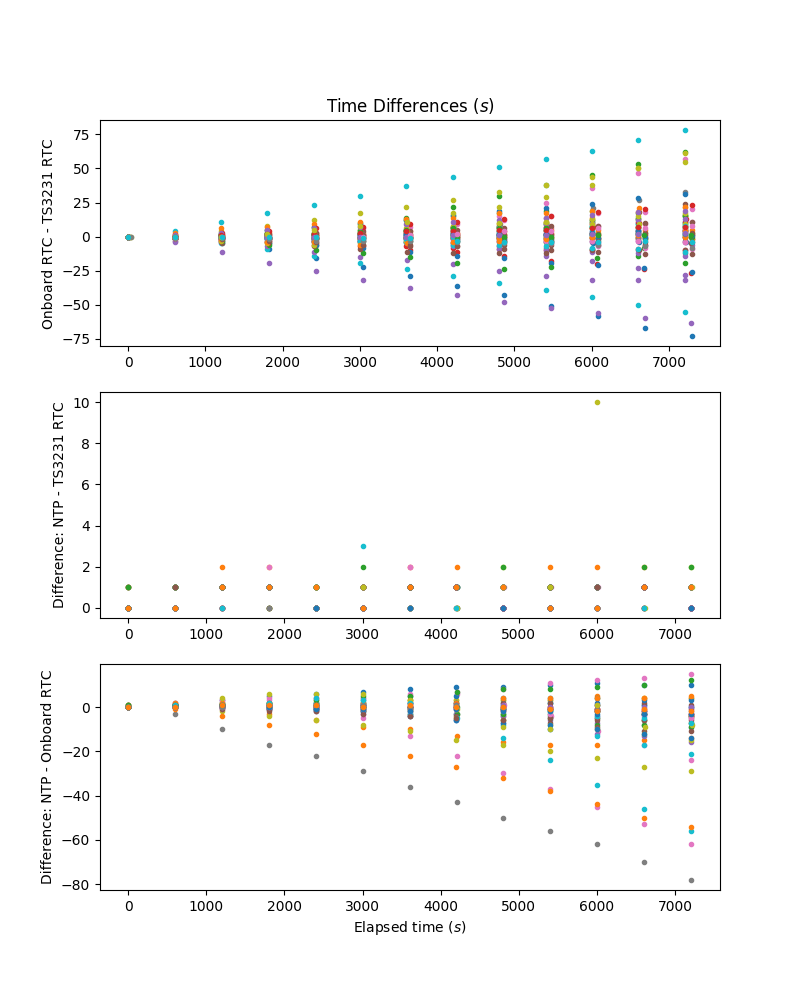
\includegraphics[width=\MFW]{Images/TimeAccPrecPlt1.png}}{https://publicsensors.org/IntroSensors/Images/TimeAccPrecPlt1.png}
			\caption[Plots of time-keeping errors]{Plots of time-keeping errors, indicated by differences among three methods of keeping time. 
			Top: Onboard \rtc minus \DS3231 \rtc. Middle: \ntp minus \DS3231 \rtc. Bottom: \ntp minus onboard \rtc. }
			\labfig{TAPplt1}
		\end{center}
	\end{marginfigure}
	
	When the scripts have run successfully, they will produce a set of plots like \reffig{TAPplt1}.
	\begin{itemize}
		\item[$\circ$] This example assumes the \lstinline{TimeData} subdirectory is in the same directory that contains \htmladdnormallink{TimeAccPrec.py}{https://publicsensors.org/IntroSensors/Codes/TimeAccPrec.py} and from which you launched the \python session.
		If you have used file names or directories other than these defaults, adjust your commands accordingly. 
		\item[$\circ$] The \lstinline{plt_style} parameter determines the type of symbol and line in the plots. 
		The value in the example, \lstinline{plt_style}, means that each data point will be plotted as a small circle, with no lines connecting sequential data points.
	\end{itemize}

	\item \textbf{Experiment with} \lstinline{matplotlib}\textbf{'s} \htmladdnormallink{interactive navigation widgets}{https://matplotlib.org/users/navigation_toolbar.html}:
	\begin{itemize}
		\item[$\circ$] The small buttons at the bottom left of the graphics window enable you to zoom and pan to different parts of your plots, and to save your figure as a \lstinline{png} or \lstinline{jpg} image.
		These images can be imported into a report or web page. 
		See the link above for detailed explanations of how these widgets work.  
		
		\smallskip
		When you are finished, close the figure window to be ready for the next steps in plotting data.
	\end{itemize}
%	\todo{milestone}
\loadMilestone{mlst:03a} % load milestone with tags id: mlst:02a

	\item \textbf{Replot time-keeping errors, using plotting symbols and line type to distinguish data from your own microcontroller/\rtc combination}:

	Repeat the commands you used to produce the previous plots, but instead of the previous call to \lstinline{lineplot_TC_data} substitute
\begin{lstlisting}[language=Python]
lineplot_TC_data(fig,axes,data_directory='TimeData',
        template="*.txt",plt_style='.',exclude='3648523')
lineplot_TC_data(fig,axes,data_directory='TimeData', 
        template="*3648523*.txt",plt_style='^:')
\end{lstlisting}
	where, as before, adjust as necessary to reflect your filenames and directories.
	\begin{marginfigure}[-19.cm]
		\begin{center}
			\htmladdnormallink{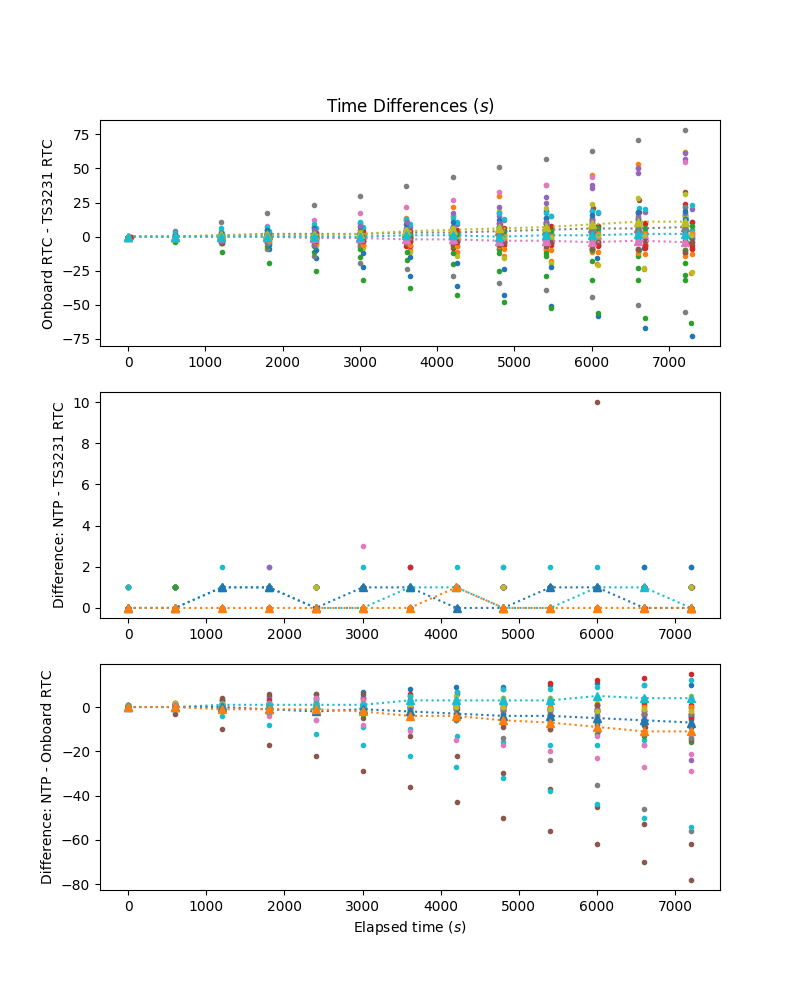
\includegraphics[width=\MFW]{Images/TimeAccPrecPlt2.png}}{https://publicsensors.org/IntroSensors/Images/TimeAccPrecPlt2.png}
			\caption[Plots of time-keeping errors]{Plots of time-keeping errors, indicated by differences among three methods of keeping time. 
			Triangles and dotted lines represent data from the focal microcontroller/\rtc combination. 
			Top: Onboard \rtc minus \DS3231 \rtc. Middle: \ntp minus \DS3231 \rtc. Bottom: \ntp minus onboard \rtc. }
			\labfig{TAPplt2}
		\end{center}
	\end{marginfigure}
	The resulting plot should look something like \reffig{TAPplt2}.
	\begin{itemize}
		\item[$\circ$] In the first of these commands, the parameter \lstinline{exclude='3648523'} means that any filename containing '3648523' will \underline{not} be plotted. 
		
		\smallskip
		'3648523' is the unique ROM ID of one of the microcontrollers used to collect the data archive. 
		Therefore, this command will plot all data 
		
		\item[$\circ$] In the second command, the parameter \lstinline{template="*3648523*.txt"} means that \underline{only} filenames containing '3648523' (and ending in `.txt') will be plotted. 
		
		\item[$\circ$] The parameter \lstinline{plt_style='^:'} means that data from filenames containing '3648523' will appear as triangles, connected by dotted lines.
		
		\item[$\circ$] Together, these commands results in plots showing data from microcontroller '3648523' as triangles connected by dotted lines, while all other data are plotted as unconnected circles.
		
		\smallskip
		Substitute your microcontroller's ROM ID into these commands to see how your microcontroller/\rtc combination compares to the overall population of 
		rtcs.
	\end{itemize}
%	\todo{milestone}
\loadMilestone{mlst:03b} % load milestone with tags id: mlst:02
	
	\item \textbf{Use the \python method \lstinline{subsample_TC_data} to collect a subsample of the time-keeping error data}:
	
	Use a command like:
\begin{lstlisting}[language=Python]
(subsample_times,subsample_onbrd_ext,subsample_NTP_ext,subsample_NTP_onbrd)= \
subsample_TC_data(data_directory='TimeData', template="*.txt",sub_samples=[0,3,6,9,12],exclude='3648523')
\end{lstlisting}
	where as before you have adjusted the filenames and directory as necessary.

	In this command, the parameter \lstinline{sub_samples=[0,3,6,9,12]} means data will be retained only from sample numbers 0,3,6,9,and 12 (in this case, at half hour intervals because samples are ten minutes apart). 

	The ``subsample'' lists on the left side contain the elapsed time and error data from the selected sample numbers.
	
	\item \textbf{Replot the time-keeping plots, adding percentiles to inform you how your microcontroller/\rtc combination compares to the population of \rtcs}:
	To make this plot, repeating all the previous steps you used to create a figure window, parse and plot data, \etc, but before you ``show'' the plot execute the command
\begin{lstlisting}[language=Python]
prcntplot_TC_data(fig,axes,subsample_times,subsample_onbrd_ext,
      subsample_NTP_ext,subsample_NTP_onbrd,pcnts=[5.,25.,50.,75.,95.])
\end{lstlisting}
	This command uses the subsampled data to generate plots with lines for specified percentiles.
	In this case, the parameter \lstinline{pcnts=[5.,25.,50.,75.,95.]} specifies that the 5th, 25th, 50th, 75th and 95th percentiles are to be plotted.
	\begin{marginfigure}[-19.cm]
	\begin{center}
		\htmladdnormallink{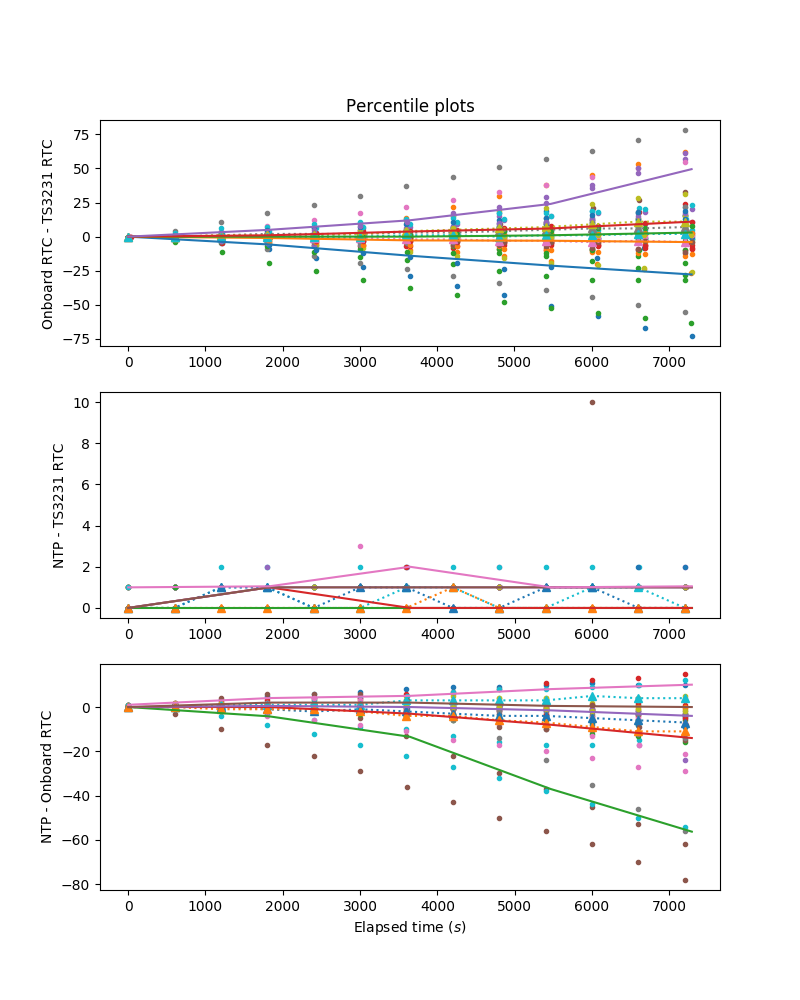
\includegraphics[width=\MFW]{Images/TimeAccPrecPlt3.png}}{https://publicsensors.org/IntroSensors/Images/TimeAccPrecPlt3.png}
		\caption[Plots of time-keeping errors]{Plots of time-keeping errors, indicated by differences among three methods of keeping time. 
		Triangles and dotted lines represent data from the focal microcontroller/\rtc combination. 
		Solid lines represent selected percentiles (5th, 25th, 50th, 75th and 95th), excluding data from the focal microcontroller/\rtc combination. 
		Top: Onboard \rtc minus \DS3231 \rtc. Middle: \ntp minus \DS3231 \rtc. Bottom: \ntp minus onboard \rtc. }
		\labfig{TAPplt3}
	\end{center}
\end{marginfigure}

	\smallskip
	The resulting plot --- something like \reffig{TAPplt3} --- enables you to see at a glance how the time-keeping errors from your microcontroller/\rtc combination compare to various percentiles of errors from the population of devices.
%	\todo{milestone}
\loadMilestone{mlst:03c} % load milestone with tags id: mlst:02
	
	\item \textbf{Generate violin plots to visualize the distributions of time-keeping errors in the subsampled data}:
\begin{lstlisting}[language=Python]
violinplot_TC_data(fig,axes,subsample_times,subsample_onbrd_ext,subsample_NTP_ext,subsample_NTP_onbrd,v_widths=200.,bw=0.5)
\end{lstlisting}
	\begin{marginfigure}[0.cm]
	\begin{center}
		\htmladdnormallink{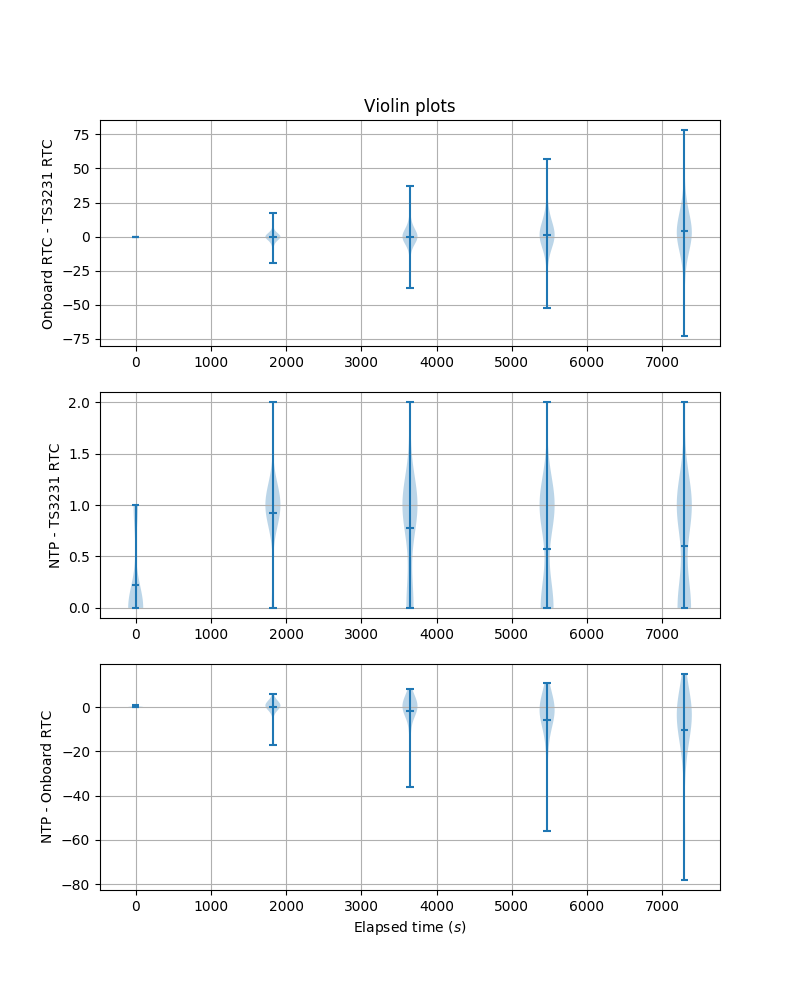
\includegraphics[width=\MFW]{Images/TimeAccPrecPlt4.png}}{https://publicsensors.org/IntroSensors/Images/TimeAccPrecPlt4.png}
		\caption[Violin plots of time-keeping errors]{Violin plots of time-keeping errors, indicated by differences among three methods of keeping time.
		Top: Onboard \rtc minus \DS3231 \rtc. Middle: \ntp minus \DS3231 \rtc. Bottom: \ntp minus onboard \rtc. }
		\labfig{TAPplt4}
	\end{center}
\end{marginfigure}
	This command results in plots like \reffig{TAPplt4}.
	You can vary the parameters \lstinline{v_widths=200.,bw=0.5} to adjust the width and breadth of the resulting distributions to get a good representation of your data.
	Details about implementation of violin plots are given in \lstinline{matplotlib}'s \htmladdnormallink{documentation}{	https://matplotlib.org/3.1.1/api/_as_gen/matplotlib.pyplot.violinplot.html}.
	
	Note the differences in vertical axes. 
	What can you say about the distributions of time-keeping errors?
	Are they \texttt{unimodal} or \texttt{multi-modal}?
	Do they reflect directional biases towards being more often negative than positive, or \textit{vice versa}?
	What can you say, based on the plots you've generated, about the relative magnitudes of errors for the different time-keeping methods?
%	\todo{milestone}
\loadMilestone{mlst:03d} % load milestone with tags id: mlst:02
	
\end{enumerate}

\subsection{Hypothesis tests about \rtc accuracy and precision}
We now turn to \emph{hypothesis tests} about errors associated with the different methods of keeping time with microcontrollers. 
Recall that hypothesis tests quantify the probability an observed outcome occurred by chance, if some assumptions about the statistical distributions are true.
The tests are usually posed in the form of a \emph{null hypothesis}, e.g. that two datasets are drawn from the same distribution. 

Statistical analysis enables us to calculate the probability with which the observed results could have happened, assuming the assumptions and null hypothesis are true. 
The lower the resulting probability, the less likely it is that the null hypothesis is true.
If the probability is less than a threshold --- usually $0.05$, or 1 in 20 --- we consider it so unlikely that we accept the null hypothesis is \emph{falsified}.
Falsifying the hypothesis that two distributions are the same implies that the distributions are significantly different.

Note that the converse does not apply. 
If the resulting probability is above the threshold, that does not prove the distributions are the same --- only that we failed to establish that they are different.
It may be that they are truly the same, but it may also be that they are different and our statistical sampling was insufficient to demonstrate it.

For example, consider the question ``Is my \rtc defective?'' 
In statistical terms, this question can be made more explicit by restating it as ``Are the time-keeping errors from my \rtc different than the errors from the whole population of \rtcs?''
This statistical form of the question can be tested in the form of a null hypothesis: 
\begin{itemize}
	\item[$\circ$]The distribution of errors from my \rtc is the same as the distribution of errors from the  whole population of \rtcs.
\end{itemize}
Because you have time-keeping error samples from your \rtc and a population of other \rtcs, you can estimate the probability that your samples could have been drawn from the whole population of \rtcs.
This probability can be estimated in several ways, depending on what we know about the characteristics of the distributions. 

If we know nothing about the observed error distributions, or if we know their shapes but they does not conform to any standard distribution, we can use \emph{non-parametric tests}.
Non-parametric tests rely only on the order of samples in two datasets, not the shape of their distributions.
Among the most useful non-parametric tests are:
\begin{itemize}
	\item[$\circ$] The \emph{Wilcoxon rank-sum test}, which tests the \htmladdnormallink{null hypothesis that two sets of samples are drawn from the same distribution}{https://docs.scipy.org/doc/scipy/reference/generated/scipy.stats.ranksums.html\#scipy.stats.ranksums}. 
	\item[$\circ$] The \emph{Kruskal-Wallis H-test}, which tests the  \htmladdnormallink{null hypothesis that the medians of two datasets are the same}{https://docs.scipy.org/doc/scipy/reference/generated/scipy.stats.kruskal.html\#scipy.stats.kruskal}.
\end{itemize}
Applied to your datasets, if either or both of these null hypotheses can be falsified, the implication is that your \rtc is defective.
If neither can be falsified, that implies a lack of evidence that your \rtc is defective. 
That is, the combination of the data and non-parametric tests lack the \emph{power} to establish a significant difference.
The possibility remains that with much larger sample size, or longer sampling time, the hypotheses could be falsified. 
Or, your \rtc might really not be defective!

If we knew that time-keeping errors conform to a standard distribution, we might be able to use more discriminating hypothesis tests.
For example, if we knew that these errors are normally distributed, we could use
\begin{itemize}
	\item[$\circ$] The \emph{T-test}, which tests the  \htmladdnormallink{null hypothesis that the means of two sets of normally distributed data are the same}{https://docs.scipy.org/doc/scipy/reference/generated/scipy.stats.ttest_ind.html\#scipy.stats.ttest_ind}.
\end{itemize}
The \emph{T-test} null hypothesis is similar to the \emph{Kruskal-Wallis H-test}, but focuses on the mean rather than the median.
The requirement that both datasets have normal (a.k.a. \emph{Gaussian}) distributions means that the plausible range of means can be better constrained.
Compared to the non-parametric tests, this tighter constraint makes the \emph{T-test} more powerful for a given set of data. 
A \emph{T-test} can potentially falsify the null hypothesis even when the corresponding \emph{Kruskal-Wallis H-test} can not.

\subsubsection{\howto Probability plots and hypothesis tests with \rtc data}
\begin{enumerate}
	\item \textbf{If they are not already imported, import the required \python libraries}:
\begin{lstlisting}[language=Python]
import matplotlib.pyplot as plt
import scipy.stats as stats
from TimeAccPrec import * 
\end{lstlisting}
	\item \textbf{Separately sub-sample the data from your \rtc and from all the other \rtcs, with a modification of}:
\begin{lstlisting}[language=Python]
(subsample_times,subsample_onbrd_ext,subsample_NTP_ext,subsample_NTP_onbrd)= \
     subsample_TC_data(data_directory='TimeData', template="*.txt",sub_samples=[0,3,6,9,12],exclude='3648523')
(subsample_times2,subsample_onbrd_ext2,subsample_NTP_ext2,subsample_NTP_onbrd2)= \
     subsample_TC_data(data_directory='TimeData', template="*3648523*.txt",sub_samples=[0,3,6,9,12])
\end{lstlisting}
	\item \textbf{Graphically assess whether the error distributions conform to a normal distribution}:
\begin{lstlisting}[language=Python]
fig,axes=plt.subplots(nrows=3,ncols=1,figsize=(8,10))
dstr=stats.norm
probplot_TC_data(axes[0],subsample_onbrd_ext,'onbrd_ext',dst=dstr)
probplot_TC_data(axes[1],subsample_NTP_ext,'NTP_ext',dst=dstr)
probplot_TC_data(axes[2],subsample_NTP_onbrd,'NTP_onbrd',dst=dstr)
# Add a title and "show" the plots:
axes[0].set_title('Probability plots')
plt.show()
\end{lstlisting}
	\begin{marginfigure}[-19.cm]
	\begin{center}
		\htmladdnormallink{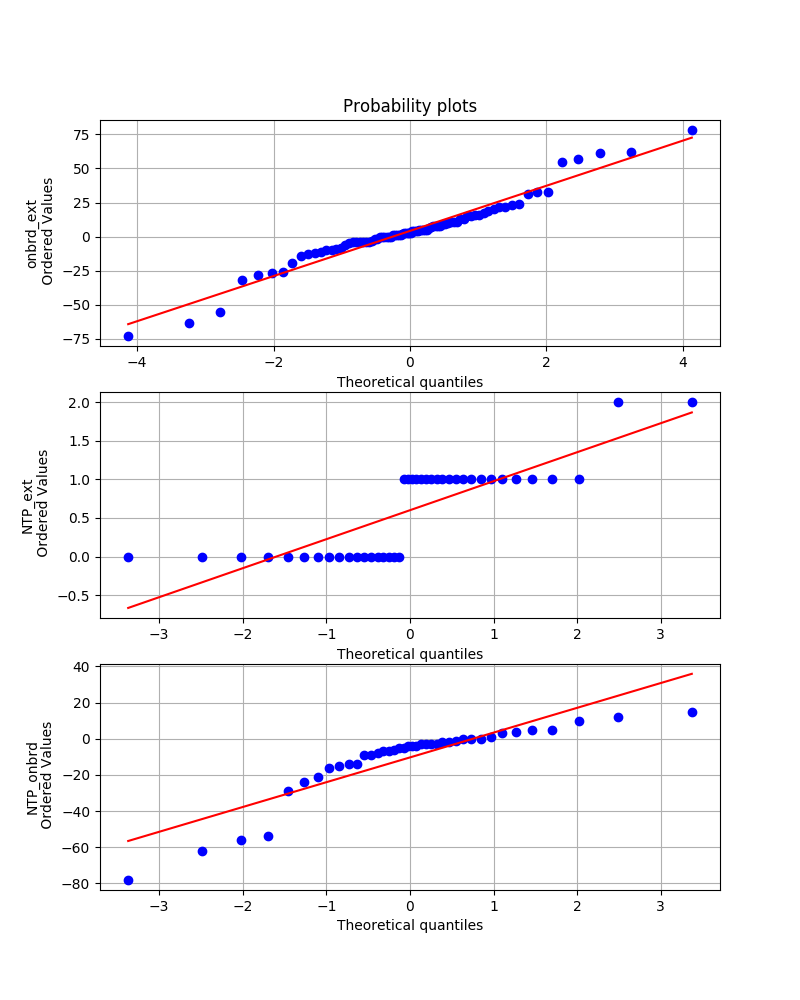
\includegraphics[width=\MFW]{Images/TimeAccPrecPlt5.png}}{https://publicsensors.org/IntroSensors/Images/TimeAccPrecPlt5.png}
		\caption[Probability plots of time-keeping errors]{Probability plots of time-keeping errors assuming a normal distribution, indicated by differences among three methods of keeping time.
			Top: Onboard \rtc minus \DS3231 \rtc. Middle: \ntp minus \DS3231 \rtc. Bottom: \ntp minus onboard \rtc. }
		\labfig{TAPplt5}
	\end{center}
\end{marginfigure}
	The result of these commands, similar to \reffig{TAPplt5}, indicate which differences among time-keeping methods conform to a normal distribution.
	The closer the plotted data points lie to the red line, the more normally distributed they are.
	
	\smallskip
	Note that \lstinline{probplot_TC_data} plots only the last sampling interval in the subsampled dataset. 
	
	\smallskip
	\texttt{scipy}'s plotting algorithm also provides some useful quantitative metrics:
	\begin{itemize}
		\item[$\circ$] The \texttt{intercept} of the regression (red) line indicates the mean of the approximating normal distribution.
		\item[$\circ$] The \texttt{slope} of the regression (red) line indicates the variance of the approximating normal distribution.
		\item[$\circ$] The square root of the \texttt{Coefficient of Determination} indicates goodness of fit between the data and the approximating normal distribution.
	\end{itemize}
	
	
	In \reffig{TAPplt5}, the differences in the archived dataset between the onboard and external \rtcs (top plot) are reasonably close to normally distributed.
	There are noticeable deviations at the left and right sides (corresponding to the tails of the distributions). 
	The other error distributions appear less consistent with a normal distribution.
\loadMilestone{mlst:03e} % load milestone with tags id: mlst:02

	\item \textbf{Perform hypothesis tests comparing your \rtc to the whole population of \rtcs}:
\begin{lstlisting}[language=Python]
hypothesis_TC_data(subsample_times,subsample_onbrd_ext,subsample_onbrd_ext2,pcnts=[5.,25.,50.,75.,95.])
\end{lstlisting}
	In this example, we have focused on the time-keeping differences between the onboard and external \rtcs,but in working with your data you can make other comparisons.

	\smallskip
	The output of this command has two parts:
	\begin{itemize}
		\item[$\circ$] The first part of the output summarizes the distributions by printing out their percentiles at each of the sub-sampling intervals.
		\item[$\circ$] The second part prints out the results of three hypothesis tests (Kruskal-Wallis H-test, Wilcoxon rank-sum and T-test) at each of the sub-sampling intervals.
		
		\smallskip
		The key output is the $p$-value, representing the probability of getting the observed data if the null hypothesis is true.
		
		\smallskip
		Note that the T-test analysis gives a result, but that result has statistical validity only if the underlying assumption that time-keeping errors are normally distributed are satisfied.
	\end{itemize}

\end{enumerate}
\loadMilestone{mlst:03f} % load milestone with tags id: mlst:02


\subsection{Environmental effects on \rtc accuracy and precision}
At this point, you have developed the skills to build a dataset of time-keeping errors, using differences among the three methods of time-keeping. 
You have experience in a variety of plotting techniques, that enable you to visualize the overall distribution of time-keeping errors, the percentiles of devices that show specific magnitudes and directions of errors, and how a sub-sample of devices compare to the entire population. 
You have also applied hypothesis testing techniques, with consideration of which statistical tests are applicable to the error distributions in your dataset.
This work has given you a basis for anticipating which time-keeping methods are most accurate and precise, how large errors are likely to be, and whether a given device appears to be more error-prone than expected.

It's worth considering how these results apply to the sensors you will deploy in the field. 
Field conditions for environmental sensors vary widely, including wide ranges in temperature, humidity, salinity, incident solar radiation, pressure, and other environmental parameters. 
Because your microcontroller/\rtc combination will be within an environmental housing, it will not be exposed to many of these variations. 
However, environmental housings do not typically insulate devices from temperature fluctuations.
In fact, the internal temperatures inside housings often range over much wider extremes than the ambient environment.
For example, temperature inside an environmental housing exposed to direct sunshine can reach 10s of degrees higher than the surrounding air. 
Conversely, internal temperature can reach well below freezing.

Temperature has strong effects on many electrical and mechanical material properties. 
For this reason, devices with \rtcs have built-in thermometers, and algorithms to compensate for temperature effects on vibrating crystals and other components.
There is clearly the possibility that these thermometers and algorithms involve substantial additional errors.
If so, the performance of our time-keeping devices might be very different in the field than in our laboratory tests.

In generating and analyzing the time-keeping datasets, we have not paid particular attention to environmental conditions. 
During data collection, the microcontrollers and \rtcs were likely under relatively comparable conditions, e.g. in the same laboratory, or under similar but haphazardly varying conditions (e.g. room temperatures in different classmates' houses).
By repeating your data collection and analysis, but with an experimental design that explicitly designates two subpopulations operating at different temperatures, you can quantify the effects (if any) of temperature on the error distributions of time-keeping devices.

\subsubsection{\howto Quantifying temperature effects on time-keeping errors}
Use the methods of this chapter in collaboration with your classmates to test the null hypothesis that:
\begin{itemize}
	\item[$\circ$] Time-keeping errors from microcontroller/\rtc combinations operated at environmentally relevant low and high temperatures have the same statistical distributions.
\end{itemize}
\begin{enumerate}
	\item \textbf{Agree on a consensus sampling protocol, with subpopulations divided into ``hot'' and ``cold'' subpopulations.}
	
	In designing your protocol, consider the trade-offs between longer sample duration \textit{vs} more replicates, within a practical total available time for data collection.
	In choosing ``hot'' and ``cold'' temperatures for this experiment, it's likely that you will need to make concessions to practical constraints.
	In many cases, using outdoor conditions for the hot or cold subpopulations might be practical.
	Make sure, however, that your devices are protected from moisture and other damaging conditions, e.g. by placing them in a sealed plastic bag. 
	
	\item \textbf{Visualize the resulting populations, using different plotting symbols and line types to indicate how percentiles evolve over time and assess distribution shapes.}
	\item \textbf{Perform statistical tests of the null hypothesis, using the non-parametric tests and --- if justified --- the \texttt{T-test}.}
	
	
\end{enumerate}

\loadMilestone{mlst:03g} % load milestone with tags id: mlst:02


%This provides a basis for 
%
%DEFINE HYPOTHESES TO START WITH:
%-- ONE RTC IS DIFFERENT FROM OTHERS
%-- ERRORS DUE TO METHOD X ARE WITHIN BOUNDS Y
%-- ERRORS ARE A FUNCTION OF ENVIRONMENT E.G. TEMPERATURE
%
%will assess the relative \emph{accuracy} and \emph{precision} of each method. 
%Refer to the \refsec{acc_prec} if you want a reminder of the distinctions between accuracy and precision.
%



%of observed timekeeping errors (). 
%(A) Data parsing and visualization (1.5 points) 
%In this section of the problem set, you will use a python script to parse and plot our dataset. The script is called \lstinline{analyze_acc_prec_OCN351.py}, and it is posted in Files>MicroPython on Canvas. 
%
%Download \lstinline{analyze_acc_prec_OCN351.py}, and place it in your python code folder.
%
%The dataset is also posted in the MicroPython directory, in a zipped archive called PS1timedates.zip. Download and unzip this file into a directory on your computer.
%
%Modify the code to make it work on your machine. This step may take some trial and error – please contact the instructors if you have persistent trouble with any of the necessary adjustments.
%
%One change you will need to make is to edit the string \lstinline{data_directory} (line 14), so that it points to the folder in which you placed the PS1timedates data directory. Keep in mind that, in Linux OS, the separator between different levels in the file structure is a ``/''. It is the same on MacOS, but different on Windows. 
%
%When this python code executes, it reports the names of the data files it has found and the number of lines it parsed from each. This makes it easy to tell whether the directory information is correct.
%
%When execution is complete, you should see a graphics window with 6 plots. In each row, the left column is a plot of the observed differences between two time sources. The right plot is a violin plot, in which the blue shading represents an estimate of the distribution of differences at specific time points (determined by sample numbers in violin\textunderscore sample). Error levels where the shading is wide are relatively more frequent in the data than levels where the shading is narrow.
%
%
% After making adjustments so that your code finds the data and produces plots, spend a few minutes experimenting with settings and parameters to see what they do. 
%
%The width and degree of smoothing in the violin plots are determined by the parameters v\textunderscore widths and bw. Do some settings appear more informative about timekeeping errors than the default ones?
%
%Save the figure(s) you produce by clicking the rightmost icon on the bottom bar.



	
%How can we quantify time-keeping errors? 
%
%To begin with, we need some way to determine ``true'' time, from a reference time source that we believe to have time-keeping errors that are so small as to be negligible for our purposes. 
%An example is the \htmladdnormallink{official time source}{https://www.time.gov/} for the U.S. government, operated by the National Institute of Standards and Technology (NIST).
%
%Assuming we have an accurate reference, let's suppose we use a device to take a large number --- hundreds or even thousands --- of time measurements, over a specific ``true'' time interval, such as an hour. 
%
%How do we know what ``true'' time? We need to use a reference time source, 


%We will collect timestamp data from each of your microcontrollers to answer the following questions:
%\begin{itemize}
%	\item How accurate and precise are each of the methods of obtaining the current time?
%	\item Do the RTCs on different microcontrollers differ \emph{systematically} from each other (that is, are particular \rtcs biased towards run fast or slow)?
%	\item Does the magnitude and direction of timekeeping error depend on environmental conditions (e.g. temperature)?  
%\end{itemize}




\pagelayout{wide} % No margins
\addpart{Working with environmental sensors}
%\addpart{Working with electrical circuits}
\pagelayout{margin} % Restore margins

\setchapterstyle{kao}
\setchapterpreamble[u]{\margintoc}
\chapter[Environmental sensing with voltage, current and resistance]{Introduction to circuits: Environmental sensing with voltage, current and resistance}
\labch{circuits_intro}
Natural environments and the ecosystems within them are governed by physical characteristics like temperature, light intensity, $O_2$ concentration, $pH$, seawater salinity, and wind or current velocity.
Instruments for environmental sensing generate electrical signals that vary with one or more of these characteristics.
For this to be useful, the relationship between electrical outputs and environmental inputs must be consistent and quantifiable. 
The process of establishing this quantitative relationship is called \emph{calibration}.
A calibration usually must work in both directions:
First, the calibration is established by measuring the electrical signals across a relevant range of known environmental conditions.
Then,  electrical signals are acquired from unknown environmental samples, and the calibration is used to infer the conditions under which they were obtained.
This chapter will guide you through the methods and process of designing and building devices to measure electrical signals, and calibrating those devices to quantify environmental conditions.

Because most environmental characteristics vary continuously, the electrical signals generated by environmental sensors are also usually continuous. 
These signals are referred to as \emph{analog} signals, to distinguish them from \emph{digital} signals like those you worked with in \refch{first_exercises}. 
Digital signals are simply ``high'' or ``low'' --- usually determined by a voltage that is above or below a threshold voltage.
Because analog signals vary continuously, they potentially carry much more information.
However, analog signals must typically be measured much more accurately and precisely than digital signals. 
For this reason, analog measurements are handled differently by microcontrollers, with distinct methods and constraints. 
 
Most microcontrollers can directly measure just two parameters: voltage and time. 
Unsurprisingly, the vast majority of analog sensors provide information using one or both of these parameters. 
A voltage-based analog sensor typically has three connections: ground, \texttt{GND} (\texttt{0V}); an input voltage, $V_{in}$; and, a data output voltage, $V_{data}$.
The data output voltage, $V_{data}$, represents environmental characteristics in the form of a voltage that varies between \texttt{GND} and $V_{in}$.
For example, in \refsec{cal_therm}, you will measure temperature with a component called a thermistor. 
A thermistor has a \emph{resistance} (impediment to the flow of electrons) that changes as a function of temperature.
You will combine the thermistor with another resistor in a way that causes the output voltage $V_{data}$ to change with temperature. 
You will then use a microcontroller to measure $V_{data}$, calculate thermistor resistance, and use a calibration to infer the temperature.

A time-based sensor uses the duration of or interval between events as the key measurement.
For example, in \refsec{cal_sonar}, you will use an acoustic sensor to measure distance to a object.
In this case, the length of time between an initial event --- sending out a pulse of sound --- and a secondary event --- the echo of that pulse arriving back at the source --- indicates the round trip travel time for sound waves.
Calibrated by a knowledge of the speed of sound, this travel time indicates distance.

The following sections explain some electrical principles that you need to understand when working with voltage-based environmental sensors. You will apply that knowledge to measure battery voltage (an important parameter in a field-deployed device!) and thermistor temperature. You will then use time-based sensors to measure distance and light, and combine both time and voltage to measure wind or current velocity. 
\todo{Textbox explaining font conventions for code, units and electrical quantities.}

%like the \texttt{3V3} pin in your \refch{first_exercises} circuits), 
%The data connection takes on a voltage anywhere between 
%
%have a is the process of generating 
%
%calibration must be bidirectional
%
%In this chapter, we explore the relationships between characteristics of the environment --- \etc ---

\section{Measuring voltage}
\labsec{meas_volt}
Voltage is measured on a microcontroller using an \texttt{Analog to Digital Conversion} (\adc) pin.
\adc pins act as inputs, just as digital \texttt{GPIO} pins do in their input modes.
However, reading the value of a digital \texttt{GPIO} pin results in either 1 or 0 (``high'' or ``low''). In contrast, an \adc pin returns an integer that can span a range, e.g. between 0 and 1024.
That integer's value is proportional to the voltage applied to the \adc pin. 

For example, in \htmladdnormallink{\texttt{Analog to Digital Conversion} on the ESP8366}{http://docs.micropython.org/en/v1.9.3/esp8266/esp8266/quickref.html\#adc-analog-to-digital-conversion}, an \adc value of 0 implies \texttt{0V}, \adc value of 1024 implies \texttt{1V}, and \adc value of 113 implies $\frac{113}{1024} \times 1\mathtt{V}$ or \texttt{0.11V}. 
In general,
\begin{equation}\label{adc_volt}
V = \frac{ADC}{1024} 
%V \mathsf{V} \mathrm{V} = \frac{ADC}{1024} \frac{\mathsf{ADC}}{1024} \frac{\mathrm{ADC}}{1024} 
\end{equation}
for the \texttt{ESP8266}, where $ADC$ is the integer value read from the \adc pin, and $V$ is the applied voltage in units of \texttt{volts}
\sidenote[][*-8]{
	\begin{kaobox}[backgroundcolor=\SNcolor,frametitlebackgroundcolor=\SNcolor,frametitle=Resolve to change!]
		An important implication of Equation \ref{adc_volt} is a limit to the \htmladdnormallink{\emph{resolution}}{https://www.itl.nist.gov/div898/handbook/mpc/section4/mpc451.htm} of the \texttt{ESP8266}'s \adc.
		Resolution is the smallest increment of a physical characteristic that can be distinguished by a sensor. 
		In this case, an increment of 1 in the integer value of the \texttt{ESP8266}'s \adc corresponds to a change of voltage, $\Delta V$, of 
		\begin{equation}\label{adc_volt2}
		\Delta V = \frac{1~ \mathtt{volts}}{1024} = 0.000977~ \mathtt{volts}
		\end{equation}
		This means that, even if there were no measurement errors associated with accuracy and precision, the \adc reading could represent any voltage within a range of approximately $\pm \frac{1}{2}\Delta V$. 
	\end{kaobox}
}.

\subsection{Voltage of an \texttt{18650} lithium-ion battery}
The task at hand in this section is to measure the voltage of a rechargeable lithium-ion battery called an \htmladdnormallink{``\texttt{18650}''}{https://en.wikipedia.org/wiki/Lithium-ion_battery}.
The name \texttt{18650} derives from its dimensions: an \texttt{18650} battery is \texttt{18mm} in diameter and \texttt{65mm} long.
\texttt{18650}s are a common standard of rechargeable battery, widely available and well suited to powering environmental sensors. 

\texttt{18650} voltages typically range from 3.7-4.2V, depending on how charged they are, ambient temperature, \etc
For an instrument in the field, the capacity to monitor its own battery level can be valuable.
For example, an instrument on the verge of power failure can, if connected to the Internet, send a message indicating it needs maintenance.
Alternatively, it can be programmed to alter its sampling schedule to stretch whatever power remains over a longer duration, even if less frequently.

Monitoring battery voltage with an \adc that measures voltage seems like an easy task, right?

Well, it \emph{is} pretty easy.
But, there's a wrinkle we need to contend with: \adcs have strict limits to how large a voltage they can tolerate.
In fact, for many types of microcontroller these limits are quite low.
For \texttt{ESP8266}s, the limit is \texttt{1V}.
That's much lower than even a mostly discharged \texttt{18650} battery's voltage.
If we attach the terminals of an \texttt{18650} directly to an ESP8266 \adc, we risk destroying the \adc and possibly other components as well.

We need a way to \emph{represent} the voltage of an \texttt{18650} with a voltage that we know will never exceed \texttt{1V}.
To accomplish this, we'll create a sensor in the typical 3-connection analog format: \texttt{GND}, $V_{in}$ and $V_{data}$.
In this sensor, \texttt{GND} and $V_{in}$ will come from the \texttt{18650} terminals. 
$V_{data}$ will come from the circuit we're about to design, in such a way as to insure that it accurately represents battery voltage according to a known calibration while staying within the \texttt{1V} limit.

\subsubsection{Ohm's Law for voltage, current and resistance}
The design of our current sensor is based on one of the fundamental laws governing electricity, \htmladdnormallink{Ohm's Law}{https://en.wikipedia.org/wiki/Ohm\%27s\_law}.
Ohm's Law defines the quantitative relationship between voltage, current and resistance across a \htmladdnormallink{\emph{resistor}}{https://en.wikipedia.org/wiki/Resistor}.
You used a resistor when you constructed a circuit to power an external LED in \refsec{ext_led}.
Though we did not go into the details there, the purpose of that resistor was to regulate the amount of current flowing through the LED. 
How did we know which resistor to use?
We calculated it using Ohm's Law.

In a diagram of an electrical circuit, a resistor is illustrated by a zig-zag line:
\begin{figure}[H]
	\begin{center}
		\begin{tikzpicture}[american voltages]
		\draw
		(0,0) to [short,l=$V_{1}$, *-] (1,0)
		to [R, l=$R$, i_=$I$] (3,0)
		to [short,l=$V_{2}$, -*] (4,0);
		\end{tikzpicture}
		\caption[Circuit diagram: Resistor]{Circuit diagram of a resistor.}
		\labfig{res}
	\end{center}
\end{figure}

In this circuit, $R$ is the value of the resistor.
The voltage drop across this resistor is $V = V_1 - V_2$.
The current flowing through the resistor is $I$.

According to Ohm's Law,
\begin{equation}\label{OhmsVIR}
V = I R
\end{equation}
In Equation \ref{OhmsVIR}, $V$ is the voltage difference measured across the resistor, in units of \htmladdnormallink{\texttt{volts}}{https://en.wikipedia.org/wiki/Volt}.
$I$ is the current (i.e., the flow of electrons) through the resistor, in units of \htmladdnormallink{\texttt{amperes}}{https://en.wikipedia.org/wiki/Ampere} (usually shortened to ``\texttt{amps}'').
$R$ is the \emph{resistance} of the conductor, in units of \htmladdnormallink{\texttt{ohms}}{https://en.wikipedia.org/wiki/Ampere}.


\begin{kaobox}[frametitle=Signs of things to come \dots]
Current consists of flowing electrons.
This means that whenever we refer to a value like $I$ to indicate current, we need to be clear about which direction of flow we count as positive.
This will become especially important when we work with more complex circuits later on.

In the circuit diagram, the small arrow above $I$ indicates the direction we choose to count current flow as positive.
We can choose either direction, but we must be consistent in using one direction or the other. 
For that reason, the direction of positive current flow will always be indicated in the circuit diagrams in this book.

%Because no electrons are created or lost while passing through the resistor, the current is the same at every point in this simple circuit.

The arrow also tells us the direction in which to measure voltage drop: 
The arrow always points away from the starting voltage ($V_1$) and towards the ending voltage ($V_2$).
So, the voltage drop in the diagram is $V=V_1-V_2$.

Current always flows from a higher voltage to a lower voltage.
That is, if $V>0$, current flows from left to right and $I$ takes on a positive value.
If $V<0$, current flows from right to left and $I$ takes on a negative value.
%We need only one variable for current, because the number of flowing electrons is not changed inside a resistor --- the current flowing in from the left side is the same as the current flowing out of the right side.
\end{kaobox}

%https://en.wikipedia.org/wiki/Hydraulic_analogy

%Two mathematically equivalent forms of Ohm's Law are found by solving for $I$ or $R$:
%\begin{eqnarray}
%I = \frac{V}{R} \label{OhmsIVR} \\
%R = \frac{V}{I}  \label{OhmsRVI}
%\end{eqnarray}
Together, the three forms\sidenote[][*-8]{
	\begin{kaobox}[backgroundcolor=\SNcolor,frametitlebackgroundcolor=\SNcolor,frametitle=Ohm I!]Ohm's Law states that the current $I$ through a resistor $R$ due to the voltage difference $V$ is
		\begin{equation*}%\label{OhmsVIR}
			V = I R
		\end{equation*}
		Two mathematically equivalent forms of Ohm's Law are found by solving for $I$ or $R$:
		\begin{eqnarray}
		I = \frac{V}{R} \label{OhmsIVR} \\
		R = \frac{V}{I}  \label{OhmsRVI}
		\end{eqnarray}
		Together, the three forms of Ohm's Law make clear that among the three quantities $V$, $I$ and $R$, any two known values determine the third.	
	\end{kaobox}
} of Ohm's Law (Equations \ref{OhmsVIR}-\ref{OhmsRVI}) show us how to use two of the quantities $V$, $I$ and $R$ to determine the third.

For example:
\begin{itemize}
	\item  If we know that $I=0.5$ amps and $R=4$ ohms, Equation \ref{OhmsVIR} tells us that $V=0.5 \times 4 = 2$ volts.
	\item  If we know that $V=7$ amps and $R=2$ ohms, Equation \ref{OhmsIVR} tells us that $I= \frac{7}{2} = 3.5$ amps.
	\item  If we know that $V=12$ amps and $I=6$ ohms, Equation \ref{OhmsRVI} tells us that $R= \frac{12}{6} = 2$ ohms.
\end{itemize}

\subsubsection{Designing a \texttt{voltage divider} using Ohm's Law}
We'll now apply Ohm's Law several times to understand voltage, current and resistance in a configuration of two resistors called a \htmladdnormallink{\texttt{voltage divider}}{https://en.wikipedia.org/wiki/Voltage\_divider}.
A voltage divider is a simple circuit composed of two resistors, connected in \emph{series} so that a wire from one resistor is connected directly to one wire from the other.

%\begin{marginfigure}[-5cm]
\begin{figure}[H]
\begin{center}
	\begin{tikzpicture}[american voltages]
	\draw
	(0,0) to [short,l=$V_{in}$, *-] (1,0)
	to [R, l=$R_1$] (3,0)
	to [short, i_=$I$,l=$V_{data}$] (4,0)
	to [R, l=$R_2$] (6,0)
	to [short,l=GND, -*] (7,0);
%	(0,0) to [short, *-] (6,0)
%	to [V, l_=$\mathrm{j}{\omega}_m \underline{\psi}^s_R$] (6,2) 
%	to [R, l_=$R_R$] (6,4) 
%	to [short, i_=$\underline{i}^s_R$] (5,4) 
%	(0,0) to [open, v^>=$\underline{u}^s_s$] (0,4) 
%	to [short, *- ,i=$\underline{i}^s_s$] (1,4) 
%	to [R, l=$R_s$] (3,4)
%	to [L, l=$L_{\sigma}$] (5,4) 
%	to [short, i_=$\underline{i}^s_M$] (5,3) 
%	to [L, l_=$L_M$] (5,0); 
	\end{tikzpicture}
\caption[Voltage divider schematic]{Schematic diagram of a voltage divider circuit.}
\labfig{volt_div}\end{center}
\end{figure}
%\end{marginfigure}

\todo{Textbox contrasting series and parallel connections.}
A voltage divider has the same 3-connection configuration as most analog sensors.
The open ends of the resistor pair are connected to voltage inputs, $V_{in}$ on the left side and \texttt{GND} on the right.
%In our case, one is connected to \texttt{GND} (\texttt{0V}), and the other to $V_{in}$.
%\todo{Image of voltage divider}
These form two of the three connections in our analog voltage sensor.

In a diagram of a circuit, a junction between two components is often called a \emph{node}. 
The node between the two resistors is the third connection, the voltage output $V_{data}$.

What voltage does $V_{data}$ take on?

To calculate this voltage, we need to use the fact that any current flowing out of resistor $R_1$ must flow into the connected resistor, $R_2$.
That is, current is constant throughout the voltage divider circuit. 
%In this simple circuit geometry, there is no other conductive path for it to take!
%In the voltage divider circuit schematic, this means that $I_1=I_2$. 

With this constraint in mind, we can deduce the current flow through the circuit, the voltage $V_{data}$ at the middle node, and even the power the sensor uses while connected to \texttt{GND} and $V_{in}$.
The logic begins with applying Equation \ref{OhmsIVR} twice, once across each resistor:
\begin{itemize}
	\item Across resistor $R_1$, the voltage drop is $V_{in}-V_{data}$ \texttt{volts}.
	
	Therefore,
	\begin{equation}\label{vd1}
	I = \frac{V_{in}-V_{data}}{R_1}.
	\end{equation}	
	\item Across resistor $R_2$, the voltage drop is $V_{data}-0$ \texttt{volts}.
	
	Therefore,
	\begin{equation}\label{vd2}
	I = \frac{V_{data}}{R_2}.
	\end{equation}
	\item Equating these expressions, we find that 	
	\begin{equation}\label{vd3}
	\frac{V_{in}-V_{data}}{R_1} = \frac{V_{data}}{R_2}.
	\end{equation}
\end{itemize}
By rearranging Equation \ref{vd3}, we can solve for $V_{data}$:
\begin{equation}\label{vd4}
V_{data} = V_{in} \frac{R_2}{R_1+R_2}
\end{equation}
That is, $V_{data}$ is always a fixed fraction of $V_{in}$, and that fraction is the same as the fraction $R_2$ represents of the total resistance $R_1+R_2$. 

Equation \ref{vd4} is the information we need to design a voltage divider enabling an ESP8266 \adc to safely measure the voltage of an \texttt{18650} battery.
To leave a margin of safety, we'll assume the highest voltage an \texttt{18650} can reach is $V_{in}=5V$. Then, to meet the \texttt{1V} limit on $V_{data}$ (the \adc pin), our circuit must have
\begin{equation}\label{vd5}
V_{data} = V_{in} \frac{R_2}{R_1+R_2}  \le 1 .
\end{equation}
%\begin{equation}\label{vd5}
%V_{data} = V_{in} \frac{R_2}{R_1+R_2} = 5 \frac{R_2}{R_1+R_2} \le 1 .
%\end{equation}
Again simplifying, we find that whenever
\begin{equation}\label{vd6}
R_2 \le \frac{R_1}{V_{in}-1} %= \frac{R_1}{4}
%R_2 \le \frac{R_1}{4} 
\end{equation}
the output voltage $V_{data}$ will be both proportional to $V_{in}$ and within the tolerance of the ESP8266 \adc.
In this case, $V_{in}-1 = 4$, so if $R_2$ is less than $\frac{R_1}{4}$ the voltage tolerance is satisfied.

Having measured $V_{data}$, we will then be able to infer $V_{in}$ by solving for it in Equation \ref{vd4},
\begin{equation}\label{vd7}
V_{in} = V_{data} \frac{R_1+R_2}{R_2}.
\end{equation}
Here, the proportionality constant $\frac{R_1+R_2}{R_2}$ is the \emph{theoretical} calibration for our analog voltage sensor.

An additional consideration --- power consumption --- helps us choose among the many possible resistor values, $R_1$ and $R_2$, that satisfy Equation \ref{vd6}. 
As current flows through a resistor, some of the electrical power is converted to heat.
The amount of electrical power converted by a resistor to heat, in units of \htmladdnormallink{watts}{https://en.wikipedia.org/wiki/Watt}, is
\begin{equation}\label{watts}
W = V I = \frac{V^2}{R} = I^2 R.
\end{equation} 
In this equation, the two rightmost expressions come from applying Ohm's Law to replace either $V$ or $I$.
Using what we know about the current and voltage in our voltage divider circuit (and some algebra) we can see that
\begin{equation}\label{watts2}
W = \frac{V_{in}^2}{R_1+R_2}
\end{equation}
That is, the power dissipated across both resistors of the voltage divider equals the square of the imposed voltage, divided by the total resistance.
This tells us that, for a given voltage, higher values of $R_1+R_2$ mean less power dissipated. 
In a battery-powered field instrument, less dissipated power is generally a good thing --- it may mean that instruments can collect data for longer.
This suggests that, among resistor combinations that satisfy  Equation \ref{vd6}, those combinations in which $R_1+R_2$ is larger will be more economical of power.

Note that there are limits to reducing power losses by increasing $R_1+R_2$.
That is because the \adc pin, when measuring voltage, draws a tiny amount of current itself (the exact amount is poorly documented).
This can be neglected as long as this current is tiny compared to the total current flowing through the voltage divider. 
But, sufficiently high resistor values will make the total current so small that the \adc might have an effect on the voltage it's measuring.

\subsubsection{\howto Design a voltage divider circuit}
\labsec{vd_design}
With these insights into the working principles of voltage dividers, you are now equipped to design your own voltage dividing circuit to measure \texttt{18650} battery voltage with your ESP8266's \adc. 
In this design process, you will consider alternative choices of resistors.
You will exclude resistor combinations that exceed the \adc's voltage tolerance.
Among the remaining combinations, you will calculate power consumption and estimate the resolution %accuracy and precision 
of its voltage measurements, as a basis for a final selection of resistors for your circuit design. 
Then, in \refsec{vd_assem}, you will assemble your voltage divider design and assess its accuracy and precision. 
\begin{enumerate}
	\item \textbf{Select a focal set of resistors, among those you have at hand.}
	
	Most resistor packages contain a wide range of resistances, spanning several orders of magnitude. 
	These often come as series of different orders of magnitude, such as $10 \Omega$, $100 \Omega$, $1\mathtt{K} \Omega$, $10\mathtt{K} \Omega$, $100\mathtt{K} \Omega$, $1 \mathsf{M} \Omega$, or $47 \Omega$, $470 \Omega$, $4.7\mathtt{K} \Omega$, $47\mathtt{K} \Omega$, $470\mathtt{K} \Omega$, $4.7 \mathsf{M} \Omega$, \etc
	\todo{textbox explaining K and M notation.}
	
	\smallskip
	As an example, we'll assume here that we have four resistors: $10 \Omega$, $100 \Omega$, $47\mathtt{K} \Omega$ and $470\mathtt{K} \Omega$. 
	You should adjust your calculations to reflect the resistors you have to work with.
	
	\item \textbf{Create a spreadsheet for voltage calculations.}
	
	Start by opening a new spreadsheet, e.g. in LibreOffice or MicroSoft Office. 
	Save it under an informative name, like ``voltage\_divider\_calcs'' with the appropriate file extension.
	
	\item \textbf{Fill labels in the top line for the quantities you will enter or calculate.}
	
	These entries are, in order:
	\begin{table}[H]
	\centering \begin{small}
	\begin{tabular}{|c|c|c|c|c|c|c|c|c|}
		\hline 
		\textbf{A}  & \textbf{B} & \textbf{C} & \textbf{D} & \textbf{E} & \textbf{F} & \textbf{G} & \textbf{H} & \textbf{I} \\ 
		\hline 
		Vin  & R1 & R2 & R2/R1 & Vdata & Vdata<1? & I & W & Vres \\ 
		\hline 
		&  &  &  &  &  &  &  &  \\ 
		\hline 
	\end{tabular} 
	\end{small}
	\end{table}
	We will now fill in the second row, column by column, to build a design tool for voltage dividers.

	\item \textbf{Enter $V_{in}$, $R_1$ and $R_2$ in the appropriate columns.}

	Here, $V_{in}$ is the maximum voltage we expect to see from the battery, with an error tolerance built in. 
	A good choice for this is \texttt{5V}.
	
	\smallskip
	For the resistor values, choose any two of your focal resistor values.
	For our example, we have chosen $R_1=470\Omega$ and $R_2=47\Omega$. 
	\begin{table}[H]
		\centering \begin{small}
		\begin{tabular}{|c|c|c|c|c|c|c|c|c|}
			\hline 
			\textbf{A}  & \textbf{B} & \textbf{C} & \textbf{D} & \textbf{E} & \textbf{F} & \textbf{G} & \textbf{H} & \textbf{I} \\ 
			\hline 
			Vin  & R1 & R2 & R2/R1 & Vdata & Vdata<1? & I & W & Vres \\ 
			\hline 
			5 & 470  & 47 &  &  &  &  &  &  \\ 
			\hline 
		\end{tabular} 
	\end{small}
	\end{table}
	You will use these values to build the formulas in your spreadsheet.
	Then you can make extra copies or change the resistor values to find the best resistor combination.	

	\item \textbf{Test whether the voltage tolerance condition, Equation \ref{vd6}, is satisfied.}

	First, enter the formula \lstinline{=C2/B2} in the spreadsheet cell below \texttt{R2/R1}.
	In this entry, the ``='' tells the spreadsheet you will enter a formula that should be calculated based on existing values in the spreadsheet.
	The result of this calculation is $R_2$ as a fraction of $R_1$.
	
	% This entry removed to save space
	%	Then, enter the formula \lstinline{=C2<(B2/(A1-1))} in the spreadsheet cell below \texttt{R2<R1/(Vin-1)?}.
	%	Here again, the  ``='' tells the spreadsheet you will enter a formula.
	%	In this case, though, the formula is a logical statement, \lstinline{C2<(B2/4)}, that is either True or False.
	\begin{table}[H]
	\centering \begin{small}
	\begin{tabular}{|c|c|c|c|c|c|c|c|c|}
		\hline 
		\textbf{A}  & \textbf{B} & \textbf{C} & \textbf{D} & \textbf{E} & \textbf{F} & \textbf{G} & \textbf{H} & \textbf{I} \\ 
		\hline 
		Vin  & R1 & R2 & R2/R1 & Vdata & Vdata<1? & I & W & Vres \\ 
		\hline 
		5 & 470  & 47 & 0.1 &  &  &  &  &  \\ 
		\hline 
	\end{tabular} 
	\end{small}
	\end{table}
%	If the result of this calculation is \texttt{TRUE}, then the values for $R_1$ and $R_2$ satisfy the voltage limitations of the ESP8266 \adc.
	
	\item \textbf{Calculate the maximum output voltage, $V_{data}$, using Equation \ref{vd4}.}

	First, enter the formula \lstinline{=A2*C2/(B2+C2)} in the spreadsheet cell below \texttt{Vdata}.
	In this formula, the cell references correspond to the correct variables in Equation \ref{vd4}.

	Then, enter the formula \lstinline{=F2<1} in the spreadsheet cell below \texttt{Vdata<1?}.
	Here, again, the  ``='' tells the spreadsheet you will enter a formula.
	In this case, though, the formula is a logical statement, \lstinline{F2<1}, that is either true or false.
	This formula uses the result from the \texttt{Vdata} column; it returns \texttt{TRUE} if $V_{data} < 1$ \texttt{volt} and the voltage divider is safe for the ESP8266's \adc. 
	\begin{table}[H]
	\centering \begin{small}
	\begin{tabular}{|c|c|c|c|c|c|c|c|c|}
		\hline 
		\textbf{A}  & \textbf{B} & \textbf{C} & \textbf{D} & \textbf{E} & \textbf{F} & \textbf{G} & \textbf{H} & \textbf{I} \\ 
		\hline 
		Vin  & R1 & R2 & R2/R1 & Vdata & Vdata<1? & I & W & Vres \\ 
		\hline 
		5 & 470  & 47 & 0.1 & 0.455 & TRUE &  &  &  \\ 
		\hline 
	\end{tabular} 
	\end{small}
	\end{table}
	In this example, the new entries confirm that the voltage tolerance is satisfied.

	\item \textbf{Calculate current flowing through the voltage divider, and the power dissipated to heat.}
	
	First, enter the formula \lstinline{=A2/(B2+C2)} in the spreadsheet cell below \texttt{I}.
	
	Then, enter the formula \lstinline{=A2^2/(B2+C2)} in the spreadsheet cell below \texttt{W}.
	This formula corresponds to Equation \ref{watts2}, for calculating the power dissipated to heat in the voltage divider.
	\begin{table}[H]
	\centering \begin{small}
	\begin{tabular}{|c|c|c|c|c|c|c|c|c|}
		\hline 
		\textbf{A}  & \textbf{B} & \textbf{C} & \textbf{D} & \textbf{E} & \textbf{F} & \textbf{G} & \textbf{H} & \textbf{I} \\ 
		\hline 
		Vin  & R1 & R2 & R2/R1 & Vdata & Vdata<1? & I & W & Vres \\ 
		\hline 
		5 & 470  & 47 & 0.1 & 0.455 & TRUE & 0.00967 & 0.0484 &  \\ 
		\hline 
	\end{tabular} 
	\end{small}
	\end{table}
	In this example, the new entries show that the current through the voltage divider at the assumed maximum input voltage is \texttt{0.00967 A}, or \texttt{9.67 mA}, and the power dissipated by that current is \texttt{0.0484 W}.

	\item \textbf{Calculate the resolution of \adc measurements of $V_{in}$.}

	Let's use the quantity $V_{res}$ to denote the smallest input voltage change we can resolve with our voltage divider/\adc combination --- that is, its \emph{resolution}.
	
	\smallskip
	In Equation \ref{adc_volt2}, we calculated that the theoretical resolution of the \texttt{ESP8266}'s \adc is $\frac{1}{1024}$, or just under $10^{-3}$ \texttt{volts}. 
	What does this imply for our calculation of  $V_{res}$?
%	\begin{table}[H]
%	\centering
%	\begin{small}
%		\begin{tabular}{|c|c|c|c|c|c|c|c|c|}
%			\hline 
%			Vin  & R1 & R2 & R2/R1 & Vdata & Vdata<1? & I & W & Vres \\ 
%			\hline 
%			3.3 & 32648  & 100 & 3.06E-03 & 1.01E-02 & TRUE & 1.01E-04 & 3.33E-04 & 3.20E-01 \\ 
%			\hline 
%			3.3 & 680  & 100 & 1.47E-01 & 4.23E-01 & TRUE & 4.23E-03 & 1.40E-02 & 7.62E-03 \\ 
%			\hline 
%		\end{tabular} 
%	\end{small}
%	\end{table}
	
	\smallskip
	By the design of our voltage divider, $V_{in}$ is always in constant proportion to $V_{data}$.
	That is, a change of input voltage, $\Delta V_{in}$, is always related to a change in \adc voltage, $\Delta V_{data}$, by 
	\begin{equation}\label{vd9}
	\Delta V_{in} =  \Delta V_{data} \frac{V_{in}}{V_{data}}.
	\end{equation}
	Equation \ref{vd9} tells us that, if the smallest measurable \adc voltage change is $\Delta V_{data_{min}}=\frac{1}{1024}$, then the smallest measurable input voltage change, $\Delta V_{in_{min}}=V_{res}$, must be
	\begin{equation}\label{vd8}
	V_{res} = \frac{1}{1024} \frac{V_{in}}{V_{data}} = \frac{1}{1024} \frac{R_1+R_2}{R_2}.
\end{equation}
%	
%	 varies from
%	
%	In our voltage sensor, the \adc will measure $V_{data}$, each integer result from the \adc has this magnitude of uncertainty (plus any accuracy and precision errors).
%	The highest value that the \adc can return (when $V_{in}$ is at its maximum value, \texttt{5 volts}) is $V_{data}$.
%	This value is $1024 V_{data}$, and to satisfy the voltage tolerance we know that this number must be less than or equal to 1024.
%	Because the $0$-$1024 V_{data}$ integer range corresponds to the entire $0-5$ \texttt{volt} range of $V_{in}$, the resolution limit in $V_{in}$ must be
%	\begin{equation}\label{vd8}
%	\Delta V_{in} = \frac{V_{in}}{1024 V_{data}}.
%	\end{equation}
	To implement this calculation in your spreadsheet, enter the formula \lstinline{=(1/1024)*(B2+C2)/C2} in the spreadsheet cell below \texttt{Vres}.
	\begin{table}[H]
	\centering 
	\begin{small}
	\begin{tabular}{|c|c|c|c|c|c|c|c|c|}
		\hline 
		\textbf{A}  & \textbf{B} & \textbf{C} & \textbf{D} & \textbf{E} & \textbf{F} & \textbf{G} & \textbf{H} & \textbf{I} \\ 
		\hline 
		Vin  & R1 & R2 & R2/R1 & Vdata & Vdata<1? & I & W & Vres \\ 
		\hline 
		5 & 470  & 47 & 0.1 & 0.455 & TRUE & 0.00967 & 0.0484 & 0.0107 \\ 
		\hline 
	\end{tabular} 
	\end{small}
	\end{table}
	In this example, we see that each increment in the \adc reading corresponds to a range of \texttt{0.0107 volts} in $V_{in}$. 

	\item \textbf{Copy your calculations into additional rows to test new combinations of resistors.}

	To replicate your calculations for other resistor values, select all the cells you filled out in the second row, and paste them into the row below.
	You can then change the $R_1$ and $R_2$ resistor values, and compare the results to previous combinations.
	
	For example, we can see the effects of substituting a $10 \Omega$ resistor for the $47 \Omega$ resistor, with
	\begin{table}[H]
	\centering \begin{small}
	\begin{tabular}{|c|c|c|c|c|c|c|c|c|}
		\hline 
		\textbf{A}  & \textbf{B} & \textbf{C} & \textbf{D} & \textbf{E} & \textbf{F} & \textbf{G} & \textbf{H} & \textbf{I} \\ 
		\hline 
		Vin  & R1 & R2 & R2/R1 & Vdata & Vdata<1? & I & W & Vres \\ 
		\hline 
		5 & 470  & 47 & 0.1 & 0.455 & TRUE & 0.00967 & 0.0484 & 0.0107 \\ 
		\hline 
		5 & 470  & 10 & 0.0213 & 0.104 & TRUE & 0.0104 & 0.0521 & 0.0469 \\ 
		\hline 
	\end{tabular} 
	\end{small}
	\end{table}
	By creating additional rows, you can now quickly and systematically explore a wide range of possible resistor combinations to determine which will make the best voltage divider for your analog voltage sensor.
	
\end{enumerate}

\loadMilestone{mlst:04a} % load milestone with tags id: mlst:04a


\subsubsection{\howto Assemble and test a voltage divider circuit}
\labsec{vd_assem}

Now that you've designed an analog voltage sensor for monitoring an \texttt{\texttt{18650}} battery, it's time to build it and see how it works!
\begin{marginfigure}[-0cm]
	\begin{center}
		\htmladdnormallink{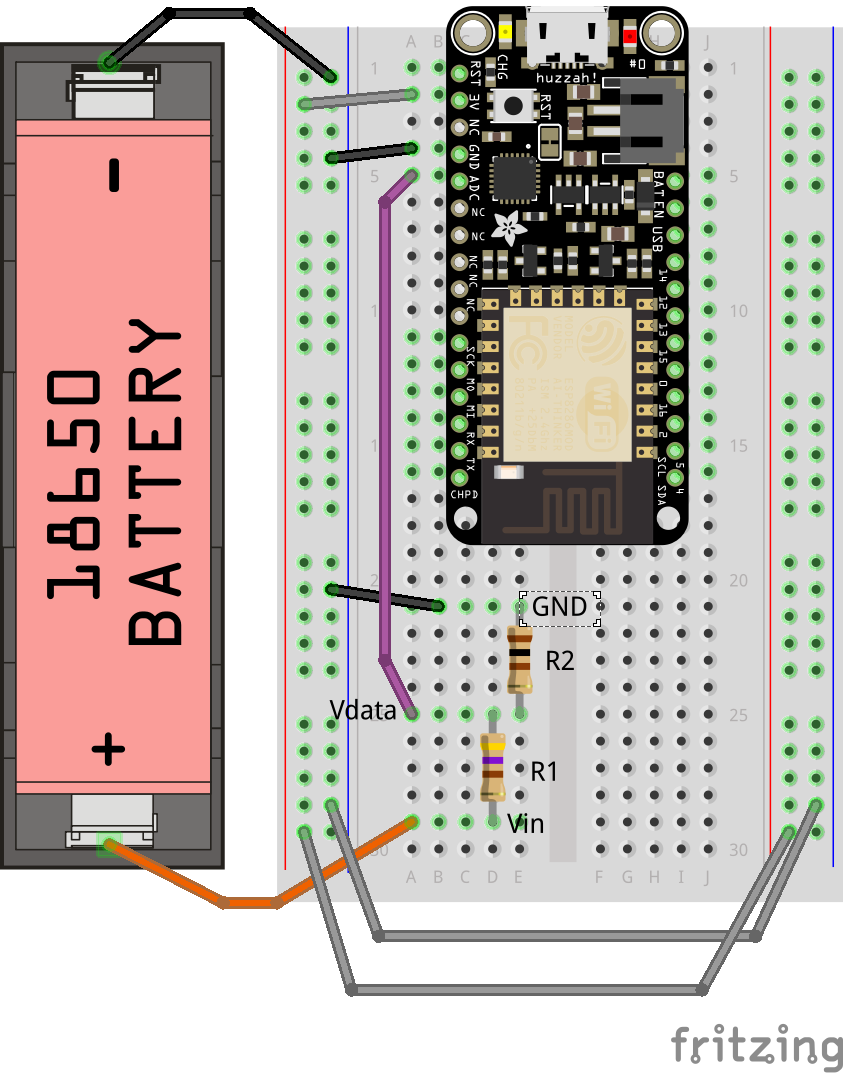
\includegraphics[width=\MFW]{Fritzing/feather_voltage_divider2_bb.png}}{https://publicsensors.org/IntroSensors/Fritzing/feather_voltage_divider2_bb.png}
		\caption[Voltage divider schematic]{An illustration of the layout for an analog voltage sensor, using a \texttt{voltage divider} to measure voltage from an \texttt{\texttt{18650}} battery. 
		In the schematic, jumpers that are not needed but may be left in place if already present are indicated in gray.}
		\labfig{feather_voltage_divider2}
	\end{center}
\end{marginfigure}
An example breadboard layout is given in \reffig{feather_voltage_divider2}. 

Here's the step-by-step (\underline{be sure to do these in order}):
\begin{enumerate}
	\item \textbf{Select, label and test the resistors $R_1$ and $R_2$.}
	
	Resistors are labeled with \htmladdnormallink{colored bands}{https://en.wikipedia.org/wiki/Electronic\_color\_code} that indicate their resistance values. 
	Online calculators, such as \htmladdnormallink{Digi-Key's Color Code Calculator}{https://www.digikey.com/en/resources/conversion-calculators/conversion-calculator-resistor-color-code-4-band} make it easy to translate these bands into numerical resistance values. 
	
	\smallskip
	Even easier is to use a multimeter.
	\begin{itemize}
		\item[$\circ$] Choose resistors for the $R_1$ and $R_2$ values you identified as yielding the best voltage divider characteristics.
		\item[$\circ$] Measure the actual resistances using the multimeter.
		\item[$\circ$] Label each resistor with a piece of tape, identifying it as to the role it will play ($R_1$ or $R_2$) and its actual resistance.		
	\end{itemize}
	By measuring and labeling, you account for the possibility that the actual resistances differ substantially from the nominal resistances.
	You also reduce the risk that you will accidentally reverse $R_1$ and $R_2$ in your circuit, which could destroy the \adc.
	
	\item \textbf{Insert your microcontroller in your breadboard, in the standard position.}	
	
	\item \textbf{Insert the resistors into the breadboard.}	
	
	\reffig{feather_voltage_divider2} shows one possible layout, but many variations are possible.
	The key requirements are that:
	\begin{itemize}
		\item[$\circ$] One end of both resistors connect by inserting into the same row.
		\item[$\circ$] The other ends of each resistor insert into otherwise empty rows.	
	\end{itemize}
	\textbf{DOUBLE CHECK THAT YOUR $R_1$ AND $R_2$ RESISTORS ARE IN THE CORRECT POSITIONS, AS INDICATED IN \reffig{feather_voltage_divider2}}.
	
	\item \textbf{Use a jumper to connect the free end of your $R_2$ resistor to the negative rail.}
	
	\item \textbf{Insert your \texttt{\texttt{18650}} battery into the battery holder, making sure to have the positive terminal of the battery in the positive end of the battery holder.}

	\item \textbf{Insert the ``\texttt{-}'' (black) wire from the battery holder into the negative rail  (\texttt{GND}).}

	\item \textbf{Insert the ``\texttt{+}'' (red) wire from the battery holder to the free end of your $R_1$ resistor  (\texttt{Vin}).}

	\item \textbf{Test your connections!}

	At this point, there is voltage across the voltage divider. 
	To insure your circuit is safe for your \texttt{ESP8266}'s \adc, confirm that: 
	\begin{itemize}
		\item[$\circ$] Voltage across the free ends of $R_1$ and $R_2$ is in the range of \texttt{+3.6} to \texttt{+4.3 volts}.
		\item[$\circ$] Voltage across $R_2$ is in the range of \texttt{0} to \texttt{+1 volts}.	
	\end{itemize}
	\textbf{IF EITHER OF THESE IS NOT TRUE, DO NOT PROCEED UNTIL YOU HAVE IDENTIFIED AND CORRECTED THE PROBLEM}.
	 
	\item \textbf{Use a jumper to connect your \texttt{ESP8266} \texttt{GND} pin to the negative rail.}
	 
	When you establish this connection, it insures that the ``zero'' voltage (\texttt{GND}) is the same for the battery, voltage divider and microcontroller.
	
	\item \textbf{Use a long jumper to connect your \texttt{ESP8266}'s \adc pin to the row with both $R_1$ and $R_2$ connections (\texttt{Vdata}).}
\end{enumerate}

	The hardware assembly is now complete.
	Now it's time for the software!
	
\begin{enumerate}[resume]
	\item \textbf{Connect a USB cable to your microcontroller, an open a \texttt{REPL} session.}
	
	\item \textbf{Create an \adc object, and use it to query the voltage of $V_{data}$.}
\begin{lstlisting}[language=Python]
from machine import ADC   # import the ADC module
adc = ADC(0)              # create an ADC object
adc.read()    # read the ADC and print the result
\end{lstlisting}	

	\item \textbf{On your laptop or desktop, write a Micropython function that prints the battery voltage, $V_{in}$.}
	
	Use the following code to define your function, replacing the example resistor values with the correct values for your voltage divider:

	\lstinputlisting[language=Python,label=BatteryVoltage,caption={\htmladdnormallink{\texttt{BatteryVoltage.py}}{https://github.com/seastate/IntroSensors/blob/main/Codes/BatteryVoltage.py}: A Python function to calculate battery voltage using the \adc and a voltage divider.}]{Codes/BatteryVoltage.py}
	
	\item \textbf{Execute your function on your microcontroller.}
	
	You can load this function either using the \texttt{<ctrl>-e/<ctrl>-d} sequence to paste it into a \texttt{REPL} session, or by transferring the file and importing it.
	Either way, the commands (with resistor values modified)
\begin{lstlisting}[language=Python]
from BatteryVoltage import battery_voltage
battery_voltage(R1=470.,R2=47.)
\end{lstlisting}	
	should now return a measurement of your \texttt{\texttt{18650}} battery voltage.	
	If you change to other resistor values, you can calculate voltage for the new voltage divider by changing the \texttt{R1} and \texttt{R2} arguments of the function.
\end{enumerate}

\loadMilestone{mlst:04b} % load milestone with tags id: mlst:04b

%\vspace{3 cm}
%\begin{itemize}
%	\item Quantities and units
%	\item Analogies with pipe flow
%	\item Ohm's Law
%	\item voltage-based analog sensors: thermistors
%	\item time-based analog sensors: sonar \& light
%\end{itemize}
%
%\begin{itemize}
%	\item multimeters
%	\item ADC on ESP8266
%	\item how-to: design a voltage divider
%	\item how-to: build a voltage divider
%\end{itemize}

\section{Environmental sensing with voltage: measure temperature with a thermistor}
\labsec{cal_therm}
A \htmladdnormallink{thermistor}{https://en.wikipedia.org/wiki/Thermistor} is an electrical component whose resistance changes with temperature.
Thermistors are readily available and inexpensive, and low cost temperature sensors made from them can have very good accuracy and precision.
Unsurprisingly, thermistors are widely used as temperature sensors in industry and household appliances. 
For example, the temperature in refrigerators and ovens are often controlled by circuits using a thermistor to sense temperature.
In this section you will design, assemble and calibrate an analog sensor using a thermistor, and use it to measure variations in environmental temperature.

The voltage divider you built in \refsec{meas_volt} was designed to measure voltage from a battery. % that was outside the \texttt{ESP8266} \adc's tolerance limits. 
In the design process, you used Ohm's Law to deduce the unknown voltage, $V_{in}$, from a known pair of resistors $R_1$ and $R_2$ and the measured output voltage, $V_{data}$.
As Equation \ref{OhmsRVI} shows, Ohm's Law has an equivalent application in deducing resistance from known voltage and current.
This suggests that, in a voltage divider where $V_{in}$ and either $R_1$ or $R_2$ are known, $V_{data}$ could be used to infer the other, unknown resistor value.
%This suggests that a voltage divider in which both $V_{in}$, $V_{data}$ and either $R_1$ or $R_2$ are known could be used to infer the other, unknown resistor value.

The analog temperature sensor you will make uses a voltage divider in this way. 
The unknown resistor in this voltage divider will be a thermistor.
Quantifying this thermistor's resistance --- combined with a calibration of how its resistance varies as a function of temperature --- will enable you to use your microcontroller to measure ambient temperature.

Using Equation \ref{vd4} as a starting point, we have two options.
We could use the thermistor to replace $R_1$.
In that case, solving Equation \ref{vd4} for $R_1 = R_{therm}$ gives us 
\begin{equation}\label{therm1}
R_{therm} = \frac{V_{in}-V_{data}}{V_{data}}R_2.
\end{equation}
Alternatively, we could use the thermistor to replace $R_2$.
Then, solving Equation \ref{vd4} for $R_2 = R_{therm}$ gives us 
\begin{equation}\label{therm2}
R_{therm} = \frac{V_{data}}{V_{in}-V_{data}}R_1.
\end{equation}
We do not know ahead of time which strategy will yield a better temperature sensor.
Which resistor to replace, and what value to choose for the remaining resistor, will emerge from the sensor design process.

\subsection{Thermistor temperature-resistance curves}
Thermistors are usually referred to by their \texttt{nominal resistance value}, which is their designed resistance at the reference temperature, $25^\circ$ \texttt{C} ($77^\circ$ \texttt{F}).
Common nominal resistance values for thermistors range from $100\Omega$ through $100k\Omega$.
Within this range are many nominal resistance values that are somewhat standard for specific purposes.
For example, many 3D printers use a $22k\Omega$ thermistor to measure the temperature at which melted plastic is being extruded to build up a part. 

The most common type of thermistor in temperature sensors is a \texttt{``negative temperature coefficient''} (\texttt{NTC}) thermistor.
In an \texttt{NTC} thermistor, the resistance is lower at higher temperatures, and higher at lower temperatures.
(The converse --- a \texttt{``positive temperature coefficient''} (\texttt{PTC}) thermistor, has higher resistance at higher temperatures, and lower resistance at lower temperatures.)
This change in resistance with temperature is what makes a thermistor suitable as the basis of a temperature sensor. 
However, it also means that we must anticipate the entire range of possible resistance values in our circuit design, to get the best possible resolution while insuring that the voltage divider will never exceed the \adc voltage tolerance.

%To evaluate alternative configurations for a voltage divider measuring thermistor resistance, we need to consider how that resistance varies over the relevant range of temperatures. 
%\texttt{NTC} means that resistance goes down with increasing temperature.  
A systematic study of temperature-resistance curves for \texttt{NTC} thermistors was published in 1968 by Steinhard and Hart \cite{STEINHART1968497}.
The formula that they found to best describe these curves is known as the \htmladdnormallink{\texttt{Steinhart-Hart equation}}{https://en.wikipedia.org/wiki/Steinhart\%E2\%80\%93Hart\_equation},
\begin{equation}\label{therm3}
\frac{1}{T_{k}} = A + B \ln R_{th} + C (\ln R_{th})^3.
\end{equation}
In this equation, $T_{k}$ is thermistor temperature in \texttt{kelvins}.
$R_{th}$ is resistance in \texttt{ohms}.
$A$, $B$ and $C$ are calibration constants --- called \texttt{Steinhart-Hart coefficients} ---  that are determined for a given thermistor by measuring its resistance at three known temperatures.
If the three calibration temperatures are $T_{k,1}$, $T_{k,2}$ and $T_{k,3}$, and the corresponding resistances are $R_1$, $R_2$ and $R_3$, then the following formulas determine $A$, $B$ and $C$:
\begin{eqnarray}
L_1 = \ln R_1, ~L_2 = \ln R_2, ~L_3 = \ln R_3  \non \\
Y_1 = \frac{1}{T_{k,1}}, ~Y_2 = \frac{1}{T_{k,2}}, ~Y_3 = \frac{1}{T_{k,3}} \non \\
\gamma_2 = \frac{Y_2-Y_1}{L_2-L_1}, \gamma_3 = \frac{Y_3-Y_1}{L_3-L_1} \non \\
C = \frac{\gamma_3-\gamma_2}{L_3-L_2} (L_1+L_2+L_3)^{-1}  \label{therm4}\\
B = \gamma_2 - C(L_1^2 + L_1 L_2 + L_2^2) \non \\
A = Y_1 - (B+L_1^2 C) L_1 \non 
\end{eqnarray}
It's sometimes useful to calculate a thermistor's resistance, $R_{th}$, from its temperature (that is, the \emph{inverse} of Equation \ref{therm3}).
One approach is through trial and error --- plugging a few guesses of $R_{th}$ into Equation \ref{therm3}), it's usually possible to come quite close to a specific $T_k$.
However, an explicit formula is available:
\begin{equation}\label{therm5}
R_{th} = e^{\left(\sqrt[3](y-x) - \sqrt[3](y+x)\right)} ,
%R_{th} = \exp\left(\sqrt[3](y-x) - \sqrt[3](y+x)\right) ,
\end{equation}
where
\begin{equation}\label{therm6}
x = \frac{1}{2C} \left( A - \frac{1}{T_{k}} \right), ~ y = \sqrt{\left(\frac{B}{3C}\right)^3+x^2}.
\end{equation}
These formulas provide the theoretical basis for calibrating your thermistor.

%http://www.aetsolar.com/literature/Manuals/TempVsResistChart.pdf

\subsubsection{\howto Calibrate a thermistor}
\labsec{therm_cal}
The first step in designing a thermistor-based temperature sensor is to calibrate its temperature-resistance curve by determining its Steinhart-Hart coefficients.
In this section, you will create simple water baths at three known temperatures $T_{k,1}$, $T_{k,2}$ and $T_{k,3}$, and use them to measure thermistor resistances $R_1$, $R_2$ and $R_3$ in Equation \ref{therm3}.

You will then use Equations \ref{therm3}--\ref{therm6} to calculate the Steinhart-Hart coefficients for your thermistor.
Establishing the Steinhart-Hart coefficients calibrates your thermistor, enabling you to calculate temperature from resistance and \textit{vice versa}.

It's worth noting that, to be good calibration temperatures, $T_{k,1}$, $T_{k,2}$ and $T_{k,3}$ should span all or most of the temperature range of interest.
Furthermore, they should ideally be spaced roughly equally apart within this range.
This is so that, to the extent possible, the Steinhart-Hart equations will be used to \texttt{interpolate} rather than \texttt{extrapolate} the temperature-resistance relationship. 
As you may have found in previous scientific work, extrapolation often magnifies small errors in calibration such that they become disproportionately large far from measured data points. 

In the calibration procedure below, we will illustrate the steps using example values from a $10k\Omega$ thermistor. 
Substitute the values you obtain from your thermistor into these calculations.
\begin{enumerate}
	\item \textbf{Prepare water baths at three different temperatures.}
	
	Typically, most laboratory thermometers give temperature in $^\circ$ \texttt{Celsius}.
	Remember that temperature in Celsius, $T_c$, is related to $T_k$ by 
	\begin{equation*}
		T_k = T_c + 273.15, ~T_c = T_k - 273.15.
	\end{equation*}
	To use water bath temperatures measured in \texttt{Celsius} for thermistor calibration, you must either convert them to $^\circ$ \texttt{Kelvin} using the formula above, or use the version of the Python scripts below that does that conversion for you.
	
	\smallskip
%	To be good calibration temperatures, $T_{k,1}$, $T_{k,2}$ and $T_{k,3}$ should span all or most of the temperature range of interest, and be spaced roughly equally apart within this range.
	In most classrooms and laboratories, three suitable temperatures that are easy to produce in water baths are:
	\begin{itemize}
		\item[$\circ$] $0^\circ$ \texttt{C}, which is the equilibruim temperature of a mixture of frozen and liquid fresh water. 		
		\item[$\circ$] $100^\circ$ \texttt{C}, which is the boiling temperature of a cup of fresh water. 
		\item[$\circ$] Room temperature, which is usually close to $25^\circ$ \texttt{C}.
%  Human body temp: $36.5–37.5^\circ$ \texttt{C}		
	\end{itemize} 

	A good way to create ``water baths'' at these three temperatures for thermistor calibration is with paper bowls or cups, filled with a water/ice mixture, boiling water and room temperature water.
	Cover each bath with a lid, so that it maintains its temperature for longer and does not cool through evaporation. 
	Confirm the actual temperatures of your water baths with the most accurate thermometer you can find, e.g. by inserting it through a small hole in the lid.
	
	\item \textbf{Prepare your thermistor for resistance measurements.}
	
	The goal in this step is to enable you to measure resistance across the thermistor with a multimeter, while that thermistor is held at known temperatures by the water baths.
	We leave it to your ingenuity to come up with effective, creative solutions to the materials you have on hand. 
	
	\smallskip
	We'll illustrate with two examples, both of which are inexpensive and easily obtained $10k\Omega$ thermistors.\todo{pictures of Thermistors A and B}
	However, many other thermistor types and water bath arrangements are workable.
	\begin{itemize}
		\item[$\circ$] \texttt{Thermistor A} is a ``bead'' thermistor, with two bare wires.
		This kind of thermistor responds quickly to temperature changes, but is not protected from water or other corrosive or conductive liquids.
		
		\smallskip
		To calibrate \texttt{Thermistor A}, use removable tape (like painter's masking tape) to attach it snugly to the outside of the water baths
		It should directly touch the surface of the water bath, to conduct heat as quickly as possible from the water bath surface. 
		Then, cover the thermistor with a layer of foam or folded paper towels to insulate it from the surrounding air.
		Keep in mind that the wires can conduct heat into or out of the thermistor, so ideally they will also be in contact with the bath and covered by the insulation.
		%Be sure, though, to leave enough of the wires exposed to connect to multimeter leads to measure resistance.
		 		
		\item[$\circ$] \texttt{Thermistor B} is ``potted'', meaning it is encased in a protective stainless steel sleeve, and embedded in epoxy or some other sealant. 
		This casing means that the thermistor is waterproof --- it can be submerged directly into the water baths.
		However, because the casing retains a significant amount of heat, potted sensors can be slower to respond to temperature changes than bead thermistors.

		\smallskip
		To calibrate \texttt{Thermistor B}, immerse the thermistor entirely within the water bath, with its wires coming out through a small hole in the lid.

	\end{itemize} 

	\item \textbf{Measure resistance at each water bath temperature with a multimeter.}

	In making these measurements, keep in mind:
	\begin{itemize}
		\item[$\circ$] The \texttt{equilibration time} of the thermistor. 
		This is the time it takes for the interior of the thermistor to equalize in temperature with the surface of the water bath.
		You can get an estimate of the equilibration time by watching the resistance measured on a multimeter change immediately after you place the thermistor in contact with a surface of different temperature. 
		Typical equilibration times range from a few seconds to several minutes.
		\item[$\circ$] %Multimeters also have internal equilibration times. 
		Some multimeters have a significant amount of measurement noise, especially for very low or very high resistance values. 
		When making your measurements, wait until the resistance value appears to stabilize. 
		Then, record the resistance value at five times, spaced several seconds apart. 
		Take the median of these as the most accurate resistance measurement. 
	\end{itemize}	
	
	\item \textbf{Calculate the Steinhart-Hart coefficients.}
	
	The Python functions below enable you to calculate the Steinhart-Hart coefficients for your thermistor.
	To use them, substitute your measured temperature and resistance values for the default \texttt{T}'s and \texttt{R}'s.
	You may run these functions on your computer or, using the \texttt{<ctrl>-e / <ctrl>-d} technique, copy and run them on your microcontroller.
	
	\smallskip
	Use \lstinline{SH_coeffs_kelvins} if your temperatures are in $^\circ$\texttt{Kelvin}, and \lstinline{SH_coeffs_celsius} if your temperatures are in $^\circ$\texttt{Celsius}. Both functions return the Steinhart-Hart coefficients \lstinline{(A, B, C)} as a Python tuple.
	\lstinputlisting[language=Python,label=SteinhartHart,caption={\htmladdnormallink{\texttt{SteinhartHart.py}}{https://github.com/seastate/IntroSensors/blob/main/Codes/SteinhartHart.py}: Python functions to calculate Steinhart-Hart coefficients for thermistor calibration.}]{Codes/SteinhartHart.py}
	
	
	\item \textbf{Verify the resistor and temperature calculations.}
	
	The Python functions below calculate temperature from resistance and \textit{vice versa} for a calibrated thermistor.
	\lstinputlisting[language=Python,label=thermistor,caption={\htmladdnormallink{\texttt{thermistor.py}}{https://github.com/seastate/IntroSensors/blob/main/Codes/thermistor.py}: Python functions to calculate temperature from resistance and \textit{vice versa} for a calibrated thermistor.}]{Codes/thermistor.py}
	As an initial test, try calculations with your known values: $R_1$ from $T_{k,1}$, $T_{k,2}$ from $R_2$, \etc
	For \emph{consistency}, you should get the same result as you entered for your calibration.
	
	\smallskip
	Next, use both a thermometer and your thermistor to measure another temperature, e.g. outside or in an unheated storage space, or in a water bath at a new temperature. 
	What is the percent error between the thermometer and your thermistor temperature readings? 
	
\end{enumerate}
\loadMilestone{mlst:04c} % load milestone with tags id: mlst:04c


\subsection{Thermistor circuit design}
To design a circuit that effectively uses a thermistor to measure environmental temperatures, you will use the tools you developed in the last two sections: A calibration enabling you to calculate your thermistor's resistance across the relevant range of temperatures, and a spreadsheet enabling you to calculate which resistor combinations satisfy the \texttt{ESP8266}'s \adc voltage tolerance.

There are two circuit configurations that you need to consider:
\begin{itemize}
	\item Configuration 1, in which the thermistor replaces resistor $R_1$ from the voltage divider circuit:
	\begin{figure}[H]
	\begin{center}
		\begin{tikzpicture}[american voltages]
		\draw
		(0,0) to [short,l=$V_{in}$, *-] (1,0)
		to [thRn, l=$RTH_1$] (3,0)
		to [short, i_=$I$,l=$V_{data}$] (4,0)
		to [R, l=$R_2$] (6,0)
		to [short,l=GND, -*] (7,0);
		\end{tikzpicture}
		\caption[Thermistor circuit \#1]{Schematic diagram of a voltage divider circuit, with the thermistor replacing resistor $R_1$.}
		\labfig{therm_cir1}
	\end{center}
	\end{figure}

	\item Configuration 2, in which the thermistor replaces resistor $R_2$ from the voltage divider circuit:
	\begin{figure}[H]
	\begin{center}
		\begin{tikzpicture}[american voltages]
		\draw
		(0,0) to [short,l=$V_{in}$, *-] (1,0)
		to [R, l=$R_1$] (3,0)
		to [short, i_=$I$,l=$V_{data}$] (4,0)
		to [thRn, l=$RTH_2$] (6,0)
		to [short,l=GND, -*] (7,0);
		\end{tikzpicture}
		\caption[Thermistor circuit \#2]{Schematic diagram of a voltage divider circuit, with the thermistor replacing resistor $R_2$.}
		\labfig{therm_cir2}
	\end{center}
	\end{figure}
\end{itemize}
In these circuit diagrams, the box with the diagonal line represents the thermistor, in which resistance is modulated by temperature. We have labeled the thermistor in these positions $RTH_1$ and $RTH_2$, to remind us that these thermistors replace resistors $R_1$ and $R_2$, respectively, in our voltage divider calculations.

\subsubsection{\howto Design a voltage divider for a thermistor}
\labsec{therm_des}
\begin{enumerate}
	\item \textbf{Make two copies of the voltage divider calculations spreadsheet from \refsec{vd_design}.}
	
	Save one with a name that includes something like ``\texttt{RTH1}''. You'll use this one to make calculations for Configuration 1.
	Likewise, save the other with an informative name that includes something like ``\texttt{RTH2}''. 
	
	\item \textbf{Modify the \texttt{RTH1} spreadsheet for the thermistor circuit.}
	
	Starting with the voltage divider spreadsheet:
	\begin{itemize}
		\item[$\circ$] \textbf{Change the entries under the \texttt{Vin} column heading to \texttt{3.3}.} 
		This reflects the fact that we will use the \texttt{3V3} pin to power the thermistor circuit. This pin always outputs exactly \texttt{3.3 volts}.
		
%		\item[$\circ$] Change the logical test in the fifth column to read \lstinline{R2<=R1/2.3?}. Then, change the formula in the rest of the fifth column to read \lstinline{=C2<(B2/2.3)}. This reflects the criterion on resistances to meet the voltage tolerance with the $V_{in}=3.3$ \texttt{volts}.
%		 
		\item[$\circ$] \textbf{In the top row, change the \texttt{R1} column header to \texttt{RTH1}.}
				 
		For neatness, make the same change in the \texttt{R2/R1} header, to \texttt{R2/RTH1}.
		\item[$\circ$] \textbf{In the top row under the \texttt{RTH1} column header, enter the thermistor resistance you measured at the lowest temperature, $0^\circ$\texttt{C}.} 
		\item[$\circ$] \textbf{In the next row, replace the \texttt{RTH1} column resistance with the thermistor resistance you measured at the highest temperature, $100^\circ$\texttt{C}.} 
		These represent the whole range of resistances that can occur in the voltage divider within the calibrated interval, $0-100^\circ$\texttt{C}. 

		\item[$\circ$] \textbf{Copy a candidate $R_2$ resistor value into \underline{both} rows under the \texttt{R2} column.}
		
		Your spreadsheet rows will then look something like this (using $R_2=100\Omega$ resistors as an example):
\begin{table}[H]
	\centering
	\begin{small}
		\begin{tabular}{|c|c|c|c|c|c|c|c|c|}
		\hline 
			\textbf{A}  & \textbf{B} & \textbf{C} & \textbf{D} & \textbf{E} & \textbf{F} & \textbf{G} & \textbf{H} & \textbf{I} \\ 
			\hline 
			Vin  & RTH1 & R2 & R2/RTH1 & Vdata & Vdata<1? & I & W & Vres \\ 
			\hline 
			3.3 & 32648  & 100 & 3.06E-03 & 1.01E-02 & TRUE & 1.01E-04 & 3.33E-04 & 3.20E-01 \\ 
			\hline 
			3.3 & 680  & 100 & 1.47E-01 & 4.23E-01 & TRUE & 4.23E-03 & 1.40E-02 & 7.62E-03 \\ 
			\hline 
		\end{tabular} 
	\end{small}
\end{table}

%		\item[$\circ$] \textbf{Examine the results in the remaining }
	
	\end{itemize}


	\item \textbf{Calculate ``self-heating'' of the thermistor due to dissipated electrical energy.}

	In the ``\texttt{W}'' column of your spreadsheet, you calculate the rate at which electrical power is lost to heat in the voltage divider. 
	This is an important piece of information, because high rates of power dissipation can discharge the battery faster than necessary.
	
	\smallskip
	In our thermistor circuit, however, power dissipated to heat plays another role --- it heats the temperature sensor!
	If the thermistor itself is generating a substantial amount of heat, that could cause artifacts in its temperature readings. 

	\smallskip
	To calculate the heat generation inside the thermistor, $W_{th}$, we can again use Equation \ref{watts}.
	Because we have already calculated the current, $I$, the simplest approach is to calculate $W_{th}$ as the product of $I^2$ and thermistor resistance.
\begin{itemize}
	\item[$\circ$] \textbf{Add a column header, \texttt{WTH1}, in the column after \texttt{Vres}.}
	\item[$\circ$] \textbf{Enter the formula \lstinline{=(H2^2)*B2} into the cells below \texttt{WTH1}.}
\end{itemize}
	Your spreadsheet will now look something like this: 
\begin{table}[H]
	\centering
	\begin{small}
		\begin{tabular}{|c|c|c|c|c|c|c|c|c|c|}
			\hline 
			\textbf{A}  & \textbf{B} & \textbf{C} & \textbf{D} & \textbf{E} & \textbf{F} & \textbf{G} & \textbf{H} & \textbf{I} & \textbf{J} \\ 
			\hline 
			Vin  & RTH1 & R2 & R2/RTH1 & Vdata & Vdata<1? & I & W & Vres & WTH1\\ 
			\hline 
			3.3 & 32648  & 100 & 3.06E-03 & 1.01E-02 & TRUE & 1.01E-04 & 3.33E-04 & 3.20E-01 & 3.32E-04\\ 
			\hline 
			3.3 & 680  & 100 & 1.47E-01 & 4.23E-01 & TRUE & 4.23E-03 & 1.40E-02 & 7.62E-03 & 1.22E-02\\ 
			\hline 
		\end{tabular} 
	\end{small}
\end{table}
	where the last column is the heat (in \texttt{watts}) generated in the thermistor.
	
	\item \textbf{Explore alternative resistor values, by making copies of the two rows of calculations, and entering different values for \texttt{R2}.}
	
	Does the new resistance value satisfy the \adc voltage tolerance?\sidenote[][*-25]{
		\begin{kaobox}[backgroundcolor=\SNcolor,frametitlebackgroundcolor=\SNcolor,frametitle=Resist-metic]As we found in the voltage divider discussion, the total resistance of two resistors connected in \emph{series} (one connected end to end with the other) is simply the sum of their individual resistances: $R_{total}=R_1+R_2$. 
			You can use this fact if you want to use a resistor value that you don't have in hand. 
			For example, if you have $510\Omega$ and $220\Omega$ resistors, you can attach them in series to form a $510+220=730\Omega$ resistor.	 	
		\end{kaobox}
	} 
	Is the resolution better or worse with new \texttt{R2} resistances?
	Are the total power dissipation and the heat generated inside the thermistor larger or smaller than the previous \texttt{R2} choices?
	
	\item \textbf{Repeat all the above steps for the \texttt{RTH2} spreadsheet, but this time replacing \texttt{R2} with \texttt{RTH2}.}
	
	In this case, the formula for \texttt{WTH2} is \lstinline{=(H2^2)*C2}.
	The result (using $R_1=100k\Omega$ as an example) will be similar to:
\begin{table}[H]
	\centering
	\begin{small}
		\begin{tabular}{|c|c|c|c|c|c|c|c|c|c|}
			\hline 
			\textbf{A}  & \textbf{B} & \textbf{C} & \textbf{D} & \textbf{E} & \textbf{F} & \textbf{G} & \textbf{H} & \textbf{I} & \textbf{J} \\ 
			\hline 
			Vin  & R1 & RTH2 & RTH2/R1 & Vdata & Vdata<1? & I & W & Vres & WTH2\\ 
			\hline 
			3.3 & 1.00E+05  & 32648 & 3.26E-01 & 8.12E-01 & TRUE & 2.49E-05 & 8.21E-05 & 9.37E-03 & 2.02E-05\\ 
			\hline 
			3.3 & 1.00E+05  & 680 & 6.80E-03 & 2.23E-02 & TRUE & 3.28E-05 & 1.08E-04 & 1.45E-01 & 7.31E-07\\ 
			\hline 
		\end{tabular} 
	\end{small}
\end{table}	
	
\end{enumerate}
\loadMilestone{mlst:04d} % load milestone with tags id: mlst:04c


\subsection{Thermistor circuit assembly and programming}
Laying out and assembling a voltage dividing circuit to measure temperature with a thermistor requires only a few changes from the voltage divider you built in \refsec{vd_assem}.
Then, measuring temperature involves three steps that happen in Python scripts:   
\begin{itemize}
	\item Use the \adc to measure $V_{data}$.
	\item Use Equation \ref{therm1} or \ref{therm2} (depending on your circuit configuration) to infer the thermistor resistance $R_{therm}$ from $V_{data}$.
	\item Use your thermistor calibration from \refsec{therm_cal} to infer temperature from $R_{therm}$.
\end{itemize} 
The following \textit{HOW-TO} takes you through these steps. 
 
\subsubsection{\howto Build and test a thermistor circuit}
If you have chosen Configuration 2, your circuit layout will be similar to \reffig{feather_thermistor}.
If you have chosen Configuration 1, your circuit layout will have the thermistor in position \texttt{R1} rather than \texttt{R2}, but be otherwise similar to \reffig{feather_thermistor}.

\labsec{therm_build}
\begin{marginfigure}[-8cm]
	\begin{center}
		\htmladdnormallink{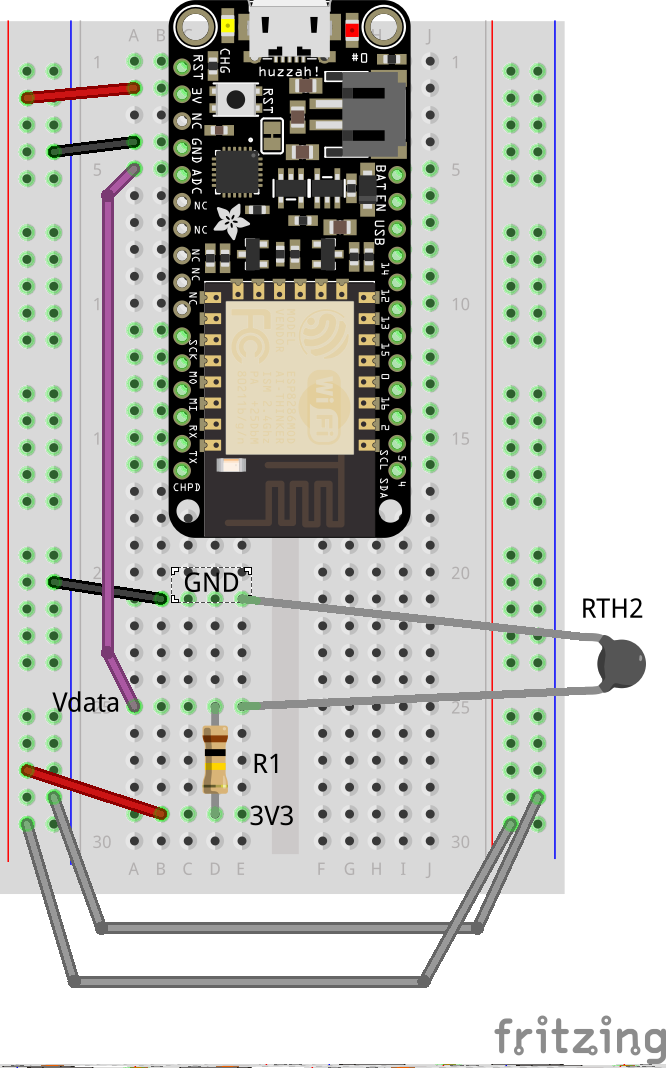
\includegraphics[width=\MFW]{Fritzing/feather_thermistor_bb.png}}{https://publicsensors.org/IntroSensors/Fritzing/feather_thermistor_bb.png}
		\caption[Thermistor circuit schematic]{An illustration of the layout for a circuit using a thermistor to measure temperature. 
		This schematic represents Configuration 2, in which the thermistor (here labeled \texttt{RTH2}) takes the place of resistor $R_2$ in the original voltage divider circuit.
		In Configuration 1, the thermistor would instead take the place of resistor $R_1$. 
		In the schematic, jumpers that are not needed but may be left in place if already present are indicated in gray.}
		\labfig{feather_thermistor}
	\end{center}
\end{marginfigure}
\begin{enumerate}
	\item \textbf{Disconnect your microcontroller from USB power.}
	
	\item \textbf{If you are modifying the battery voltage circuit, disconnect one end of the jumper to the \adc.}
	
	Both these precautions are to prevent accidentally exposing your \adc to voltages higher than its tolerance, while you build and check your circuit. 

	\item \textbf{Assemble and double check the thermistor circuit.}

Compared to the battery voltage circuit, the changes are:
	\begin{itemize}
		\item[$\circ$] Use a jumper to connect the power rail to the open end of resistor \texttt{R1} (or \texttt{RTH1} if you are using Configuration 1).
		
		The power rail, which is connected to the \texttt{ESP8266}'s \texttt{3V3} pin, supplies positive voltage (instead of the battery in the original circuit). 
		\item[$\circ$] \textbf{Replace the appropriate resistor (\texttt{R1} for Configuration 1, \texttt{R2} for Configuration 2) with the thermistor.} 
		\item[$\circ$] \textbf{Replace the other resistor (\texttt{R2} for Configuration 1, \texttt{R1} for Configuration 2) with the resistor you chose in your design analysis in \refsec{therm_des}.}
	\end{itemize}	

	\item \textbf{With the \adc jumper still disconnected, plug the microcontroller into USB power.}
		
	\item \textbf{Use a multimeter to check that voltage $0 \le V_{data} \le 1$.}
	
	At this point, the voltage divider should be powered up and operating as it would during temperature measurements.
	
	\smallskip
	IF THE CONDITION $0 \le V_{data} \le 1$ IS NOT MET, STOP AND DEBUG YOUR CIRCUIT.
	
	\smallskip
	Do not proceed until you've diagnosed and fixed the problem in the circuit --- it could destroy the \adc.

	\item \textbf{Connect the \adc-\texttt{Vdata} jumper.}
		
\end{enumerate}
That's it for the hardware.
Now for the software!

\begin{enumerate}[resume]
	\item \textbf{Make a copy of the Python script }\lstinline{BatteryVoltage.py} \textbf{from \refsec{vd_assem}, and save it with an informative name such as as }\lstinline{ThermResist.py}\textbf{.}
	
	\item \textbf{Modify this script so that it calculates thermistor resistance.}
	
	The necessary changes are:
	\begin{itemize}
		\item[$\circ$] Change the name of the \lstinline{battery_voltage} function to an informative name, e.g. \lstinline{therm_resistRTH2} if you are using Configuration 2. 
		
		\item[$\circ$] \textbf{Change the \texttt{arguments} of the function from the parameters in the original voltage divider,} \lstinline{R1=470.,R2=47.}\textbf{, to the parameters in the thermistor circuit:} \lstinline{R1=1.e5,vin=3.3}\textbf{.} 
		
		\item[$\circ$] \textbf{Replace the calculation of $V_{in}$ in line 4, with calculation of \texttt{RTH1} or \texttt{RTH2} from Equation \ref{therm1} or \ref{therm2}.}
	
		\item[$\circ$] Replace \texttt{vin} in the \texttt{return} statement with \texttt{RTH1} or \texttt{RTH2}.
	\end{itemize}
	
	\item \textbf{Save your changes, copy onto your microcontroller, and test the script.}

	To test, call the function with the resistor value that corresponds to your circuit,
\begin{lstlisting}[language=Python]
rth2=therm_resistRTH2(R1=1.e5,vin=3.3)
T=thermistor_temp_celsius(Rth=rth2,A=0.,B=0.,C=0.)
print('Thermistor temperature = ',T)
\end{lstlisting}	
	In the call to the \lstinline{thermistor_temp_celsius} function, remember to assign the correct values to $A$, $B$ and $C$ according to the calibration you obtained in \refsec{therm_cal}.
	
	
\end{enumerate}
\loadMilestone{mlst:04e} % load milestone with tags id: mlst:04e

%
%\vspace{4cm}
%\begin{itemize}
%	\item temperature-resistance curves
%	\item measuring resistance with a voltage divider
%	\item design and assembly of a thermister-based voltage divider
%	\item calibration and coding for thermister-based temperature measurements
%	\item refining the thermistor circuit using Kirchhoff's Law's 
%\end{itemize}


\section{Environmental sensing with time: measuring light intensity with frequency}
\labsec{light_freq}
Light is a key variable in the physics, chemistry and biology of most terrestrial and marine environments. 
Light is an interesting and complex environmental characteristic in part because of its variable effects across the UV, visible and IR ranges of the electromagnetic spectrum, and because its intensity varies many orders of magnitude over short time and space scales.
These properties also make light a challenge to measure.

Sensors are widely available that respond to light by varying resistance, analogous to thermistors' responses to temperature.
An example is a \htmladdnormallink{photoresistor}{https://en.wikipedia.org/wiki/Photoresistor}.
We could therefore measure light with a voltage divider incorporating a photoresistor, using a very similar approach to calibration and implementation as for the thermistor voltage divider. 

In this section, we will instead use an analog sensor that signals light levels using time --- specifically, the frequency of electrical pulses --- rather than voltage. 
Your \texttt{ESP8266}, like many microcontrollers, can measure time intervals with relatively high resolution over a much larger range of magnitudes than its \adc can measure voltage. 
As you might expect, this broad measurement range means that time-based sensors enable the \texttt{ESP8266} to quantify light with similarly higher resolution and larger intensity range, compared to voltage-based sensors.

To compound this advantage, it is very easy (using components designed for the purpose) to ``\emph{divide}'' a frequency signal -- that is, to reduce its frequency by a standard factor of 8 or 10. 
If a sensor frequency approaches the upper limits of a microcontroller's measurement capabilities, dividing the signal in this way provides a reduced frequency that is within the microcontroller's limits. 
It is then easy to convert the reduced frequency back to the original, with multiplication by the same factor.

To take advantage of this increase in sensor range, the circuit you will build will have two sub-circuits: One measures frequency directly from the light sensor.
The other measures the reduced frequency output from a divider. 
As part of the sensor design, you will determine a suitable criterion for choosing which sub-circuit's measurements are most accurate at different light levels.

\subsection{Measuring light with frequency}
The sensor you will use in this circuit is the \htmladdnormallink{TSL237 High-Sensitivity Light-to-Frequency Converter}{https://ams.com/documents/20143/36005/TSL237\_DS000156\_3-00.pdf/4aa35672-5c5e-3bb7-4d6b-92f4c76a3531}.
Like most of the analog sensors we've considered, this sensor has three wires.
Two are the usual inputs, $GND$ and $V_{in}$. 
The third is the output, $V_{data}$, which oscillates between $GND$ and $V_{in}$ at a frequency, $f$, proportional to light intensity.

Important information about this sensor is contained in the \texttt{datasheet} linked above.
The oscillation frequency in absolute darkness, $f_{dark}$, is typically around \texttt{0.1 Hz} (it varies somewhat with temperature).
The ``\texttt{full-scale frequency}'' --- the highest frequency that can be put out by the sensor --- is $f_{full}=1000kHz=1MHz$.
Figure 9 in the datasheet shows how irradiance, $E$, varies with frequency across more than 5 orders of magnitude in both quantities.

The responsiveness of the \texttt{TSK237} sensor varies with wavelength of the incident light, at maximum near 700nm and dropping to half the maximum at approximately 400nm and 875nm (Figure 10 of the datasheet).
Figures 13 and 14 show how responsiveness varies with the angle of the incident light --- it has relatively high responsiveness ($>75\%$) within roughly $30^\circ$ of the sensor's centerline.

Both color and angular variation (which are present for nearly all light sensors) often introduce some complications in interpretation of light intensity data in a specific location.
For example, across depth in an ocean or lake, the ambient light usually becomes bluer, as redder light is more quickly absorbed.
Depending on scattering by particles, the angular distribution of light rays may also broaden substantially.
Under a forest canopy, much of the ambient light might be in the green part of the spectrum which contributes little to photosynthesis.
In environments like these, understanding the dynamics of light may require separate measurements at different parts of the color spectrum and different angles.

With all these caveats in mind, we can see from the datasheet that the irradiance responsivity of the \texttt{TSL237} sensor is $R_e=2.3 \frac{\mathtt{kHz}}{\mathtt{uW}/\mathtt{cm}^2}$.
This implies that a \emph{nominal irradiance} --- subject to corrections for wavelength, angle and temperature --- is given by
\begin{equation}\label{irrad}
E_e = R_e (f-f_{dark}) .
\end{equation}
Equation \ref{irrad} gives us an approximate way to calibrate irradiation as a function of frequency, and to predict frequency for specific irradiances.
Because $f_{dark}$ is very small compared to $f$ in all but nearly absolute darkness, and because the errors associated with wavelength, angle and temperature are typically much larger, we can usually neglect the $f_{dark}$ term in Equation \ref{irrad}.
In that case we can simplify to a proportionality,
\begin{equation}\label{irrad2}
E_e \approx R_e f .
\end{equation}

 
\subsubsection{\howto Assemble and test a frequency-based light sensor circuit}
\labsec{tsl237}
\begin{marginfigure}[-4cm]
	\begin{center}
		\htmladdnormallink{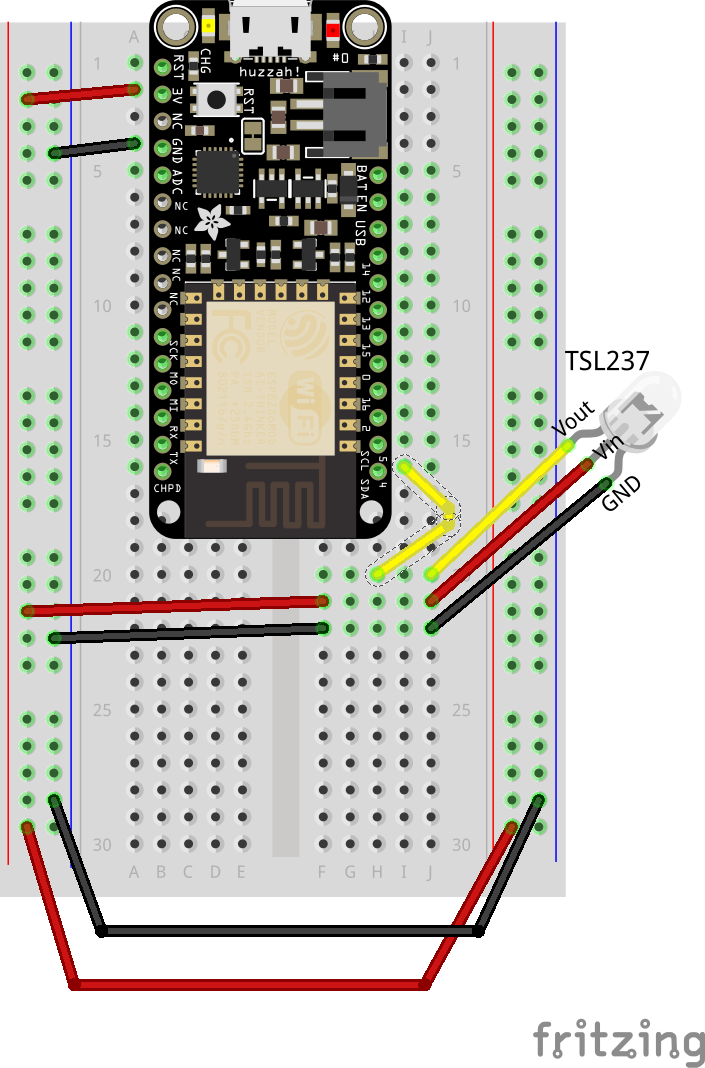
\includegraphics[width=\MFW]{Fritzing/feather_tsl237module1_bb.png}}{https://publicsensors.org/IntroSensors/Fritzing/feather_tsl237module1_bb.png}
		\caption[Light sensor sub-circuit 1 schematic]{An illustration of the circuit layout for sensing light using a \texttt{TSL237} Light-to-Frequency sensor. 
		This schematic represents sub-circuit 1, in which frequency is read directly from the sensor.
		The sensor, labeled \texttt{TSL237}, is represented by an image of an \texttt{LED}, because no image of the \texttt{TSL237} is currently available in the Fritzing software.  
		The 8 bottom rows on the breadboard are left open to leave room for sub-circuit 2. 
		Red wires represent \texttt{3.3 volts}, black wires represent \texttt{GND}, and yellow wires represent the frequency-modulated sensor output.}
		\labfig{feather_tsl237module1}
	\end{center}
\end{marginfigure}
An example layout of the \texttt{TSK237} sub-circuit is shown in \reffig{feather_tsl237module1}.



\begin{enumerate}
	\item \textbf{Starting with the \texttt{ESP8266} and power/ground rails in their usual configurations, connect the \texttt{Vin} and \texttt{GND} pins to their respective rails.}
	
	The pin assignments for the \texttt{TSL237} are shown in Figure 3 of the datasheet.
	With the sensor facing upwards (the little plastic focusing hemisphere pointing up) and wires pointing towards you, \texttt{GND} is the left wire, \texttt{Vin} is the middle wire, and \texttt{Vout} is the right wire.

	\smallskip
	In the schematic, we've illustrated jumpers between the sensor and the breadboard.
	These are to make clear how the inputs and output are connected. 
	These jumpers are optional --- you may connect the sensor directly into the breadboard, or use female-male jumpers between the sensor and the breadboard.
	
%	\smallskip
%	Very long wires between the sensor and the microcontroller can affect the sensor reading.
%	So, it's best to restrict these wires to about the length of standard jumpers.	

	\item \textbf{Connect the sensor's \texttt{Vout} to \texttt{Pin 4} on the microcontroller.}
	
\end{enumerate}
The hardware for sub-circuit 1 is now complete.

\smallskip
To measure frequency from the \texttt{TSL237} sensor, we will use a modification of code posted on the \htmladdnormallink{MicroPython forum}{https://forum.micropython.org/viewtopic.php?f=18\&t=5724\&p=32921}:
\lstinputlisting[language=Python,label=FrequencyMedian,caption={\htmladdnormallink{\texttt{frequency\textunderscore median.py}}{https://github.com/seastate/IntroSensors/blob/main/Codes/frequency_median.py}: A Python function to calculate the period of an oscillating voltage.}]{Codes/frequency_median.py}
This code uses a \Micropython \, utility called \lstinline{time_pulse_us} to measure the time, in microseconds, for a complete high/low cycle of oscillating voltage on \texttt{Pin p}.

To improve precision, the code repeats this measurement \texttt{n} times, and returns the median value. 
It also returns \texttt{True} if the measurements completed without errors.
This result is presented as a Python tuple, \lstinline{(per,valid)}, where \lstinline{per} is the measured period in $\mu s$ and \lstinline{valid} is \texttt{True} for a successful measurement.

One thing to notice about the \lstinline{time_pulse_us} function is that, if the pin it is monitoring does not change state within the interval \texttt{timeout}, an error is triggered.
In this case, \lstinline{time_pulse_us} returns \texttt{-1} or \texttt{-2} as an error message.
Two things happen if an error is returned.
The \lstinline{median_of_n} code returns \texttt{False} for \lstinline{valid}, flagging the error status.
Also, the  \lstinline{median_of_n} code returns the value of \texttt{timeout} for \lstinline{per}, instead of a measured period. 

That is, \lstinline{median_of_n} code returns the \emph{either} the measured pulse interval \emph{or} the parameter \texttt{timeout}, whichever is lower.
The code is designed this way for two reasons.
One is to prevent these error messages from contaminating frequency estimates from the light sensor. Spurious measurements of \texttt{-1} or \texttt{-2}, if treated like true measurements, would erroneously reduce the reported period and increase the inferred light intensity.
The other is to prevent the frequency measurement from being stuck for an indefinite period if there are no pulses, if the sensor is damaged or sees very low light intensity.

\smallskip
In other words, \texttt{timeout} is the maximum value for the period reported by \lstinline{median_of_n}, even if the true period is longer.
This is something to keep in mind as you assess the sensor measurements.

\begin{enumerate}[resume]
	\item \textbf{Test your light sensor circuit using the commands:}
\begin{lstlisting}[language=Python]
from frequency_median import median_of_n
from machine import Pin
p4 = Pin(4, Pin.IN)
timeout=300000
nrep=7
median_of_n(p4,nrep,timeout,verbose=True)
\end{lstlisting}	
	These commands first import the necessary modules.
	In your circuit, \texttt{Vout} from the \texttt{TSL237} is attached to \texttt{Pin 4}, so this pin is initialized as \texttt{p4} and used in the function call.
	The parameter \texttt{timeout} is here set to \texttt{300000 us}, or \texttt{0.3 s}.
	The measurement is repeated \texttt{nrep=7} times.
	In this example, \texttt{verbose=True} is used to print out the individual measurements.
	The results will be similar to
\begin{lstlisting}[language=Python]
52 [41, 51, 52, 52, 53, 54, 54]
(52, True)
\end{lstlisting}		
	This gives you a sense for the precision of successive measurements, under essentially constant ambient light conditions.
	 	
	\item \textbf{Take several measurements under different light conditions (e.g. shade the sensor with your hand, and shine a bright light directly on it).}
	
	Enter the results from \lstinline{median_of_n} in one column of a spreadsheet, under the column header \texttt{Period}.
	
	\smallskip
	In the next column, enter the header \texttt{Frequency}.
	Next each entry in \texttt{Period}, enter the formula to calculate 1000000/\texttt{Period}.
	Because \lstinline{median_of_n} measures time in microseconds, this quotient is the frequency of the signal in \texttt{herz} (cycles per second).
	
	\item \textbf{Critically assess your observations.}
	
	What is the largest and smallest period and frequency you observe in your tests?
	Do you see any evidence of limits to the range of the \texttt{TSL237}/\texttt{ESP8266} combination, either at high or low light intensities?
\end{enumerate}

\loadMilestone{mlst:04f} % load milestone with tags id: mlst:04f
%A ``driver'' is code designed to interface with a piece of hardware. 
%In the case of your light sensor, a driver should be a function that provides a clear and intuitive way to measure light. 
%\ref{irrad}

\subsection{Dividing frequency to increase sensor range}
\labsec{divider}
The sub-circuit you set up to measure light in \refsec{tsl237} should work well over a range of light conditions. 
However, there are limits to this range.
At very low light levels, readings from the sensor are limited by the parameter \texttt{timeout}, which the longest pulse interval that can be measured by the \lstinline{median_of_n} script.

At very high light levels, readings are limited by the microcontroller hardware.
The \lstinline{time_pulse_us} function cannot accurately measure intervals shorter than a few microseconds.
The \texttt{tsl237} light sensor gives a frequency up to 1 $MHz$.
This corresponds to a 1 $\mu s$ pulse interval, which is much too short for the \texttt{ESP8266} to resolve. 

How can we increase the range of light levels over which meaningful measurements can be taken by your \texttt{TSL237}/\texttt{ESP8266} instrument?
One approach is to add an additional sub-circuit to the existing circuit, that implements a counter/divider, called a \htmladdnormallink{CD4017B} {https://www.ti.com/lit/ds/symlink/cd4017b.pdf}.
The \texttt{CD4017B} takes in an input frequency, and outputs a frequency reduced by a factor of 10.
Some periods in \texttt{TSL237} output that are too short for the \texttt{ESP8266} to measure directly can be measured after being ``lengthened'' by  a factor of 10. 
This significantly extends the range of your instrument into higher light intensities. 

However, there is a tradeoff:
The longest period which can be measured is also reduced by a factor of 10, meaning that the range of the instrument is reduced at lower light intensities.
Also, its resolution is reduced by a factor of 10.

Clearly, the ideal would be the best of both worlds --- to use the high resolution, direct measurement of \texttt{TSL237} when it is within the \texttt{ESP8266}'s capabilities, and to use the frequency-divided \texttt{CD4017B} output when light levels are too high for direct measurements.
The activities in this section take you through implementing this improved instrument. 
First, you will build a new sub-circuit using a \texttt{CD4017B} to generate a $10\times$-reduced frequency signal.
Then, you will code a driver to automatically select between the direct and reduced frequency signals, to obtain the best light measurement.
 
%To identify situations in which light levels exceed the capacity of the sub-circuit constructed in \refsec{tsl237}, and to get more accurate readings in those cases, you will now add sub-circuit 2 to your sensor.
%\smallskip
%By measuring the period of signals coming from the \texttt{CD4017B}, sub-circuit 2 effectively extends your microcontroller's time measurement capacity to a ten-fold higher light intensity. 

%In effect, the \texttt{CD4017B} shifts the working range of the \texttt{TSL237} to tenfold higher light intensity.
\subsubsection{\howto Measure divided frequency from a light sensor}
\labsec{cd4017b}
\begin{marginfigure}[-10cm]
	\begin{center}
		\htmladdnormallink{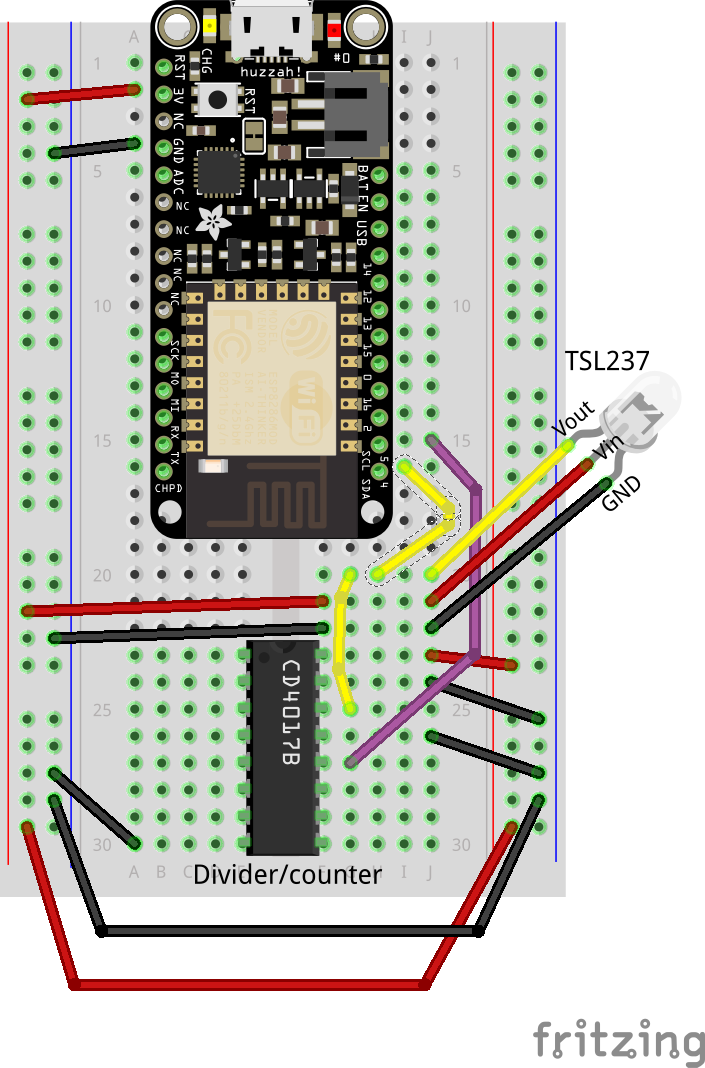
\includegraphics[width=\MFW]{Fritzing/feather_tsl237_bb.png}}{https://publicsensors.org/IntroSensors/Fritzing/feather_tsl237_bb.png}
		\caption[Complete light sensor circuit schematic]{An illustration of the circuit layout for sensing light coupling a \texttt{CD4017B} divider/counter with a \texttt{TSL237} Light-to-Frequency sensor. 
		Sub-circuit 2 is an addition to sub-circuit 1, which is not modified. 
		Wire colors retain the same meaning as in sub-circuit 1, with the additional purple wire representing divided frequency from the frequency-modulated sensor output.
		in which frequency is read directly from the sensor.}
		\labfig{feather_tsl237}
	\end{center}
\end{marginfigure}
The layout for adding sub-circuit 2 to your sensor assembly is shown in \reffig{feather_tsl237}.

\begin{enumerate}
	\item \textbf{Place your \texttt{CD4017B} on the breadboard.}
	
	The orientation of the \texttt{CD4017B} is indicated by the semi-circular indentation on one end.
	This is the upper end, which goes closest to the microcontroller.
	
	\item \textbf{Connect power and ground to the \texttt{CD4017B}.}
	
	The pins on the \texttt{CD4017B} are explained in the \htmladdnormallink{CD4017B datasheet} {https://www.ti.com/lit/ds/symlink/cd4017b.pdf}.
	The lower left pin is \texttt{GND}.
	The upper right pin is \texttt{Vin}, which in this case is connected via the power rail to \texttt{3.3 volts} from the microcontroller.
	
	\smallskip
	There are two additional ground connections. 
	\begin{itemize}
		\item[$\circ$] \textbf{Connect the \texttt{RESET} pin, immediately below \texttt{Vin}, to \texttt{GND}.} 
		\item[$\circ$] \textbf{Connect the \texttt{CLOCK INHIBIT} pin, two rows below the \texttt{RESET} pin, to \texttt{GND}.}	
	\end{itemize} 
	Both these pins modify the state of the \texttt{CD4017B} in ways that are not needed in our circuit.

	\item \textbf{Connect \texttt{Vout} from the \texttt{TSL237} to the \texttt{CLOCK} pin on the \texttt{CD4017B}.}

	The \texttt{CLOCK} pin is the input frequency signal for the \texttt{CD4017B}.
	Here, we connect it to \texttt{Vout} from the \texttt{TSL237}, which carries the voltage oscillating at the frequency to be divided. 
	
	\item \textbf{Connect \texttt{CARRY OUT} pin on the \texttt{CD4017B} to \texttt{Pin 5} on your \texttt{ESP8266}.}
	
	The \texttt{CARRY OUT} pin is the \texttt{CD4017B}'s output, which has $\frac{1}{10}$th the frequency of the \texttt{CLOCK} pin input. 

	\item \textbf{Test your frequency dividing circuit using the commands:}
\begin{lstlisting}[language=Python]
from frequency_median import median_of_n
from machine import Pin
p5 = Pin(5, Pin.IN)
timeout=300000
nrep=7
median_of_n(p5,nrep,timeout,verbose=True)
\end{lstlisting}	
	Most of this code is the same as in the sub-circuit 1 test.
	The only change is in pin number, from 4 to 5.
	The results will be something like
\begin{lstlisting}[language=Python]
536 [533, 533, 534, 536, 536, 537, 538]
(536, True)
\end{lstlisting}		
	\item \textbf{Repeat the assessment from \refsec{tsl237}, taking several measurements under different light conditions, calculating frequency from period, and critically assessing your observations.}

	What is the largest and smallest period and frequency you observe in the new tests?
	Do you see any evidence of changes in limits to the sensor's range, either at high or low light intensities, when the frequency signal is divided by the \texttt{CD4017B}?
	
\end{enumerate}

\loadMilestone{mlst:04g} % load milestone with tags id: mlst:04g


\subsection{Optimizing a light sensor driver}
With a working circuit that takes both direct and reduced frequency signals, you are now ready to code a driver to automatically select the best light measurement.



\subsubsection{\howto Code a ``driver'' for a \texttt{TSL237} light sensor}
\labsec{light_driv}



\begin{marginfigure}[-0cm]
	\begin{center}
		\htmladdnormallink{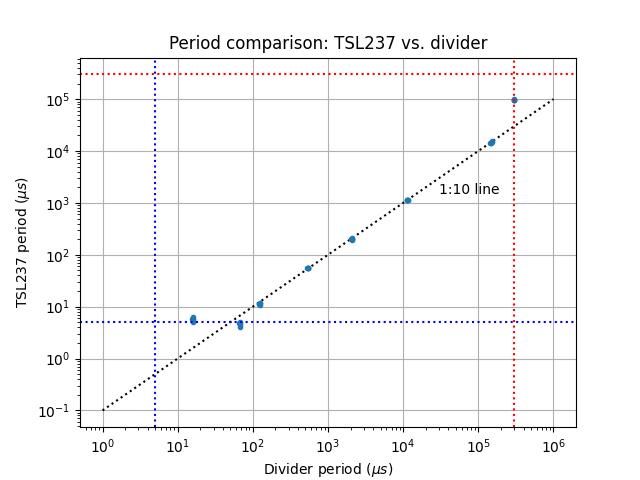
\includegraphics[width=\MFW]{Images/period_tsl237_divider.png}}{https://publicsensors.org/IntroSensors/Images/period_tsl237_divider.png}
		\caption[Periods from a light sensor and frequency divider]{Comparison of periods measured directly from a \texttt{TSL237} Light-to-Frequency sensor \textit{vs.} through a \texttt{CD4017B} counter/divider. 
		Note the \texttt{1:10} offsets in axis scales. 
		The solid line is the \texttt{1:10} line. 
		Because the divider reduces frequency 10-fold, the true ratio of periods (aside from signal noise) lies exactly on this line. 
		Deviations from the line indicate limits to one or both period measurements at high or low light levels.}
		\labfig{period_tsl237_divider}
	\end{center}
\end{marginfigure}

\reffig{period_tsl237_divider}


\vspace{4cm}

%https://www.amazon.com/gp/product/B01GMYPSWM/ref=ppx_od_dt_b_asin_title_s00?ie=UTF8&psc=1




\begin{itemize}
	\item  
\end{itemize}


\section{Environmental sensing with time: calibrate an acoustic distance sensor}
\labsec{cal_sonar}
\begin{itemize}
	\item  
\end{itemize}

\section{Environmental sensing with magnetism: measuring current and wind velocity}
\labsec{velocity}
\begin{itemize}
	\item  
\end{itemize}






%\loadMilestone{mlst:03a} % load milestone with tags id: mlst:02




\setchapterstyle{kao}
\setchapterpreamble[u]{\margintoc}
\chapter{Calibration, accuracy and precision of a thermistor-based heat sensor}
\labch{therm_calib}

Placeholder for thermistor calibration chapter.
\setchapterstyle{kao}
\setchapterpreamble[u]{\margintoc}
\chapter{Circuit design using Kirchhof's Laws}
\labch{circ_design}

Placeholder for circuit design chapter.

%\pagelayout{wide} % No margins
%\addpart{Digital interfaces for environmental analysis: Quantifying temperature, light and water chemistry}
%\pagelayout{margin} % Restore margins

\setchapterstyle{kao}
\setchapterpreamble[u]{\margintoc}
\chapter{Digital interfaces for environmental sensors}
\labch{digital_interfaces}

In \refch{circuits_intro}, we considered the fundamentals of constructing circuits that exploit the abilities of microcontrollers to measure voltage and time to quantify environmental variables.
These circuits were based on \textit{analog} sensors -- that is, sensors that return signals in the form of continuously variable voltages or time lags.
By integrating the microcontroller, circuit and analog sensor components, you assembled a device that provided a \textit{digital} signal -- a number that represents an observation of the corresponding environmental parameter.

A modern trend in sensor development is \textit{digital sensors}, whose output is intrinsically in the form of numbers rather than voltage or time.
If you used the external \DS3231 Real Time Clock in \refch{time_keeping}, you have already used a digital sensor.
In digital sensors, the circuitry and some of the microcontroller functions that you used to convert analog signals to digital outputs have been placed on the sensor itself.
This means that the user-designed circuitry and microcontroller interfaces can usually be greatly simplified compared to an analog sensor measuring the same quantity.

Because digital sensors typically return observations as numbers with many decimal places, it's tempting to overlook the fact that in many cases they may be less accurate and precise than analog sensors (or may cost more for comparable accuracy and precision).
It's important to keep in mind that digital sensors have the same basic operating principles and limitations as analog sensors.
The internal circuitry of digital sensors is designed by experts and mass-produced in sophisticated factories.
This means that the tradeoffs and optimizations in sensitivity, resolution, power consumption, \etc that you considered in working with analog sensors have been decided by highly skilled professionals.
Remember, though, that these circuits (and hence the digital sensors that use them) still have most of the same constraints you wrestled with in your own sensor design.

With those caveats in mind, digital sensors often have a number of advantages relative to analog sensors.
Depending on the type of digital sensor and the context, these advantages may include:
\begin{itemize}
	\item Digital sensors use digital \texttt{GPIO}s, which are more abundant than analog \texttt{GPIO}s on most microcontrollers;
	\item Protocols for communicating with digital sensors are two-way -- information such as settings, commands to take readings \etc can be sent to digital sensors to make them more efficient and versatile;
	\item Some digital sensor protocols support multiple sensors on one set of \texttt{GPIO}s and wires, with microcontrollers able to identify and query each of those sensors individually;
	\item Some digital protocols support very long wire connections (though others are limited to very short wires);
	\item Some digital sensors internally do complex computations, such as integrating angular orientation from angular accelerations, which would be expensive in terms of processor cycles and energy to perform on a microcontroller.
\end{itemize}
These advantages are evident in many industrial applications (cars, phones, \etc).
As a result, many useful digital environmental sensors are mass produced and amazingly cheap for their capabilities.

This chapter uses examples of readily available and scientifically informative environmental sensors to illustrate how to use several common communication protocols for digital sensors.
Many other examples using each of these protocols appear later in this book, in applications of data from digital sensors to drawing inferences and hypothesis testing about environmental mechanisms.
For some readers, one or two of these protocols may be sufficient for the examples and data collection applications at hand.
If so, it may be an efficient strategy to focus on that subset of protocols, returning to learn the others if and when the need arises.

\subsection{Communicating with digital sensors}
In practice, getting measurements from digital sensors usually involves two main elements: establishing the appropriate circuit connections, and finding (or, occasionally, writing) a \emph{driver}.
A driver is a piece of code that interfaces between a microcontroller and digital sensor.
The driver enables the user to interact with a digital sensor, \eg by setting measurement parameters or querying for data, with simple, intuitive high-level \Micropython commands.
The driver handles messages between the microcontroller and the digital sensor at a very low level, that takes some technical expertise and patience to understand.
Fortunately, \Micropython-based drivers are freely available online for many of the most useful digital environmental sensors, and more are being written all the time.
You typically don't need to know much about the inner workings of a driver to use it for obtaining environmental sensor readings.

Most digital sensors used in environmental sensing communicate using one of four protocols:

%\begin{itemize}
%	\item \textbf{Inter-Integrated Circuit (\i2c)}
%
%	The \htmladdnormallink{\i2c}{https://en.wikipedia.org/wiki/I\%C2\%B2C} protocol (pronounced ``eye squared sea'') is commonly used in digital sensors for time, light, accceleration, \etc, and is also used in many small TFT displays for microcontrollers.
%	%Adafruit provides a useful \htmladdnormallink{overview of \i2c}{https://learn.adafruit.com/adafruit-ft232h-with-spi-and-i2c-libraries/i2c-devices}.
%	\i2c is a ``2 wire'' protocol (in addition to \texttt{Vin} and \texttt{GND}).
%	\i2c is designed to work over relatively short distances ($\le$ a few meters), but \htmladdnormallink{\texttt{differential extenders}}{https://learn.sparkfun.com/tutorials/qwiic-differential-i2c-bus-extender-pca9615-hookup-guide/all} are available that greatly increase the distance over which \i2c devices can communicate.
%
%	\smallskip
%	\i2c supports multiple devices on one cable, but each device must have unique addresses.
%	Adafruit has written a useful \htmladdnormallink{summary of default \i2c addresses}{https://cdn-learn.adafruit.com/downloads/pdf/i2c-addresses.pdf}, describing addresses used by different types of sensors and other devices.
%	Because there are more types of devices than distinct addresses, there is overlap between the addresses of some different sensor types.
%	It's largely a matter of luck whether two sensor types have conflicting addresses, but works out most of the time.
%	Some \i2c devices have a mechanism, like movable jumpers, to change \i2c addresses so that two or more of these devices can co-exist on the same cable.
%
%	\item \textbf{1-Wire}
%
%	\htmladdnormallink{1-wire}{https://en.wikipedia.org/wiki/1-Wire} is a proprietary protocol design that, as the name implies, uses only one wire in addition to \texttt{Vin} and \texttt{GND}.
%	1-wire is used in relatively few sensor types, but is worth knowing about because one of those is an inexpensive and versatile \htmladdnormallink{temperature sensor}{https://datasheets.maximintegrated.com/en/ds/DS18B20.pdf} that is among the most useful available for environmental monitoring.
%
%	\smallskip
%	1-wire supports many (up to hundreds) of devices on a single cable, each of which can be independently queried for sensor readings because it has a unique ROM address.
%	1-wire supports lower (but still generally sufficient) data rates than \i2c, which (when properly configured) can operate over much longer cables.
%
%	\item \textbf{Universal Asynchronous Receiver-Transmitter (\uart)}
%
%	\htmladdnormallink{\uart}{https://en.wikipedia.org/wiki/Universal_asynchronous_receiver-transmitter} is a communications protocol with a long history of use in computer hardware (including communication between computers and microcontrollers), navigation equipment and many other industrial applications.
%	\uart supports communication between only two devices, and these devices must share common settings for a number of parameters. %(bit speed, character length, parity, and stop bits).
%	Common applications in environmental sensing include \texttt{GPS} receivers and Air Quality Index sensors.
%
%	\uart uses two wires (in addition to \texttt{Vin} and \texttt{GND}), one for transmitting and one for receiving.
%	In some applications (\eg, some \texttt{GPS} configurations) only one of these functions is utilized (\eg, transmit on the \texttt{GPS} and receive on the microcontroller) in which case only one of these wires is necessary.
%
%	\item \textbf{Serial Peripheral Interface (\spi)}
%
%	The \spi protocol is commonly used for some types of sensors, external radio communications, TFT displays, LED banks, \etc
%	\spi uses four wires (in addition to \texttt{Vin} and \texttt{GND}), three of which can be shared by multiple devices on the same cable but the fourth of which must be unique to each device.
%	Maximum data rates are higher than for \i2c devices.
%	Many digital sensors have both \spi and \i2c interfaces, so they can be used with either protocol.
%
%	%►Overview: https://learn.sparkfun.com/tutorials/serial-peripheral-interface-spi
%	%Technical info: https://en.wikipedia.org/wiki/Serial\_Peripheral\_Interface\_Bus
%	%Also see Adafruit tutorials on SPI sensors
%\end{itemize}

\begin{itemize}
	\item \textbf{Inter-Integrated Circuit (\i2c)}

	The \htmladdnormallink{\i2c}{https://en.wikipedia.org/wiki/I\%C2\%B2C} protocol (pronounced ``eye squared sea'') is commonly used in digital sensors for time, light, accceleration, \etc, and is also used in many small TFT displays for microcontrollers.

	\item \textbf{1-Wire}

	\htmladdnormallink{1-wire}{https://en.wikipedia.org/wiki/1-Wire}  is used in relatively few sensor types, but is worth knowing about because one of those is an inexpensive and versatile \htmladdnormallink{temperature sensor}{https://datasheets.maximintegrated.com/en/ds/DS18B20.pdf} that is among the most useful available for environmental monitoring.


	\item \textbf{Universal Asynchronous Receiver-Transmitter (\uart)}

	\htmladdnormallink{\uart}{https://en.wikipedia.org/wiki/Universal_asynchronous_receiver-transmitter} is a communications protocol with a long history of use in computer hardware, including communication between computers and microcontrollers.
	\uart is used in many Global Positioning System (GPS) receivers and Air Quality Index (AQI) sensors, in some Automatic Identification System (AIS) navigation equipment, and many other industrial applications.

	\item \textbf{Serial Peripheral Interface (\spi)}

	The \htmladdnormallink{\spi}{https://learn.sparkfun.com/tutorials/serial-peripheral-interface-spi} protocol is commonly used for some types of sensors, external radio communications, TFT displays, LED banks, \etc \spi interfaces are used on some microcontrollers to read from and write to microSD cards.
\end{itemize}



\section{ \i2c sensors }
\labsec{i2c_sensors}
\subsection{Background}
	%Adafruit provides a useful \htmladdnormallink{overview of \i2c}{https://learn.adafruit.com/adafruit-ft232h-with-spi-and-i2c-libraries/i2c-devices}.
\i2c is a ``2 wire'' protocol: it has two communications connections, \texttt{SDA} and \texttt{SCL}, in addition to \texttt{Vin} and \texttt{GND}.
Most microcontrollers have built-in hardware  \texttt{GPIO}s preconfigured as \texttt{SDA} and \texttt{SCL} for \i2c communications.
On most microcontrollers, it is also possible to use other \texttt{GPIO} pins for software-driven \i2c communications (``bit-banging''), often with somewhat reduced but perfectly adequate capabilities.
%This provides helpful flexibility when preconfigured \texttt{SDA} and \texttt{SCL} \texttt{GPIO}s are need for other uses, or when too many \i2c devices are needed .

\i2c is designed to work over relatively short distances ($\le$ a few meters), but \htmladdnormallink{\texttt{differential extenders}}{https://learn.sparkfun.com/tutorials/qwiic-differential-i2c-bus-extender-pca9615-hookup-guide/all} are available that greatly increase the distance over which \i2c devices can communicate.

A useful feature of \i2c is that it supports multiple devices on one cable (here, we're using ``cable'' as shorthand for the \i2c bus on the microcontroller, the wires connecting the microcontroller to the sensors, \etc).
However, there is a constraint: each device must have an address that is unique on any given cable.

Each type of \i2c-based digital sensor is typically pre-programmed with an address, associated with what kind of sensor it is.
This is very helpful for authors of \emph{drivers} (short codes designed to interface between a microcontroller and digital sensor).
However, it means that trying to use multiple sensors of the same type on a single \i2c cable often runs afoul of the unique address constraint.

Because there are more types of devices than distinct addresses, there are also overlaps between the addresses of some different sensor types.
Adafruit has written a useful \htmladdnormallink{summary of default \i2c addresses}{https://cdn-learn.adafruit.com/downloads/pdf/i2c-addresses.pdf}, describing addresses used by different types of sensors and other devices.


It's largely a matter of luck whether two sensor types have conflicting addresses, but works out most of the time.

For cases when it doesn't, some \i2c devices have a mechanism, like movable jumpers, to change \i2c addresses so that two or more of these devices can co-exist on the same cable.
Another alternative, of course, is to have more than one \i2c bus, \eg by having separate hardware and bit-banged \i2c buses.
Still another workaround is an \i2c \htmladdnormallink{multiplexer}{https://github.com/mcauser/micropython-tca9548a}, which is an \i2c device that can direct communications to any of eight \i2c devices attached to it (whether or  not they have the same addresses).
% The reference to the external RTC is \refsec{ext_i2c_time}

\subsection{ Measuring temperature with a high-resolution sensor }
As a first demonstration of sampling environmental conditions using the \i2c protocol, we will work with the \MCP9808 digital temperature sensor.
This is an inexpensive but high resolution sensor manufactured by Microchip Technology Inc., described in detail in the \htmladdnormallink{datasheet}{https://ww1.microchip.com/downloads/en/DeviceDoc/25095A.pdf}.
The basic sensor component is packaged onto a ``breakout board'' by a number of vendoers, including \htmladdnormallink{Adafruit}{https://www.adafruit.com/product/1782}.

The \MCP9808's temperature sensitivity is provided by a \htmladdnormallink{bandgap temperature sensor}{https://en.wikipedia.org/wiki/Silicon_bandgap_temperature_sensor}, whose output is relayed to an internal \adc before being passed to the \i2c interface.
This progression, which is typical of digital environmental sensors, closely reflects the fundamental similarity between the signal processing steps you used in \refsec{cal_therm} to obtain numerical output from an analog thermistor signal.
However, in the digital sensor, the steps you performed on the microcontroller (analog to digital conversion, calculation of temperature from voltage using a calibration) are instead performed inside the sensor.

As shown in Table 5-2 and Figure 2-12 in the datasheet, the \MCP9808 can be set to take very high resolution temperature measurements at a relatively slow rate ($\pm 0.0625^\circ$ \texttt{C} at 4 \gls{spsLabel}), or lower resolution measurements at faster rates (\eg,$\pm 0.5 ^\circ$ \texttt{C} at 33 \gls{spsLabel}).
In this and the next sections, accuracy and precision are higher priorities than high sampling rates.
We will therefore use \i2c to command the sensor to use the slowest, highest resolution sampling rates.

\subsubsection{\howto Set up an \MCP9808 temperature sensor}

\begin{marginfigure}
	\begin{center}
		\htmladdnormallink{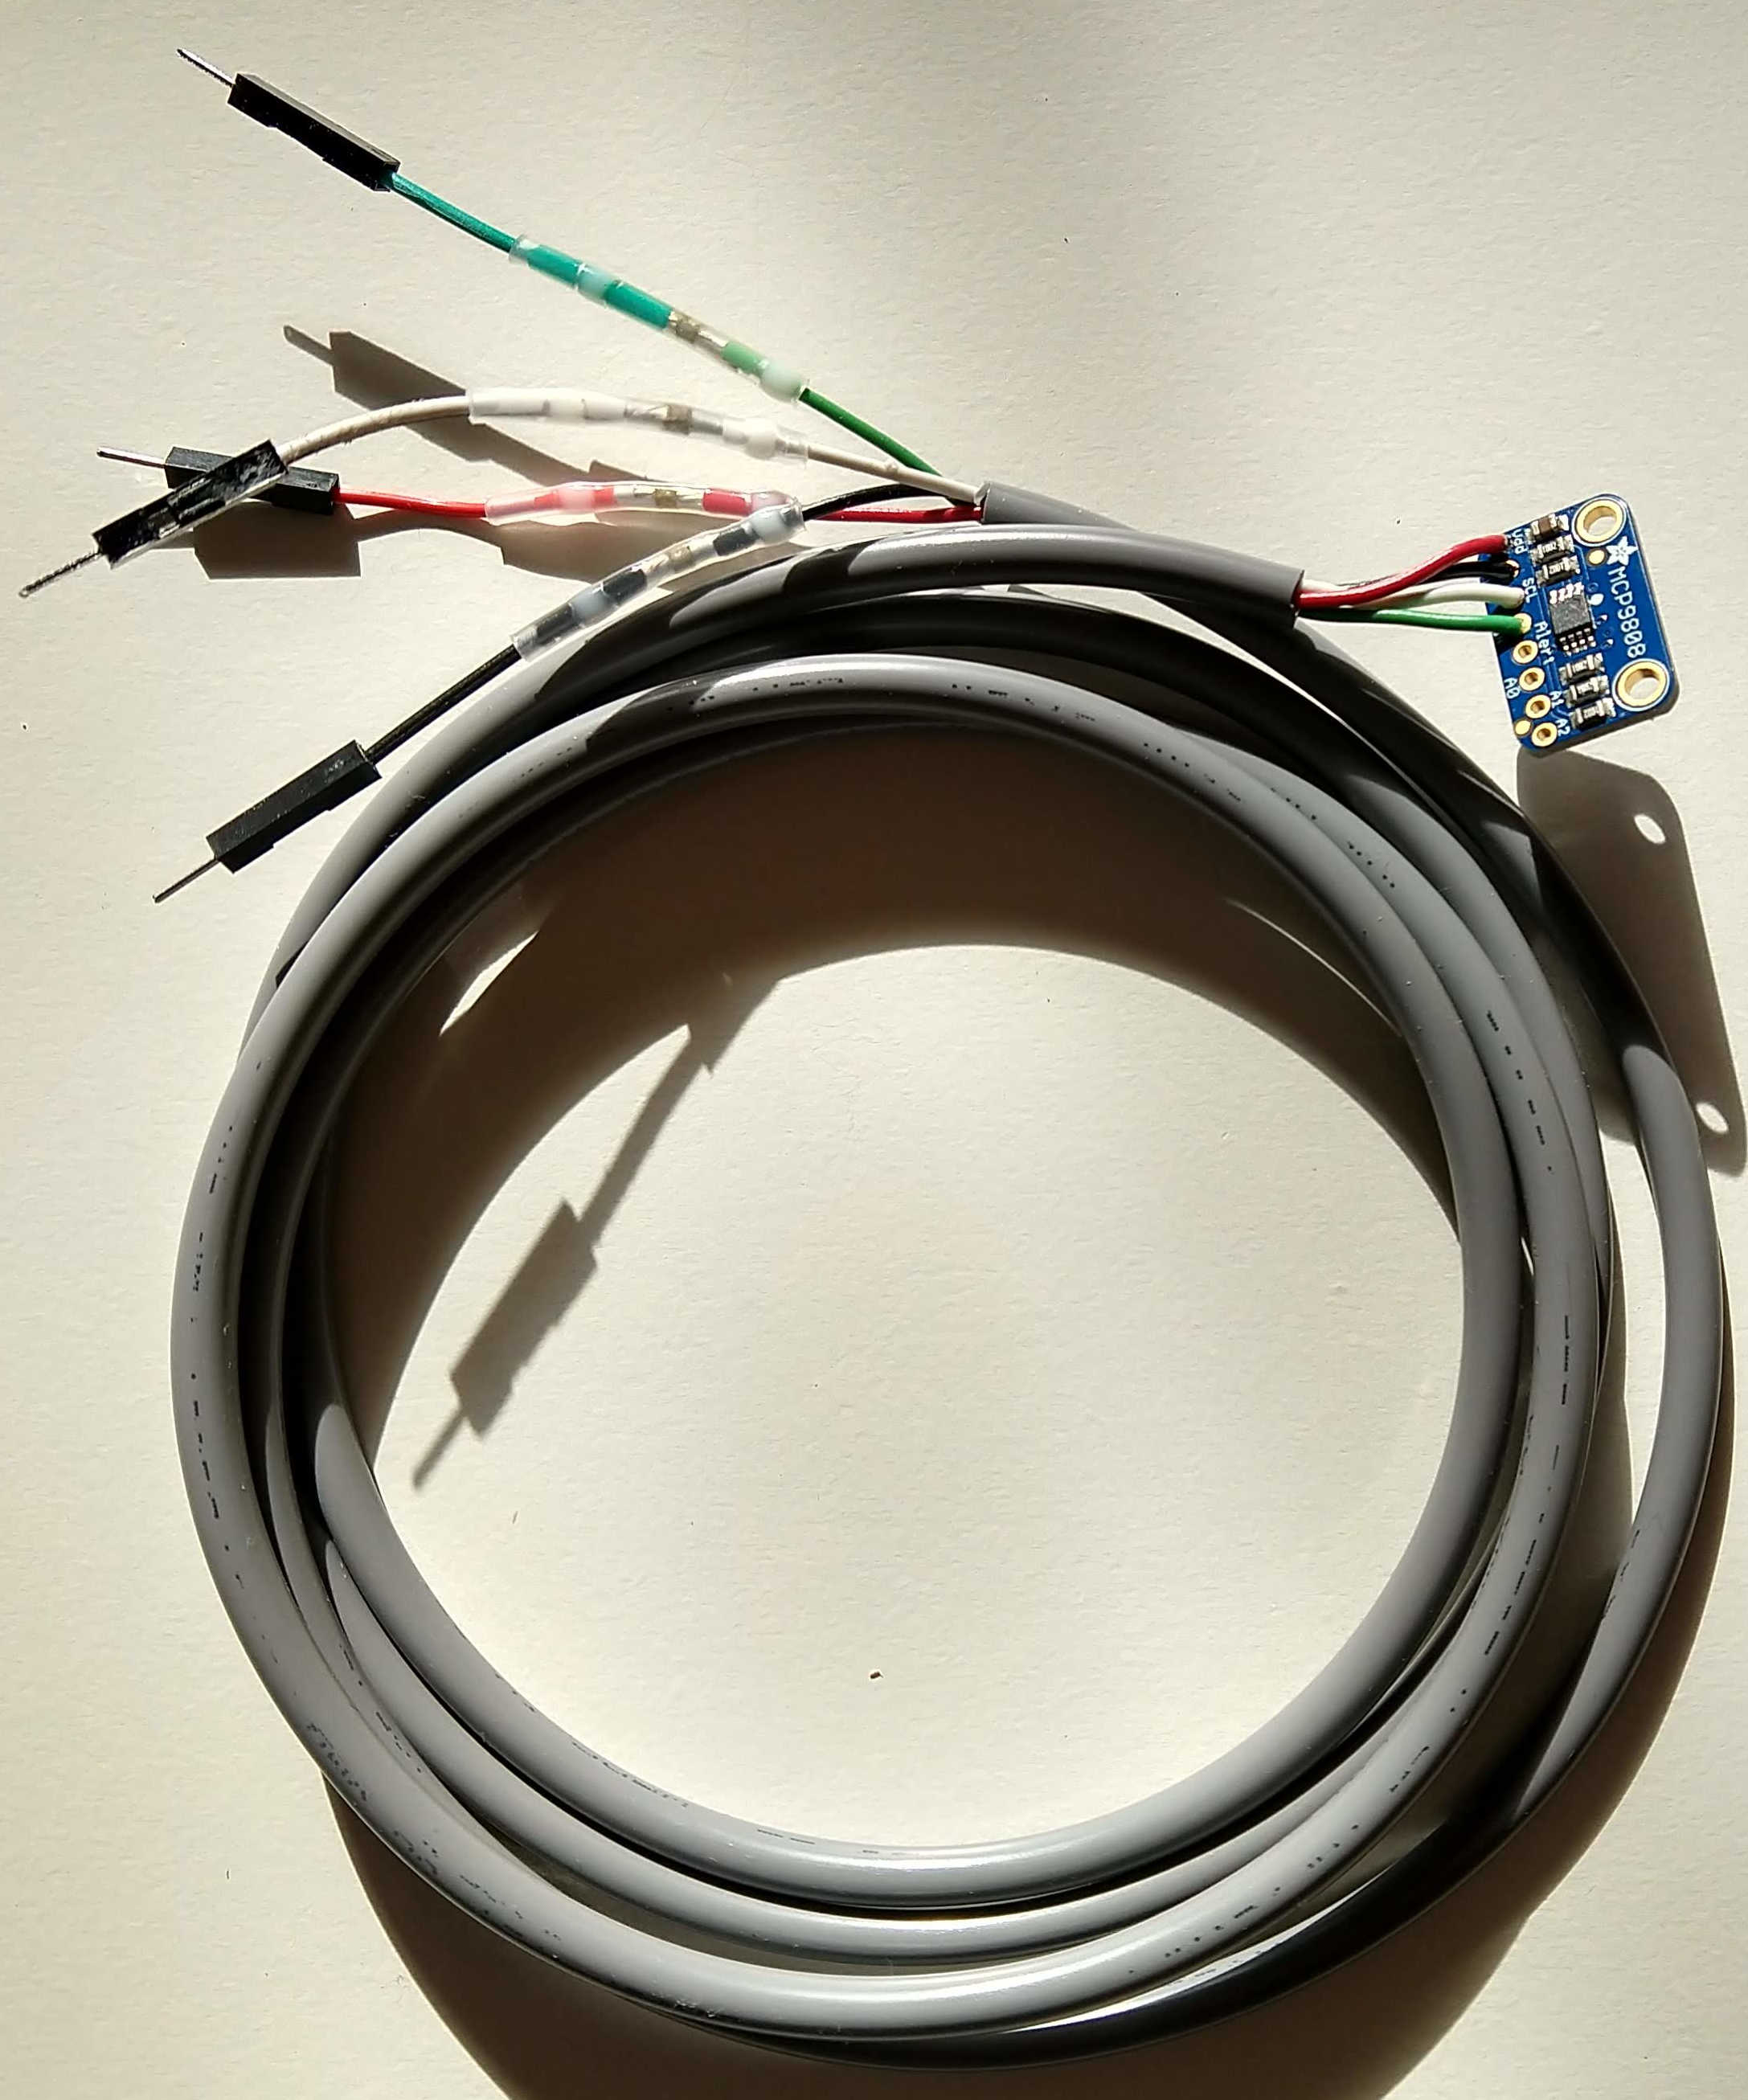
\includegraphics[width=\MFW]{Images/MCP9808_on_cable_cropped.jpg}}{https://github.com/publicsensors/IntroSensors/blob/digital/Images/MCP9808_on_cable_cropped.jpg}
		%\includegraphics[height=5cm]{Images/DS3231breadboard.jpg}
		\caption[MCP9808 on breadboard]{An \MCP9808 temperature sensor soldered onto a cable with 4 conductors (red $\leftrightarrow$ \texttt{Vdd}, black $\leftrightarrow$ \texttt{GND}, white $\leftrightarrow$ \texttt{SCL} and green $\leftrightarrow$ \texttt{SDA}).
		Male jumper ends are connected to the other end of the cable with \glspl{ssw_connector}.
		Note that, for clarity, the jumpers on the other end of the cable have colors consistent with the corresponding wires attached to the sensor.}
		\labfig{mcp9808_cable}
	\end{center}
\end{marginfigure}


\begin{marginfigure}
	\begin{center}
		\htmladdnormallink{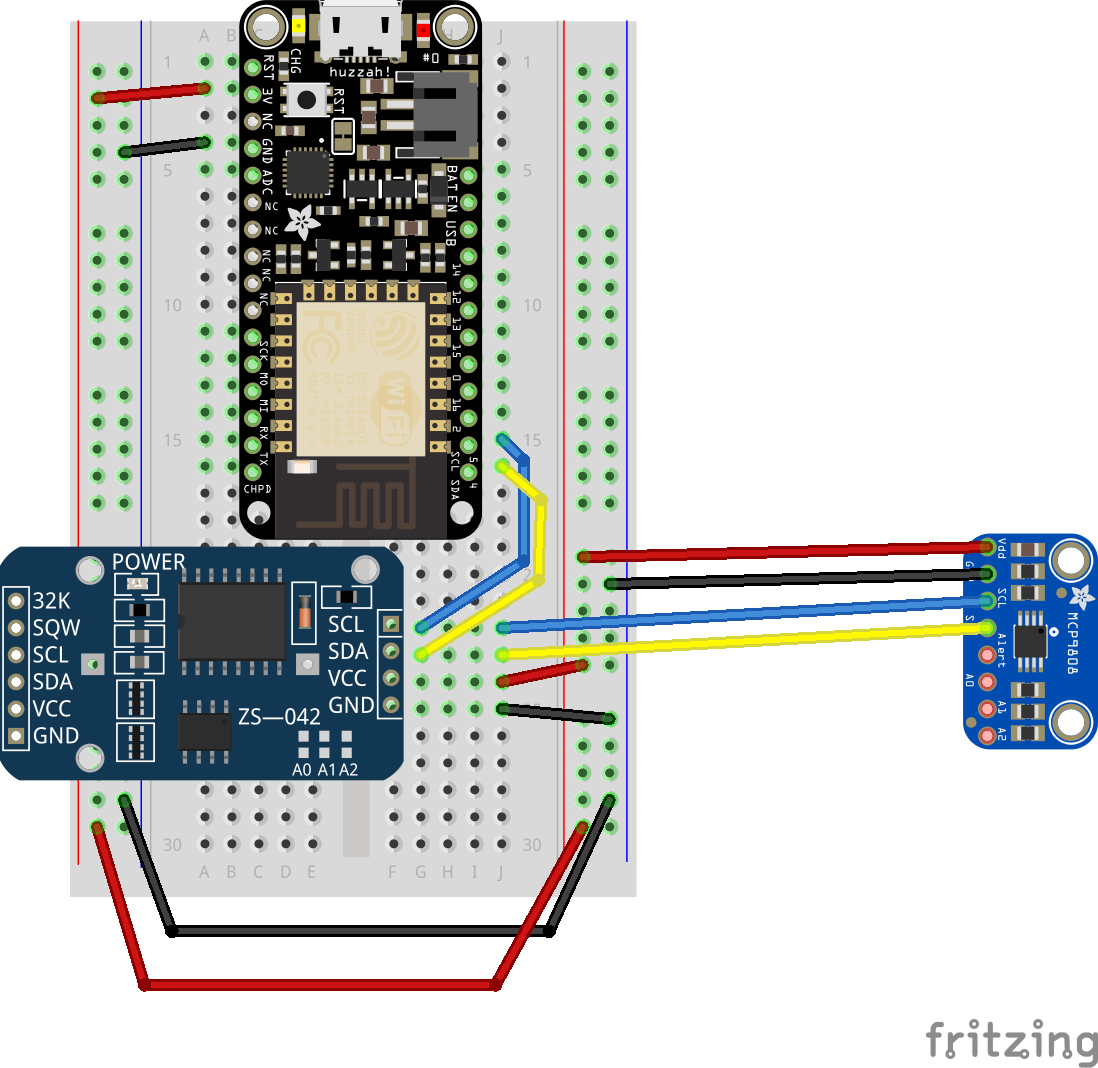
\includegraphics[width=\MFW]{Fritzing/feather_MCP9808_bb.png}}{https://github.com/publicsensors/IntroSensors/blob/digital/Fritzing/feather_MCP9808_bb.png}
		%\includegraphics[height=5cm]{Images/DS3231breadboard.jpg}
		\caption[MCP9808 on breadboard]{An example of layout and wire connections for the \MCP9808 temperature sensor and ESP8266 microcontroller. The circuit layout is similar to that used for the DS3231 external Real Time Clock. The DS3231 is left in the figure to emphasize that \i2c can support multiple devices simultaneously, but this exercise works equally well with or without the DS3231.}
		\labfig{mcp9808_breadboard}
	\end{center}
\end{marginfigure}


\begin{enumerate}
	\item \textbf{Connect wires to the GND, Vdd, SCL and SDA pins on the \MCP9808}.

	Like in the thermistor calibration in \refsec{cal_therm}, we will use ``water baths'' made of paper cups to expose the \MCP9808 sensors to known temperatures without getting them wet.
	This is most easily done if the sensor is connected to the microcontroller by extra long wires.

	\smallskip
	If your \MCP9808 has pins soldered to it, you can use two or more jumpers attached in series to give enough scope to move the sensor around.
	If your sensor does not have pins, you can solder some on, or alternatively solder long wires directly to the sensor (\reffig{mcp9808_cable}).

	You can then connect the other ends of the wires to the breadboard by soldering pins or male jumpers onto them; \reffig{mcp9808_cable} shows an example of this.
	The cable in this figure was made with \glspl{ssw_connector}, a fast and convenient way to join and protect two wire ends.

	Alternatively, you can attach wires directly to terminals (\eg, like \htmladdnormallink{these}{https://www.adafruit.com/product/2137?gclid=CjwKCAjwq9mLBhB2EiwAuYdMtZGP6ggrSAALQm8J7sbJ8Mwr6zWCWucqFVLvuSnaAGO22bPzFGNxmhoCVvEQAvD_BwE}), that then insert into breadboards.


	\item \textbf{Connect the GND and 3V pins on the ESP8266 to the GND and Vdd pins on the \MCP9808}.

	The circuit layout for the \MCP9808 is shown in \reffig{mcp9808_breadboard}.


	\item Connect the \texttt{SDA} (\#4) pin on the ESP8266 to the \texttt{SDA} pin on the \MCP9808, and the  \texttt{SCL} (\#5) pin on the ESP8266 to \texttt{SCL} on the \MCP9808.
	\item \textbf{Download the driver module provided on github by \texttt{@kfricke} called \htmladdnormallink{mcp9808.py}{https://raw.githubusercontent.com/kfricke/micropython-mcp9808/master/mcp9808.py} for the \MCP9808 temperature sensor.}

	Save it into a \texttt{Codes} directory on your computer.

	\item \textbf{Copy } \lstinline{mcp9808.py} \textbf{onto your microcontroller, using \thonny, \texttt{WebREPL} or \mpfshell (see the methods from \refch{connect} if you have questions).}
	\item %You are now ready to test your \DS3231 \rtc.
	\textbf{Set up the \i2c connection to your \MCP9808:}
\begin{lstlisting}[language=Python]
from machine import I2C, Pin
import mcp9808

i2c=I2C(scl=Pin(5),sda=Pin(4))
temp_mcp9808=mcp9808.MCP9808(i2c=i2c)
\end{lstlisting}
	\item \textbf{Set the resolution on your \MCP9808 to the highest possible}, with:
\begin{lstlisting}[language=Python]
temp_mcp9808.set_resolution(mcp9808.TEMP_RESOLUTION_MAX)
\end{lstlisting}

	\item \textbf{Query the temperature from your \MCP9808}:

	Here, there are two choices:
	If your microcontroller can do floating point math, use
\begin{lstlisting}[language=Python]
temp_mcp9808.get_temp()
\end{lstlisting}
The result of this command is the temperature in degrees Celsius, expressed as a floating point number.

\smallskip
If your microcontroller cannot do floating point math, use
\begin{lstlisting}[language=Python]
temp_mcp9808.get_temp_int()
\end{lstlisting}
The result of this command is two numbers.
The first is the temperature in whole degrees Celsius, expressed as an integer.
The second is the remaining fraction of a degrees Celsius, expressed as another integer.

\end{enumerate}
\loadMilestone{mlst:05a} % load milestone with tags id: mlst:04c


\subsection{\color{gray} Multiple sensors on a device: Temperature and pressure on an MS5803 \color{black}}
\subsection{\color{gray} Using I2C over long cables with differential extenders \color{black}}


\section{\color{gray}1-wire sensors \color{black}}
\labsec{1wire_sensors}
\subsection{\color{gray} Background \color{black}}
1-wire is a proprietary protocol design that, as the name implies, uses only one wire in addition to \texttt{Vin} and \texttt{GND}.
1-wire is used in relatively few sensor types, but is worth knowing about because one of those is an inexpensive and versatile \htmladdnormallink{temperature sensor}{https://datasheets.maximintegrated.com/en/ds/DS18B20.pdf} that is among the most useful available for environmental monitoring.

\smallskip
1-wire supports many (up to hundreds) of devices on a single cable, each of which can be independently queried for sensor readings because it has a unique ROM address.
1-wire supports lower (but still generally sufficient) data rates than \i2c, which (when properly configured) can operate over much longer cables.

\subsection{\color{gray} Temperature measurements with DS18B20 digital sensors \color{black}}
\subsection{\color{gray} Accuracy and precision of DS18B20 temperature sensors \color{black}}
\subsubsection{\color{gray} Improve the accuracy and precision of DS18B20 temperature measurements with recalibration \color{black}}
\subsubsection{\color{gray} Monitoring temperature changes across time \color{black}}


\section{\color{gray}\uart sensors \color{black}}
\labsec{UART_sensors}
\subsection{\color{gray} Background \color{black}}
	\uart supports communication between only two devices, and these devices must share common settings for a number of parameters. %(bit speed, character length, parity, and stop bits).
Common applications in environmental sensing include \texttt{GPS} receivers and Air Quality Index sensors.

\uart uses two wires (in addition to \texttt{Vin} and \texttt{GND}), one for transmitting and one for receiving.
In some applications (\eg, some \texttt{GPS} configurations) only one of these functions is utilized (\eg, transmit on the \texttt{GPS} and receive on the microcontroller) in which case only one of these wires is necessary.
\subsection{\color{gray} Measuring position and velocity using the Global Positioning System (GPS) \color{black}}

\section{\color{gray}\spi sensors \color{black}}
\labsec{spi_sensors}
\subsection{\color{gray} Background \color{black}}
	Additional details about \spi are provided by \htmladdnormallink{WikiPedia}{https://en.wikipedia.org/wiki/Serial\_Peripheral\_Interface\_Bus} uses four wires (in addition to \texttt{Vin} and \texttt{GND}), three of which can be shared by multiple devices on the same cable but the fourth of which must be unique to each device.
Maximum data rates are higher than for \i2c devices.
Some digital sensors have both \spi and \i2c interfaces, so they can be used with either protocol.
\subsection{\color{gray} SPI control of a TFT display panel \color{black}}


%
% \vspace{10cm}
%
%
% \section{Construction, calibration and use of a colorometric pH sensor}
% \labsec{pH_sensor}
% Placeholder for pH sensor section.

\setchapterstyle{kao}
\setchapterpreamble[u]{\margintoc}
\chapter{Data telemetry and protocols for sensor communications}
\labch{telem_sens_coms}

Placeholder for data telemetry and sensor communications chapter.

\pagelayout{wide} % No margins
\addpart{Practical skills in environmental sensing}
\pagelayout{margin} % Restore margins
\setchapterstyle{kao}
\setchapterpreamble[u]{\margintoc}
\chapter{\color{gray} Computer Aided Design (CAD) and fabrication \color{black}}
\labch{CAD_fab}

Placeholder for CAD/fabrication chapter.

\setchapterstyle{kao}
\setchapterpreamble[u]{\margintoc}
\chapter{\color{gray} Design of printed circuit boards \color{black}}
\labch{PCB_design}

Placeholder for PCB design chapter.
s \setchapterstyle{kao}
\setchapterpreamble[u]{\margintoc}
\chapter{Inference of mechanisms and processes from environmental sensor data}
\labch{inferences}

Placeholder for inferences from data chapter.


%\pagelayout{wide} % No margins
%\addpart{Sound and water waves}
%\pagelayout{margin} % Restore margins
%
%\setchapterstyle{kao}
\setchapterpreamble[u]{\margintoc}
\chapter{Time/space resolution of wave trains using wave height and bottom pressure}
\labch{waves}

Placeholder for wave train chapter.

%\setchapterstyle{kao}
\setchapterpreamble[u]{\margintoc}
\chapter{Assembling a sonar circuit: calibrating the speed of sound in air and water}
\labch{speed_sound}

Placeholder for speed of sound chapter.

%\pagelayout{wide} % No margins
%\addpart{Inference of mechanisms and processes from environmental sensor data}
%\pagelayout{margin} % Restore margins
%
%\setchapterstyle{kao}
\setchapterpreamble[u]{\margintoc}
\chapter{Inference of mechanisms and processes from environmental sensor data}
\labch{inferences}

Placeholder for inferences from data chapter.

%\setchapterstyle{kao}
\setchapterpreamble[u]{\margintoc}
\chapter{Vertical structure in lab and field water columns}
\labch{water_cols}

Placeholder for water column analysis chapter.

%%%\chapter{Vertical structure in lab and field water columns}
%%
%\pagelayout{wide} % No margins
%\addpart{Quantifying position, orientation and movement}
%\pagelayout{margin} % Restore margins

\appendix % From here onwards, chapters are numbered with letters, as is the appendix convention

%Original: \chaptername
%\providecommand*{\chaptername}{}
%\renewcommand*{\chaptername}{Appendix}
%After renewal: \chaptername

\pagelayout{wide} % No margins
\addpart{Appendix}
\labpart{conns}
\pagelayout{margin} % Restore margins

%Milestone file: Milestones.tex
\setchapterstyle{kao}
\setchapterpreamble[u]{\margintoc}
\chapter{Milestones}
\labch{milestones}
 
% Create a counter for Milestones
% Note this is redefined and reset in the Milestones chapter
% to give appropriate numbering
%\newcounter{mscntr}[section]
\renewcommand{\themscntr}{\arabic{section}.\arabic{mscntr}}
% A command to increment and print the milestone number, with
% smart handling of the following space.
%\newcommand{\showmscntr}{\stepcounter{mscntr}\themscntr\xspace}

%<*mlst:ov>
\begin{kaobox}[backgroundcolor=\MScolor,frametitlebackgroundcolor=\MScolor,frametitle=Milestones Overview]
%	\begin{itemize}
%		\item	
		Milestones enable you to demonstrate key practical skills, and enable your instructor to give you credit for your hands-on work with microcontrollers, circuits, environmental housings, \etc \,
		Milestones also indicate \emph{to you} that you have successfully mastered an important step in environmental instrument building. \,
		Finally, the work you do in Milestones records many useful commands and sensor-building methods, so that they are easy to find when needed later on.\,
		A full list of Milestones is given in Appendix \ref{ch:milestones}.
%	\end{itemize}
\end{kaobox}
%</mlst:ov>

\section{\refch{connect} Milestones}
\setcounter{mscntr}{0}
%<*mlst:01>
\begin{kaobox}[backgroundcolor=\MScolor,frametitlebackgroundcolor=\MScolor,frametitle= \showmscntr Milestone: Connecting to REPL via USB]
\begin{itemize}
	\item [$\Box$] This Milestone is to communicate with your microcontroller via USB. \,
	The specific goal is to demonstrate to an instructor that you have connected to a REPL session on your microcontroller, and obtained the $~>>>$ Python prompt. \, 
	When you obtain this prompt, complete the assignment by uploading a screenshot of your \texttt{mpfshell} or BeagleTerm REPL session. 
\end{itemize}
\end{kaobox}
%</mlst:01>

%<*mlst:01a>
\begin{kaobox}[backgroundcolor=\MScolor,frametitlebackgroundcolor=\MScolor,frametitle=\showmscntr Milestone: Activating WiFi on your microcontroller]
	\begin{itemize}
		\item [$\Box$] This Milestone is to activate both WiFi modes on your microcontroller.\space 
		The specific goals are to demonstrate: (a) setting up and activating an Access Point (AP), with your own \emph{informative} SSID and password; and, (b) connecting your microcontroller in Station (STA) mode to a router so that it can communicate via the Internet. \,
		After you activate both modes, complete the assignment by uploading a screenshot of your \texttt{mpfshell} or BeagleTerm REPL session showing the commands and output.
	\end{itemize}
\end{kaobox}
%</mlst:01a>

%<*mlst:01b>
\begin{kaobox}[backgroundcolor=\MScolor,frametitlebackgroundcolor=\MScolor,frametitle=\showmscntr Milestone: Connecting to REPL via WiFi]
	\begin{itemize}
		\item[$\Box$] This Milestone is to communicate with your microcontroller via WiFi. \,
		The specific goals are to demonstrate to an instructor that you have (a) connected to a REPL session on your microcontroller, and (b) uploaded and downloaded a file over WiFi using either \texttt{WebREPL} or \mpfshell.
		\begin{itemize}
			\item[$\Box$] Create a plain text file called ``\lstinline{main.py}'', containing the three lines:  \\
			
\lstinline{print('Launching main.py...')} \\

\lstinline{import esp}  \\

\lstinline{esp.osdebug(None)}

		\item[$\Box$] Upload this file onto your microcontroller over WiFi.
		\item[$\Box$] Enter a \texttt{REPL} session and reboot with \texttt{<ctrl>-d}.
		\item[$\Box$] Verify that the message ``Launching main.py'' is output, confirming this script was executed.
		\item[$\Box$] Download \lstinline{main.py} back onto your computer over WiFi, saving it under a different name.
	\end{itemize} 
	In Micropython, a file named \lstinline{main.py} is automatically executed (if it exists) when your microcontroller boots up. \,
	This example serves a useful purpose, which is to suppress unwanted debugging messages, which can be distracting when working with your microcontroller. \\

	When you have performed these tasks, complete the assignment by uploading a screenshot of your \texttt{mpfshell} or \texttt{WebREPL} session.
	\end{itemize}
\end{kaobox}
%</mlst:01b>

%<*mlst:01c>
\begin{kaobox}[backgroundcolor=\MScolor,frametitlebackgroundcolor=\MScolor,frametitle=\showmscntr Milestone: Generating random strings]
	\begin{itemize}
		\item [$\Box$] This Milestone is to write a Python function that generates random strings from a set of characters that you supply (defaulting to the set of upper and lower case characters in the English alphabet). \,
		Compose this function in an editor on your computer, and use \texttt{webREPL} or \texttt{mpfshell} to upload it to your microcontroller. \,
		The syntax of a Python function is illustrated in the \texttt{randint} example. 
		\begin{itemize}
			\item[$\Box$] The first line is a \texttt{definition} statement, e.g. \lstinline{def randstr(str_len, char_list=['a','b','c','d','e','f','g','h','i','j','k','l','m','n','o','p','q','r','s','t','u','v','w','x','y','z']):}
			\item[$\Box$] The body of the function is an adaptation of the commands you used to generate random strings in the REPL session.
			\item[$\Box$] The final line is a \texttt{return} statement, e.g. \lstinline{return rnd_str}, specifying exactly what output the function has.
			\item[$\Box$] Remember to observe the indentation requirements of Python for the statements inside the function.
		\end{itemize}
		After you write, test and debug your function, complete the assignment by uploading your code and a screenshot of your \texttt{mpfshell} or BeagleTerm REPL session showing the function importation and output.
	\end{itemize}
\end{kaobox}
%</mlst:01c>



\section{\refch{first_exercises} Milestones}
\setcounter{mscntr}{0}
%<*mlst:02a>
%\begin{kaobox}[frametitle=Milestone]
%	\begin{itemize}
%		\item \loadMilestone{mlst:02} % load milestone with tags id: mlst:02
%	\end{itemize}
%\end{kaobox}

%\section{Milestone}
%\begin{itemize}
%	\item [$\Box$] %\textbf{Using GPIOs as outputs}
%
%	Demonstrate to an instructor the Python commands to turn on and off the blue LED connected to GPIO 2.
%\end{itemize}
\begin{kaobox}[backgroundcolor=\MScolor,frametitlebackgroundcolor=\MScolor,frametitle=\showmscntr Milestone: Using GPIOs as outputs]
%\begin{kaobox}[backgroundcolor=BurntOrange,frametitlebackgroundcolor=BurntOrange,frametitle=Using GPIOs as outputs]
\begin{itemize}
	\item [$\Box$] %\textbf{Using GPIOs as outputs}
	
	Demonstrate to an instructor the Python commands to create an informatively named Pin object connected to GPIO 2 in output mode, and use it to turn on and off the blue LED.
	Then, complete the assignment by uploading a screenshot of your \texttt{mpfshell} or \texttt{WebREPL} session.
\end{itemize}
\end{kaobox}
%</mlst:02a>

%<*mlst:02b>
\begin{kaobox}[backgroundcolor=\MScolor,frametitlebackgroundcolor=\MScolor,frametitle=\showmscntr Milestone: Connecting power and ground rails on a breadboard]
	%\begin{kaobox}[backgroundcolor=BurntOrange,frametitlebackgroundcolor=BurntOrange,frametitle=Using GPIOs as outputs]
	\begin{itemize}
		\item [$\Box$] %\textbf{Using GPIOs as outputs}
		
		Demonstrate to an instructor a correctly wired breadboard, in which: \,
		Both negative rails are connected to the microcontroller's \texttt{GND} pin; and, both positive rails are connected to the \texttt{3V} pin. \,
		Use a multimeter to show that all the rails are properly connected.
		\, Then, complete the assignment by uploading a photograph or sketch of your circuit.
	\end{itemize}
\end{kaobox}
%</mlst:02b>

%<*mlst:02c>
\begin{kaobox}[backgroundcolor=\MScolor,frametitlebackgroundcolor=\MScolor,frametitle=\showmscntr Milestone: Controlling an input \texttt{GPIO} with a button]
	%\begin{kaobox}[backgroundcolor=BurntOrange,frametitlebackgroundcolor=BurntOrange,frametitle=Using GPIOs as outputs]
	\begin{itemize}
		\item [$\Box$] %\textbf{Using GPIOs as outputs}
		
		Demonstrate to an instructor a correctly wired circuit, in which a momentary button drives \texttt{GPIO 2}.
		Show that:
		\begin{itemize}
			\item[$\circ$] When the button is depressed, \texttt{GPIO 2} has value \texttt{0}.
			\item[$\circ$] When the button is released, \texttt{GPIO 2} has value \texttt{1}.
			\item[$\circ$] The blue LED correctly indicates button position.
		\end{itemize}
		\, Then, complete the assignment by uploading a photograph or sketch of your circuit.
	\end{itemize}
\end{kaobox}
%</mlst:02c>

%<*mlst:02d>
\begin{kaobox}[backgroundcolor=\MScolor,frametitlebackgroundcolor=\MScolor,frametitle=\showmscntr Milestone: Setting up an \texttt{interrupt} to respond to button presses]
	%\begin{kaobox}[backgroundcolor=BurntOrange,frametitlebackgroundcolor=BurntOrange,frametitle=Using GPIOs as outputs]
	\begin{itemize}
		\item [$\Box$] %\textbf{Using GPIOs as outputs}
		
		Demonstrate to an instructor the interrupt created by the python script \lstinline{button_interrupt.py}. \,
		Show that button presses trigger the \texttt{GPIO 2}interrupt, and result in toggling the red LED attached to \texttt{GPIO 0}.
		\, Then, complete the assignment by uploading a screenshot or copy of your \texttt{REPL} session showing the correct output responses to button presses.
	\end{itemize}
\end{kaobox}
%</mlst:02d>

%<*mlst:02e>
\begin{kaobox}[backgroundcolor=\MScolor,frametitlebackgroundcolor=\MScolor,frametitle=\showmscntr Milestone: Powering an external LED]
	%\begin{kaobox}[backgroundcolor=BurntOrange,frametitlebackgroundcolor=BurntOrange,frametitle=Using GPIOs as outputs]
	\begin{itemize}
		\item [$\Box$] %\textbf{Using GPIOs as outputs}
		
		Demonstrate to an instructor a correctly wired circuit to power an external LED.
		\, Then, complete the assignment by uploading a photograph or sketch of your circuit.
	\end{itemize}
\end{kaobox}
%</mlst:02e>

%<*mlst:02f>
\begin{kaobox}[backgroundcolor=\MScolor,frametitlebackgroundcolor=\MScolor,frametitle=\showmscntr Milestone: Using a relay to control an LED]
	%\begin{kaobox}[backgroundcolor=BurntOrange,frametitlebackgroundcolor=BurntOrange,frametitle=Using GPIOs as outputs]
	\begin{itemize}
		\item [$\Box$] %\textbf{Using GPIOs as outputs}
		
		Demonstrate to an instructor a correctly wired circuit to switch power on and off to an external LED.
		\, Then, complete the assignment by uploading a photograph or sketch of your circuit.
	\end{itemize}
\end{kaobox}
%</mlst:02f>


%<*mlst:02>
\begin{kaobox}[backgroundcolor=\MScolor,frametitlebackgroundcolor=\MScolor,frametitle=\showmscntr Milestone: Snoozing an LED using PWM]
\begin{itemize}
	\item [$\Box$] This Milestone is to complete the circuits described in \refch{first_exercises}. \,
	
	The specific goal is to demonstrate to an instructor the working circuit, with a ``snoozing'' LED driven by 3.3 \texttt{volt} power from the microcontroller's \texttt{3V} pin and regulated by Pulsed Width Modulation (PWM). \,
	
	When you demonstrate the circuit, complete the assignment by uploading a photograph or sketch of your breadboard layout.
\end{itemize}
\end{kaobox}
%</mlst:02>

\section{\refch{time_keeping} Milestones}
\setcounter{mscntr}{0}
%<*mlst:03>
\begin{kaobox}[backgroundcolor=\MScolor,frametitlebackgroundcolor=\MScolor,frametitle=\showmscntr Milestone: Setting Real Time Clocks using the Network Time Protocol]
	\begin{itemize}
		\item [$\Box$] This Milestone is to demonstrate use of the onboard and external \texttt{RTC}s. \,
		
		The specific goal is to use your ESP8266's \texttt{WiFi} connection to your classroom or home router to: (a) obtain the current time from a \texttt{NTP} server, and (b) set both the on-board and \texttt{DS3231} \texttt{RTC}s to correct time. \,
		
		When you have set your \texttt{RTC}s, complete the assignment by uploading a screenshot or transcript of your REPL session.
	\end{itemize}
\end{kaobox}
%</mlst:03>

%<*mlst:03a>
\begin{kaobox}[backgroundcolor=\MScolor,frametitlebackgroundcolor=\MScolor,frametitle=\showmscntr Milestone: Generating a detaset of time-keeping errors]
	\begin{itemize}
		\item [$\Box$] This Milestone is to generate a dataset using the \lstinline{time_compare} script. \,
		
		The specific goal is to agree with your peers on time sampling parameters, and to collect a full dataset using your microcontroller/\rtc combination.  \,
		
		When your sampling runs are finished, complete the assignment by uploading your data files so that they may be collected and shared with others in your class for a comparative statistical analysis in the next section.
	\end{itemize}
\end{kaobox}
%</mlst:03a>

%<*mlst:03a>
\begin{kaobox}[backgroundcolor=\MScolor,frametitlebackgroundcolor=\MScolor,frametitle=\showmscntr Milestone: Initial plotting of time-keeping errors]
	\begin{itemize}
		\item [$\Box$] This Milestone is to plot the time-keeping error dataset using the \lstinline{lineplot_TC_data} script. \,
		
		Use this script to visualize the magnitude and direction of errors, represented by differences between elapsed time measured using the onboard \rtc, the xternal \rtc and \ntp.
		Demonstrate using the interactive navigation widgets to zoom into specific parts of the dataset.  \,
		
		When you have successfully plotted the datset, complete the assignment by saving and uploading a \texttt{png} or \texttt{jpg} image of your plots.
	\end{itemize}
\end{kaobox}
%</mlst:03a>

%<*mlst:03b>
\begin{kaobox}[backgroundcolor=\MScolor,frametitlebackgroundcolor=\MScolor,frametitle=\showmscntr Milestone: Visualizing your devices' \textit{vs.} the population's time-keeping errors]
	\begin{itemize}
		\item [$\Box$] This Milestone is to replot the time-keeping error dataset, distinguishing your microcontroller/\rtc combination from the population using the \lstinline{template} and \lstinline{exclude} variables in the \lstinline{lineplot_TC_data} script. \,
		
		When you have successfully replotted the datset, complete the assignment by saving and uploading a \texttt{png} or \texttt{jpg} image of your plots.
	\end{itemize}
\end{kaobox}
%</mlst:03b>

%<*mlst:03c>
\begin{kaobox}[backgroundcolor=\MScolor,frametitlebackgroundcolor=\MScolor,frametitle=\showmscntr Milestone: Percentile plots of time-keeping errors]
	\begin{itemize}
		\item [$\Box$] This Milestone is to replot the time-keeping error dataset, distinguishing your microcontroller/\rtc combination from the population and adding lines as instructed for the 5th, 25th, 50th, 75th and
		95th percentiles at several informative time points. \,
		
		When you have successfully replotted the datset, complete the assignment by: (a) saving and uploading a \texttt{png} or \texttt{jpg} image of your plots; and (b) uploading a short explanation of how time-keeping errors from your device compare to the focal percentiles of the whole population (e.g., how do magnitude and direction of errors compare between time-keeping methods and microcontroller/\rtc combinations?).
	\end{itemize}
\end{kaobox}
%</mlst:03c>

%<*mlst:03d>
\begin{kaobox}[backgroundcolor=\MScolor,frametitlebackgroundcolor=\MScolor,frametitle=\showmscntr Milestone: Violin plots of time-keeping errors]
	\begin{itemize}
		\item [$\Box$] This Milestone is to generate violin plots of the time-keeping error dataset, at several informative time points. \,
		
		When you have successfully replotted the datset, complete the assignment by: (a) saving and uploading a \texttt{png} or \texttt{jpg} image of your plots; and (b) summarizing the key features of the time-keeping error distribution (do they grow or shrink in time, are they unimodal or multimodal, \etc).
	\end{itemize}
\end{kaobox}
%</mlst:03d>

%<*mlst:03e>
\begin{kaobox}[backgroundcolor=\MScolor,frametitlebackgroundcolor=\MScolor,frametitle=\showmscntr Milestone: Probability plots of time-keeping errors]
	\begin{itemize}
		\item [$\Box$] This Milestone is to generate probability plots of the time-keeping error dataset, to visualize how well observed errors conform to a normal distribution. \,
		
		When you have successfully replotted the datset, complete the assignment by: (a) saving and uploading a \texttt{png} or \texttt{jpg} image of your plots; and (b) summarizing the ways in which the observed errors conform or deviate from a normal distribution.
	\end{itemize}
\end{kaobox}
%</mlst:03e>

%<*mlst:03f>
\begin{kaobox}[backgroundcolor=\MScolor,frametitlebackgroundcolor=\MScolor,frametitle=\showmscntr Milestone: Hypothesis tests on time-keeping errors]
	\begin{itemize}
		\item [$\Box$] This Milestone is to conduct hypothesis tests on the time-keeping error dataset with the script \lstinline{hypothesis_TC_data}, to assess whether your microcontroller/\rtc combination differs from the whole population of microcontroller/\rtc combinations. \,
		
		When you have successfully conducted the tests, complete the assignment by: (a) uploading a screenshot or copy of the output; and (b) summarizing your assessment of the applicability of both non-parametric tests and the \texttt{T-test}, and your inferences from applicable tests.
	\end{itemize}
\end{kaobox}
%</mlst:03f>

%<*mlst:03g>
\begin{kaobox}[backgroundcolor=\MScolor,frametitlebackgroundcolor=\MScolor,frametitle=\showmscntr Milestone: Hypothesis tests of temperature effects on time-keeping errors]
	\begin{itemize}
		\item [$\Box$] This Milestone is to design and conduct a mini-study assessing temperature effects on time-keeping.
		Specifically, the goal is to test the null hypothesis that \emph{errors from cold and hot devices have the same statistical distributions}. 
		This involves using the methods of this chapter to:
		\begin{itemize}
			\item[$\circ$] Design a sampling protocol so that devices have consistent and appropriate sampling duration, intervals and replicates, and that there are defined ``hot'' and ``cold'' sub-populations.
			\item[$\circ$] Collect and visualize datasets, to assess the shape of error distributions and consistency with normal distributions.
			\item[$\circ$] Conduct tests of the null hypothesis, stating and justifying your conclusions about whether variations in temperature need to be considered for time-keeping under field conditions. Be explicit about what you can and cannot say, based on your statistical analysis. What modifications of your study might provide additional insights?
		\end{itemize}
		
		When you have successfully conducted the tests, complete the assignment by: (a) uploading screenshot or copies of output; and (b) summarizing your inferences about temperature effects and the rationale justifying those inferences.
	\end{itemize}
\end{kaobox}
%</mlst:03g>

\section{\refch{circuits_intro} Milestones}
\setcounter{mscntr}{0}

%<*mlst:04a>
\begin{kaobox}[backgroundcolor=\MScolor,frametitlebackgroundcolor=\MScolor,frametitle=\showmscntr Milestone: Optimizing resistors in an analog voltage sensor]
	\begin{itemize}
		\item [$\Box$] This Milestone is to design the best analog voltage sensor to monitor 18650 battery voltage, given the available assortment of resistors. \,
		The key design tool is the spreadsheet you created in this section. \,
		
		For at least 6 combinations of resistors, use the following criteria to select the best combination:
		\begin{itemize}
			\item[$\circ$] The voltage tolerance of the \texttt{ESP8266}'s \adc is satisfied (i.e., the 5\textit{th} and 7\textit{th} column entries are both \texttt{TRUE}).
			\item[$\circ$] The power dissipation, \texttt{W}, is low (9\textit{th} column).
			\item[$\circ$] The resolution uncertainty, \texttt{res}, is small (10\textit{th} column).
		\end{itemize}
		Select the values of $R_1$ and $R_2$ that you think best satisfy this combination of design criteria, and write a short explanation of why you chose these over other possible combinations. \,
		When you have selected your resistors, complete the assignment by uploading your spreadsheet and summary statement.
	\end{itemize}
\end{kaobox}
%</mlst:04a>

%<*mlst:04b>
\begin{kaobox}[backgroundcolor=\MScolor,frametitlebackgroundcolor=\MScolor,frametitle=\showmscntr Milestone: Assembling and testing an analog voltage sensor]
	\begin{itemize}
		\item [$\Box$] This Milestone is to assemble an analog voltage sensor, using the voltage divider described in this section and the resistors you determined were best in your design analysis. The key steps are:
		\begin{itemize}
			\item[$\circ$] Assemble and double check the circuit as described.
			\item[$\circ$] Adapt and run the function calculating $V_{in}$ from \adc readings, to get 6 replicated measurements of battery voltage.
			\item[$\circ$] Use a multimeter to get an additional 6 replicated measurements of battery voltage.
			\item[$\circ$] Calculate the means and standard deviations of measurements from the multimeter and the microcontroller.
			\item[$\circ$] Calculate the percent difference between means as an accuracy metric.
			\item[$\circ$] Calculate the \htmladdnormallink{sample standard deviation}{https://en.wikipedia.org/wiki/Standard\_error}, $\sigma_s$, of the microcontroller measurements as a precision metric. The formula for this statistic is $\sigma_s = \frac{s}{\sqrt{n}}$, where $s$ is the standard deviation of the measurements and $n$ is the number of measurements.
		\end{itemize}
		When you have completed your calculations, complete the assignment by uploading: (a) an image or labeled sketch of your breadboard layout; (b) your function for calculating $V_{in}$; and, (c) your spreadsheet and error analysis.
	\end{itemize}
\end{kaobox}
%</mlst:04b>

%<*mlst:04c>
\begin{kaobox}[backgroundcolor=\MScolor,frametitlebackgroundcolor=\MScolor,frametitle=\showmscntr Milestone: Calibrating a thermistor]
	\begin{itemize}
		\item [$\Box$] This Milestone is to calibrate your thermistor by measuring its resistance at three different temperatures, calculating the Steinhart-Hart coefficients, and assessing the calibration error on a fourth temperature. \,
		The key steps are:
		\begin{itemize}
			\item[$\circ$] Construct water baths and measure resistance at specified temperatures as described.
			\item[$\circ$] Use the provided Python scripts to calculate the Steinhart-Hart coefficients $A$, $B$ and $C$.
			\item[$\circ$] Verify that, using your Steinhart-Hart coefficients, you recover all the calibration data (e.g., that you calculate a temperature $T_{k,1}$ when you enter resistance $R_1$, and \textit{vice versa}).
			\item[$\circ$] Use a thermometer and your thermistor in a location with a different ambient temperature. After giving both instruments time to equilibrate with the new temperature, obtain at least 5 readings of each separated by several seconds. \,
			Calculate the sample mean and variance of each, and the percent error between the thermometer and thermistor readings.
			\item[$\circ$] Repeat, if possible, in several other ambient temperatures.
		\end{itemize}
		When you have completed your calculations, complete the assignment by uploading: (a) your temperature and resistance measurements; (b) the Steinhart-Hart coefficients you calculated from them; and, (c) your verification measurements and error analysis.
	\end{itemize}
\end{kaobox}
%</mlst:04c>


%<*mlst:04d>
\begin{kaobox}[backgroundcolor=\MScolor,frametitlebackgroundcolor=\MScolor,frametitle=\showmscntr Milestone: Thermistor circuit design]
	\begin{itemize}
		\item [$\Box$] This Milestone is to select among the thermistor circuit geometries (\texttt{RTH1} \textit{vs} \texttt{RTH2} configurations) and among the resistor values that you have available, to identify the ``best possible'' thermistor circuit design. \,
		We use quotes around ``best possible'' to emphasize that, as an exercise in circuit design, you are trying to optimize tradeoffs among the quantities (resolution, self-heating, \etc) calculated in your spreadsheet. \,
		Be reassured, however, that many different choices can result in effective temperature sensors, so you have quite a bit of latitude in adapting to the components you have at hand. \,
		Furthermore, it is easy to make an initial sensor now, and modify it later if you have an idea about how to make it better. \,
		
		\smallskip
		In both \texttt{RTH1} and \texttt{RTH2} spreadsheets, try different values for $R_1$ and $R_2$, and select the geometry and resistor that you think best. \,
		The key criteria are:
		\begin{itemize}
			\item[$\circ$] You should make use of resistors that you have at hand, or can construct through combinations of resistors in series.
			\item[$\circ$] At both high and low temperatures, the measured voltage $V_{data}$ must be within the \adc's voltage tolerance. \,
			That means both \texttt{Vdata<1?} entries must be \texttt{TRUE}. 		\item[$\circ$] The voltage resolution, $V_{res}$, should be small, so that each increment in the \adc reading represents as narrow a range of uncertainty as possible.
			\item[$\circ$] Both the total power dissipation, \texttt{W}, and the thermistor self-heating, \texttt{WTH1} or \texttt{WTH2}, should be small, to conserve battery power and reduce temperature artifacts.
		\end{itemize}
		When you have completed your calculations, complete the assignment by uploading: (a) your choice of thermistor circuit geometry and resistor value; (b) the characteristics you calculated for them ($V_{data}$, $V_{res}$, $W$ and $W_{th}$); and, (c) an explanation of your design process and conclusions.
	\end{itemize}
\end{kaobox}
%</mlst:04d>

%<*mlst:04e>
\begin{kaobox}[backgroundcolor=\MScolor,frametitlebackgroundcolor=\MScolor,frametitle=\showmscntr Milestone: Thermistor assembly and testing]
	\begin{itemize}
		\item [$\Box$] This Milestone is to assemble and test the thermistor circuit you designed, and to demonstrate that it correctly measures ambient temperatures. \,
		\begin{itemize}
			\item[$\circ$] After leaving an adequate time for all components to equilibrate with ambient temperature, take 5 measurements using your microcontroller (waiting several seconds between measurements).
			\item[$\circ$] Using a laboratory thermometer to ``ground-truth'' your instrument, by taking 5 similar measurements of ambient temperature. \,
			\item[$\circ$] Using the median of each set of measurements as the basis for comparison, calculate the percent different in temperature measurements.
		\end{itemize}
%\smallskip
		When you have completed your measurements, complete the assignment by uploading: (a) an image or sketch of your breadboard layout; (b) the code you constructed to calculate thermistor resistance; and, (c) the raw thermistor and thermometer measurements and the percent difference between them.
	\end{itemize}
\end{kaobox}
%</mlst:04e>








\setchapterstyle{kao}
\setchapterpreamble[u]{\margintoc}
\chapter{Materials}
\labch{materials}

Placeholder for chapter listing example components and supplies, with URLs (in tabular format?), associated by chapter/activity.

This is a table for materials used, with references to chapters in which they are used, and example vendor links (where possible). Alternative vendors for the same items, and equivalent items by other manufacturers, are available in many cases. Note that this table is liable to become obsolete relatively quickly. Suggestions, corrections and updates are welcome.

\begin{table}[H]
	\centering
	\caption{Materials and supplies.} \label{tab:materials}
	\begin{tabular}{|N|r|l|}
		\hline
		\multicolumn{1}{|c}{Number} & Item & Link  \\ \hline
		\label{mat:bb} & breadboard & \htmladdnormallink{URL}{https://www.adafruit.com/product/64} \\
		\label{mat:mc} & ESP8266 Feather microcontroller & \htmladdnormallink{URL}{https://www.adafruit.com/product/3046} \\
		\label{mat:usb_cbl} & micro-USB cable & \htmladdnormallink{URL}{https://www.monoprice.com/product?c_id=103\&cp_id=10303\&cs_id=1030307\&p_id=5458\&seq=1\&format=2} \\ 
		\label{mat:router} & WiFi router &  \\ 
		\label{mat:dongle} & WiFi USB dongle &  \\ 
		\label{mat:jmp_mm} & male-male ``jumper'' wires& \htmladdnormallink{URL}{https://www.adafruit.com/products/1957} \\ 
		\label{mat:jmp_mf} & male-female ``jumper'' wires & \htmladdnormallink{URL}{https://www.adafruit.com/products/1954} \\ 
		\label{mat:jmp_ff} & female-female ``jumper'' wires & \htmladdnormallink{URL}{https://www.adafruit.com/product/1950} \\ 
		\label{mat:plr} & pliers & \htmladdnormallink{URL}{https://www.adafruit.com/product/146} \\ 
		\label{mat:rsts} & Assorted resistors & \htmladdnormallink{URL}{https://www.amazon.com/XLX-1200Pcs-Colored-Resistor-Arduino/dp/B01JKZL0AY/ref=sr_1_14?s=pc\&ie=UTF8\&qid=1480443020\&sr=1-14\&keywords=resistors} \\ 
		\label{mat:leds} & white LEDs & \htmladdnormallink{URL}{https://www.amazon.com/Bluecell-White-Electronics-Ultra-Bright/dp/B005ONQ41W/ref=sr_1_10?s=hi\&ie=UTF8\&qid=1480453819\&sr=1-10\&keywords=LEDs} \\ 
		\label{mat:conns} & water resitance connectors & \htmladdnormallink{URL}{https://www.amazon.com/MOKUNGIT-10Pairs-Waterproof-Connector-Applicable/dp/B01EPN9Y2W/ref=pd_sbs_504_1?_encoding=UTF8\&pd_rd_i=B01EPN9Y2W\&pd_rd_r=bd943172-d935-11e8-a761-fbfc222943f1\&pd_rd_w=WXUfs\&pd_rd_wg=2csjO\&pf_rd_i=desktop-dp-sims\&pf_rd_m=ATVPDKIKX0DER\&pf_rd_p=7d5d9c3c-5e01-44ac-97fd-261afd40b865\&pf_rd_r=BKGRMRWDYC0K8603PG9G\&pf_rd_s=desktop-dp-sims\&pf_rd_t=40701\&psc=1\&refRID=BKGRMRWDYC0K8603PG9G} \\ 
		\label{mat:rels} & Relays (FETs) & \htmladdnormallink{URL}{https://www.mouser.com/ProductDetail/Vishay-Semiconductors/IRLD120PBF/?qs=sGAEpiMZZMshyDBzk1\%2fWi1F3z9PgzPBnc1of\%252bcYyztA\%3d} \\ 
		\label{mat:ds18b20} & DS18B20 ``OneWire'' digital temperature sensor & \htmladdnormallink{URL}{https://www.mouser.com/ProductDetail/Maxim-Integrated/DS18B20+/?qs=sGAEpiMZZMucenltShoSnu2ltHLyJVLbjVt2VYI39eg\%3d} \\ 
		\label{mat:RTC} & Real time clock & \htmladdnormallink{URL}{https://www.banggood.com/10Pcs-DS3231-AT24C32-IIC-Real-Time-Clock-Module-For-Arduino-p-958135.html?rmmds=detail-left-hotproducts__2\&cur_warehouse=CN} \\ 
		\label{mat:pvc_cap} & PVC cap & \htmladdnormallink{URL}{https://flexpvc.com/cart/agora.cgi?p=PVC-Fittings-Caps-Sch40-Slip\&p_id=447-015\&xm=on\&ppinc=detail} \\ 
		\label{mat:pvc_fa} & PVC female adapter & \htmladdnormallink{URL}{https://flexpvc.com/cart/agora.cgi?p=PVC-Fittings-FemaleAdapters\&p_id=435-015\&xm=on\&ppinc=detail} \\ 
		\label{mat:pvc_bulkhd} & PVC bulkhead& \htmladdnormallink{URL}{https://flexpvc.com/cart/agora.cgi?p=BulkheadModularSystem\&p_id=350-015\&xm=on\&ppinc=detail} \\ 
		\hline
	\end{tabular}
\end{table}
%https://www.monoprice.com/product?c_id=103&cp_id=10303&cs_id=1030307&p_id=5458&seq=1&format=2
%https://www.amazon.com/XLX-1200Pcs-Colored-Resistor-Arduino/dp/B01JKZL0AY/ref=sr_1_14?s=pc&ie=UTF8&qid=1480443020&sr=1-14&keywords=resistors

%\begin{table}[H]
%	\centering
%	\caption{Table with questions} \label{tab:Q1}
%	\begin{tabular}{|N|c|l|l|}
%		\hline
%		\multicolumn{1}{|c}{Number} & Theory & Question & Explanation  \\ \hline
%		\label{que:whyisit} & B & Why is it you think ... & This is a good question\\
%		\label{que:doyouthink} & A & Do you think  ... & This Is also a good question\\
%		\label{que:isitcorrect} & B & is it correct that you think ... & This is question \\ \hline
%	\end{tabular}
%\end{table}



\chapter{Skills and tools}
\labch{wifi_connect}

Placeholder for chapter listing skills and tools, with URLs (in tabular format?), associated by chapter/activity.



\setchapterstyle{kao}
\setchapterpreamble[u]{\margintoc}
\chapter{Code Listings}
\labch{code_listings}

This appendix contains listings of codes, in order of first appearance. Unless otherwise stated:
\begin{itemize}
	\item Micropython codes are distributed from \htmladdnormallink{MicroPython's github repository}{https://github.com/micropython/micropython} under the \htmladdnormallink{MIT license}{https://github.com/micropython/micropython/blob/master/LICENSE}.
	\item Adafruit codes are distributed from \htmladdnormallink{Adafruit's github repository}{https://github.com/adafruit/Adafruit-uRTC} under the \htmladdnormallink{MIT license}{https://github.com/adafruit/Adafruit-uRTC/blob/master/LICENSE}.
\end{itemize}

\todo{There seems to be no way to preserve spaces in LaTeX output such that a simple copy/paste results in correct indentation. Change this section to have hyperlinks to codes on the github site? Or, just live with possibly ephemeral external links?}

\section{Keeping Track of Time}
\subsection{\htmladdnormallink{urtc.py}{https://github.com/adafruit/Adafruit-uRTC/blob/master/urtc.py}}
%\subsection{\texttt{urtc.py}}
%Reproduced from \htmladdnormallink{Adafruit's github repository}{https://github.com/adafruit/Adafruit-uRTC}. %, where it is distributed under the \htmladdnormallink{MIT license}{https://github.com/adafruit/Adafruit-uRTC/blob/master/LICENSE}. 
See also the \htmladdnormallink{documentation}{https://micropython-urtc.readthedocs.io/en/latest/urtc.html\#}.
\lstinputlisting[language=Python,numbers=none]{Codes/urtc.py}

%horse

\newpage\subsection{\texttt{settimeDS3231.py}}
Modified from  \htmladdnormallink{ntptime.py}{https://github.com/micropython/micropython/blob/master/ports/esp8266/modules/ntptime.py}, distributed from \htmladdnormallink{MicroPython's github repository}{https://github.com/micropython/micropython}.% under the \htmladdnormallink{MIT license}{https://github.com/micropython/micropython/blob/master/LICENSE}. 
%See also the \htmladdnormallink{documentation}{https://micropython-urtc.readthedocs.io/en/latest/urtc.html\#}.
\lstinputlisting[language=Python,numbers=none]{Codes/settimeDS3231.py}

%\newpage\subsection{ Try this in minted: \texttt{settimeDS3231.py}}
%
%\inputminted[python3=True,showspaces=True,space=~]{python}{Codes/settimeDS3231.py}
%
%
%\newpage\subsection{ Try this in verbatim: \texttt{settimeDS3231.py}}
%
%\verbatiminput{Codes/settimeDS3231.py}
%
%\begin{pyverbatim}
%def settimeDS3231(sclPin=5, sdaPin=4):
%	t = time()
%	import urtc
%	from machine import I2C, Pin
%	import utime
%	tm = utime.localtime(t)
%	#tm = tm[0:3] + (0,) + tm[3:6] + (0,)
%	i2c = I2C(scl=Pin(sclPin), sda=Pin(sdaPin))
%	rtc = urtc.DS1307(i2c)
%	#machine.RTC().datetime(tm)
%	datetime = urtc.datetime_tuple(year=tm[0], month=tm[1], day=tm[2],hour=tm[3],minute=tm[4],second=tm[5])
%	print('setting urtc datetime to: ',datetime)
%	rtc.datetime(datetime)
%	#rtc.datetime(tm)
%	datetime = rtc.datetime()
%	#    print(datetime.year)
%	#    print(datetime.month)
%	#    print(datetime.day)
%	#    print(datetime.weekday)
%	#print(utime.localtime())
%	
%\end{pyverbatim}


\setchapterstyle{kao}
\setchapterpreamble[u]{\margintoc}text
\chapter{Formatting conventions}
\labch{formats}

The purpose of this chapter is to serve as a brief style guide, standardize the formatting conventions for this book. 
The format standards are motivated primarily to maximize the ease and efficiency with which students can learn the key concepts and succeed in hands-on activities in all the diverse topics and chapters.
A secondary motive is appearance.
It's a distant second, but a professional appearance is likely to make some students (and instructors) take the content more seriously.

Suggestions or comments about useful improvements or additions are welcome, with the proviso that crowd-sourced editorial suggestions typically come from and point towards many contradictory directions.
Thus contributers should not be offended if it proves impossible to follow any specific suggestion in the public version of the text. 
However, this is a Creative Commons textbook. 
That means users are able to rework, improve or ignore the suggested formatting conventions, substituting their own in their modifications of the text. 

In some cases there are deviations from the indicated formats, either because the formats have changed and the text has not caught up with them.
These should be corrected in successive drafts of the book.
Occasionally, a special awkwardness or lack of clarity arises in a given context, that is mitigated by a deviation from the specified formatting. 
In that case, contributers should consider the costs and benefits for students of unexpected formatting.
If possible, a minor rewriting or restructuring may be possible to reconcile convention with clarity.

\section{Book structure}
This book was typeset in \href{https://www.latex-project.org/}{\LaTeX}, primarily using TexStudio on machine running an Ubuntu 18.04 linux operating system.

The essential textbook style is created using \href{https://sourceforge.net/projects/koma-script/}{\KOMAScript} and the \href{https://github.com/fmarotta/kaobook/}{kaobook} class.



\section{Text formatting}
\subsection{General guidelines}
\begin{enumerate}
	\item The general text styles are set, unless otherwise specified (mainly in the document \verb|IntroSensors.tex|), by the default \verb|kaobook| document type.
	\item Sentences in the text should be on their own separate lines.
	This is so that updates in the \texttt{git} repository, which are tracked by line, will reflect changes to specific lines and not include e.g. full paragraphs when only one line has been modified.
	\item Some frequently used special words, like \Micropython, are defined as shortcuts so that formatting and links can be quickly and uniformly updated.
	\item Jargon and other special words not defined in shortcuts are usually distinguished by being written in \texttt{textt} format.
	\item Jargon and other special words are typically defined in their first use. 
	Definitions are distinguished by being written in \texttt{textt}/\textbf{textbf} format.
\end{enumerate}

\subsection{How-Go Guides and other hands-on activity instructions}
To be effective, step-by-step instructions for hands-on activities in this book must be \emph{compact} and \emph{clear}.
At the same time, background and context is frequently necessary for instructions to make sense for first-time sensor builders. 
The best way to resolve these conflicting requirements is to use formatting to clearly delineate the \textbf{task}, \textbf{specific steps} and \textbf{results} from the explanatory background and context.

A prototype for How-To Guides and other hands-on activity instructions is:
\color{blue}
\begin{verbatim}
\subsubsection{\howto Install \mpfshell}
Instructions for installing and using \mpfshell are at 
\htmladdnormallink{this link}{https://github.com/wendlers/mpfshell}. 
\mpfshell requires that Python be installed on your computer, preferably the most recent 
version (currently 3.5.9). 
Machines running OS X or linux have Python pre-installed. 
See links at \htmladdnormallink{Python}{https://www.python.org/downloads/windows/} and 
\htmladdnormallink{mpfshell}{https://gist.github.com/hardye/657385210c5d613e69cb5ba95e8c57a7} 
for instructions on installing Python and \mpfshell on Windows machines.

\marginnote[-0cm]{
\mpfshell generally works when installed and used within a Python IDE such as 
\htmladdnormallink{Enthought Canopy}{https://assets.enthought.com/downloads/}. 
Python IDEs can have advantages in generating and debugging code. 
However, in some cases, we have found that functions such as copying and pasting text in 
REPL sessions have been more limited within an IDE session than when running Python within
a simple terminal. 
When possible, therefore, we recommend running \mpfshell from a simple terminal, even if you 
like to edit code from within an IDE. 
}
With Python3 installed, the \texttt{pip3} utility makes it straightforward to install \mpfshell 
and a few other Python packages it requires:
\begin{enumerate}
\item \textbf{Open a terminal window.}
\item \textbf{Install the latest version of \mpfshell and the packages it requires.}

Use the command
\begin{lstlisting}[language=bash]
pip3 install --upgrade --user mpfshell
\end{lstlisting}
Note that your computer needs to be connected to the Internet to access the necessary 
software repositories.
\end{enumerate}
\end{verbatim}
\color{black}
This results in:
%\color{blue}
\subsubsection{\howto  Install \mpfshell}
Instructions for installing and using \mpfshell are at 
\htmladdnormallink{this link}{https://github.com/wendlers/mpfshell}. 
\mpfshell requires that Python be installed on your computer, preferably the most recent 
version (currently 3.5.9). 
Machines running OS X or linux have Python pre-installed. 
See links at \htmladdnormallink{Python}{https://www.python.org/downloads/windows/} and 
\htmladdnormallink{mpfshell}{https://gist.github.com/hardye/657385210c5d613e69cb5ba95e8c57a7} 
for instructions on installing Python and \mpfshell on Windows machines.

\marginnote[-0cm]{
	\mpfshell generally works when installed and used within a Python IDE such as 
	\htmladdnormallink{Enthought Canopy}{https://assets.enthought.com/downloads/}. 
	Python IDEs can have advantages in generating and debugging code. 
	However, in some cases, we have found that functions such as copying and pasting text in 
	REPL sessions have been more limited within an IDE session than when running Python within
	 a simple terminal. 
	When possible, therefore, we recommend running \mpfshell from a simple terminal, even if you 
	like to edit code from within an IDE. 
}
With Python3 installed, the \texttt{pip3} utility makes it straightforward to install \mpfshell 
and a few other Python packages it requires:
\begin{enumerate}
	\item \textbf{Open a terminal window.}
	\item \textbf{Install the latest version of \mpfshell and the packages it requires.}
	
	Use the command
	\begin{lstlisting}[language=bash]
	pip3 install --upgrade --user mpfshell
	\end{lstlisting}
	Note that your computer needs to be connected to the Internet to access the necessary 
	software repositories.
\end{enumerate}
%\color{black}

The key attributes of formatting for step-by-step instructions include:
\begin{enumerate}
	\item A How-To Guide begins with a \verb|\subsubsection|, the title indicating the task to be accomplished. 
	\item Steps appear, in order, in an enumerated list.
	\item Action items appear in their own line in bold face.
	\item Results of an action, if necessary for clarity, appear directly underneath that action.
	\item Additional background and context appear in the same list entry, but in a different line and not bold faced. 
	\item If a Milestone is associated with a task, it should appear immediately after the How-To Guide for that task.
\end{enumerate}

\section{Notes, tables and margin content}



\section{Milestones}
\begin{enumerate}
	\item Milestones accomplished tasks or functioning hard- and software that: (a) enables instructors to assign credit for hands-on activities; and, (b) indicates to instructors and students competence in a given topic and readiness to proceed to subsequent topics.
	\item Milestones appear at relevant places in the text, typically immediately following the How-To Guide explaining how to accomplish the task.
	\item Milestones are reprinted together in \refch{milestones}. This is to make it easier to select among and modify the Milestones for a given classroom situation.
	\item Milestones descriptions should be short, and the required activities should be specific.
	\item Experience suggests that more, smaller Milestones are often more palatable to students than fewer, more complicated Milestones.
	\item Milestones are written in the document \texttt{Milestones.tex} in the \texttt{Chapters subdirectory}.
	\item The \LaTeX format for a Milestone is	
\color{blue}
\begin{verbatim}
%<*mlst:ex>
\begin{kaobox}[backgroundcolor=\MScolor,frametitlebackgroundcolor=\MScolor,
    frametitle=Milestones Example Title]
	\begin{itemize}
	\item [$\Box$] This is an example of a Milestone.\space 
	The specific goals are to demonstrate: (a) try it; and, 
	(b) be satisfied with the result. \,
	After you write a Milestone you like, complete the assignment by uploading a screenshot or 
	the \LaTeX version to receive credit.
\end{itemize}
\end{kaobox}
%</mlst:ex>
\end{verbatim}
\color{black}
	\item Milestones are invoked with the command
\color{blue}
\begin{verbatim}
	\loadMilestone{mlst:ex} % load milestone with tags id: mlst:ex}
\end{verbatim}	
\color{black}
	\item The result in this example is 
\begin{kaobox}[backgroundcolor=\MScolor,frametitlebackgroundcolor=\MScolor,
	frametitle=Milestones Example Title]
	\begin{itemize}
		\item [$\Box$] This is an example of a Milestone.\space 
		The specific goals are to demonstrate: (a) try writing one; and, 
		(b) be satisfied with the result. \,
		After you write a Milestone you like, complete the assignment by uploading a screenshot or 
		the \LaTeX version to receive credit.
	\end{itemize}
\end{kaobox}
\end{enumerate}
%\section{Text formatting}

\section{Scripting commands and codes}
\begin{enumerate}
	\item \textbf{Code listing in PDF LaTeX-generated PDF files (and probably many other PDF files) have an inherent problem that strings of space characters are absorbed into a unified white space. 
	This means that character-specific indentation is lost. 
	For this reason, all codes used in the book that are too long to quickly type directly into a \texttt{REPL} session should be posted and linked at a publicly available URL.}
	\item Short commands to be entered into a terminal window, such as those to invoke and use \mpfshell, are displayed using the \texttt{lstlisting} environment, e.g.
\begin{verbatim}
\begin{lstlisting}[language=bash]
pip3 install --upgrade --user mpfshell
\end{lstlisting}
\end{verbatim}
	which results in 
\begin{lstlisting}[language=bash]
pip3 install --upgrade --user mpfshell
\end{lstlisting}
Note that indentation in the \texttt{lstlisting} environment is reflected in the PDF, so it should not be included in the listing even if in an indented part of the text.
	\item Short Python commands are displayed using the \texttt{lstlisting} environment with language set to ``Python'', e.g.
\begin{verbatim}
\begin{lstlisting}[language=Python]
import network
ap = network.WLAN(network.AP_IF)
ap.config("essid")
\end{lstlisting}
\end{verbatim}
which results in
\begin{lstlisting}[language=Python]
import network
ap = network.WLAN(network.AP_IF)
ap.config("essid")
\end{lstlisting}
	\item Complete Python scripts and snippets of code too long to quickly type into a \texttt{REPL} session are saved in a separate file in the \texttt{Codes} subdirectory.  	
	These are inserted into the text with a command like
	\begin{verbatim}
	\lstinputlisting[language=Python,label=ButtonInterrupt,
	caption={\texttt{button\textunderscore interrupt.py}: 
	A Micropython script to toggle the state of GPIO 2 when 
	GPIO 0 changes state.}]{Codes/button_interrupt.py}
	\end{verbatim}
	A script inserted using this syntax will appear in the \texttt{Listings}, a hyperlinked table of contents for codes analogous to the \texttt{List of Tables} and \texttt{List of Figures} at the beginning of the book.
	
	\item In the example above, the script name has a ``\textunderscore'', which must be referred to using \verb|\textunderscore| in the caption. Otherwise a typesetting error will be triggered. 
	
	This may be a reason to avoid using underscores in script names, which are otherwise often useful.
	\item Complete Python scripts should be tagged with a hyperlink to a public URL where an updated version of the code is available to readers.
\end{enumerate}


\section{ToDo items}
\begin{enumerate}
	\item ToDo items should be high priority items, temporarily flagged for rapid resolution. 
	\item ToDo items appear as bright orange margin notes. They do not appear in the Table of Contents, but are easy to spot in the sidebar of most PDF viewers.
	\item ToDo items must indicate their author and creation date.
	\item ToDo items are written in the form
\begin{verbatim}
\todo{This is an example of a ToDo item. DG 1/4/20}
\end{verbatim}
	\item This results in a ToDo flag that looks like:
\todo{This is an example of a ToDo item. DG 1/4/20}
	\item See --- they're ugly! Please don't leave them in place more than a very short time. 
	\item Editors may comment out lingering ToDo items. They can still be found by searching in the \texttt{tex file.}
\end{enumerate}
%\section{Text formatting}


%provide you with the necessary skills and experience to design, build and use instruments to measure environmental conditions. 
%The ``brain'' of these instruments is a \emph{microcontroller}.
%A microcontroller is a device with a processing unit that can run codes and other instructions, and external connections (called \emph{pins}) to transmit electrical inputs and outputs. 
%The microcontroller is what enables your instrument to receive information from sensors, monitor and regulate its power supply, and communicate to receive instructions and telemeter data. 
%Learning to communicate with and control a microcontroller is the first step in building and using environmental sensors. 
%
%\begin{margintable}[2cm]
%	\caption[\refch{connect} materials]{\textbf{Materials you'll need\dots} 
%		
%		See Table \ref{tab:materials} for additional information.}
%	\labtab{materials_connections}
%	\raggedright
%	%\begin{tabular}{ c c c c }
%	\begin{tabular}{ c r c}
%		\hline
%		Sections & item & link \\
%		\hline
%		\multirow{3}{4em}{\refsec{connections}} 
%		& breadboard & \ref{mat:bb} \\
%		& ESP8266 ``Feather'' & \ref{mat:mc} \\
%		& micro-USB cable & \ref{mat:usb_cbl} \\
%		\hline
%		\multirow{1}{4em}{\refsec{WiFi_connect}}  
%		& WiFi router & \ref{mat:router} \\ 
%		\hline
%	\end{tabular}
%\end{margintable}
%
%There are many types of microprocessors, which vary by overall size, power requirements, capabilities to input and output different kinds of electrical signals, onboard communication hardware like WiFi or USB, and the types of code or instructions they accept. 
%%
%This textbook focuses on microprocessors that use instructions written in \htmladdnormallink{MicroPython}{https://micropython.org/}, a subset of the \htmladdnormallink{Python}{https://www.python.org} programming language.
%MicroPython is a recent invention, and a great improvement for learning about, building and using environmental sensors.
%Because MicroPython-based microcontrollers are automatically interactive
%\sidenote[*4.5][]{Like Python, MicroPython runs in an interactive session. 
%	This session goes by the  technical-sounding name \textbf{REPL}, which stands for ``Read-Evaluate-Print-Loop''.
%	%	, or \emph{REPL}. 
%	Despite this name, REPL is a very intuitive interface. 
%	REPL simply means that, in a MicroPython (or Python) session, you type commands, which are then executed, and the results are displayed.
%}
%, they are good platforms to develop and debug codes to collect data from environmental sensors.  
%
%Python itself is a powerful and easy to learn language for scientific computing on desktops and laptops. 
%If you already know some Python, you can apply that knowledge to working with MicroPython-based microcontrollers. 
%If you're new to Python, then by learning MicroPython you will simultaneously learn how to use Python for many other tasks. 
%%In fact, m
%Many of the exercises in this book combine acquiring data from sensors using a microcontroller, and analyzing or plotting those data on a computer, using the same Python coding language.
%
%\marginnote[1cm]{Note that Python is currently undergoing a transition, from an older version (Python 2.7) to newer Python 3 versions. 
%	These are mostly similar, but differ in some details such as the syntax of print commands. Because MicroPython is based on Python 3, and because older versions of Python will soon no longer be supported, the codes and instructions in this book will use Python 3.}
%%In most cases, Python 2.7 users will need to make only minor adjustments. 
%
%
%%\section{Meet your microcontroller}
%%\labsec{microcontrollers}
%
%\subsubsection{Adafruit's Feather HUZZAH ESP8266 microcontroller}
%
%
%For examples in this book, we will use Adafruit's Feather HUZZAH ESP8266 microcontroller. 
%It is small, has built-in WiFi, uses relatively little power, and is low cost for its capabilities. 
%The core ESP8266 microcontroller was originally intended to be placed in ``smart'' lightbulbs.\sidenote[*+3][]{See \htmladdnormallink{Tinnkerman's light bulb hacks}{https://tinkerman.cat/post/yet-another-wifi-light-bulb/} for some fun examples in which the ESP8266 microcontroller is reprogrammed in place within a smart light bulb.}
%Very large scale production for this purpose has made this microcontroller inexpensive, which also makes it a good choice for putting in sensors in often-harsh environments.
%
%Note that the exercises in this book can be successfully completed using other microcontrollers. 
%We focus here on the Feather ESP8266 because it's one of the microcontrollers officially supported by \htmladdnormallink{MicroPython}{https://http://micropython.org/}, because Adafruit provides good documentation and support for it, and because it's likely to be available for some time into the future.
%The other officially supported microcontroller, Adafruit's HUZZAH ESP8266 Breakout Board, is slightly smaller and cheaper, but requires a special cable for communications rather than a generic microUSB cable.
%Other manufacturers also make microcontroller boards based on the ESP8266. 
%Many of these will work in essentially the same way for exercises in this book. 
%Boards using other processors also can work. 
%These alternative microcontrollers may require modifying details in the MicroPython codes, such as the numbers for electrical inputs and outputs. 
%The \htmladdnormallink{MicroPython}{https://http://micropython.org/} website is the best reference if you are considering using alternative microprocessor boards for the activities in this book.
%
%\begin{marginfigure}[8cm]
%	\begin{center}
%		\includegraphics[height=6cm]{/home/dg/PublicSensors/Textbooks/IntroSensors/Images/ESP8266feather_top.png}
%		\caption[ESP8266 feather microcontroller]{A ESP8266 Feather microcontroller.}
%		\labfig{margin_esp8266}
%	\end{center}
%\end{marginfigure}
%
%A close-up view of the ESP8266 Feather (\reffig{margin_esp8266}) shows the key features we will use to create functional environmental sensors.
%\marginnote[-0cm]{
%	The documents \htmladdnormallink{adafruit-feather-huzzah-esp8266.pdf}{https://cdn-learn.adafruit.com/downloads/pdf/adafruit-feather-huzzah-esp8266.pdf} and \htmladdnormallink{adafruit-huzzah-esp8266-breakout.pdf}{https://cdn-learn.adafruit.com/downloads/pdf/adafruit-huzzah-esp8266-breakout.pdf} are the best overall resources for information about the Adafruit Huzzah Feather and Breakout versions of the ESP8266 microcontroller. 
%	Please download the document for your microcontroller for future reference about specifications, pin definitions, voltage tolerances, \etc
%}
%The core microcontroller is the rectangular component near the bottom.
%The zigzag line below it is a built-in WiFi antenna. 
%At the top is a connector for a microUSB cable, used to communicate with the Feather. 
%Plugging a USB cable into this connector and into your computer automatically supplies power to the microcontroller. 
%It also automatically supplies a connection for communicating with the microcontroller.% -- see \refsec{usb_connect} for instructions on how to use USB to communicate with your microcontroller.
%
%Below and to the left of the USB connector is a button, labelled ``\texttt{RST}''. 
%This is a reset button, used occasionally to halt a run-away code or reboot a malfunctioning microcontroller (normally we will do this via software, so we rarely need to use the \texttt{RST} button).
%At the four corners are holes for mounting screws. 
%Along the right and left edges are soldered ``pins'', %which are spaced to fit into a breadboard, and 
%which have different capabilities to transmit electrical signals to and from the microcontroller. 
%These pins have labels alongside (sometimes a little above or below) that identify the pin, so it can be referred to in MicroPython codes. 
%We will explain how to use these pins in \refch{first_exercises}. 
%
%
%%\begin{marginfigure}[0cm]
%%	\includegraphics{/home/dg/PublicSensors/Textbooks/IntroSensors/Images/breadboard_ESP8266feather.jpg}
%%	\caption[ESP8266 feather microcontroller on breadboard]{Breadboard with ESP8266 feather.}
%%	\labfig{margin_breadboard_esp8266}
%%\end{marginfigure}
%
%%%
%%%\begin{lstlisting}
%%%	\begin{marginfigure}
%%%		\includegraphics{/home/dg/PublicSensors/Textbooks/IntroSensors/Images/IMG_20181205_082817686.jpg}
%%%		\caption[ESP8266 feather microcontroller on breadboard, too]{Breadboard with ESP8266 feather, again.}
%%%		\labfig{esp8266brd}
%%%	\end{marginfigure}
%%%\end{lstlisting}
%%
%
%\section{Establishing communications}
%\labsec{connections}
%
%Our starting point for building and using environmental instruments is learning how to communicate with microcontrollers from your desktop or laptop computer. 
%The ESP8266 Feather (and many other microcontrollers) have two primary modes of communication: USB and WiFi. 
%Some microcontrollers have additional communication modes, such as BlueTooth, LoRa or other wireless protocols.
%However, USB and WiFi are the most common, standardized and useful communication modes for microcontrollers, so in this book we focus on these two modes. 
%
%In general, either USB or WiFi mode alone can be sufficient for building and using environmental sensors.
%However, it is often very helpful to have both options. 
%For example, WiFi connections can be very useful when working with microcontrollers in environmental sensing instruments, which are often deployed inside waterproof housings that make it impossible to connect a cable. 
%On the other hand, when generating and debugging codes to run these instruments, it is frequently necessary to reboot the microcontroller. 
%This breaks the WiFi connection, so that the REPL session (and usually the WiFi connection itself) must be re-initiated. 
%In this case a USB connection, which remains active through the reboot, may be more convenient.
%
%To work efficiently and effectively with microcontrollers, we require two essential communication functions: 
%\begin{enumerate}
%	\item We need to be able to issue commands and see output during a REPL session; and, 
%	\item We need to transfer files, such as MicroPython codes and environmental data, on and off the microcontroller's flash memory.
%\end{enumerate} 
%Both these functions can be accomplished using either USB or WiFi. 
%
%Below, we describe two alternative approaches for communicating with  ESP8266 microcontrollers running MicroPython. Both are free, and can be implemented on most desktop and laptop computers. 
%\begin{itemize}
%	\item Google's Chrome browser, with extensions enabling communications via USB and WiFi. 
%	\item \mpfshell, a command line utility (that is, a small Python script that works within a simple terminal window).
%\end{itemize}
%Of the two, the Chrome browser approach has the advantages that it is very easy to install on most computers, and it looks and acts very much the same across Windows, Mac OS, Chromebooks and linux computers. 
%However, the Chrome interface is slower and in some ways less capable. 
%Also, the only browser-based method currently available to transfer files to/from the microcontroller is through WiFi (using WebREPL, described below). 
%
%\mpfshell can both support a REPL session and transfer files, over either USB or WiFi. 
%The \mpfshell approach requires that Python be installed on your computer, if it is not already 
%(Mac OS and linux machines have Python pre-installed, but many Windows users must install it, and \mpfshell is not available for Chromebooks). 
%While this installation may require some extra effort, working with microcontrollers through \mpfshell is so much more effective that we recommend you take this approach whenever possible.
%
%
%%\marginnote[0cm]{
%\begin{kaobox}[frametitle=As you get started \dots]
%	One of the challenges in working with microcontrollers is that the first step -- establishing communications -- is often the fussiest part of the entire process. 
%	That is because, while the microcontrollers are relatively standardized, the computers we use to communicate with them have highly variable and frequently changing hardware and software. 
%	These variations may results in differences in drivers, ports and communications software between. 
%	\emph{It's important to approach this first step patiently and systematically, and to be prepared to ask for help from experienced people in person or online.}
%	In addition to the instructions in this chapter, tutorials for setting up and troubleshooting USB and WiFi connections can be found at the \htmladdnormallink{MicroPython}{https://micropython.org/} website and many other resources online.
%\end{kaobox}
%%}
%
%
%\section{Connecting to your microcontroller via USB}
%We will first take you through the steps necessary to connect to your microcontroller using USB. In \refsec{WiFi_connect}, we will use this USB connection to set up your microcontroller for WiFi connections.
%
%\subsection{Installing the driver for USB connections}
%If your laptop runs Windows, OS X (Mac) or Chrome, you will need to install a driver to enable your computer to connect with serial USB converter on your ESP8266 Feather microcontroller (this is not needed on linux machines). 
%The driver is available at \htmladdnormallink{this link}{https://www.silabs.com/products/mcu/Pages/USBtoUARTBridgeVCPDrivers.aspx}. 
%
%Computers with older operating systems may require an older version of the driver. 
%If you install the newest one and still cannot connect to the microcontroller, try installing the next older one. 
%Note that you must \emph{uninstall} the existing driver version \emph{before} installing a different version. 
%Instructions are included in the downloaded package files, and on the download website.
%
%\subsection{USB connections via Chrome}
%If you will use Chrome for your microcontroller work, you can install it from Google's \htmladdnormallink{download page}{https://www.google.com/chrome/}. 
%For USB connections, you need to install an extension called \textbf{BeagleTerm}. 
%From a Chrome window, navigate to  \htmladdnormallink{this link}{https://chrome.google.com/webstore/detail/beagle-term/gkdofhllgfohlddimiiildbgoggdpoea?hl=en}, and use the button at the upper right to install it. 
%BeagleTerm will now appear in your list of \htmladdnormallink{Apps}{chrome://apps/}.
%
%\begin{marginfigure}[-4cm]
%	\begin{center}
%		\includegraphics[width=\MFW]{/home/dg/PublicSensors/Textbooks/IntroSensors/Images/BeagleTermConnect.png}
%		\includegraphics[width=\MFW]{/home/dg/PublicSensors/Textbooks/IntroSensors/Images/BeagleTerm.png}
%		%		\includegraphics[width=5cm]{/home/dg/PublicSensors/Textbooks/IntroSensors/Images/BeagleTermConnect.png}
%		\caption[Connection via BeagleTerm.]{BeagleTerm browser windows. Upper screenshot: The connection prompt with settings. Most of these default into the correct values. The Com port setting, in this case \texttt{ttyUSB0}, is the most likely one you may need to change. Lower screenshot: After connecting, press \texttt{return} on your keyboard to start a REPL session.}
%		\labfig{BeagleTermConnect}
%	\end{center}
%\end{marginfigure}
%
%To connect to your microcontroller via BeagleTerm (\reffig{BeagleTermConnect}):
%\begin{enumerate}
%	\item Plug a USB cable into your computer and your microcontroller (before you launch BeagleTerm). 
%	\item Launch the BeagleTerm app. 
%	
%	Usually the default parameters are correct, if the USB cable is already connected to both the computer and microcontroller when the app launches.
%	\item Click ``Connect'' and press ``Enter'' a couple times on your keyboard. 
%	
%	You should now see a ``\verb|>>>|'' Python prompt, meaning you are connected and ready to work with your microcontroller.
%\end{enumerate}
%If this does not work, the culprit is usually the ``Com port'' setting.
%Use the menu to try the available ports until you find the right one.
%
%%Note that there is currently no way (other than copying and pasting) to transfer files between your computer and microcontroller via a USB cable. 
%
%\subsection{USB connections via \mpfshell}
%\mpfshell is a Python-based file explorer and serial communications package. 
%For communication with ESP8266-based microcontrollers, we have found \mpfshell to be the most convenient utility, because it includes both key communications functions.
%Users can rapidly switch between interactive REPL sessions and file transfers, with a few keystrokes.
%\mpfshell also works over both USB and WiFi.
%
%\subsubsection{To install \mpfshell:}
%
%Instructions for installing and using \mpfshell are at \htmladdnormallink{this link}{https://github.com/wendlers/mpfshell}. 
%\mpfshell requires that Python be installed on your computer, preferably the most recent version (currently 3.5.9). 
%Machines running OS X or linux have Python pre-installed. 
%See links at \htmladdnormallink{Python}{https://www.python.org/downloads/windows/} and \htmladdnormallink{mpfshell}{https://gist.github.com/hardye/657385210c5d613e69cb5ba95e8c57a7} for instructions on installing Python and \mpfshell on Windows machines.
%
%\marginnote[-4cm]{
%	\mpfshell generally works when installed and used within a Python IDE such as \htmladdnormallink{Enthought Canopy}{https://assets.enthought.com/downloads/}. 
%	Python IDEs can have advantages in generating and debugging code. 
%	However, in some cases, we have found that functions such as copying and pasting text in REPL sessions have been more limited within an IDE session than when running Python within a simple terminal. 
%	When possible, therefore, we recommend running \mpfshell from a simple terminal, even if you like to edit code from within an IDE. 
%}
%With Python3 installed, the \texttt{pip3} utility makes it straightforward to install \mpfshell and a few other Python packages it requires:
%\begin{enumerate}
%	\item \textbf{Open a terminal window.}
%	\item \textbf{Install the latest version of \mpfshell and the packages it requires.}
%	
%	Use the command\sidenote[*+0][]{In this book, we will use this format to indicate code to be entered typed into a REPL session on your microcontroller, or to be put into a file to be run on your microcontroller or laptop.}
%	\begin{lstlisting}[language=bash]
%	pip3 install --upgrade --user mpfshell
%	\end{lstlisting}
%	Note that your computer needs to be connected to the Internet to access the necessary software repositories.
%\end{enumerate}
%
%\subsubsection{To connect to your microcontroller via \mpfshell:}
%
%\begin{enumerate}
%	\item \textbf{Plug a USB cable into your computer and your microcontroller} (before you launch \mpfshell). 
%	\item \textbf{Determine the correct port number.}
%	
%	On Mac OS and linux computers, issue the command
%	\begin{lstlisting}[language=bash]
%	ls -lht | head -n 30
%	\end{lstlisting}
%	The output from this command is a list of the most recent ``devices'' attached to the computer. If you recently plugged in your microcontroller, its port name should be something like \texttt{ttyUSB0} at or near the top of this list.	
%	\todo{Need instructions how to determine the com port on Windows, analogous to  on linux, Macs?}
%	\item \textbf{Launch \mpfshell}: 
%	\todo{Is being a member of the dialout group necessary to make this work without sudo?}
%	\begin{lstlisting}[language=bash]
%	mpfshell
%	\end{lstlisting}
%	You should now see a prompt like ``\verb|mpfs [/]>|''. This prompt means you are in ``file transfer mode''. 
%	\item \textbf{Open a connection to the microcontroller, using the port name from Step 2}:
%	\begin{lstlisting}[language=bash]
%	open ttyUSB0
%	\end{lstlisting}
%	You should get a response like ``\texttt{Connected to esp8266}''.
%	\item You can now use simple commands to: \begin{itemize}
%		\item \textbf{List the files} on your microcontroller (\texttt{ls}) or in your laptop's directory (\texttt{lls}); 
%		\item \textbf{Upload a file} from your laptop to your microcontroller (e.g., \texttt{put blah.py}); or,
%		\item \textbf{Download a file} from your microcontroller to your laptop (e.g., \texttt{get blah.py}).
%	\end{itemize} 
%	Many other commands are available in \mpfshell.
%	You can learn about them by executing %\texttt{help}
%	\begin{lstlisting}[language=bash]
%	help
%	\end{lstlisting}
%	or looking on the \htmladdnormallink{mpfshell github site}{https://github.com/wendlers/mpfshell}.
%	\item \textbf{Switch into the REPL session with the command:}
%	\begin{lstlisting}[language=bash]
%	repl
%	\end{lstlisting}
%	You should now see a ``\verb|>>>|'' Python prompt, meaning you are connected and ready to work with your microcontroller.
%	
%	\item \textbf{Switch back into file transfer mode:}
%	When you switch into \texttt{REPL}, \mpfshell gives you a message just above the first Python prompt similar to
%	\begin{lstlisting}[language=bash]
%	*** Exit REPL with Ctrl+] ***
%	\end{lstlisting}
%	% \verb|*** Exit REPL with Ctrl+] ***|. 
%	This tells you the command to switch out of the REPL session and back into file transfer mode (in this case, pressing the \verb|Ctrl| and \verb|]| keys on your keyboard simultaneously).
%	
%	You can switch back and forth between REPL and file transfer mode as many times as you want, as you edit your code, upload and execute it on your microcontroller, download data, \etc
%	
%\end{enumerate}
%\loadMilestone{mlst:ov} % load milestone with tags id: mlst:ov}
%\loadMilestone{mlst:01} % load milestone with tags id: mlst:01
%
%
%
%\section{Connecting to your microcontroller via WiFi}
%\labsec{WiFi_connect}
%Our first use of the USB REPL connection will be to set up connections by WiFi. 
%You will then have both options as you work through other activities in this book.
%
%\subsection{WiFi Access Points and Stations}
%First, a bit of background: Your ESP8266 has two modes for its wifi connections: \emph{Access Point} mode, and \emph{Station} mode. 
%In Access Point mode, your microcontroller accepts logins from other machines, such as your laptop. 
%This mode is useful, among other reasons, because when you set its name and password they do not change until you explicitly change them. 
%This means that when you change locations or work in areas lacking Internet access, you can still connect with your microcontroller.  
%In Station Mode, your microcontroller logs onto an existing Access Point, e.g. your home or classroom router.
%This mode is useful, among other reasons, because it enables your microcontroller to transmit data to and from the Internet. 
%\begin{itemize}
%	\item [(A)] \textbf{Access Point mode}
%	
%	Your ESP8266 is by default configured as an \emph{Access Point}, or \texttt{AP}. 
%	That means it serves as host for WiFi connections, like a router does: you can log directly onto your ESP8266’s AP via your computer’s wifi.
%	
%	To do this, you need to know what is its \texttt{SSID} (the name of the \texttt{AP} station, which appears as an entry in your computer's WiFi settings). 
%	By default, MicroPython sets your SSID to be of the format
%	\begin{lstlisting}[language=bash]
%	MicroPython-xxx
%	\end{lstlisting}
%	where \verb|xxx| is different for every individual ESP8266. 
%	
%	If there are many microcontrollers around, how do you know which is yours? 
%	Connect to your microcontroller over your USB cable. 
%	You can now query the AP status as follows:
%	\begin{lstlisting}[language=Python]
%	import network
%	ap = network.WLAN(network.AP_IF)
%	ap.config("essid")
%	\end{lstlisting}
%	The output from this command is your microcontroller's SSID.
%	
%	When they come from the factory, all ESP8266’s running Micropython have similar SSIDs and the same password, “\texttt{micropythoN}” (note the capital ``N''). 
%	That means it's easy to accidentally login onto the wrong microcontroller.
%	Not good!
%	
%	You can reset the parameters of your microcontroller's \texttt{AP} with a command of the following form:
%	\begin{lstlisting}[language=Python]
%	ap.config(essid="dannyESP8266", authmode=network.AUTH_WPA_WPA2_PSK, password="dg_sEns0r")
%	ap.active(True)
%	\end{lstlisting}
%	Here, the \texttt{AP} is set to have \verb|dannyESP8266| as its SSID, to have \texttt{WPA/WPA2} encryption, and to have the password ``\verb|dg_sEns0r|''.
%	Then, the \texttt{active} parameter is set to \lstinline|True|, meaning the Access Point is turned on. 
%	
%	Try it with your microcontroller, with a SSID that you can easily recognize as your own, and a hard to guess password.
%	%, hopefully with a password that is harder to guess than I used in this example. 
%	The password must be at least 8 characters long. 
%	WRITE THE SSID AND PASSWORD DOWN AND PUT THEM SOMEWHERE SAFE. 
%	
%	Now you should be able to log on from your computer using the new SSID and password.
%	Try it, by opening your WiFi settings, selecting your microprocessor's AP, and entering the password. 
%	
%	After your computer successfully connects, you are ready to interact with your microcontroller over WiFi using WebREPL or \mpfshell as described below.
%	
%	Use 
%	\begin{lstlisting}[language=Python]
%	ap.active(False)
%	\end{lstlisting}
%	%when you're ready to turn the AP off.
%	if you decide you no longer want your microcontroller's Access Point to be available.
%	
%	\item [(B)] \textbf{Station mode}
%	
%	To connect your ESP8266 to the Internet, you need instead to configure it in \texttt{Station} mode. 
%	In this mode, your computer cannot log directly onto your ESP8266.
%	Instead, your ESP8266 can log onto another Access Point, such as the WiFi router available in your home or classroom.
%	Then your computer (or any other machine) logged onto that router can connect to your microcontroller.
%	
%	Let's suppose the WiFi router available in your workspace has the SSID ``\texttt{SchoolSSID}'' and the password ``\texttt{top secret!}''.
%	Here is the command sequence:
%	\begin{lstlisting}[language=Python]
%	import network # Not necessary if you already did it in (A) 
%	wlan = network.WLAN(network.STA_IF)
%	wlan.active(True)         # activate the interface
%	wlan.connect("SchoolSSID", "top secret!")
%	\end{lstlisting}
%	In this mode, the IP number of your microcontroller is assigned by the OTCnet router. 
%	To see what it is, use the command
%	\begin{lstlisting}[language=Python]
%	wlan.ifconfig()
%	\end{lstlisting}
%	The result will be a group of numbers enclosed in parentheses (a Python ``tuple'') similar to 
%	\begin{lstlisting}[language=Python]
%	("192.168.0.9","255.255.255.0","192.168.0.1","192.168.0.1")
%	\end{lstlisting}
%	In this output, the first entry is your ESP8266’s IP address (this is the one you care about). 
%	The others are the router’s network mask, gateway and DNS server addresses. 
%	
%	When your microcontroller and your computer are both successfully logged onto the same Access Point, you are ready to interact with your microcontroller over WiFi using WebREPL or \mpfshell as described below.
%	
%	Use 
%	\begin{lstlisting}[language=Python]
%	wlan.active(False)
%	\end{lstlisting}
%	%when you're ready to turn the AP off.
%	if you decide you no longer want your microcontroller to try to log onto this Access Point (e.g., if you have changed location).
%	\marginnote[-2cm]{	A foible of the ESP8266 is that it repeatedly puts out debugging messages if it fails to connect to an Access Point when Station mode is active.
%		This does not interfere with interpretation of commands you send to the microcontroller, but is visually distracting.
%		To stop this unhelpful output, set it to inactive with the command \texttt{wlan.active(False)}.	
%	}
%	%	\begin{lstlisting}[language=Python]
%	%	\end{lstlisting}
%	%}
%\end{itemize}
%
%%\marginnote[0cm]{
%\begin{kaobox}[frametitle=WiFi special powers]
%	One of the best features of the ESP8266 is that it's built-in WiFi can operate in both Access Point and Station mode simultaneously. 
%	That is, you do not have to stop the connection in AP mode to initiate a connection in station mode, or \textit{vice versa}.
%	
%	Having these two types of connections at the same time can be very useful.
%	For example, if you move your microcontroller from school to home, your classroom's Access Point is no longer available.
%	To connect to your home Access Point, you can log directly onto your ESP8266 using its own AP mode SSID. 
%	Using that connection, you can repeat the steps above, with the name and password of your home Access Point, to reconnect to the Internet.   
%\end{kaobox}
%%}
%
%\loadMilestone{mlst:01a} % load milestone with tags id: mlst:01a
%
%
%\subsection{WiFi connections using \texttt{WebREPL} in a browser}
%\texttt{WebREPL} is a way for you to use a browser window to log directly onto your microcontroller, when it has an active WiFi interface (either in Access Point or Station mode). 
%\begin{marginfigure}[6cm]
%	\begin{center}
%		\includegraphics[width=5cm]{/home/dg/PublicSensors/Textbooks/IntroSensors/Images/WebREPLupload2.png}
%		\caption[A WebREPL session with upload.]{An active WebREPL session, showing the login prompt (main terminal frame) and a file upload (right side panel.}
%		\labfig{WebREPL_upload}
%	\end{center}
%\end{marginfigure}
%\texttt{WebREPL} can do both of the essential elements of communicating with microcontrollers, via a wireless connection:
%It provides access to REPL, and makes it very easy to upload and download files between your laptop and the ESP8266 (\reffig{WebREPL_upload}).
%
%%Note: Your microcontroller has to be connected via wifi for WebREPL to work, either with your laptop logged onto an Access Point created by the microcontroller, or with both your laptop and microcontroller logged onto another Access Point.
%
%WebREPL is a free download from this \htmladdnormallink{link}{https://github.com/micropython/webrepl}.
%An easy way to install the WebREPL archive on your machine is downloading the \htmladdnormallink{zipped package}{https://github.com/micropython/webrepl/archive/master.zip}.
%Some useful introductory information on using WebREPL is provided by Adafruit 
%\htmladdnormallink{here}{https://learn.adafruit.com/micropython-basics-esp8266-webrepl/access-webrepl},
%\htmladdnormallink{here}{https://learn.adafruit.com/micropython-basics-esp8266-webrepl/overview} and
%\htmladdnormallink{here}{https://learn.adafruit.com/micropython-basics-esp8266-webrepl/send-and-get-files}.
%%\begin{verbatim}
%%https://learn.adafruit.com/micropython-basics-esp8266-webrepl/access-webrepl
%%https://learn.adafruit.com/micropython-basics-esp8266-webrepl/overview
%%https://learn.adafruit.com/micropython-basics-esp8266-webrepl/send-and-get-files
%%\end{verbatim}
%
%\marginnote[-6cm]{Note that \texttt{WebREPL} is available to use online, without installing it. 
%	\emph{However, you will most likely want to have it actually installed directly on your computer.} 
%	That is because, unless you have multiple wireless connections available on your computer, you can’t use the online WebREPL when you connect directly to your ESP8266 as an Access Point.
%	You can, however, use the online \texttt{WebREPL} if your laptop and microcontroller are both logged onto another Access Point. 
%	We recommend installing \texttt{WebREPL} on your computer because in the upcoming activities you will likely have your microcontroller connected as a station and as an access point at various times.} 
%
%To launch WebREPL on your computer:
%\begin{itemize}
%	\item  Open the file \texttt{webrepl.html} in the \texttt{webrepl} directory (which you unzipped from the archive you downloaded from \texttt{github}). 
%	
%	WebREPL should work equally well in Chrome, Firefox, Chromium, Opera and other browsers. 
%	You should see a window like \reffig{WebREPL_upload} appear in your browser. 
%	
%	\item Enter the IP number in the text box at the upper left.
%	
%	%	Note that the IP number over which to connect is specified in the text box at the upper left.
%	If you are connected to your microcontroller's own Access Point (meaning its AP mode is active and your laptop is logged on) then the default value is correct -- you don't have to change anything.
%	
%	If you are using a router, you will likely need to change the IP number in this box to reflect the IP assigned by the router to your ESP8266. This is the first entry in the result of the \texttt{wlan.ifconfig()} command above.
%	
%	In either case, leave the port number the same (this is the part after the colon). 
%	
%	\item Click “Connect” and (after an additional prompt for your password) you should see the new connection reflected in a \verb|>>>| python prompt.
%	
%\end{itemize}
%%Summary: 1) Open webrepl.html in a browser; 2) Enter IP number in text box; 3) Click Connect \& enter password 
%
%%\marginnote[0cm]{
%\begin{kaobox}[frametitle=Making sure WebREPL is active on your microcontroller \dots]
%	WebREPL has two parts: One is the web page that you open on your laptop. The other is a Python script called \texttt{webrepl}that runs on your microcontroller, which must be activated for you to connect. 
%	
%	There are a couple of important details in making sure that WebREPL is activated on your microcontroller:
%	\begin{itemize}
%		\item The first time you want to connect via WebREPL, you need to initialize \texttt{itwebrepl} (set a password, \etc) by using your USB connection to issue the command
%		\begin{lstlisting}[language=Python]
%		import webrepl_setup
%		\end{lstlisting}
%		Three things then happen:
%		\begin{itemize}
%			\item The microcontroller will query you whether you want to enable \texttt{webrepl} (automatically start it each time the microcontroller reboots). Enter \texttt{E} to enable.
%			\item The microcontroller will prompt you for a password, which you need to enter twice. 
%			\item The microcontroller will ask whether to reboot, which is necessary to implement your new settings (Enter \texttt{y}, for yes).
%		\end{itemize}
%		When you have finished these three steps, \texttt{webrepl} will start by default with the password you set.
%		
%		\item If you are connected to your microcontroller via USB, sometimes \texttt{webrepl} does not run even if you set it to. In that case, you need to use your USB connection to execute the commands
%		\begin{lstlisting}[language=Python]
%		import webrepl
%		webrepl.start()
%		\end{lstlisting}
%		to manually start \texttt{webrepl}. Your microcontroller will then be available to connect via the WebREPL browser window.
%	\end{itemize}
%	
%	
%\end{kaobox}
%%}
%
%\subsubsection{Up- and downloading files over WiFi with \texttt{WebREPL}}
%\texttt{WebREPL} makes it easy to transfer files from your laptop to your microcontroller and \textit{vice versa}. 
%
%\textbf{To upload a file to your microcontroller (\reffig{WebREPL_upload}):}
%\begin{enumerate}
%	\item Click on the \texttt{Browse} button at the upper right of the \texttt{WebREPL} window,under the \texttt{Send a file} prompt. 
%	\item Navigate to and select the file you want to transfer (in this example, a file called \texttt{servo.py}).
%	\item Click the \texttt{Send to device} button. 
%	
%	The textbox at the bottom of the right side panel will now report the file sent and the number of bytes uploaded.
%\end{enumerate}
%
%\begin{marginfigure}[0cm]
%	\begin{center}
%		\includegraphics[width=5cm]{/home/dg/PublicSensors/Textbooks/IntroSensors/Images/WebREPLdownload.png}
%		\caption[A WebREPL session with download.]{An active WebREPL session, showing the commands to list the files on the microcontroller (main terminal frame), a file download (right side panel, and a prompt for how to save or open the file.}
%		\labfig{WebREPL_download}
%	\end{center}
%\end{marginfigure}
%\textbf{To download a file from your microcontroller (\reffig{WebREPL_download}):}
%\begin{enumerate}
%	\item Enter the name of the file in the textbox under the \texttt{Get a file} prompt.
%	
%	You can see which files are on the microcontroller with the \Micropython commands:
%	\begin{lstlisting}[language=Python]
%	import os
%	os.listdir()
%	\end{lstlisting}
%	
%	\item Click the \texttt{Get from device} button. 
%	\item \texttt{WebREPL} will download the file, report its name and size in the text box, and prompt you to save or open the file on your laptop.
%\end{enumerate}
%
%
%%\subsubsection{WiFi connections via \texttt{Secure Shell} in Chrome}
%%When your microcontroller is not connected by a USB cable to your laptop, you will connect to it over WiFi.
%%If \mpfshell is installed on your  machine, it is likely the best option to connect to your microcontroller over WiFi (see the \htmladdnormallink{mpfshell github site}{https://gist.github.com/hardye/657385210c5d613e69cb5ba95e8c57a7} for instructions on how to connect to a microcontroller via WiFi).
%%\texttt{WebREPL} is also a good alternative, but for \texttt{WebREPL} to work it must be enabled on your microcontroller.
%%If it is not enabled, and if you prefer a browser-based communication method, you can use an alternative like \htmladdnormallink{Secure Shell}{https://chrome.google.com/webstore/detail/secure-shell/pnhechapfaindjhompbnflcldabbghjo?hl=en} instead. 
%%
%%(including logging onto your microcontroller to enable WebREPL).
%%
%%in some ways nicer to use than Secure Shell 
%%
%%For this you will need a different app than you used for serial communication – you will need a terminal interface through which you can remotely log onto your microcontroller, to issue commands and obtain sensor readings. 
%% is an app that provides this capability.
%%
%%
%%
%%In many cases you will be able to use WebREPL instead of Secure Shell -- it also enables you to log onto your microcontroller. 
%%
%
%\subsection{WiFi connections using \mpfshell}
%\mpfshell is as useful for connecting to your ESP8266 remotely over WiFi as it is for connecting directly via USB. 
%To connect with your microcontroller using \mpfshell over WiFi:
%\begin{enumerate}
%	\item Make sure \texttt{webrepl} is enabled (see instructions above for WebREPL if you're not sure).
%	\item In a terminal window, launch \mpfshell:
%	\begin{lstlisting}[language=Python]
%	mpfshell
%	\end{lstlisting}
%	\item Open the connection over WiFi with	
%	\begin{lstlisting}[language=Python]
%	open ws:192.168.4.1
%	\end{lstlisting}
%	
%	In this command, the number \texttt{192.168.4.1} is the microcontroller's IP number. 
%	If the microcontroller's AP is activated and your laptop is connected to it, the default number is correct.
%	
%	If you are connecting via a router, then you need to replace this number with the IP assigned to your microcontroller (see the \texttt{wlan.ifconfig()} command in the instructions for WebREPL).
%	
%	\item At the prompt, enter your \texttt{webrepl} password.
%	
%	You should then see the \verb|mpfs [/]>| prompt showing that you have successfully connected through \mpfshell.
%\end{enumerate}
%
%%With \texttt{webrepl} activated on your microcontroller (as described above) and AP mode activated, connect from \mpfshell using
%%If you are connected via a router, you will need to modify this command to correspond to the IP number assigned by the router to your microcontroller. 
%%You will be prompted to enter your \texttt{webrepl} password, after which you will be connected and a
%All the \mpfshell file transfer and REPL capabilities work the same over WiFi as when connected via USB.
%
%\loadMilestone{mlst:01b} % load milestone with tags id: mlst:01b
%
%%\todo{Recreate images for BeagleTerm, WebREPL and Secure Shell descriptions.}
%%\todo{Need to include specific sections about how to do REPL, copy/pasting and file transfer.}
%\todo{Include code to disable debug output, i.e., 
%	
%	import esp
%	
%	esp.osdebug(None)}


%----------------------------------------------------------------------------------------

\backmatter % Denotes the end of the main document content
\setchapterstyle{plain} % Output plain chapters from this point onwards

%----------------------------------------------------------------------------------------
%	BIBLIOGRAPHY
%----------------------------------------------------------------------------------------

% The bibliography needs to be compiled with biber using your LaTeX editor, or on the command line with 'biber main' from the template directory

\defbibnote{bibnote}{References, in citation order.\par\bigskip} % Prepend this text to the bibliography
\printbibliography[heading=bibintoc, title=Bibliography, prenote=bibnote] % Add the bibliography heading to the ToC, set the title of the bibliography and output the bibliography note

%----------------------------------------------------------------------------------------
%	NOMENCLATURE
%----------------------------------------------------------------------------------------

%% The nomenclature needs to be compiled on the command line with 'makeindex main.nlo -s nomencl.ist -o main.nls' from the template directory
%
%\nomenclature{$c$}{Speed of light in a vacuum inertial frame}
%\nomenclature{$h$}{Planck constant}
%
%\renewcommand{\nomname}{Notation} % Rename the default 'Nomenclature'
%\renewcommand{\nompreamble}{The next list describes several symbols that will be later used within the body of the document.} % Prepend this text to the nomenclature
%
%\printnomenclature % Output the nomenclature


%----------------------------------------------------------------------------------------
%	GLOSSARY
%----------------------------------------------------------------------------------------

% The glossary needs to be compiled on the command line with 'makeglossaries main' from the template directory

\newglossaryentry{computer}{
	name=computer,
	description={is a programmable machine that receives input, stores and manipulates data, and provides output in a useful format}
}

% Glossary entries (used in text with e.g. \acrfull{fpsLabel} or \acrshort{fpsLabel})
\newacronym[longplural={Frames per Second}]{fpsLabel}{FPS}{Frame per Second}
\newacronym[longplural={Tables of Contents}]{tocLabel}{TOC}{Table of Contents}

\setglossarystyle{listgroup} % Set the style of the glossary (see https://en.wikibooks.org/wiki/LaTeX/Glossary for a reference)
\printglossary[title=Special Terms, toctitle=List of Terms] % Output the glossary, 'title' is the chapter heading for the glossary, toctitle is the table of contents heading

%----------------------------------------------------------------------------------------
%	INDEX
%----------------------------------------------------------------------------------------

% The index needs to be compiled on the command line with 'makeindex main' from the template directory

\printindex % Output the index

%----------------------------------------------------------------------------------------
%	BACK COVER
%----------------------------------------------------------------------------------------

% If you have a PDF/image file that you want to use as a back cover, uncomment the following lines

%\clearpage
%\thispagestyle{empty}
%\null%
%\clearpage
%\includepdf{cover-back.pdf}

%----------------------------------------------------------------------------------------

\end{document}
